%%%%%%%%%%%%%%%%%%%%%%%%%%%%%%%%%%%%%%%%%
% Classicthesis Typographic Thesis
% LaTeX Template
% Version 1.1 (4/8/12)
%
% This template has been downloaded from:
% http://www.LaTeXTemplates.com
%
% Original author:
% André Miede (http://www.miede.de)
%
% License:
% CC BY-NC-SA 3.0 (http://creativecommons.org/licenses/by-nc-sa/3.0/)
%
% General Tips:
% 1) Make sure to edit the classicthesis-config.file
% 2) New enumeration (A., B., C., etc in small caps): \begin{aenumerate} \end{aenumerate}
% 3) For margin notes: \marginpar or \graffito{}
% 4) Do not use bold fonts in this style, it is designed around them
% 5) Use tables as in the examples
% 6) See classicthesis-preamble.sty for useful commands
%
%%%%%%%%%%%%%%%%%%%%%%%%%%%%%%%%%%%%%%%%%

%----------------------------------------------------------------------------------------
%	PACKAGES AND OTHER DOCUMENT CONFIGURATIONS
%----------------------------------------------------------------------------------------

\documentclass[
		twoside,openright,titlepage,numbers=noenddot,headinclude,%1headlines,
                footinclude=true,cleardoublepage=empty,
                BCOR=5mm,paper=a4,fontsize=11pt, % Binding correction, paper type and font size
                ngerman,american, % Languages
                ]{scrreprt}

% Includes the file which contains all the document configurations and packages - make sure to edit this file
%%%%%%%%%%%%%%%%%%%%%%%%%%%%%%%%%%%%%%%%%
% Thesis Configuration File
%
% The main lines to change in this file are in the DOCUMENT VARIABLES
% section, the rest of the file is for advanced configuration.
%
%%%%%%%%%%%%%%%%%%%%%%%%%%%%%%%%%%%%%%%%%

%----------------------------------------------------------------------------------------
%	DOCUMENT VARIABLES
%	Fill in the lines below to enter your information into the thesis template
%	Each of the commands can be cited anywhere in the thesis
%----------------------------------------------------------------------------------------

% Remove drafting to get rid of the '[ Date - classicthesis version 4.0 ]' text at the bottom of every page
\PassOptionsToPackage{ eulerchapternumbers
                      ,parts
                      ,eulermath
                      ,dottedtoc
                      ,pdfspacing
                      ,listings
                      %,subfig
                      ,drafting
                     }{classicthesis}
% Available options: drafting parts nochapters linedheaders eulerchapternumbers beramono eulermath pdfspacing minionprospacing tocaligned dottedtoc manychapters listings floatperchapter subfig
% Adding 'dottedtoc' will make page numbers in the table of contents flushed right with dots leading to them

\newcommand{\myTitle}{My Title\xspace}
%\newcommand{\mySubtitle}{My Subtitle\xspace}
\newcommand{\myDegree}{Dr. rer. nat.\xspace}
\newcommand{\myName}{Michel Steuwer\xspace}
\newcommand{\myDekan}{Prof. Dr. Martin Stein\xspace}
\newcommand{\myProf}{Prof. Dr. habil. Sergei Gorlatch\xspace}
\newcommand{\myOtherProf}{Prof. Christophe Dubach\xspace}
\newcommand{\myFaculty}{Institut for Computer Science\xspace}
\newcommand{\myDepartment}{Department for Mathematics and Computer Science\xspace}
\newcommand{\myUni}{University of M\"unster\xspace}
\newcommand{\myLocation}{M\"unster\xspace}
\newcommand{\myTime}{2015\xspace}

% color settings
\usepackage[usenames,dvipsnames,table]{xcolor}
\definecolor{PantoneBlack7}{cmyk}{0, 0, 0.1, 0.9}
\definecolor{Pantone877}{cmyk}{0.38, 0.27, 0.26, 0.09}
\definecolor{titleGray}{gray}{0.3}
\definecolor{partGray}{gray}{0.3}
\definecolor{chapterGray}{gray}{0.8}

\newcommand{\titleColor}{titleGray}
\newcommand{\partTitleColor}{partGray}
\newcommand{\partTOCColor}{black}
\newcommand{\chapterNumberColor}{chapterGray}

\newcommand{\finalDate}{\today}

\usepackage{makeidx}
\makeindex

\usepackage[full]{textcomp}

%----------------------------------------------------------------------------------------
%	USEFUL COMMANDS
%----------------------------------------------------------------------------------------

\newcommand{\ie}{i.\,e.\xspace}
\newcommand{\Ie}{I.\,e.\xspace}
\newcommand{\eg}{e.\,g.\xspace}
\newcommand{\Eg}{E.\,g.\xspace} 
\newcommand{\aka}{a.\,k.\,a.\xspace}
\newcommand{\etc}{e.\,t.\,c.\xspace}

\newcounter{dummy} % Necessary for correct hyperlinks (to index, bib, etc.)
\providecommand{\mLyX}{L\kern-.1667em\lower.25em\hbox{Y}\kern-.125emX\@}

%----------------------------------------------------------------------------------------
%	PACKAGES
%----------------------------------------------------------------------------------------

\usepackage{lipsum} % Used for inserting dummy 'Lorem ipsum' text into the template

%------------------------------------------------
 
\PassOptionsToPackage{utf8}{inputenc}
\usepackage{inputenc}
 
 %------------------------------------------------

\PassOptionsToPackage{ngerman,american}{babel}  % Change this to your language(s)
% Spanish languages need extra options in order to work with this template
%\PassOptionsToPackage{spanish,es-lcroman}{babel}
\usepackage{babel}

%------------------------------------------------			

%\PassOptionsToPackage{square,numbers}{natbib}
%\usepackage{natbib}
\usepackage[hyperref=true,
            url=false,
            isbn=false,
            doi=false,
            backref=true,
            style=numeric-comp,
            defernumbers,
            maxbibnames=8]{biblatex}

\DeclareSourcemap{
  \maps[datatype=bibtex]{
    \map{
      \step[fieldsource=author,
            match=Steuwer,
            final]
      \step[fieldset=keywords, fieldvalue=steuwer]
    }
  }
}

\DefineBibliographyStrings{english}{%
  techreport = {Technical Report},
  byeditor = {edited by}
}

\addbibresource{Bibliography.bib}

 %------------------------------------------------

\PassOptionsToPackage{fleqn}{amsmath} % Math environments and more by the AMS 
\usepackage{amsmath}
% inline fractions
\newcommand*\rfrac[2]{{}^{#1}\!\big/{#2}}
 
 %------------------------------------------------

\PassOptionsToPackage{T1}{fontenc} % T2A for cyrillics
\usepackage{fontenc}

%------------------------------------------------

\usepackage{xspace} % To get the spacing after macros right

%------------------------------------------------

\usepackage{mparhack} % To get marginpar right

%------------------------------------------------

\usepackage{fixltx2e} % Fixes some LaTeX stuff 

%------------------------------------------------

\PassOptionsToPackage{smaller}{acronym} % Include printonlyused in the first bracket to only show acronyms used in the text
\usepackage{acronym} % nice macros for handling all acronyms in the thesis

%------------------------------------------------

%\renewcommand*{\acsfont}[1]{\textssc{#1}} % For MinionPro
%\renewcommand{\bflabel}[1]{{#1}\hfill} % Fix the list of acronyms

%------------------------------------------------

\PassOptionsToPackage{pdftex}{graphicx}
\usepackage{graphicx} 

\DeclareGraphicsExtensions{.pdf,.png,.jpg}

\graphicspath{ {./Figures/} }

%----------------------------------------------------------------------------------------
%	FLOATS: TABLES, FIGURES AND CAPTIONS SETUP
%----------------------------------------------------------------------------------------

\usepackage{tabularx} % Better tables
\setlength{\extrarowheight}{3pt} % Increase table row height
\newcommand{\tableheadline}[1]{\multicolumn{1}{c}{\spacedlowsmallcaps{#1}}}
\newcommand{\myfloatalign}{\centering} % To be used with each float for alignment
\usepackage{caption}
\captionsetup{format=hang,font=small}
%\usepackage{subfig}  

%----------------------------------------------------------------------------------------
%	CODE LISTINGS SETUP
%----------------------------------------------------------------------------------------

\usepackage{listings} 
\lstset{language=C++, % Specify the language for listings here
  keywordstyle=\bfseries, % Add \bfseries for bold
  basicstyle=\normalsize\ttfamily, % Makes listings a smaller font size and a different font
  commentstyle=\itshape, % Color of comments
  stringstyle=\itshape, % Font type to use for strings
  numbers=left, % Change left to none to remove line numbers
  numberstyle=\scriptsize, % Font size of the line numbers
  stepnumber=1, % Increment of line numbers
  numbersep=8pt, % Distance of line numbers from code listing
  showstringspaces=false, % Sets whether spaces in strings should appear underlined
  breaklines=true, % Force the code to stay in the confines of the listing box
  %frameround=ftff, % Uncomment for rounded frame
  frame=single, % Frame border - none/leftline/topline/bottomline/lines/single/shadowbox/L
  abovecaptionskip=.5\baselineskip, % Space after the "Listing #: Desciption" text and the listing box
  aboveskip=\baselineskip,
  captionpos=b,
  mathescape=true,
  moredelim=**[is][{\btHL[fill=RoyalBlue!50,draw=none]}]{@}{@},
}

%----------------------------------------------------------------------------------------
%	HYPERREFERENCES
%----------------------------------------------------------------------------------------

\PassOptionsToPackage{pdftex,hyperfootnotes=false,pdfpagelabels}{hyperref}
\usepackage{hyperref}  % backref linktocpage pagebackref
\pdfcompresslevel=9
\pdfadjustspacing=1

%\let\origtheequation\theequation
%\makeatletter
%\def\tagform@#1{\maketag@@@{\ignorespaces#1\unskip\@@italiccorr}}
%\makeatother
%\renewcommand{\theequation}{(\origtheequation)}

\hypersetup{
% Uncomment the line below to remove all links (to references, figures, tables, etc)
%draft, 
colorlinks=true, linktocpage=true, pdfstartpage=3, pdfstartview=FitV,
% Uncomment the line below if you want to have black links (e.g. for printing black and white)
%colorlinks=false, linktocpage=false, pdfborder={0 0 0}, pdfstartpage=3, pdfstartview=FitV, 
breaklinks=true, pdfpagemode=UseNone, pageanchor=true, pdfpagemode=UseOutlines,
plainpages=false, bookmarksnumbered, bookmarksopen=true, bookmarksopenlevel=1,
hypertexnames=true, pdfhighlight=/O, urlcolor=RoyalBlue, linkcolor=RoyalBlue, citecolor=RoyalBlue,
%------------------------------------------------
% PDF file meta-information
pdftitle={\myTitle},
pdfauthor={\textcopyright\ \myName, \myUni, \myFaculty},
pdfsubject={},
pdfkeywords={},
pdfcreator={pdfLaTeX},
pdfproducer={LaTeX with hyperref and classicthesis}
%------------------------------------------------
}   

%----------------------------------------------------------------------------------------
%	BACKREFERENCES
%----------------------------------------------------------------------------------------

\usepackage{ifthen} % Allows the user of the \ifthenelse command
\newboolean{enable-backrefs} % Variable to enable backrefs in the bibliography
\setboolean{enable-backrefs}{false} % Variable value: true or false

\newcommand{\backrefnotcitedstring}{\relax} % (Not cited.)
\newcommand{\backrefcitedsinglestring}[1]{(Cited on page~#1.)}
\newcommand{\backrefcitedmultistring}[1]{(Cited on pages~#1.)}
\ifthenelse{\boolean{enable-backrefs}} % If backrefs were enabled
{
\PassOptionsToPackage{hyperpageref}{backref}
\usepackage{backref} % to be loaded after hyperref package 
\renewcommand{\backreftwosep}{ and~} % separate 2 pages
\renewcommand{\backreflastsep}{, and~} % separate last of longer list
\renewcommand*{\backref}[1]{}  % disable standard
\renewcommand*{\backrefalt}[4]{% detailed backref
\ifcase #1 
\backrefnotcitedstring
\or
\backrefcitedsinglestring{#2}
\else
\backrefcitedmultistring{#2}
\fi}
}{\relax} 

%----------------------------------------------------------------------------------------
%	AUTOREFERENCES SETUP
%	Redefines how references in text are prefaced for different 
%	languages (e.g. "Section 1.2" or "section 1.2")
%----------------------------------------------------------------------------------------

\makeatletter
\@ifpackageloaded{babel}
{
\addto\extrasamerican{
\renewcommand*{\figureautorefname}{Figure}
\renewcommand*{\tableautorefname}{Table}
\renewcommand*{\partautorefname}{Part}
\renewcommand*{\chapterautorefname}{Chapter}
\renewcommand*{\sectionautorefname}{Section}
\renewcommand*{\subsectionautorefname}{Section}
\renewcommand*{\subsubsectionautorefname}{Section}
}
\addto\extrasngerman{
\renewcommand*{\paragraphautorefname}{Absatz}
\renewcommand*{\subparagraphautorefname}{Unterabsatz}
\renewcommand*{\footnoteautorefname}{Fu\"snote}
\renewcommand*{\FancyVerbLineautorefname}{Zeile}
\renewcommand*{\theoremautorefname}{Theorem}
\renewcommand*{\appendixautorefname}{Anhang}
\renewcommand*{\equationautorefname}{Gleichung}
\renewcommand*{\itemautorefname}{Punkt}
}
%\providecommand{\subfigureautorefname}{\figureautorefname} % Fix to getting autorefs for subfigures right
}{\relax}
\makeatother

%----------------------------------------------------------------------------------------

\usepackage{classicthesis} 

%----------------------------------------------------------------------------------------
%	CHANGING TEXT AREA 
%----------------------------------------------------------------------------------------

%\linespread{1.05} % a bit more for Palatino
%\areaset[current]{384pt}{768pt} % 686 (factor 2.2) + 33 head + 42 head \the\footskip
%\setlength{\marginparwidth}{7em}%
%\setlength{\marginparsep}{2em}%

%----------------------------------------------------------------------------------------
%	USING DIFFERENT FONTS
%----------------------------------------------------------------------------------------

%\usepackage[oldstylenums,onlyrm]{kpfonts} % oldstyle notextcomp

%\usepackage[osf]{libertine}
%\usepackage{hfoldsty} % Computer Modern with osf
%\usepackage[light,condensed,math]{iwona}
%\renewcommand{\sfdefault}{iwona}
%\usepackage{lmodern} % <-- no osf support :-(
%\usepackage[urw-garamond]{mathdesign} %<-- no osf support :-(

\usepackage{longtable}

\usepackage[normalem]{ulem}

\newcommand{\from}[1]{\marginpar{\colorbox{Maroon}{\parbox{\marginparwidth}{\color{white}#1}}}}
\newcommand{\todo}[1]{\marginpar{\colorbox{MidnightBlue}{\parbox{\marginparwidth}{\color{white}TODO:\newline #1}}}}
\newcommand{\todoU}[2]{\marginpar{\colorbox{MidnightBlue}{\parbox{\marginparwidth}{\color{white}TODO:\newline #2}}}\uline{#1}}

% included for HLPP
\usepackage{tikz}
\usepackage{multirow}
\usepackage{enumitem}
\newcommand{\eqdef}{\stackrel{\textrm{\scriptsize def}}{=}}
\newcommand{\MN}{\mathbb{N}}
\newcommand{\MR}{\mathbb{R}}
\newcommand{\DottedMatrix}[4]{\left[\begin{array}{ccc}%
  \hspace{-.5em}#1     & \hspace{-.5em}\cdots & \hspace{-.5em}#2\vspace{-.25em}\\%
	\hspace{-.5em}\vdots & \hspace{-.5em}       & \hspace{-.5em}\vdots\vspace{-.25em}\\%
	\hspace{-.5em}#3     & \hspace{-.5em}\cdots & \hspace{-.5em}#4%
	\end{array}\right]\ignorespaces}
\newcommand{\DottedVector}[2]{\left[#1\ \cdots\ #2\right]}

\newcommand{\ManDist}{\mbox{\emph{ManDist}}}
\newcommand{\PMD}{\mbox{\emph{PMD}}}
\newcommand{\dotProduct}{\mbox{\emph{dotProduct}}}
\newcommand*\circled[1]{\tikz[baseline=(char.base)]{
            \node[shape=circle,draw,inner sep=1pt] (char) {#1};}}
\newcommand*\lineNum[1]{\tikz[baseline=(char.base)]{
            \node[circle,draw,inner sep=0pt,minimum width=.4cm,minimum height=.4cm] (char) {\small $#1$};}}

\usepackage{amsthm}
\newtheoremstyle{mystyle}% name
  {\topsep}%Space above
  {\topsep}%Space below
  {\itshape}%Body font
  {}%Indent amount
  %{\bfseries}
  {\scshape}% Theorem head font
  {.}%Punctuation after theorem head
  { }%Space after theorem head 2
  {}%Theorem head spec (can be left empty, meaning ‘normal’)

\theoremstyle{mystyle}
\newtheorem{definition}{definition}
\newcommand{\definitionautorefname}{Definition}
\numberwithin{definition}{chapter}

% included for HiStencils
\newcommand{\code}[1]{\texttt{#1}}

% included for PACT
%\newcommand{\ie}{\emph{i.e.},\xspace}
%\newcommand{\eg}{\emph{e.g.},\xspace}
\newcommand{\etal}{et al.\xspace}
\newcommand{\TODO}[1]{\textbf{\hl{TODO: #1}}}
%\newcommand{\pat}[1]{\texttt{#1}}
\newcommand{\pat}[1]{\textit{#1}}
\newcommand{\bench}[1]{\textit{#1}}

\usepackage[framemethod=tikz,
            backgroundcolor=rulesbgcolor,
            linecolor=ruleslncolor,
            innerbottommargin=5pt,
            innertopmargin=5pt]{mdframed}

\usepackage{subcaption}

\usepackage{booktabs}
\newcommand{\tabhead}[1]{ \textbf{#1} }
%\usepackage[table]{xcolor}
\definecolor{oddcolor}{HTML}{FFFFFF}
\definecolor{evencolor}{HTML}{CCD0FF}
\definecolor{rulesbgcolor}{HTML}{F8FFCC}
\definecolor{ruleslncolor}{HTML}{555555}

\definecolor{refColor}{HTML}{A63603}
\definecolor{citeColor}{HTML}{006D2C}
\definecolor{urlColor}{HTML}{08519C}

%
\newcommand{\Cpp}{C\textls[-40]{++}\xspace}
\newcommand{\Csharp}{C\#\xspace}
\newcommand{\OpenCL}{Open{\small CL}\xspace}
\newcommand{\CUDA}{{\small CUDA}\xspace}
\newcommand{\CPU}{{\small CPU}\xspace}
\newcommand{\CPUs}{{\CPU}s\xspace}
\newcommand{\GPU}{{\small GPU}\xspace}
\newcommand{\GPUs}{{\GPU}s\xspace}
\newcommand{\SkelCL}{Skel{\small CL}\xspace}
\newcommand{\API}{{\small API}\xspace}
\newcommand{\APIs}{{\small APIs}\xspace}
\newcommand{\STL}{{\small STL}\xspace}
\newcommand{\SIMD}{{\small SIMD}\xspace}
\newcommand{\BLAS}{{\small BLAS}\xspace}

\newcommand{\map}{\text{\textit{map}}\xspace}
\newcommand{\zip}{\text{\textit{zip}}\xspace}
\newcommand{\reduce}{\text{\textit{reduce}}\xspace}
\newcommand{\scan}{\text{\textit{scan}}\xspace}
\newcommand{\zipReduce}{\text{\textit{zipReduce}}\xspace}
\newcommand{\allpairs}{\text{\textit{allpairs}}\xspace}
\newcommand{\mapOverlap}{\text{\textit{mapOverlap}}\xspace}
\newcommand{\stencil}{\text{\textit{stencil}}\xspace}

\newcommand{\splitN}{\text{\textit{split}}\xspace}
\newcommand{\join}{\text{\textit{join}}\xspace}
\newcommand{\iterateN}{\text{\textit{iterate}}\xspace}
\newcommand{\reorder}{\text{\textit{reorder}}\xspace}


\newcommand{\mapWorkgroup}{\text{\textit{map-workgroup}}\xspace}
\newcommand{\mapLocal}{\text{\textit{map-local}}\xspace}
\newcommand{\mapGlobal}{\text{\textit{map-global}}\xspace}
\newcommand{\mapSeq}{\text{\textit{map-seq}}\xspace}
\newcommand{\reduceSeq}{\text{\textit{reduce-seq}}\xspace}
\newcommand{\reorderStride}{\text{\textit{reorder-stride}}\xspace}
\newcommand{\toLocal}{\text{\textit{toLocal}}\xspace}
\newcommand{\toGlobal}{\text{\textit{toGlobal}}\xspace}
\newcommand{\asVector}{\text{\textit{asVector}}\xspace}
\newcommand{\asScalar}{\text{\textit{asScalar}}\xspace}
\newcommand{\vect}{\text{\textit{vectorize}}\xspace}
\newcommand{\partRed}{\text{\textit{part-red}}\xspace}

\newcommand{\id}{\text{\textit{id}}\xspace}

\newcommand{\mapWarp}{\text{\textit{map-warp}}\xspace}
\newcommand{\mapLane}{\text{\textit{map-lane}}\xspace}


\renewcommand{\thefootnote}{\fnsymbol{footnote}}
\stepcounter{footnote}

\usepackage[section]{placeins}
\usepackage{bussproofs}
\usepackage{transparent}

\usepackage{newverbs}

\newcommand{\highlightbox}[1]{\colorbox{RoyalBlue!50}{#1}}
\makeatletter
\newcommand\highlightcode[1][RoyalBlue!50]{%
  \Collectverb{\@highlightcode{#1}}%
}
\def\@highlightcode#1#2{%
  \colorbox{#1}{\lstinline|#2|}%
}
\makeatother

\makeatletter
\newenvironment{btHighlight}[1][]
{\begingroup\tikzset{bt@Highlight@par/.style={#1}}\begin{lrbox}{\@tempboxa}}
{\end{lrbox}\bt@HL@box[bt@Highlight@par]{\@tempboxa}\endgroup}

\newcommand\btHL[1][]{%
  \begin{btHighlight}[#1]\bgroup\aftergroup\bt@HL@endenv%
}
\def\bt@HL@endenv{%
  \end{btHighlight}%   
  \egroup
}
\newcommand{\bt@HL@box}[2][]{%
  \tikz[#1]{%
    \pgfpathrectangle{\pgfpoint{1pt}{0pt}}{\pgfpoint{\wd #2}{\ht #2}}%
    \pgfusepath{use as bounding box}%
    \node[anchor=base west, fill=orange!30,outer sep=0pt,inner xsep=1pt, inner ysep=0pt, minimum height=\ht\strutbox+1pt,#1]{\raisebox{1pt}{\strut}\strut\usebox{#2}};
  }%
}
\makeatother

\numberwithin{figure}{chapter}
\numberwithin{table}{chapter}
\AtBeginDocument{\numberwithin{lstlisting}{chapter}}

\numberwithin{equation}{chapter}
\usepackage{varioref}
\labelformat{equation}{\textup{(#1)}}

\newcommand\tikzmark[1]{\tikz[remember picture,overlay]\node (#1) {};}


\definecolor{firstColor}{HTML}{FEF0D9}
\definecolor{secondColor}{HTML}{FDCC8A}
\definecolor{thirdColor}{HTML}{FC8D59}
\definecolor{fourthColor}{HTML}{D7301F}
\newcommand{\firstBox}{\tikz[baseline=0.125em]{\filldraw[fill=firstColor,   draw=black] (0,0) rectangle (.3,.3);}}
\newcommand{\secondBox}{\tikz[baseline=0.125em]{\filldraw[fill=secondColor, draw=black] (0,0) rectangle (.3,.3);}}
\newcommand{\thirdBox}{\tikz[baseline=0.125em]{\filldraw[fill=thirdColor,   draw=black] (0,0) rectangle (.3,.3);}}
\newcommand{\fourthBox}{\tikz[baseline=0.125em]{\filldraw[fill=fourthColor, draw=black] (0,0) rectangle (.3,.3);}}




\begin{document}

\frenchspacing % Reduces space after periods to make text more compact

\raggedbottom % Makes all pages the height of the text on that page

\selectlanguage{american} % Select your default language - e.g. american or ngerman

%\renewcommand*{\bibname}{new name} % Uncomment to change the name of the bibliography
%\setbibpreamble{} % Uncomment to include a preamble to the bibliography - some text before the reference list starts

\pagenumbering{roman} % Roman page numbering prior to the start of the thesis content (i, ii, iii, etc)

\pagestyle{plain} % Suppress headers for the pre-content pages

%----------------------------------------------------------------------------------------
%	PRE-CONTENT THESIS PAGES
%----------------------------------------------------------------------------------------

% Title Page

\begin{titlepage}

\begin{addmargin}[-1cm]{-3cm}
\begin{center}
\large

\hfill
\vfill

{\LARGE \spacedallcaps{Informatik}}

\vfill

Dissertationsthema

\vfill

\begingroup
  \huge \color{\titleColor}
  \begin{spacing}{1.5}
    \spacedallcaps{Improving Programmability}\\
    \spacedallcaps{and Performance Portability}\\
    \spacedallcaps{on Many-Core Processors} \\
  \end{spacing}
  %\bigskip
  %\bigskip
  %\Large {On Improving Programmability and Performance Portability\\ on Modern Parallel Processors} \bigskip
\endgroup

\vfill

\begin{center}
  \begin{minipage}[t]{.85\textwidth}
    \centering
    \begin{spacing}{1.2}
    Inaugural-Disseration\\ zur Erlangung des Doktorgrades der\\
    Naturwissenschaften im Fachbereich\\ Mathematik und Informatik\\ der
    Mathematisch-Naturwissenschaftlichen Fakultät\\ der Westfälischen
    Wilhelms-Universität Münster
    \end{spacing}
  \end{minipage}
\end{center}

\vfill

vorgelegt von

\bigskip \bigskip

\spacedlowsmallcaps{\myName} \\ \medskip
aus Duisburg

\bigskip \bigskip

-- \myTime\ --

\vfill

\end{center}
\end{addmargin}

\end{titlepage}
 % Main title page

% Back of the title page

\thispagestyle{empty}

\hfill

\vfill

\noindent\myName: \textit{\myTitle}, %\myDegree, 
\textcopyright\ \myTime

% You may wish to do something with the back of the title page, such as including your supervisors, location or time frame of the work. Below is an example of doing so although you may want to tweak it to your liking.

\bigskip

\begin{tabular}{ll}
  \spacedlowsmallcaps{Dekan}: & \myDekan\\
  \spacedlowsmallcaps{Erster Gutachter}: & \myProf\\
  \spacedlowsmallcaps{Zweiter Gutachter}: & \myOtherProf\\
  \spacedlowsmallcaps{Tag der m\"undlichen Pr\"ufung}: & \dotfill\\
  \spacedlowsmallcaps{Tag der Promotion}: & \dotfill\\
\end{tabular}

%\noindent \\
%\myOtherProf \\ 
%\mySupervisor

%\medskip \\

%\noindent\spacedlowsmallcaps{Location}: \\
%\myLocation

%\medskip \\

%\noindent\spacedlowsmallcaps{Time Frame}: \\
%\myTime
 % Back of the title page

\cleardoublepage% Abstract

\pdfbookmark[1]{Abstract}{Abstract} % Bookmark name visible in a PDF viewer

\begingroup
\let\clearpage\relax
\let\cleardoublepage\relax
\let\cleardoublepage\relax

% Fix for pandoc conversion problem for unnumbered chapters/sections
\renewcommand{\addcontentsline}[3]{}

\chapter*{Abstract}\label{abstract}
\addcontentsline{toc}{chapter}{Abstract}

Computer processors have radically changed in the last 20 years with multi- and many-core architectures emerging to address the increasing demand for performance and energy efficiency.
Muli-core \CPUs and graphics processing units (\GPUs) are examples of modern parallel processor architectures which are currently widely programmed with low-level, ad-hoc, and unstructured programming models, like multi-threading or \OpenCL.
Developing functional correct applications using these approaches is challenging as they do not shield programmers from issues of parallelism, like deadlocks or non-determinism.
Developing optimized parallel programs is an even more demanding task -- even for experienced programmers.
Optimizations are often applied ad-hoc and exploit specific hardware features making them non portable.

In this thesis we address these two challenges of programming and optimizing for modern parallel processors.
%We particular focus on single- and multi-\GPU systems and their programming.

In the first part of the thesis, we present the \SkelCL programming model which addresses the \emph{programmability} challenge.
\SkelCL introduces three main high-level features which simplify \GPU programming:
1) parallel container data types simplify the data management in \GPU systems;
2) regular patterns of parallel programming (\aka, algorithmic skeletons) simplify the programming by expressing the parallel computation in a structured way;
3) data distributions simplify the programming of multi-\GPU systems by automatically making data available to all \GPUs in the system.
We present a \Cpp library implementation of our programming model and we will see in our evaluation that \SkelCL greatly simplifies \GPU programming without sacrificing performance.

In the second part of the thesis, we present a novel compilation technique which addresses the \emph{performance portability} challenge.
We introduce a novel system comprising a set of high-level and low-level parallel patterns along with a set of rewrite rules.
The rewrite rules systematically express high-level algorithmic implementation choices as well as low-level hardware-specific optimizations.
By applying the rewrite rules pattern-based expressions are transformed from a single portable high-level representation into hardware-specific low-level expressions from which efficient \OpenCL code is generated.
We formally prove the soundness of our approach by showing that the rewrite rules do not change the program semantics.
Furthermore, we present performance results which show that our approach can transform a single portable expressions into highly efficient code on three different parallel processors, thus, providing performance portability.



\endgroup			

\vfill
 % Abstract page

\cleardoublepage% Publications - a page listing research articles written using content in the thesis

\pdfbookmark[1]{Publications}{Publications} % Bookmark name visible in a PDF viewer

\chapter*{Publications} % Publications page text

This thesis is based on ideas which have been described in the following publications:

\bigskip

\nocite{SteuwerKeGo2010}
\nocite{SteuwerKeGo2011}
\nocite{KesslerGoEmDaStKe2011}
\nocite{SteuwerGoBuBr2012}
\nocite{SteuwerKeGo2012}
\nocite{SteuwerKeGo2012a}
\nocite{KegelStGo2013}
\nocite{SteuwerGo2013}
\nocite{SteuwerGo2013a}
\nocite{SteuwerFrAlGo2014}
\nocite{OlejnikStGoHe2014}
\nocite{GorlatchSt2014}
\nocite{SteuwerHaBrGo2014}
\nocite{BreuerStGo2014}
\nocite{SteuwerGo2014}
\nocite{SteuwerFeDu2015}
\nocite{SteuwerFeLiDu2015}

% Highlight my Name in bold
\DeclareNameFormat{author}{%
\ifthenelse{\equal{#1}{Steuwer}}%
    {{\bfseries\ifblank{#4}{}{#4\space}#1}}%
    {\ifblank{#4}{}{#4\space}#1}%
\ifthenelse{\value{listcount}<\value{liststop}}%
    {\addcomma\space}
    {}}

\defbibenvironment{nonumbers}
  {\list{}
    {\setlength{\leftmargin}{\bibhang}%
     \setlength{\itemindent}{-\leftmargin}%
     \setlength{\itemsep}{\bibitemsep}%
     \setlength{\parsep}{\bibparsep}}}
  {\endlist}
  {\item}

\begingroup
\renewbibmacro{pageref}{}
\printbibliography[env=nonumbers,heading=none,sorting=ynt,omitnumbers=true,keyword=based-on]
\endgroup

% No longer highlight my Name in bold
\DeclareNameFormat{author}{%
    \ifblank{#4}{}{#4\space}#1%
\ifthenelse{\value{listcount}<\value{liststop}}%
    {\addcomma\space}
    {}}
 % Publications from the thesis page

\cleardoublepage% Acknowledgements

\pdfbookmark[1]{Acknowledgements}{Acknowledgements} % Bookmark name visible in a PDF viewer

\begingroup

\let\clearpage\relax
\let\cleardoublepage\relax
\let\cleardoublepage\relax

\chapter*{Acknowledgements} % Acknowledgements section text

Put your acknowledgements here.\\

\endgroup
 % Acknowledgements page

\pagestyle{scrheadings} % Show chapter titles as headings

\cleardoublepage\include{FrontBackMatter/Contents} % Contents, list of figures/tables/listings and acronyms

\pagenumbering{arabic} % Arabic page numbering for thesis content (1, 2, 3, etc)

\cleardoublepage % Avoids problems with pdfbookmark

%----------------------------------------------------------------------------------------
%	THESIS CONTENT - CHAPTERS
%----------------------------------------------------------------------------------------

\part{Introduction}
% Chapter 1: Introduction

\chapter{Introduction} % Chapter title

\label{ch:introduction} % For referencing the chapter elsewhere, use \autoref{ch:name}

Computer architectures have radically changed in the last 20 years with the introduction of thread-level parallelism in the form of multi-core architectures in almost all areas of computing:
from mobile computing to data centers and high-performance computing.
Furthermore, recently novel types of specialized architectures have been developed featuring large amounts of processing units for dealing with massively data-parallel workloads.
Parallelism and specialization (\aka, \emph{heterogeneity}) are seen by many computer architects as two crucial answers for overcoming the challenges of increasing performance while at the same time increasing the energy efficiency~\cite{}.

% The development of mainstream programming languages and models have not kept pace with the hardware development.
These modern parallel processors are often still programmed with programming languages developed in the 1980's, like Java or C++, or even older languages like C (from the 1970's) or Fortran (from the 1950's).
These languages have a simplified view of the underlying hardware architecture often more or less directly resembling the Von Neuman architecture.
Multiple cores are programmed with libraries providing \emph{threads} where the programmer explicitly controls the computations on each core which execute the program in parallel.
This style of programming has turned out to be extremely difficult, as threads running concurrently on distinct cores can modify shared data which can lead to serious problems like deadlocks and non-determinism.
Even if the programmer develops a correct parallel implementation, optimizing this implementation for modern parallel processors is a challenging task even for experienced programmers.
Due to the lack of better programming systems, programmers are currently forced to develop hardware-specific implementations optimized towards a particular hardware architecture, like \GPUs, to achieve high performance.

This thesis describes research to address these issues.
In the first part of the thesis we present a high-level programming model and its implementation which is designed to simplify the programming of modern parallel processors, especially systems comprising multiple \GPUs.
In the second part we discuss a system which generates high-performance code for different modern parallel processors, particularly a multi-core \CPU and two different types of \GPUs, from a single high-level program representation.
In the final part of the thesis we will outline how these two systems can be combined in the future to obtain a programming system which simplifies programming and improves performance compared to the state-of-the-art parallel programming system \OpenCL.

We will start our discussion with an introduction on programming of modern parallel processors.
From this we will identify the two main challenges we tackle in this thesis:
the programmability challenge and the performance portability challenge.
We will then list our contributions before presenting the outline for the rest of the thesis.

\section{On Programming Modern Parallel Processors}

\paragraph{The rise of Multi-Core \CPUs}
% processors become parallel
Traditionally, the performance of microprocessors has been mainly increased by boosting the clock frequency, optimize the execution flow, and improve caches~\cite{Sutter2005}.
This development has drastically changed around 10 years ago, as shown in \autoref{fig:cpuTrend}.
While the number of transistors continues to grow according to Moore's Law~\cite{} the clock frequency and power consumption have hit a plateau around 2005.
\begin{figure}
  \centering
  \includegraphics[width=.8\linewidth]{Figures/CPU.png}
  \caption{Development of Intel CPU over time. Inspired by~\cite{Sutter2005}}
  \label{fig:cpuTrend}
\end{figure}
The reason for this lies in multiple physical effects, especially the physical limit of signal speed and increased heat development, which is mainly due to increased power consumption, both of which limit further increases of the clock frequency.
The predominant answer to this challenge has been the introduction of multiple distinct \emph{cores} which can operate concurrently.
% parallelism is now explicit to the programmer
Parallelism has been exploited in computer architectures for a long time at the bit level and the instruction level, but different than before with the introduction of multiple cores, this new \emph{thread-level parallelism} is explicit to the programmer.
This has profound effects on the design and development of software running on modern multi-core processors.
% programming with threads is a terrible idea
Most programming languages allow programmers to exploit multiple cores by the means of \emph{threads}.
A thread is a sequence of instructions defined by the programmer which can be scheduled by the runtime to be executed on a particular core.
Multiple threads can be executed concurrently and the programmer is responsible to use synchronization primitives, like locks or semaphores, for coordinating the execution of multiple threads.
Programming with threads is widely regarded as extremely difficult~\cite{} as subtle problems can arise which are hard to detect but can have severe consequences.
Common problems include, deadlocks, race-conditions, and non-determinism.
Nevertheless, threads are still the de-facto standard for programming multi-core \CPUs.

\paragraph{The rise of \GPUs}
% still moores law, no dennards scaling
% new hardware trend driven by energy efficiency, specialization, a.k.a heterogeneity, most prominent example: GPUs
While Moore's law still holds and transistor counts increase by further shrinking the transistor size, a related observation, known as Dennard scaling~\cite{}, has broken down.
Dennard scaling suggested that power consumption is proportional with the area used for transistors on the chip.
Combined with Moore's law this meant, that the energy efficiency of processors doubled roughly every 18 month.
The primary reason for the breakdown of Dennard scaling around 2005 are physical effects appearing at the small scale of modern transistors, especially current leakage and increased heat development.
This has lead to architectures particular focused on their energy efficiency, the most prominent example of such architectures are modern Graphics Processing Units (\GPUs).
Originally developed for accelerating the task of rendering complex graphics and 3D scenes, \GPUs architectures have been recently generalized to support more general purpose computations.
Some people refer to this development using the term \GPGPU for General-Purpose computing on Graphics Processing Units.

Technically \GPU architectures are multi-core architectures like modern multi-core \CPUs, but each individual core on a \GPU typically has dozens or hundreds of function units which can perform computations in parallel following the single instruction, multiple data (SIMD) principle.
These type of architectures are optimized towards a high throughput of computations, therefore, they focus on performing a large amount of operations in parallel and feature no, or only small, caches to prevent or mitigate latencies of the memory.
\CPUs are instead optimized to avoid long latencies when accessing the memory with a deep cache hierarchy and advanced architectural features, like long pipelines and out-of-order execution, all of which is designed to keep each core busy.

Programming of \GPUs requires a different programming approach, as it is obviously infeasible to manage thousands of threads explicitly.
\CUDA~\cite{} and \OpenCL~\cite{} are two very similar approaches for programming \GPUs.
They both require the programmer to write a function, called \emph{kernel}, which will be executed in parallel on the \GPU.
The kernel usually contains source code for identifying the thread executing the kernel which is used to coordinate on which data each thread operate on.
While this programming model simplifies the management of threads it does not address most problems associated with programming with threads.
Explicit synchronization of threads is still required and problems like deadlocks and race-conditions can still easily occur.

\section{The Programmability Challenge}


\section{The Performance Portability Challenge}

\section{Contributions of this Thesis}

\section{Outline of this Thesis}
The remainder of this thesis is structured as follows.

\subsection*{Part I -- Introduction}

\paragraph{\autoref{chapter:background}} provides an introduction into the aspects of programming modern multi-core \CPUs and \GPUs.
We will start with the hardware where we mainly focus on \GPUs, discuss their architectures in detail, the state-of-the-art programming approaches, and optimization opportunities.
We will then shift our focus and discuss the algorithmic skeleton parallel programming model including its roots in functional programming.


\subsection*{Part II -- \SkelCL}

\paragraph{\autoref{chapter:skelcl}} addresses the programmability challenge identified in this chapter by introducing our novel \SkelCL high-level programming model targeted towards multi-\GPU systems and its implementation as a \Cpp library.
We will start by further motivating the need for high-level abstractions to simplify the software development process.
Then we present \SkelCL's three high-level features:
1) parallel container data types, 2) algorithmic skeletons, and 3) data distributions.
The combination of these features greatly simplifies the programming of multi-\GPU applications.
Finally, we will discuss the \SkelCL library implementation which is nicely integrated with \Cpp.

\paragraph{\autoref{chapter:skelcl-evaluation}} evaluates the \SkelCL programming model and library using multiple application studies.
We will start with discussing typical benchmark applications like the mandelbrot set computation and benchmarks from linear algebra.
We then continue with discussing more advanced applications from different areas, including image processing, medical imaging, physics, and bioinformatics.
We evaluate the increase of programmability and the performance of \SkelCL compared with implementations written in using the state-of-the-art \OpenCL programming approach.


\subsection*{Part III -- Code Generation using Patterns}

\paragraph{\autoref{ch:fifth}} addresses the performance portability challenge identified in this chapter by introducing a novel approach for generating highly optimized device-specific code from a single high-level program representation.
We will start the chapter with a study showing that optimizations in \OpenCL are not portable across different hardware architectures.
This emphasizes the motivation for performance portability to preserve maintainability while increase performance and efficiency at the same time.
Then we discuss the design of our code generation approach consisting of a set of parallel patterns combined with a set of rewrite rules.
The rewrite rules allow to rewrite pattern-based programs without changing their semantics which we will formally show.
Finally, we discuss how the rewrite rules can be systematically applied to optimize pattern-based programs for a particular hardware architecture.

\paragraph{\autoref{ch:sixth}} evaluates our code generation approach using a set of benchmark applications.
We evaluate the performance of the code generated using our approach and compare it against highly tuned library code on three different hardware architectures.

\subsection*{Part IV -- Summary \& Conclusions}

\paragraph{\autoref{ch:seventh}} summarizes Part II and Part II and describes their relation.
We will discuss how \SkelCL, presented in Part II, could be combined in the future with the code generator, presented in Part III, to obtain a system offering both high-level abstractions to simplify programming and high-performance on different hardware architectures.

\paragraph{\autoref{ch:eighth}} concludes the thesis by comparing against related work and discussing possible future extensions of our research.


%\section{Introduction}
%
%\from{HIPS begin}
%\subsection{HIPS}
%Modern \emph{Graphics Processing Units} (GPUs) provide large numbers of processing units and a high memory bandwidth.
%To enable \emph{General-Purpose Computation on GPU} (GPGPU), new programming models have been introduced, the two most popular approaches being CUDA and OpenCL~\cite{KirkHw2010,OpenCL}.
%While both programming models are similar, CUDA is a proprietary software developed by NVIDIA, whereas OpenCL is an open industry standard.
%
%Programming GPUs with OpenCL (and CUDA as well) still remains a difficult task because it is a low-level programming model:
%Data has to be transferred explicitly from the system's main memory (accessible by the CPU) to the GPU's memory and back.
%Moreover, memory allocation and deallocation also has to be explicitly controlled by the programmer.
%All this results in a lot of low-level boilerplate code in GPU programs.
%
%In this paper, we present \emph{SkelCL} --- a library which introduces an easy-to-use, high-level approach for GPU programming.
%SkelCL provides an abstract vector data type to perform data exchange between CPU and GPU implicitly.
%Pre-implemented communication and computation patterns (a.k.a. \emph{algorithmic skeletons}) based on this data type hide boilerplate code from the programmer inside the skeletons' implementations.
%Because SkelCL is based on OpenCL, it is not bound to a specific hardware and can be executed on any OpenCL-capable device.
%\from{HIPS end}
%
%\from{ASHES begin}
%\subsection{ASHES}
%
%The two popular programming approaches for systems with \emph{Graphics Processing Units} (GPUs) --- CUDA and OpenCL~\cite{OpenCL,CUDAProgrammingGuide,KirkHw2010} --- work at a low level of abstraction.
%They require the programmer to explicitly manage the GPU's memory, including data allocations and transfers to/from the system's main memory.
%This leads to long, complex and, therefore, error-prone code.
%The emerging multi-GPU systems are particularly challenging for the application developer:
%they additionally require explicit data exchanges between individual GPUs, including low-level pointer arithmetics and offset calculations, as well as an adaption of algorithms for execution on multiple GPUs.
%
%In this paper, we introduce SkelCL --- a library for high-level GPU programming.
%SkelCL comprises two major abstraction mechanisms: a set of algorithmic skeletons~\cite{Cole1991} and an abstract vector data type.
%Skeletons offer several frequently used pre-implemented patterns of parallel communication and computation to the application developer.
%The vector data type enables implicit data transfers between the system's main memory and GPUs.
%Using these abstractions, SkelCL frees the programmer from writing low-level and error-prone boilerplate code when programming multi-GPU systems, and still provides all useful features of the OpenCL standard.
%
%The focus of this paper, as compared to our introductory article~\cite{SteuwerKeGo2011}, is the set of specific features and mechanisms of SkelCL for programming multi-GPU systems on a high level of abstraction.
%We describe how SkelCL implements skeletons on multi-GPU systems and show how SkelCL's concept of \emph{data distribution} frees the user from low-level memory management, without sacrificing performance in real-world applications that use multiple GPUs.
%
%\from{ASHES end}
%
%\from{Paraphrase begin}
%\subsection{Paraphrase}
%Application programming for GPUs (Graphics Processing Units) is complex and error-prone.
%The popular programming models for systems with GPUs -- CUDA and OpenCL~\cite{CUDAProgrammingGuide,KirkHw2010,OpenCL} -- require the programmer to explicitly manage GPU's memory, including (de)allocations and data transfers to/from the system's main memory.
%This leads to lengthy, low-level, complex and thus error-prone code.
%For emerging systems with multiple GPUs, CUDA and OpenCL additionally require an explicit implementation of data exchange between GPUs and separate management of each GPU.
%This includes low-level pointer arithmetics and offset calculations, as well as explicit program execution on each GPU.
%Neither CUDA nor OpenCL offer specific support for such systems, which makes their programming even more complex.
%
%In this paper, we first briefly describe our SkelCL library~\cite{SteuwerKeGo2011} for high-level single- and multi-GPU computing.
%It offer pre-implemented recurring computation patterns (\emph{skeletons}) for simplified GPU programming.
%In addition, the application developer is freed from memory management, which is done implicitly in SkelCL.
%
%As a specific contribution of the paper, we add a new two-dimensional data type and an additional skeleton to SkelCL.
%The \emph{matrix} data type complements the one-dimensional vector data type for working with two-dimensional data, e.g., matrices or images.
%The new \emph{MapOverlap} skeleton executes a given function on every element of the input data, using also the values of its neighboring elements.
%Another novel contribution of this paper is the data distribution mechanism for simplifying two-dimensional data processing on systems with multiple GPUs.
%Finally, we present an application case study using the matrix data type and the MapOverlap skeleton -- Sobel edge detection for 2D images -- and report experimental results using SkelCL.
%
%The paper is organized as follows.
%First we briefly introduce the basics of SkelCL in Section~\ref{sec:skelcl} using our previous work~\cite{SteuwerKeGo2011}.
%The MapOverlap skeleton is then introduces in Section~\ref{sec:skelcl:mapoverlap} and the matrix data type in Section~\ref{sec:skelcl:matrix}.
%In Section~\ref{sec:application_study} we demonstrate how both are used together to implement an application from the area of image processing: the Sobel edge detection.
%We report experimental results and we evaluate performance and usability of our approach.
%Section~\ref{sec:conclusion} concludes the paper and compares our approach to related work.
%\from{Paraphrase end}
%
%
%\from{ICCS begin}
%\subsection{ICCS}
%Modern high-performance computer systems increasingly employ \emph{Graphics Processing Units} (GPUs) and other accelerators.
%The state-of-the-art application development for systems with GPUs is cumbersome and error-prone, because GPUs are programmed using relatively low-level models like CUDA~\cite{CUDAProgrammingGuide} or OpenCL~\cite{OpenCL}.
%These programming approaches require the programmer to explicitly manage GPU's memory (including memory (de)allocations, and data transfers to/from the system's main memory), and to explicitly specify parallelism in the computation.
%This leads to lengthy, low-level, complex and thus error-prone code.
%For multi-GPU systems, programming with CUDA and OpenCL is even more complex, as both approaches require an explicit implementation of data exchange between GPUs, as well as separate management of each GPU, including low-level pointer arithmetics and offset calculations.
%
%In this paper, we describe the SkelCL (Skeleton Computing Language) -- a high-level programming model for parallel systems with multiple GPUs.
%The model is based on the OpenCL standard and extends it with three novel, high-level mechanisms:
%\begin{itemize}
%  \item[1)] \emph{parallel skeletons}: pre-implemented high-level patterns of parallel computation and communication which can be customized and combined to express application-specific parallelism;
%  \item[2)] \emph{parallel container data types}: collections of data (e.\,g., vectors and matrices) that are managed automatically across all GPUs in the system;
%  \item[3)] \emph{data (re)distributions}: an automatic mechanism for describing data distributions and re-distributions among the GPUs of the target system.
%\end{itemize}
%
%The paper describes how the SkelCL model is used for programming a sample real-world application from the area of medical imaging, and how the model is implemented as the SkelCL programming library, using C++.
%Our focus is on programming methodology;
%therefore, we motivate our work using one typical imaging application and then study it in great detail throughout the paper.
%\from{ICCS end}
%
%\from{HLPP begin}
%\subsection{HLPP}
%Algorithmic skeletons enable application developers to program parallel systems at a high level of abstraction~\cite{Cole1991}.
%Skeletons abstract recurring patterns of parallel programming and provide efficient parallel implementations for these patterns.
%The application developer uses skeletons by providing application-specific code (so-called customizing function) which customizes the skeletons' behavior.
%Skeletons thus allow the application developer to focus on the structure of the algorithms, rather than on their implementation details.
%
%We develop SkelCL~\cite{SteuwerKeGo2012} -- a skeleton library for programming modern many-core architectures, especially systems with Graphics Processing Units (GPUs).
%Programming these systems using the current low-level approaches like CUDA~\cite{CUDAProgrammingGuide} and OpenCL~\cite{OpenCL} is challenging: parallelism has to be expressed explicitly by defining and executing parallel \emph{kernels}, and memory management is cumbersome, as data has to be moved manually to and from the GPU memory.
%By providing skeletons on container data types, SkelCL alleviates programming of systems with GPUs:
%parallelism is expressed implicitly, using skeletons, and memory management is performed automatically by the SkelCL implementation built on top of OpenCL.
%The especially tricky programming of multi-GPU systems is greatly simplified by SkelCL's data distribution mechanism which automatically moves data between multiple GPUs.
%
%In this paper, we aim at \emph{allpairs computations} which occur in a variety of applications, ranging from matrix multiplication and pairwise Manhattan distance computations in bioinformatics~\cite{ChangDeQuRo2009} to N-Body simulations in physics~\cite{AroraShVu2009}.
%These applications share a common computational pattern:
%for two sets of entities, the same computation is performed independently for all pairs in which entities from the first set are combined with entities from the second set.
%Previous work discussed specific allpairs applications and their parallel implementations on multi-core CPUs~\cite{AroraShVu2009}, the Cell processor~\cite{WirawanSK09}, and GPUs~\cite{ChangDeQuRo2009,SarjeAl2013};
%it demonstrated that developing well-performing implementations for allpairs is challenging, especially on GPU systems, as it requires exploiting their complex memory hierarchy and assumes a deep knowledge of the target hardware architecture.
%
%The contributions and structure of this paper are as follows.
%To enable application developers to efficiently use the allpairs computational pattern, we formally define the allpairs skeleton and provide its generic parallel implementation in OpenCL (Section~\ref{sec:allpairs_skeleton}).
%We optimize the use of the GPU memory hierarchy by implementing a specialized version of the allpairs skeleton with a customizing function that follows a certain memory access pattern (Section~\ref{sec:opt_allpairs_skeleton}).
%We show that our implementations can be used for single- and multi-GPU systems (Section~\ref{sec:multi_gpu}).
%We evaluate the runtime performance and the programming effort of the allpairs skeleton within the SkelCL library, using matrix multiplication as application study (Section~\ref{sec:experiments}).
%We discuss related work and conclude in Section~\ref{sec:conclusion}.
%\from{HLPP end}
%
%\from{PaCT begin}
%\subsection{PaCT}
%Modern high-performance computer systems become increasingly heterogeneous as they comprise in addition to multi-core processors, also \emph{Graphics Processing Units} (GPUs), Cell processors, FPGA, and other accelerating devices, usually called \emph{accelerators}.
%The state-of-the-art application programming for systems with GPUs is cumbersome and error-prone, because GPUs are programmed using explicit, low-level programming approaches like CUDA~\cite{CUDAProgrammingGuide} or OpenCL~\cite{OpenCL}.
%These approaches require the programmer to explicitly manage GPU's memory (including memory (de)allocations, and data transfers to/from the system's main memory), and explicitly specify parallelism in the computation.
%This leads to lengthy, low-level, complicated and, thus, error-prone code.
%For multi-GPU systems, programming with CUDA and OpenCL is even more complex, as both approaches require an explicit implementation of data exchange between the GPUs, as well as disjoint management of each GPU, including low-level pointer arithmetics and offset calculations.
%
%In this paper, we describe the \emph{SkelCL} (Skeleton Computing Language) -- our high-level programming approach for parallel systems with multiple GPUs.
%The SkelCL programming model is based on the OpenCL standard and enhances it with three high-level mechanisms:
%\begin{itemize}
%  \item[1)] \emph{parallel container data types}: collections of data (in particular, vectors and matrices) that are managed automatically on all GPUs in the system;
%  \item[2)] \emph{data (re)distributions}: an automatic mechanism for specifying in the application program suitable data distributions and re-distributions among the GPUs of the target system:
%  \item[3)] \emph{parallel skeletons}: pre-implemented high-level patterns of parallel computation and communication which can be customized to express application-specific parallelism, and combined to a large high-level code.
%\end{itemize}
%The structure of the paper is as follows.
%In Section \ref{sec:requirements} we formulate the requirements to a high-level programming approach for GPU systems, following from the analysis of compute-intensive applications.
%Section \ref{sec:skelcl} describes in detail our SkelCL approach.
%In Section \ref{sec:studies} we report experimental evaluation of our approach regarding both programming effort and performance.
%We compare to related work and conclude in Section in Section \ref{sec:conclusion}.
%\from{PaCT end}
%
%\from{HiStencils begin}
%\subsection{HiStencils}
%Stencil computations play an important role in a number of different application domains including time-intensive scientific simulations, image processing and others.
%Modern manycore architectures with Graphics Processing Units (GPUs) and other accelerators provide potentially tremendous computing power for challenging applications including stencil computations.
%
%However, the current programming approaches for manycore architectures are low level, the most popular examples being OpenCL~\cite{OpenCL} and CUDA~\cite{CUDAProgrammingGuide}.
%These approaches require the programmer to explicitly manage GPU's memory (including memory (de)allocations and data transfers to/from the system's main memory) and explicitly specify parallelism in the computation.
%This leads to lengthy, low-level, complicated and, thus, error-prone code.
%For multi-GPU systems, programming with CUDA and OpenCL is even more complex, as both approaches require an explicit implementation of data exchange between the GPUs, as well as disjoint management of each GPU, including low-level pointer arithmetics and offset calculations.
%When implementing stencil computations, additional challenges arise, like handling out-of-bound memory accesses and achieving high performance by making efficient use of the fast but small local GPU memory.
%
%In this paper, we present our SkelCL~\cite{SteuwerGo2013a} approach to high-level, manycore programming, and we describe how it simplifies stencil programming and achieves competitive performance on multi-GPU systems.
%SkelCL extends the OpenCL standard by three high-level mechanisms:
%\begin{itemize}
%  \item[1)] computations are easily expressed using pre-implemented parallel patterns (a.k.a. \emph{skeletons});
%  \item[2)] memory management is simplified using \emph{container data types} for vectors and matrices;
%  \item[3)] data movement in multi-GPU systems are handled automatically by SkelCL's \emph{(re)distribution mechanism}.
%\end{itemize}
%
%For stencil computations, we extend SkelCL with two specialized skeletons: MapOverlap for simple stencil computations, and Stencil for more complex, in particular iterative, stencil computations.
%\from{HiStencils end}
%
%\from{PACT begin}
%\subsection{PACT}
%Computing systems have now become extremely complex and diversified in part due to the recent emergence of GPUs (Graphic Processing Units) for general purpose computation.
%The drawback of such systems is the extreme difficulty of extracting performance, requiring a deep understanding of the hardware.
%This means that software written and tuned for today systems needs to be adapted frequently to keep pace with ever changing hardware.
%
%Over the years, a wide range of languages, language extensions and frameworks have emerged for programming GPUs and other parallel devices.
%The two most common low-level languages are CUDA and OpenCL, both directly exposing hardware features.
%Directive based languages such as Cilk~\cite{BlumofeJKLRZ95}, Open\-ACC~\cite{ReyesLFS12} and OpenMP~\cite{LeeME09} or libraries like Intel TBB~\cite{Reinders07} have been proposed to reduce the complexity of developing code for multicore CPUs and GPUs.
%These approaches simplify writing applications, but still require the programmer to tune the application for a particular hardware device.
%As a result, \emph{performance portability} remains elusive; code optimized for one device might only achieve a fraction of the performance on a different device, as shown by our results.
%
%Several high-level programming models have been proposed to address this issue.
%Petabricks~\cite{PhothilimthanaARA13} allows the programmer to express different algorithm implementations and automatically picks the best one using auto-tuning.
%It can also automatically identify and translate algorithms that are suitable for GPU execution.
%Higher-level dataflow programming language such as StreamIt~\cite{HormatiSWMM11} or LiquidMetal~\cite{DubachCRBF12} have been designed with a similar goal in mind.
%Both languages use dedicated backend compiler for different hardware targets such as GPUs.
%A recent trend is the adoption of a more functional programming approach.
%For instance, Nvidia's NOVA~\cite{CollinsGGLS14} language exposes algorithmic patterns such as \pat{map} or \pat{reduce} as function primitives recognized by the backend compiler.
%While definitively a step in the right direction, all these approaches still rely on hard-coded device-specific implementations or heuristics.
%When hardware changes occur, the backend compiler has to be re-tuned or re-engineered.% in the presence of a new hardware features.
%
%The root of the problem lies in the gap in the system stack between high-level algorithmic concepts on the one hand and low-level hardware paradigms on the other.
%To bridge this gap, we propose a novel approach based on algorithmic pattern and low-level hardware pattern composition and a set of rewrite rules.
%While similar in spirit to Spiral~\cite{PueschelMJPVSXFGVCJR2005}, our approach relies on fine grain hardware patterns representing CPUs and GPUs hardware features exposed by the OpenCL programming model.
%The rewrite rules are used to automatically derive semantically equivalent low-level expressions from high-level algorithm expressions written by the programmer.
%Once derived, we automatically generate high performance OpenCL code based on these expressions.
%This makes the code generator very simple since all decisions related to optimizations are handled during the automatic rewriting process.
%
%The power of our approach lies in the rewrite rules, written once by an expert system designer.
%These rules encode the different algorithmic choices and low-level optimizations.
%The rewrite rules play the dual role of enabling the composition of algorithmic patterns and enabling the lowering of these patterns onto the low-level hardware paradigms.
%This results in a clear separation of concerns between high-level algorithmic patterns and low-level hardware paradigms.
%Producing high performance code is achieved by automatically searching the implementation space defined by applying the rewrite rules.
%
%This paper demonstrates the applicability of our approach on a map-reduce style of patterns.
%Map and reduce are common performance critical programming patterns used as building blocks for many algorithms~\cite{AsanovicBoCaGeHuKePaPlShWiYe2006}.
%We compare our approach with highly-tuned linear algebra functions extracted from the state-of-the-art libraries and with larger type of benchmarks such as BlackScholes.
%Our performance is competitive with highly-tuned implementations of the BLAS linear algebra library such as Nvidia GPU CUBLAS~\cite{cuBLAS}, AMD GPU clBLAS~\cite{clBLAS} and ATLAS~\cite{WhaleyD98} on the CPU.
%Interestingly, this is achieved without specializing the compiler towards a specific hardware target.
%Instead, we automatically build and search the implementation space by expressing our high-level algorithmic patterns as a composition of low-level hardware patterns.
%Our paper makes the following key contributions:
%\vspace{0.2em}
%\begin{itemize}
%  \item design of \textbf{low-level hardware patterns} that represents the OpenCL programming model; \vspace{0pt}
%  \item develop a powerful set of \textbf{algorithmic and low-level rules} that expresses algorithmic and optimization choices; \vspace{0pt}
%  \item demonstrate that \textbf{performance portability} can be achieved via an automated search of possible implementations, leading to performance in par with the best hand-tuned versions. \vspace{0pt}
%\end{itemize}
%\from{PACT end}
%
%
%% \section{Introduction} end
%
%
%\from{PaCT begin}
%\section{Requirements to a High-Level Programming Model (PaCT)}
%To simplify programming for a system with multiple GPUs, the following high-level abstraction are desirable:
%
%\paragraph{Parallel container data types}
%Compute-intensive applications typically operate on a (possibly big) set of data items.
%Managing memory hierarchy of multi-GPU systems explicitly is complex and error-prone because low-level details, like offset calculations, have to be programmed manually.
%A high-level programming model should be able to make collections of data automatically accessible to all GPUs in the target system and it should provide an easy-to-use interface for the application developer.
%
%\paragraph{Distribution and redistribution mechanisms}
%To achieve scalability of applications on systems comprising multiple GPUs, it is crucial to decide how the application's data are distributed across all available GPUs.
%Applications often require different distributions for their computational steps.
%Distributing and re-distributing data between GPUs in OpenCL is cumbersome because data transfers have to be managed manually and performed via the CPU.
%Therefore, it is important for a high-level programming model to allow both for describing the data distribution and for changing the distribution at runtime, such that the system takes care of the necessary data movements.
%
%\paragraph{Recurring patterns of parallelism}
%While the concrete operations performed in an application are (of course) application-specific, the general structure of parallelization often follows some common parallel patterns that are reused in different applications.
%For example, operations can be performed for every entry of an input vector, which is a well-known pattern of data-parallel programming, or two vectors are combined element-wise into an output vector, which is again a common pattern of parallelism.
%It would be, therefore, desirable to express the high-level structure of an application using pre-defined common patterns, rather than describing the parallelism explicitly in much detail.
%\from{PaCT end}


% Chapter 2: Background & State-of-the Art

\chapter{Background \& State of the Art} % Chapter title

\label{chapter:background}
\label{chapter:state-of-the-art}

%\from{HIPS begin}
%\section{GPU programming using OpenCL (HIPS)}
%
%The OpenCL standard~\cite{OpenCL} can be used for programming any OpenCL-capable device.
%These devices embrace most modern GPUs and other accelerators, e.\,g., the Cell BE, as well as standard multi-core CPUs.
%
%OpenCL distinguishes between a \emph{host} system, usually containing one or several CPUs, and \emph{devices} that are integrated into the host system.
%An OpenCL device logically consists of one or more \emph{compute units} (CUs) that are divided into one or more \emph{processing elements} (PEs).
%All computation on the device is performed in the PEs.
%OpenCL applications run on the host and call \emph{kernel functions} which are executed simultaneously by multiple PEs on one or more devices.
%A single instance of a kernel function is called a \emph{work-item} and can be identified by its \emph{global ID}.
%Every work-item executes the same code, but the execution can vary per work-item due to branching according to the global ID.
%Work-items are organized in \emph{work-groups}.
%When a kernel function is started, the host code specifies how many work-items are launched and how many work-items form a work-group.
%All work-items in one work-group are executed on the same CU.
%Therefore, the size of a work-group can have a significant effect on the runtime performance.
%
%In OpenCL, host and device have separate memories.
%Thus, functions are provided to transfer data from the host's to the device's memory (\emph{upload}) and back (\emph{download}).
%Memory areas have to be allocated on the device before data can be accessed by it and deallocated thereafter.
%
%For portability across a wide range of devices, kernel functions are compiled at runtime.
%The host program passes the kernel's source code as a plain string to the OpenCL driver to create executable binary code.
%This is different compared to CUDA which provides a special compiler \texttt{nvcc} to compile the device code and the host code.
%
%Creating applications for multi-GPU systems introduces new challenges, like partitioning the application appropriately and, explicitly implementing data transfer between devices~\cite{SchellmannVG08}.
%The host application must coordinate and perform synchronization and data exchange explicitly.
%The source code for performing such exchanges further increases the amount of boilerplate code.
%
%In the following, we describe how our SkelCL library addresses these problems of GPGPU programming.
%\from{HIPS end}
%
%
%\from{HiStencils begin}
%\section{Stencils Using OpenCL (HiStencils)}
%\label{sec:background}
%
%A \emph{stencil computation} is a computation pattern on a multi-dimensional grid, where each point of the grid is updated (often iteratively) as a function of its neighboring points.
%Each point of the grid stores a set of application-dependent values.
%The computation performed to update the values of each point is called the \emph{stencil operation}.
%A stencil operation updates the value of a point depending on the values of the neighboring points.
%The points taken into account for a stencil operation are defined by the \emph{stencil shape}.
%
%Let us consider how stencil computations are implemented on manycore systems with GPUs using the state-of-the-art OpenCL standard.
%Listing~\ref{lst:sobel_opencl} presents the structure of an OpenCL implementation of the Sobel operator on one GPU, a typical stencil computation used in image processing for detecting edges in images.
%Lines 9--13 show how the direct neighboring elements, e.g., the \emph{upper left} (\texttt{ul}) neighbor, are accessed and passed to a function performing the Sobel operation in line 16.
%Many low-level details have to be considered for a correct implementation, like raw pointer handling, including index computations (e.g., line 10), and explicit out-of-bound  accesses handling (e.g., line 9).
%
%\begin{lstlisting}[%
%caption={Structure of the OpenCL implementation of Sobel edge detection},%
%float=tbp,%
%label={lst:sobel_opencl}]
%kernel
%  void sobel(global const char* in_img,
%             global char* out_img,
%             int w, int h) {
%  int i = get_global_id(0);
%  int j = get_global_id(1);
%
%  if (i < w && j < h) {
%    char ul = (j-1 > 0 && i-1 > 0)
%        ? in_img[((j-1)*w)+(i-1)] : 0;
%    ...
%    char lr = (j+1 < h && i+1 < w)
%        ? in_img[((j+1)*w)+(i+1)] : 0;
%
%    out_img[j*w+i] =
%        computeSobel(ul, ..., lr);
%  }
%}
%\end{lstlisting}
%
%The OpenCL version is obviously correct, but not efficient:
%the fast local GPU memory is not used and the control flow diverges heavily between different work items, which is disadvantageous on current GPU architectures.
%However, the corresponding optimizations require a deep knowledge of the GPU's architecture and must be programmed and tuned manually and are, therefore, a complicated task for application developers.
%If the program is to be used on a multi-GPU system then the application developer has to additionally implement and optimize the explicit data distribution across GPUs and the communication between them.
%\from{HiStencils end}
%
%\from{PACT begin}
%\section{OpenCL (PACT)}
%\paragraph{OpenCL Execution Model}
%OpenCL can be used to program manycore CPUs and GPUs.
%Both are typically represented in the system as an accelerator.
%Programming these devices consists of writing a compute \emph{kernel} in OpenCL C that executes on the device and writing the host code that orchestrates data movement, allocates memory and manages the execution on the device.
%
%\paragraph{Thread Organization and Synchronization}
%Most GPUs are organized as multicore processors with each core executing multiple threads concurrently.
%OpenCL represents this with the concept of \emph{workgroups} that contain \emph{local threads}.
%Threads within a core are typically grouped in \emph{warps} (using Nvidia terminology) where each thread executes in a lock-step synchronized manner.
%Only one warp is active at a time and execution switches to a different warp when the pipeline stalls to hide memory latency.
%OpenCL allows to synchronize threads at the kernel level on the host or at the workgroup level using a barrier function synchronizing the local threads.
%Threads within a warp are implicitly synchronized on GPUs.
%
%
%\paragraph{Vector Units}
%Most modern CPUs and devices such as AMD GPUs integrates vector units that can process more than on data element at a time.
%The OpenCL programming model exposes this with special data types such as \texttt{int4} where any operations on this type will be executed in the vector units.
%In the absence of vector units in the hardware, the OpenCL compiler scalarizes the code automatically.
%
%\paragraph{Memory Coalescing}
%On GPUs, requests to the main device memory are usually performed at the granularity of a cache line, which is typically 64 bytes.
%Therefore, due to the organization of the threads in warps, it is important to ensure that consecutive threads access consecutive memory elements to maximize memory bandwidth.
%
%\paragraph{Local Memory}
%Most GPUs have a per-core cache and a local memory shared among all local threads.
%OpenCL defines a global and local address space.
%On GPUs, local memory has a high bandwidth and low latency and is used to store frequently accessed data.
%On CPUs, local memory is usually simply mapped to a region of global memory.
%\from{PACT end}

% include related work
\section{Related work}

\from{HIPS begin}
\subsection{HIPS}
% ------------------------------------------------------------------------------

There are a number of other projects aiming at high-level GPU programming.

\emph{SkePU}~\cite{EnmyrenKe10} uses container classes and algorithmic skeletons to ease multi-GPU computing.
Although SkePU and SkelCL have been developed independently, both projects share some concepts:
SkePU provides a vector class similar to SkelCL's \texttt{Vector} class, but unlike SkelCL it does not support different kinds of data distribution on multi-GPU systems.
SkePU and SkelCL both provide a map and a reduce skeleton.
However, SkelCL additionally provides the \texttt{Zip} and \texttt{Scan} skeleton, while SkePU supports two additional variants of the map skeleton.
Unlike SkelCL, which allows for an arbitrary number of arguments, in SkePU the user-defined functions are restricted to a fixed skeleton-specific number of arguments.
Currently, SkePU is the only project other than SkelCL that supports data-parallel computations on multi-GPU systems.
SkelCL provides a more flexible memory management than SkePU, as data transfers can be expressed by changing data distribution settings.
Only this flexibility provides the best performance for our second case study (Section~\ref{sec:list-mode_OSEM}) and similar applications.
Both projects differ significantly in the way how functions are passed to skeletons.
While functions are defined as plain strings in SkelCL, SkePU uses a macro language, which brings some serious drawbacks.
For example, it is not possible to call mathematical functions like sin or cos inside a function generated by a SkelPU macro,
because these functions are either named differently in all three target programming models or might even be missing entirely.
The same holds for functions and keywords related to performance tuning, e.\,g., the use of local memory.
SkelCL does not suffer from these drawbacks because it relies on OpenCL and thus can be executed on a variety of devices.

\emph{CUDPP}~\cite{SenguptaHZO07} is a C++ library based on CUDA.
It provides data-parallel algorithm primitives similar to skeletons.
These primitives can be configured using only a predefined set of operations, whereas
skeletons in SkelCL are true higher-order functions, which accept any user-defined function.
CUDPP does not simplify data management, because data still has to be exchanged between CPU and GPU explicitly.
There is also no support for multi-GPU applications.

\emph{Thrust}~\cite{BellHo2011} is an open-source library by NVIDIA.
It provides two vector types similar to the vector type of the C++ Standard Template Library.
While these types refer to vectors stored in CPU or GPU memory, respectively, SkelCL's vector data type provides a unified abstraction for CPU and GPU memory.
Thrust also contains data-parallel implementations of higher-order functions, similiar to SkelCL's skeletons.
SkelCL adopts several of Thrust's ideas, but it is not limited to CUDA-capable devices and supports multiple GPUs.

Unlike SkelCL, \emph{PGI Acccelerator}~\cite{PGI-10} and \emph{HMPP}~\cite{HMPP-09} are compiler-based approaches to GPU programming, similar to the popular OpenMP~\cite{OpenMP-08}.
The programmer uses compiler directives to mark regions of code to be executed on a GPU.
A compiler generates executable code for the GPU, based on the used directives.
Although source code for low-level details like memory allocation or data exchange is generated by the compiler, these operations still have to be specified explicitly by the programmer using suitable compiler directives.
We consider these approaches low-level, as they do not perform data transfer automatically to shield the programmer from low-level details.
\from{HIPS end}

\from{ASHES begin}
\subsection{ASHES}
SkelCL is a runtime, library-based approach for GPU programming, unlike compiler-based approaches, e.\,g., \emph{HMPP}~\cite{HMPP-07} and the \emph{PGI Accelerator compilers}~\cite{PGI-10}.
It offers the user a consistent high-level API while still allowing the programmer to use all features of the underlying OpenCL standard.

There are other library-based approaches for high-level GPU programming.

\emph{SkePU}~\cite{EnmyrenKe10} is a skeleton-based framework for multi-core CPUs and multi-GPU systems.
An architecture-independent macro language is used which, however, makes architecture-specific optimizations impossible, like the use of local memory in OpenCL.
SkelCL avoids this drawback by building on top of OpenCL.
SkePU provides memory abstractions similar to SkelCL, but does not support different data distributions on multi-GPU systems as in SkelCL:
vectors are always distributed to all available devices, with no possibility of data exchanges between devices.
Therefore, our list-mode OSEM application which heavily relies on multiple data exchanges between devices cannot be implemented efficiently using SkePU.

\emph{Thrust}~\cite{BellHo2011} provides an interface similar to the C++ Standard Template Library (STL).
For data management, two distinct dynamic containers, a \texttt{host\_vector} and a \texttt{device\_vector}, can be used like STL vectors for managing host and device memory respectively.
% Data is copied to a device by assigning a \texttt{host\_vector} to a \texttt{device\_vector}.
In addition, Thrust offers common parallel algorithms, including searching, sorting, reductions, and transformations.
Thrust is based on CUDA, therefore, restricting the user to NVIDIA GPUs.

\emph{GPUSs}~\cite{AyBILMQ-09} is an implementation of the Star Superscalar model for multi-GPU systems.
While SkelCL is focused on data parallelism, GPUSs provides simple task parallelism;
annotations are used for data transfers between host and GPU.
SkelCL offers a higher level of memory abstraction: communication is specified implicitly by a distribution scheme instead of individual data transfers.

Rabhi and Gorlatch~\cite{RaG-03} present different approaches of skeletal programming for parallel as well as distributed systems.
Gonz\'{a}lez-V\'{e}lez and Leyton~\cite{GoL-10} provide an overview of available skeleton frameworks.
\from{ASHES end}

\from{ICCS begin}
\subsection{ICCS}
A considerable amount of work exists in the filed of algorithmic skeletons;
for an overview we refer to~\cite{gc11}.
There are several related approaches to raise the level of program abstraction in GPU programming.
While SkelCL can be used for programming multiple OpenCL capable GPUs, the CUDA-based \emph{Thrust}~\cite{BellHo2011} library simplifies programming only for a single NVIDIA GPU.
As SkelCL, \emph{SkePU}~\cite{EnK-10} is a skeleton library targeting multi-GPU systems.
In contrast to our work which is based entirely on the portable OpenCL, SkePU is implemented with multiple back-ends which restrict the application developer to the back-ends' smallest common set of functions and, thus, prevents the user from applying optimizations, like using the fast local GPU memory.
\from{ICCS end}

\from{HLPP begin}
\subsection{HLPP}
Considerable theoretical as well as practical research has been conducted in the field of algorithmic skeletons since its introduction in the late 1980s.
Due to lack of space, we refer to~\cite{GoC-11} for an overview of skeletal programming and~\cite{gl10} for a recent survey of skeleton libraries for clusters and multi-core CPUs.
Our contribution to skeletal programming is the introduction and efficient implementation of a new algorithmic skeleton for performing allpairs computations.
As other skeletons, the allpairs skeleton can be used as a basic building block by application developers who do not have to be experts in GPU computing or parallel programming in general.

In previous work, efficient parallel implementations of allpairs computations on modern parallel processors were studied (e.\,g., multi-core CPUs~\cite{AroraShVu2009}, the Cell processor~\cite{WirawanSK09}, and GPUs~\cite{ChangDeQuRo2009}) in the context of specific applications.
In contrast to~\cite{SarjeAl2013}, which presents an efficient implementation scheme of allpairs computations for GPUs, we abstract the computation as an algorithmic skeleton and offer its efficient implementation to application developers as part of the SkelCL skeleton library.

The evaluation of the programming effort shows that the allpairs skeleton allows to express many applications considerably shorter and at a higher level of abstraction, as compared to using OpenCL or library implementations like BLAS.
The performance comparison shows that by making information about the memory access pattern available to the implementation, we can considerably improve the performance by efficiently using the fast GPU local memory.

Several current approaches address simplifying GPU programming.
As SkelCL, also SkePU~\cite{EnmyrenKe10} and Muesli~\cite{ErK-12} are skeleton libraries targeting multi-GPU systems.
In contrast to our work, which is based entirely on the portable OpenCL, Muesli is implemented using NVIDIA's CUDA and SkePU is implemented with multiple back-ends which restrict the application developer to the back-ends' smallest common set of functions.
While SkelCL can be used for programming multiple OpenCL-capable GPUs, the CUDA-based Thrust~\cite{BellHo2011} library simplifies programming only for a single NVIDIA GPU.
\from{HLPP end}

\from{PaCT begin}
\subsection{PaCT}
There are a number of other projects aiming at high-level GPU programming.

\emph{SkePU}~\cite{EnmyrenKe10} provides a vector class similar to our \texttt{Vector} class, but unlike SkelCL it does not support different kinds of data distribution on multi-GPU systems.
SkelCL provides a more flexible memory management than SkePU, as data transfers can be expressed by changing data distribution settings.
Both approaches differ significantly in the way how functions are passed to skeletons.
While functions are defined as plain strings in SkelCL, SkePU uses a macro language, which brings some serious drawbacks.
For example, it is not possible to call mathematical functions like sin or cos inside a function generated by a SkelPU macro,
because these functions are either named differently in all of their three target programming models (CUDA, OpenCL, OpenMP) or might even be missing entirely.
The same holds for functions and keywords related to performance tuning, e.\,g., the use of local memory.
SkelCL does not suffer from these drawbacks because it relies on OpenCL and thus can be executed on a variety of GPUs and other accelerators.

\emph{CUDPP}~\cite{SenguptaHZO07} provides data-parallel algorithm primitives similar to skeletons.
These primitives can be configured using only a predefined set of operations, whereas
skeletons in SkelCL are true higher-order functions which accept any user-defined function.
CUDPP does not simplify data management, because data still has to be exchanged between CPU and GPU explicitly.
There is also no support for multi-GPU applications.

\emph{Thrust}~\cite{BellHo2011} provides two vector types similar to the vector type of the C++ Standard Template Library.
While these types refer to vectors stored in CPU or GPU memory, respectively, SkelCL's vector data type provides a unified abstraction for CPU and GPU memory.
Thrust also contains data-parallel implementations of higher-order functions, similiar to SkelCL's skeletons.
SkelCL adopts several of Thrust's ideas, but it is not limited to CUDA-capable GPUs and supports multiple GPUs.

Unlike SkelCL, \emph{OpenACC}~\cite{OpenACC}, \emph{PGI Acccelerator}~\cite{PGI-10}, and \emph{HMPP}~\cite{HMPP-09} are compiler-based approaches to GPU programming, similar to the popular OpenMP~\cite{OpenMP-08}.
The programmer uses compiler directives to mark regions of code to be executed on a GPU.
A compiler generates executable code for the GPU, based on the used directives.
Although source code for low-level details like memory allocation or data exchange is generated by the compiler, these operations still have to be specified explicitly by the programmer using suitable compiler directives.
We consider these approaches low-level, as they do not perform data transfer automatically to shield the programmer from low-level details and parallelism is still expressed explicitly.
\from{PaCT end}

\from{HiStencils begin}
\subsection{HiStencils}
Several approaches aiming at simplifying GPU programming exist.
\emph{SkePU}~\cite{EnmyrenKe10} provides a vector class similar to our \texttt{Vector} class, but unlike SkelCL it does not support different kinds of data distribution on multi-GPU systems.
SkelCL provides a more flexible memory management than SkePU, as data transfers can be expressed by changing data distribution settings.
\emph{Thrust}~\cite{BellHo2011} provides two vector types similar to the vector type of the C++ Standard Template Library.
While these types refer to vectors stored in CPU or GPU memory, respectively, SkelCL's vector data type provides a unified abstraction for CPU and GPU memory.
Thrust also contains data-parallel implementations of higher-order functions, similiar to SkelCL's skeletons.
SkelCL adopts several of Thrust's ideas, but it is not limited to CUDA-capable GPUs and supports multiple GPUs.
Both SkePU and Thrust provide no explicit support for stencil computations.

Several projects focus on stencil computations on GPUs.
PATUS~\cite{PATUS} is a code generation and tuning framework for stencil computations.
It can generate optimized code for multicore processors and a single GPU.
PARTANS~\cite{PARTANS} is a code generation and autotuning framework for stencil computations on multiple GPUs. 
It automatically distributes and optimizes stencil computations on multiple GPUs, by searching for optimal parameters for a given hardware architecture.
These specialized domain-specific approaches can only be applied to stencil computations, whereas SkelCL is a general-purpose approach.
\from{HiStencils end}


\from{PACT begin}
\subsection{PACT}

\paragraph{Algorithmic Patterns}
Algorithmic patterns or skeletons~\cite{cole88skeleton} have been around for more than two decades.
The Map-Reduce~\cite{dean08mapreduce} framework from Google for instance allows programmers to express computation using two operators; map and reduce.
Since the original framework was developed, many researchers have looked at the problem of optimizing these operations for different type of hardware.
Paraprox~\cite{Samadi14Paraprox} for instance uses automatic detection of algorithmic patterns to apply optimization at the expense of accuracy.
Compared to our approach, most prior works rely on hardware-specific implementations to achieve high performance.
Conversely, we automatically generate implementations using our fine-grain hardware patterns combined with our rule rewriting system.

\paragraph{Functional Approaches for GPU Code generation}
Accelerate is a functional domain specific language built within Haskell to support GPU acceleration~\cite{chakravarty11accelerating,mcdonell13optimising}.
Recently, Nvidia has released technical reports on NOVA~\cite{collins13nova}, a new functional language target at code generation for GPUs, and Copperhead~\cite{catanzaro11copperhead}, a data parallel language embedded in Python.
Nova shares many concepts from Accelerate and Copperhead and offers familiar data parallel patterns.
HiDP~\cite{zhang13hidp} is a hierarchical data parallel language which maps computations to the OpenCL programming model similar to our approach.
All these projects rely on analysis of user code or hand-tuned versions of high-level algorithmic patterns.
In contrast, our approach uses rewrite rules and low-level hardware patterns to produce high-performance code in a portable way.

\paragraph{Rewrite-rules for Optimizations}
Rewrite rules have been used very early as a way to automate the optimization process of functional programs~\cite{jones01playing}.
Similar to us, Spiral~\cite{pueschel05spiral,Spampinato13LGen} also uses rewrite rules to optimize signal processing programs and was more recently adapted to other applications such as linear algebra.
Chellappa et al. show how Spiral can be used to automatically parallelize code for the IBM Cell BE processor~\cite{Chellappa09computer}.
In contrast our rules and hardware patterns are expressed at a much finer level, allowing for highly specialized and optimized code generation.

\paragraph{High-level Code Generation for GPUs} 
A large body of work has explored how to automatically generate high performance code for GPUs.
Dataflow programming models such as IBM's LiquidMetal~\cite{dubach12compiling} or StreamIt~\cite{thies02streamit} have been used to automatically produce GPU code with OpenCL or CUDA~\cite{hormati11sponge,huynh12scalable,udupa09software}.
Directive based approach have also been used such as OpenMP to CUDA~\cite{lee09openmp}, OpenACC to OpenCL~\cite{reyes12openaccgpu}, or hiCUDA~\cite{han11hicuda} which translates sequential C code to CUDA.
Other works include the automatic mapping of data-parallel programs to the IBM Cell processor~\cite{Wang09automatic}.
Delite~\cite{brown11heterogeneous,chafi11domain}, a system that enables the creation of domain-specific languages, can also target mutlicore CPUs or GPUS.
Unfortunately, all these approaches do not provide full performance portability since the mapping of the application assumes a fixed platform and the optimizations and implementations are targeted at a specific device.
X10~\cite{charles05x10}, a language for high performance computing, can also be used to program GPUs~\cite{cunningham11gpu}.
However, the programming style remains low-level since the programmer has to express in X10 the same low-level operations found in CUDA or OpenCL.

Recently, researchers have looked at generating efficient GPU code for loops using the polyhedral framework~\cite{verdoolaege13polyhedral}.
This framework enables the exploration of various optimizations such as use of local memory or vectorization.
Finally, Petabricks~\cite{ansel09petabricks} takes a different approach by letting the programmer specify different algorithms implementations.
The compiler and runtime then choose the most suitable one based on an adaptive mechanism and can produce OpenCL code~\cite{phothilimthana13portable}.
Compared to our work, they generate optimized code by relying on static analysis.
Our code generator does not make any decisions nor perform any analysis since the optimization process happens at a higher level within our rewrite rules.
\from{PACT end}




\part{The SkelCL high-level programming model}
\label{part:skelcl}
% Chapter 3:

\chapter{High-Level Programming for Multi-GPU Systems}
\addtocontents{lof}{\protect\vspace{\beforebibskip}}%
\addtocontents{lol}{\protect\vspace{\beforebibskip}}%

\label{chapter:skelcl}

\lettrine[lines=3, loversize=0.1]{I}{n this chapter} we address the first main challenge identified in \autoref{ch:introduction}: \emph{Programmability} of modern parallel systems.
We will see how structured parallel programming significantly simplifies the task of programming for parallel systems.
As throughout the thesis, we will focus on programming of single- and multi-\GPU systems.
But many observations made here are also valid when programming other parallel systems.

We will first motivate the need for high-level abstractions using a real-world \OpenCL application from the field of medical imaging.
Then we introduce the \emph{\SkelCL} programming model and its implementation as a \Cpp library which addresses the lack of high-level abstractions in state-of-the-art \GPU programming models.
The following \autoref{chapter:skelcl-evaluation} will provide several application studies to thoroughly evaluate the usefulness and performance of the abstractions and implementation presented in this chapter.


% ============================================================================ %
% ============================================================================ %
\section{The need for high-level abstractions}
We start the discussion of programming for parallel systems and in particular for \GPU systems by looking thoroughly at an application example.
By doing so we will identify challenges faced by application developers which arise from typical features of parallel hardware architectures.
We will then derive from these challenges requirements to a potential high-level programming model.


% ============================================================================ %
\subsection{Challenges of \GPU programming}
\label{section:opencl-example}
We choose to investigate a real-world application rather than a simple benchmark, in order to identify not only fundamental challenges every application developer targeting \GPU systems faces, but also practical programming challenges which become only visible for more complex applications, \eg, managing the execution of multiple compute kernels.

Our example application is the LM OSEM algorithm~\cite{ReaderErFlOt1998, SchellmannGoMeKoScWuBu2009} for image reconstruction used in Positron Emission Tomography (PET).
In PET, a radioactive substance is injected into a human or animal body, which is then placed inside a PET scanner that contains several arrays of detectors.
As the particles of the applied substance decay, positrons are emitted (hence the name PET) and annihilate with nearby electrons, such that two photons are emitted in the opposite directions (see \autoref{fig:scanner and detector}).
These ``decay events'' are registered by two opposite detectors of the scanner which records these events.
Data collected by the PET scanner are then processed by a reconstruction algorithm to obtain a resulting image.

\begin{figure}
  \centering
  \includegraphics[scale=0.50]{ICCS/ringscanner}
  \caption{Two detectors register an event in a PET-scanner}
  \label{fig:scanner and detector}
\end{figure}

\subsubsection{The LM OSEM Algorithm}
List-Mode Ordered Subset Expectation Maximization \cite{ReaderErFlOt1998} (called LM OSEM in the sequel) is a block-iterative algorithm for 3D image reconstruction.
LM OSEM takes a set of events from a PET scanner and splits them into $s$ equally sized subsets.
Then, for each subset $S_l, l \in {0, \ldots, s-1}$, the following computation is performed:
\begin{equation}
  f_{l+1}=f_{l}c_{l};\quad c_{l}=\dfrac{1}{A_N^T \textbf{1}} \sum_{i \in S_{l}} (A_i)^T \dfrac{1}{A_{i} f_{l}}.
\label{equ:lm_osem}
\end{equation}

Here $f \in \mathbb{R}^n$ is a 3D image in vector form with dimensions $n = (X \times Y \times Z)$, $A$ it the so-called system matrix, element $a_{ik}$ of row $A_i$ is the length of intersection of the line between the two detectors of event $i$ with voxel $k$ of the reconstruction image, computed with Siddon's algorithm \cite{Siddon1985}.
$\rfrac{1}{A_N^T \textbf{1}}$ is the so-called normalization vector; since it can be precomputed, we will omit it in the following.
The multiplication $f_{l}c_{l}$ is performed element-wise.
Each subset's computation takes its predecessor's output image as input and produces a new, more precise image.

The structure of a sequential LM OSEM implementation is shown in \autoref{lst:lmosem:seq_code}.
The outermost loop iterates over the subsets.
The first inner loop (step 1, lines~\autoref{lst:lmosem:seq_code:step1:begin}--\autoref{lst:lmosem:seq_code:step1:end}) iterates over subset's events to compute $c_l$, which requires three sub-steps:
row $A_i$ is computed from the current event using Siddon's algorithm;
the local error for row $A_i$ is computed and, finally, added to $c_l$.
The second inner loop (step 2, lines~\autoref{lst:lmosem:seq_code:step2:begin}--\autoref{lst:lmosem:seq_code:step2:end}) iterates over all elements of $f_l$ and $c_l$ to compute $f_{l+1}$.
\begin{figure}
\begin{lstlisting}[
  caption={Sequential code for LM OSEM comprises one outer loop with two nested inner loops.},
  label={lst:lmosem:seq_code}]
for (int l = 0; l < subsets; l++) {
  // read subset

  // step 1: compute error image $c_l$
  for (int i = 0; i < subset_size; i++) { $\label{lst:lmosem:seq_code:step1:begin}$
    // compute $A_i$
    // compute local error
    // add local error to $c_l$
  } $\label{lst:lmosem:seq_code:step1:end}$

  // step 2: update image estimate $f$
  for (int k = 0 ; k < image_size; k++) { $\label{lst:lmosem:seq_code:step2:begin}$
    if (c_l[k] > 0.0) { f[k] = f[k] * c_l[k]; }
  } $\label{lst:lmosem:seq_code:step2:end}$
}
\end{lstlisting}
\end{figure}

\subsubsection{Parallelization of LM OSEM in OpenCL}
\label{sec:parallel_implementation}
LM OSEM is a rather time-consuming algorithm that needs parallelization:
a typical 3D image reconstruction processing $6 \cdot 10^7$ input events for a $150 \times 150 \times 280$ voxel PET image takes more than two hours on a modern PC.

Although the iterations of the outer loop in \autoref{lst:lmosem:seq_code} are inherently sequential, we can parallelize the two calculation steps within one iteration as shown in \autoref{fig:lmosem:em_distribution} for a system comprising one CPU and two GPUs.
Note that these steps require different data distribution patterns:
\begin{itemize}
  \item[] \emph{Step 1:} Subset's events are copied from the CPU to all GPUs (\emph{upload}) to compute the summation parts of $c_l$ concurrently. This step requires that the complete image estimate $f_l$ is available on all GPUs.
  \item[] \emph{Step 2:} For computing the next image estimate $f_{l+1}$ in parallel, the current image estimate $f_l$ and the error image $c_l$ computed in step 1 have to be distributed in disjoint parts (blocks) among all GPUs.
\end{itemize}

\begin{figure}
  \centering
  \includegraphics[width=0.6\textwidth]{ICCS/em_distribution}
  \caption{Parallelization schema of the LM OSEM algorithm.}
  \label{fig:lmosem:em_distribution}
\end{figure}
Thus, the parallelization schema in \autoref{fig:lmosem:em_distribution} requires a \emph{data redistribution} phase between the two computation steps.
During step 1, each GPU computes a partial sum of $c_l$ which are then summed up and redistributed disjoinlty to all GPUs after step 1.
Note that for step 1, each GPU requires a full copy of the image estimate, while in step 2 all GPUs update disjoint parts of it.
After step 2, the disjoint parts of the image estimate are copied from all GPUs back to the CPU (\emph{download}).

\bigskip\noindent
In the following, we describe how the phases in the parallelization schema in \autoref{fig:lmosem:em_distribution} are implemented using OpenCL.

\paragraph{Upload}
\autoref{lst:lmosem:upload} shows the simplified OpenCL implementation of the upload phase.
Uploading of the event vector $S$ is performed in lines \autoref{lst:lmosem:upload:1:start}--\autoref{lst:lmosem:upload:1:end}, while lines \autoref{lst:lmosem:upload:2:start}--\autoref{lst:lmosem:upload:2:end} upload the image estimate $f_l$.
In OpenCL, we have to manage each GPU explicitly, therefore, for each GPU, we create an array of buffers (\texttt{s\_gpu} in line~\autoref{lst:lmosem:upload:1:cl_false} and \texttt{f\_gpu} in line~\autoref{lst:lmosem:upload:2:cl_false}) and we use a loop (line \autoref{lst:lmosem:upload:loop}) to repeat all memory operations for each GPU.
For performance reasons, we use asynchronous copy operations, specified using the \texttt{CL\_FALSE} flag (lines \autoref{lst:lmosem:upload:1:cl_false} and \autoref{lst:lmosem:upload:2:cl_false}): this allows data transfers to multiple GPUs to overlap.
We perform different operations with $S$ (distribute among all GPUs) and $f_l$ (copy to each GPU), therefore, there are differences when specifying the amount of bytes to copy (lines \autoref{lst:lmosem:upload:1:amount} and \autoref{lst:lmosem:upload:2:amount}) and the offsets in the CPU memory (lines \autoref{lst:lmosem:upload:1:offset} and \autoref{lst:lmosem:upload:2:offset}).
Altogether eleven such memory operations -- each with different amounts of bytes and offsets -- appear in the OpenCL source code.

\begin{lstlisting}[float,
  caption={Implementation of the upload phase in OpenCL (omitting error checks for brevity)},
  label={lst:lmosem:upload}]
for (int gpu = 0; gpu < gpu_count; gpu++) {$\label{lst:lmosem:upload:loop}$
  // upload $S$
  clEnqueueWriteBuffer( command_queue[gpu], $\label{lst:lmosem:upload:1:start}$
        s_gpu[gpu], CL_FALSE, 0,$\label{lst:lmosem:upload:1:cl_false}$
        sizeof(float) * size_of_s / gpu_count,$\label{lst:lmosem:upload:1:amount}$
        (void*)&s_cpu[ gpu * size_of_s / gpu_count ],$\label{lst:lmosem:upload:1:offset}$
        0, NULL, NULL );$\label{lst:lmosem:upload:1:end}$

  // upload $f_l$
  clEnqueueWriteBuffer( command_queue[gpu], $\label{lst:lmosem:upload:2:start}$
        f_gpu[gpu], CL_FALSE, 0,$\label{lst:lmosem:upload:2:cl_false}$
        sizeof(float) * size_of_f,$\label{lst:lmosem:upload:2:amount}$
        (void*)&f_cpu[0],$\label{lst:lmosem:upload:2:offset}$
        0, NULL, NULL );$\label{lst:lmosem:upload:2:end}$
}
\end{lstlisting}

\paragraph{Step 1}
The implementation of step 1 performs the operations shown in \autoref{lst:lmosem:seq_code}.
Because of GPU memory restrictions, the OpenCL implementation is not straightforward, therefore, we will not show the detailed code here.
An OpenCL kernel is launched where each work item processes multiple events one after another.
For each event first $A_i$ is computed, then the local error for $A_i$ is computed using the current image estimate $f_l$ which is finally added to $c_l$.

In \autoref{equ:lm_osem} $A_i$ represents the \emph{path} of a detected line through the 3D image space.
In mathematics it is convenient to think of this as a sparse vector containing the length of the intersection of the line with a given voxel in the image space.
As most voxels are not intersected by the line, most entries in the vector remain zero.
Therefore, in the OpenCL code $A_i$ is represented as an array of pairs, where the first entry of each pair is the index of a voxel in the image space and the second entry is the length of the intersection with this voxel.

Synchronization between work items in OpenCL is highly restricted, \ie, synchronization is only possible for work items organized in the same work group.
Therefore, it is not possible to efficiently protect the writing operation to $c_l$ to avoid race conditions.
We have conducted studies and found that for this particular algorithm these race conditions are acceptable as they do not substantially decrease the numerical accuracy of the computed result~\cite{SchellmannGoMeKoScWuBu2009}.


\paragraph{Redistribution}

\begin{lstlisting}[float,
  caption={OpenCL pseudocode for the redistribution phase},
  label={lst:lmosem:redistribution}]
// download all c_l values from the GPUs to the CPU
cl_event events[gpu_count];
for (int gpu = 0; gpu < gpu_count; gpu++) {
  clEnqueueReadBuffer( ..., &events[gpu] );$\label{lst:lmosem:redistribution:operation}$
}
clWaitForEvents(gpu_count, events);$\label{lst:lmosem:redistribution:wait}$

// combine data on CPU
combine( ... );$\label{lst:lmosem:redistribution:combine}$

// upload block of the new c_l version to each GPU
for (int gpu = 0; gpu < gpu_count; gpu++) {
  clEnqueueWriteBuffer( ... );
}
\end{lstlisting}

\autoref{lst:lmosem:redistribution} shows an OpenCL pseudocode for the redistribution phase.
To download the data from all GPUs, we use the \texttt{clEnqueueReadBuffer} function and perform the operations asynchronously, but this time, we have to wait for the operations to finish.
For such synchronization, OpenCL uses \emph{events}, associated with an operation (line \autoref{lst:lmosem:redistribution:operation}) for waiting for the operation to finish (line \autoref{lst:lmosem:redistribution:wait}).
After all downloads have finished, we combine the different values of $c_l$ to a new value of $c_l$ on the CPU (line \autoref{lst:lmosem:redistribution:combine}), and upload the blocks of $c_l$ to the GPUs.
Even if we only copied data between GPUs, without processing them on the CPU, we still would have to download them to the CPU because direct GPU-to-GPU transfers are currently not possible in any version of OpenCL.

\paragraph{Step 2}
\autoref{lst:lmosem:step_2} shows the implementation of step 2.
In OpenCL, computations are specified as \emph{kernels} which are created from the source code specifying the computation.
The computation in step 2 is, therefore, described as a string in lines \autoref{lst:lmosem:step_2:string:start}--\autoref{lst:lmosem:step_2:string:stop}.
The operations used here are the same as in the sequential code.

For executing the computations of step 2, we have to perform the following steps for each GPU:
\begin{itemize}
  \item create an OpenCL kernel from the source code (requires 50 lines of code in OpenCL);
  \item compile the kernel specifically for the GPU (requires 13 lines of code in OpenCL);
  \item specify kernel arguments one-by-one using the \texttt{clSetKernelArg} function (line \autoref{lst:lmosem:step_2:args:start} -- \autoref{lst:lmosem:step_2:args:stop});
  \item specify execution environment, i.\,e., how many instances of the kernel to start (line \autoref{lst:lmosem:step_2:env:start} -- \autoref{lst:lmosem:step_2:env:stop});
  \item launch the kernel (line \autoref{lst:lmosem:step_2:kernel:start} -- \autoref{lst:lmosem:step_2:kernel:stop}).
\end{itemize}
\begin{lstlisting}[float,
  caption={Implementation of step 2 in OpenCL (omitting error checks for brevity)},
  label={lst:lmosem:step_2}]
// step 2 (in $\autoref{fig:lmosem:em_distribution}$)
source_code_step_2 =
  "kernel void step2(global float* f, global float* c_l,$\label{lst:lmosem:step_2:string:start}$
                     int offset, int size) {
    int id = get_global_id(0) + offset;
    if (id < size && c_l[id] > 0.0){ f[id] = f[id]*c_l[id];}$\label{lst:lmosem:step_2:zip}$
   }";$\label{lst:lmosem:step_2:string:stop}$

for (int gpu = 0; gpu < gpu_count; gpu++) {
  // create kernel (50 lines of code)
  // compile kernel (13 lines of code)

  // specifying kernel arguments:
  clSetKernelArg(kernel_step2[gpu], 0, sizeof(cl_mem),$\label{lst:lmosem:step_2:args:start}$
                 (void*)&f_buffer[gpu]);
  clSetKernelArg(kernel_step2[gpu], 1, sizeof(cl_mem),
                 (void*)&c_l_buffer[gpu]);
  int offset = gpu * (size_of_f / gpu_count);
  clSetKernelArg(kernel_step2[gpu], 2, sizeof(int),
                 (void*)&offset);
  int size   = MIN( (gpu + 1) * (size_of_f / gpu_count),
                    size_of_f );
  clSetKernelArg(kernel_step2[gpu], 3, sizeof(int),
                 (void*)&size);$\label{lst:lmosem:step_2:args:stop}$

  // specify execution environment
  int local_work_size[1]  = { 32 };$\label{lst:lmosem:step_2:env:start}$
  int global_work_size[1] =$\label{lst:lmosem:step_2:env:global}$
        { roundUp(32, size_of_f / gpu_count) };$\label{lst:lmosem:step_2:env:stop}$
  // launch the kernel
  clEnqueueNDRangeKernel($\label{lst:lmosem:step_2:kernel:start}$
        command_queue[gpu], kernel_step2[gpu],
        1, NULL, &global_work_size, &local_work_size, 0,
        NULL, NULL); }$\label{lst:lmosem:step_2:kernel:stop}$
\end{lstlisting}


\paragraph{Download}
The implementation of the download phase is similar to the upload phase as shown in \autoref{lst:lmosem:upload}.


% ============================================================================ %
\subsection{Requirements to a High-Level Programming Model}
\label{section:requirements}
The described implementation of the example application reveals the main problems and challenges that application developers have to overcome when targeting \GPU systems.
Our analysis show that to simplify programming for a system with multiple \GPUs, at least the following three high-level abstraction are desirable:

\paragraph{Parallel container data types}
Compute-intensive applications typically operate on a (possibly big) set of data items.
As shown in \autoref{lst:lmosem:upload}, managing memory is error-prone because low-level details, like offset calculations, have to be programmed manually.

A high-level programming model should be able to make collections of data automatically accessible to all processors in a system and it should provide an easy-to-use interface for the application developer.

\paragraph{Recurring patterns of parallelism}
While each application performs (of course) different concrete operations, the general structure of parallelization often resembles parallel patterns that are commonly used in many applications.
In step~1, for computing the error image~$c_l$, the same sequence of operations is performed for every event from the input subset, which is the well-known \map pattern of data-parallel programming~\cite{GorlatchCo2011}.
In step~2, two images (the current image estimate~$f_l$ and the error image~$c_l$) are combined element-wise into the output image~($f_{l+1}$), see line~\autoref{lst:lmosem:step_2:zip} of \autoref{lst:lmosem:step_2}, which is again a well-known pattern of parallelism commonly called \zip.

It would be, therefore, desirable to express the high-level structure of an application using pre-defined common patterns, rather than describing the parallelism manually in much detail.

\paragraph{Distribution and redistribution mechanisms}
To achieve scalability of applications on systems comprising multiple \GPUs, it is crucial to decide how the application's data are distributed across all available \GPUs.
Distributing and re-distributing data in \OpenCL is cumbersome because data transfers have to be managed manually and performed via the \CPU, as shown in \autoref{lst:lmosem:upload} and \autoref{lst:lmosem:redistribution}.

Therefore, it is important for a high-level programming model to allow both for describing the data distribution and for changing the distribution at runtime.


% ============================================================================ %
% ============================================================================ %
\section{The SkelCL Programming Model}
\label{section:skelcl-programming-model}
\SkelCL (Skeleton Computing Language) is a high-level programming model targeting multi-\GPU system.
It is developed as an extension of the standard \OpenCL programming model~\cite{OpenCL}.
\SkelCL adds three main high-level features to \OpenCL which we identified as desirable in~\autoref{section:requirements}:

\begin{itemize}
  \item \emph{parallel container data types} for unified memory management between host and devices;
  \item \emph{recurring patterns of parallelism} (\aka \emph{algorithmic skeletons}) for easily expressing parallel computation patterns;
  \item \emph{data distribution} and \emph{redistribution} mechanisms for programming multi-device systems.
\end{itemize}

\noindent
\SkelCL inherits all properties of \OpenCL, including its portability across different heterogeneous parallel systems.
\SkelCL is designed to be fully compatible with \OpenCL: arbitrary parts of a \SkelCL code can be written or rewritten in \OpenCL, without influencing program's correctness.

In the rest of the section we discuss the design of the \SkelCL programming model in more detail.
The implementation as a \Cpp library will be discussed in the next section.

% ============================================================================ %
\subsection{Parallel Container Data Types}
\label{section:skelcl-programming-model:container}
\SkelCL offers the application developer two container classes -- vector and matrix -- which are transparently accessible by both, host and devices.
The \emph{vector} abstracts a one-dimensional contiguous memory area while the \emph{matrix} provides an interface to a two-dimensional memory area.
When a container is created on the host, memory is allocated on the devices automatically;
when a container on the host is deleted, the memory allocated on the devices is freed automatically.

The main advantage of the container data types in \SkelCL as compared with \OpenCL is that the necessary data transfers between the host and devices are performed automatically and implicitly.
Before performing a computation on container types, the \SkelCL system ensures that all input containers' data is available on all participating devices.
This may result in implicit data transfers from the host to device memory, which in \OpenCL would require explicit programming, as we saw in~\autoref{section:opencl-example}.
Similarly, before any data is accessed on the host, the implementation of \SkelCL implicitly ensures that this data on the host is up-to-date by performing necessary data transfers automatically.
Thus, the container classes shield the programmer from low-level operations like memory allocation (on the devices) and data transfers between host and device.

Developing applications on two-dimensional data for modern parallel architectures is cumbersome and challenging, since efficient memory handling is essential for achieving good performance.
In case of \GPUs, exploiting the memory hierarchy by using the fast but small on-chip memory is key for high performance.
Therefore, in addition to the vector as a one-dimensional abstract data structure, \SkelCL offers a specific abstract data type for handling two-dimensional data, the matrix.

% The implementations of the algorithmic skeletons included in \SkelCL differentiate for their input container between vector and matrix, thus, offering optimized implementations for each case.


\subsection{Algorithmic Skeletons}
\label{section:skelcl-programming-model:skeletons}
In original \OpenCL, computations are expressed as compute \emph{kernels} which are executed in a parallel manner on an \OpenCL device:
as seen earlier the application developer must explicitly specify the parallelism by indicating how many instances of a kernel (called \emph{work items}) should be launched in parallel.
Communication between work items have to be implemented carefully to avoid race conditions and deadlocks.
In addition, kernels take pointers to device memory as input and contain program code for reading/writing single data items from/to it.
These pointers have to be used carefully, because no boundary checks are performed by \OpenCL.

To shield the application developer from these low-level programming issues, \SkelCL extends \OpenCL by introducing high-level programming patterns, called \emph{algorithmic skeletons}~\cite{Cole1991}.
Formally, a skeleton is a higher-order function that executes one or more user-defined (so-called \emph{customizing}) functions in a pre-defined parallel manner, thus hiding the details of parallelism and communication from the user~\cite{GorlatchCo2011}.

\SkelCL provides four basic data-parallel skeletons: \map, \zip, \reduce, and \scan;
as well as three more specialized skeletons: \mapOverlap, \stencil, and \allpairs.
In this section we will look at the basic skeletons, the specialized skeletons will be discussed in~\autoref{section:skelcl-programming-model:specialSkeletons}.
The four basic skeletons have been selected, because they have been proven to be useful for a broad range of applications.
Moreover, these skeletons can be efficiently implemented on \GPUs as their computation patterns match the data-parallel \SIMD (Singe Instruction, Multiple Data) execution model used by \GPUs.


\paragraph{The \map skeleton}
The \map skeleton is a well known basic algorithmic skeleton, applying the customizing function to each element of a container.
This skeleton originates from the functional world, where the \code{map} function is recognized as an important primitive for writing high-level code.
In many programming languages an equivalent sequential function exists, either known by the same name, like in Haskell or Python, or by other names, like \code{transform} in \Cpp, or \code{Select} in \Csharp.

In \SkelCL the \map skeleton can operate on vectors as well as matrices.
We start by formally define the skeleton on vectors:
\begin{definition}
  \label{definition:map}
  Let $\vec{x}$ be a vector of size $n$ with elements $x_i$ where $0 < i \leq n$.
  Let $f$ be a unary customizing function.
  The algorithmic skeleton \map is defined as follows:
  \begin{equation*}
    map \big(\ f,\ [x_1, x_2, \dots, x_n]\ \big) \eqdef [f(x_1), f(x_2), \dots, f(x_n)]
  \end{equation*}
\end{definition}
\noindent
The definition for matrices is similar:
\begin{definition}
  \label{definition:map:matrix}
  Let $M$ be an $n\times m$ matrix with elements $M_{i,j}$ where $0 < i \leq n$ and $0 < j \leq m$.
  Let $f$ be a unary customizing function.
  The algorithmic skeleton \map is defined as follows:
  \begin{equation*}
    map\big(\ f,\ \DottedMatrix{M_{0,0}}{M_{0,m}}{M_{n,0}}{M_{n,m}} \big)
      \eqdef \DottedMatrix{f(M_{0,0})}{f(M_{0,m})}{f(M_{n,0})}{f(M_{n,m})}
  \end{equation*}
\end{definition}
\noindent
The output container, either vector or matrix, can be computed in parallel, because the computation of each single element is independent of each other.

A simple possible application of the \map skeleton is negating all the values in a vector:
\begin{align*}
  neg(\vec{x}) &= map(\ -, \vec{x}\ )
\end{align*}


\paragraph{The \zip skeleton}
The \zip skeleton operates on two containers and combines them into one.
As the \map skeleton it is defined for vectors and matrices as well.
\begin{definition}
  \label{definition:zip}
  Let $\vec{x}$ and $\vec{y}$ be vectors of size $n$ with elements $x_i$ and $y_i$ where $0 < i \leq n$.
  Let $\oplus$ be a binary customizing operator.
  The algorithmic skeleton \zip is defined as follows:
  \begin{equation*}
    \begin{split}
    zip \big(\ \oplus,\ [x_1, x_2, \dots, x_n],\ [y_1, y_2, \dots, y_n]\ \big)\\
      \eqdef [x_1 \oplus y_1, x_2 \oplus y_2, \dots, x_n \oplus y_n]
    \end{split}
  \end{equation*}
\end{definition}
\noindent
Again the definition for matrices is similar:
\begin{definition}
  \label{definition:zip:matrix}
  Let $A$ and $B$ be $n\times m$ matrices with elements $A_{i,j}$ and $B_{i,j}$ where $0 < i \leq n$ and $0 < j \leq m$.
  Let $\oplus$ be a binary customizing operator.
  The algorithmic skeleton \zip is defined as follows:
  \begin{equation*}
    \begin{split}
    zip\big( f,\ {\DottedMatrix{A_{0,0}}{A_{0,m}}{A_{n,0}}{A_{n,m}}},\
                 {\DottedMatrix{B_{0,0}}{B_{0,m}}{B_{n,0}}{B_{n,m}}}\big) \\
      \eqdef \DottedMatrix{A_{0,0} \oplus B_{0,0}}{A_{0,m} \oplus B_{0,m}}{A_{n,0} \oplus B_{n,0}}{A_{n,m} \oplus B_{n,m}}
    \end{split}
  \end{equation*}
\end{definition}
\noindent
This definitions require the two input containers to be of exactly the same size.
The \zip skeleton is parallelizeable in the same manner as \map, as each element of the output container can be computed in parallel.

A possible application of the \zip skeleton is adding two vectors:
\begin{align*}
  add(\vec{x},\ \vec{y}) = zip(\ +, \vec{x},\ \vec{y}\ )
\end{align*}


\paragraph{The \reduce skeleton}
The \reduce skeleton computes a single value from a vector by successively applying the customizing function.
In \SkelCL the \reduce skeleton is only defined on vectors:
\begin{definition}
  \label{definition:reduce}
  Let $\vec{x}$ be a vector of size $n$ with elements $x_i$ where $0 < i \leq n$.
  Let $\oplus$ be an associative and commutative, binary customizing operator with the corresponding identity element $id$.
  The algorithmic skeleton \reduce is defined as follows:
  \begin{equation*}
    reduce \big(\ \oplus,\ [x_1, x_2, \dots, x_n],\ id\ \big)
      \eqdef x_1 \oplus x_2 \oplus \dots \oplus x_n
  \end{equation*}
\end{definition}
\noindent
Requiring the operator to be associative and commutative enables efficient parallel implementations.
The identity element $id$ can be used by the implementation, \eg, to initialize intermediate buffers. % TODO: think harder

A possible application of the \reduce skeleton is to find the maximum value of a vector:
\begin{align*}
  sumUp(\vec{x}) &= reduce(\ max, \vec{x},\ 0\ )\\
  \text{where: } max(a, b) &=
    \left\{
      \begin{array}{l l}
      a & \text{if } a \geq b\\
      b & \text{if } a < b
      \end{array}
    \right.
\end{align*}


\paragraph{The \scan skeleton}
The \scan skeleton (\aka prefix-sum) yields an output vector with each element obtained by applying the customizing function to the elements of the input vector up to the current element's index.
In \SkelCL the \scan skeleton is only defined on vectors:
\begin{definition}
  \label{definition:scan}
  Let $\vec{x}$ be a vector of size $n$ with elements $x_i$ where $0 < i \leq n$.
  Let $\oplus$ be an associative binary customizing operator with the corresponding identity element $id$.
  The algorithmic skeleton \scan is defined as follows:
  \begin{equation*}
    \begin{split}
    scan \big(\ \oplus,\ [x_1, x_2, \dots, x_n],\ id\ \big) \\
      \eqdef [id, x_1 \oplus x_2,\ \dots,x_1 \oplus x_2 \oplus \cdots \oplus x_n]
    \end{split}
  \end{equation*}
\end{definition}
\noindent
Even though, the \scan pattern seems inherently sequential, because each individual results contains the results of its predecessor, efficient parallel implementations does exist for this problem.
Blelloch~\cite{Blelloch1991} studies this parallel pattern in great details and efficient implementations for \GPUs exists~\cite{HarrisSeOw2007} following his algorithmic ideas.


\paragraph{Parallel Programming with Algorithmic Skeletons}
In \SkelCL, rather than writing low-level kernels, the application developer customizes suitable skeletons by providing application-specific functions which are often much simpler than kernels as they specify an operation on basic data items rather than containers.
Skeletons can be executed on both single- and multi-device systems.
In case of a multi-device system, the calculation specified by a skeleton is performed automatically on all devices available in the system.

Skeletons can be customized and composed to express more complex algorithms.
To demonstrate how to express computations with algorithmic skeletons let us consider three linear algebra applications:
scaling a vector with a constant, computing the sum of absolute values of a vector, and computing the dot product (\aka inner product) of two vectors.
These three applications are all part of the well known \emph{Basic Linear Algebra Subprograms (\BLAS)}~\cite{Dongarra2002,Dongarra2002a}.

For scaling a vector with a constant $\alpha$ we use the \map skeleton:
\begin{align*}
  scal(\vec{x}) &= map(\ f_{\alpha}, \vec{x}\ )\\
  \text{where: } f_{\alpha}(x_i) &= \alpha \cdot x_i
\end{align*}

\noindent
For computing the sum of absolute values we compose a \map and \reduce skeleton.
We use the $\circ$ to denote the sequential composition of two functions, \ie\ $f \circ g(x) = f(g(x))$.
\begin{align*}
  asum(\vec{x}) &= reduce(\ +\ ) \circ map(\ abs, \vec{x}\ )\\
  \text{where: } abs(a) &=
    \left\{
      \begin{array}{r l}
      a & \text{if } a \geq 0\\
      -a & \text{if } a < 0
      \end{array}
    \right.
\end{align*}

\noindent
To compute the dot product of two vectors we compose a \zip skeleton customized with multiplication and a \reduce skeleton customized with addition:
\begin{align*}
  dot(\vec{x}, \vec{y}) &= reduce(\ +\ ) \circ zip(\ *, \vec{x}, \vec{y}\ )
\end{align*}

\noindent
Algorithmic skeletons are not just limited to linear algebra applications, but can be used to implement a boarded range of application types as we will discuss in \autoref{chapter:skelcl-evaluation}.
Among others, we will see an implementation using algorithmic skeletons of the real-world medial imaging application example discussed at the beginning of this chapter.


% ============================================================================ %
\subsection{Data distribution and redistribution}
\label{section:skelcl-programming-model:distribution}

For multi-device systems, \SkelCL's parallel container data types (vector and matrix) abstract from the separate memory areas on multiple \OpenCL devices, \ie, container's data is accessible by each device.
Each device may access different parts of a container or may even not access it at all.
For example, when implementing work-sharing on multiple \GPUs, the \GPUs will access disjoint parts of input data, such that copying only a part of the vector to a \GPU would be more efficient than copying the whole data to each \GPU.

To simplify the partitioning of a container on multiple devices, \SkelCL supports the concept of \emph{distribution}.
A distribution describes how the container's data is distributed among the available devices.
It allows the application developer to abstract from the challenges of managing memory ranges which are shared or partitioned across multiple devices: the programmer can think of a distributed container as of a self-contained entity.



\begin{figure}[tb]
  \centering
  \begin{subfigure}{.3\textwidth}
    \includegraphics[width=\textwidth]{PaCT/singleDistribution_vector}
    \caption{\emph{single}}
    \label{fig:distributions:single}
  \end{subfigure}
  \hfill
  \begin{subfigure}{.3\textwidth}
    \includegraphics[width=\textwidth]{PaCT/copyDistribution_vector}
    \caption{\emph{copy}}
    \label{fig:distributions:copy}
  \end{subfigure}
  \hfill
  \begin{subfigure}{.3\textwidth}
    \includegraphics[width=\textwidth]{PaCT/blockDistribution_vector}
    \caption{\emph{block}}
    \label{fig:distributions:block}
  \end{subfigure}
  \caption{Distributions of a vector in SkelCL.}
  \label{fig:distributions}
  \bigskip
\end{figure}

\begin{figure}[tbp]
  \centering
  \begin{subfigure}{.22\textwidth}
    \includegraphics[width=\textwidth]{PaCT/singleDistribution_matrix}
    \caption{\emph{single}}
    \label{fig:distributions_matrix:single}
  \end{subfigure}
  \hfill
  \begin{subfigure}{.22\textwidth}
    \includegraphics[width=\textwidth]{PaCT/copyDistribution_matrix}
    \caption{\emph{copy}}
    \label{fig:distributions_matrix:copy}
  \end{subfigure}
  \hfill
  \begin{subfigure}{.22\textwidth}
    \includegraphics[width=\textwidth]{PaCT/blockDistribution_matrix}
    \caption{\emph{block}}
    \label{fig:distributions_matrix:block}
  \end{subfigure}
  \caption{Distributions of a matrix in SkelCL.}
  \label{fig:distributions_matrix}
\end{figure}


Three kinds of basic distributions are currently available in \SkelCL:
\emph{single}, \emph{copy}, and \emph{block} (see Figure~\ref{fig:distributions} for distributing a vector on a system with two \GPUs).
If distribution is set to \emph{single} (Figure~\ref{fig:distributions:single}), than vector's whole data is stored on a single \GPU (the first \GPU if not specified otherwise).
The \emph{copy} distribution (Figure~\ref{fig:distributions:copy}) copies vector's entire data to each available \GPU.
With the \emph{block} distribution (Figure~\ref{fig:distributions:block}), each \GPU stores a contiguous, disjoint chunk of the vector.

The same four distributions are provided also for the matrix data type as shown in Figure~\ref{fig:distributions_matrix}.
The \emph{block} distribution (Figure~\ref{fig:distributions_matrix:block}) splits the matrix into chunks of rows, which simplifies the implementation.

% TODO: move to block
% In particular the overlap distribution splits the matrix into one chunk for each GPU; in addition, each chunk contains a number of continuous rows from the neighboring chunks.
% A parameter -- the \emph{overlap size} -- specifies the number of rows at the borders of a chunk which are copied to the two neighboring GPUs.
% Figure~\ref{fig:Distribution_matrix:overlap} illustrates the overlap distribution:
% GPU 0 receives the top chunk ranging from the top row to the middle, while GPU 1 receives the second chunk ranging from the middle row to the bottom.
% The marked parts are called \emph{overlap region} they are the same on both GPUs.

The application developer can set the distribution of containers explicitly, otherwise every skeleton selects a default distribution for its input and output containers.
Container's distribution can be changed at runtime:
this implies data exchanges between multiple \GPUs and the \CPU, which are performed by the \SkelCL implementation implicitly.
As seen earlier in this chapter (Listing~\ref{lst:lmosem:redistribution}) implementing such data transfers in the standard \OpenCL is a cumbersome task:
data has to be downloaded to the \CPU before it is uploaded to the \GPUs, including the corresponding length and offset calculations;
this results in a lot of low-level code which becomes completely hidden when using \SkelCL.

A special situation arises when the distribution is changed from the \emph{copy} distribution to any other distribution.
In this case each \GPU holds its own full copy of the data which might have been modified locally on each \GPU.
In order to maintain \SkelCL's concept of a self-contained container, these different versions are combined using a user-specified function when the distribution is changed.
If no function is specified, the copy of the first \GPU is taken as the new version of the container; the copies of the other \GPUs are discarded.


% ============================================================================ %
\subsection{More Complex Algorithmic Skeletons}
\label{section:skelcl-programming-model:specialSkeletons}

The basic algorithmic skeletons presented in~\autoref{section:skelcl-programming-model:skeletons} are long known in the functional and algorithmic skeleton community.
In this section we will introduce two new algorithmic skeletons, which are more specialized and, thus, more restrictive.
By limiting the use cases of these novel algorithmic skeleton we are able to make more assumptions of the parallelization and provide optimized implementations on modern multi-\GPU systems.

The first new skeletons (\stencil) is targeted towards \emph{stencil} (\aka nearest neighbor) computations, which are computations performed for every element of a container while including neighboring elements in the computation.
The second new skeleton (\allpairs) allows to combine two matrix containers in an all-to-all fashion, which is a pattern used in application like n-body simulations or matrix matrix multiplication.

For both skeletons we will first formally define it before looking at possible use cases.
The implementations targeting multi-\GPU systems will be described in~\autoref{section:skelcl-library}.


\subsubsection{The \stencil Skeleton}

Many numerical and image processing applications dealing with two-dimensional data perform calculations for a particular data element taking neighboring data elements into account.
These type of applications are also known as \emph{stencil} or \emph{nearest neighbor} applications.
To facilitate the development of such applications, we introduce the \stencil skeleton that can be used with both vector and matrix data type.

The \stencil skeleton is customized with three parameters: a unary function $f$, an integer value $d$, and an out of bounds function $h$.
The skeleton applies $f$ to each element of an input container while taking the neighboring elements within the range $d$ in each dimension into account.
When neighboring elements are accesses at the boundaries of the container out of bound accesses occur.
In these cases the function $h$ is called with the index causing the out of bound access and should return a replacement value.
We now formally define the \stencil skeleton. We start with the definition for vectors:
\begin{definition}
  \label{definition:mapoverlap}
  Let $\vec{x}$ and be a vector of size $n$ with elements $x_i$ where $0 < i \leq n$.
  Let $f$ be a customizing function, $d$ be an positive integer value, and $h$ be a out of bound handling function.
  The algorithmic skeleton \stencil is defined as follows:
  \begin{equation*}
    \begin{split}
    &stencil \big(\ f,\  d,\ [x_1, x_2, \dots, x_n]\ \big) \eqdef [y_1, y_2, \dots, y_n]\\
    &\text{where}\\[.5em]
    &\qquad y_i = f(x_{i-d}, \ldots, x_{i+d}) \ \ \forall\ i :  0 < i \leq n\\
    &\text{and\hfill}\\
    &\qquad x_j = h(j) \ \ \forall\ j : -d < j \leq 0\ \vee n < j \leq n+d
    \end{split}
  \end{equation*}
\end{definition}

\noindent
The definition for matrices is similar:
\begin{definition}
  \label{definition:mapoverlap:matrix}
  Let $M$ be an $n\times m$ matrix with elements $M_{i,j}$ where $0 < i \leq n$ and $0 < j \leq m$.
  Let $f$ be a customizing function, $d$ be an positive integer value, and $h$ be a out of bound handling function.
  The algorithmic skeleton \stencil is defined as follows:
  \begin{equation*}
    \begin{split}
    & stencil \big(\ f,\  d,\ \DottedMatrix{M_{0,0}}{M_{0,m}}{M_{n,0}}{M_{n,m}}\big)
               \eqdef \DottedMatrix{N_{0,0}}{N_{0,m}}{N_{n,0}}{N_{n,m}}\\
               &\text{where}\\[.5em]
    &\qquad N[i,j] = f\left(\DottedMatrix{M_{i-d,j-d}}{M_{i-d,j+d}}{M_{i+d,j-d}}{M_{i+d,j+d}}\right)\ \ \forall\ i,j
        \begin{array}{r} 0 < i \leq n,\\ 0 < j \leq m \end{array}\\
        &\text{and}\\
    &\qquad M[i,j] = h(i,j) \qquad \forall\ i,j \begin{array}{r} -d < j \leq 0\ \vee n < j \leq n+d,\\ -d < j \leq 0\ \vee m < j \leq m+d \end{array}
    \end{split}
  \end{equation*}
\end{definition}


SkelCL currently support a fixed set of choices for the out of bound function $h$ motivated by common methods of of bound handling in image processing applications.
This restriction could easily be lifted in the future.
The \stencil skeleton can currently be configured to handle out of bound accesses in two possible ways:
\begin{enumerate}
  \item a specified neutral value is returned (\ie, the out of bound function $h$ is constant);
  \item the nearest valid value inside the container is returned.
\end{enumerate}


\todo{application example}

\subsubsection{The overlap data distribution}

\begin{figure}[tb]
  \centering
  \begin{subfigure}[b]{.3\textwidth}
    \includegraphics[width=\textwidth]{PaCT/overlapDistribution_vector}
    \caption{\emph{overlap}}
    \label{fig:overlap_distribution}
  \end{subfigure}
  \hspace{3em}
  \begin{subfigure}[b]{.22\textwidth}
    \includegraphics[width=\textwidth]{PaCT/overlapDistribution_matrix}
    \caption{\emph{overlap}}
    \label{fig:overlap_distribution:matrix}
  \end{subfigure}
  \caption{Overlap distribution of a vector and matrix in SkelCL.}
  \label{fig:overlap_distribution}
  \bigskip
\end{figure}

Together with the \stencil skeleton we introduce a new distribution called \emph{overlap} (Figure~\ref{fig:overlap_distribution}).
The overlap distribution splits the container into one chunk for each device, similarly to the \emph{block} distribution.
In addition each chunk consists of a number of continuous elements (in case of the vector) or rows (in case of the matrix) which are copied to the neighboring devices, similar to the \emph{copy} distribution.
Therefore, the overlap distribution can be seen as a combination of the \emph{block} and \emph{copy} distribution.
The number of elements or rows at the edges of a chunk which are copied to the neighboring devices are called the \emph{overlap size}.

The \emph{overlap} distribution ensures that neighboring elements are always accessible even if the container is split across multiple devices.
The \emph{overlap} distribution is, therefore, automatically selected as distribution by the \stencil skeleton automatically setting the overlap size to the skeleton parameter $d$, which ensures that every device has access to the necessary neighboring elements.





\subsubsection{The \allpairs Skeleton}
\label{sec:allpairs_skeleton}

\emph{Allpairs computations} occur in a variety of applications, ranging from matrix multiplication and pairwise Manhattan distance computations in bioinformatics~\cite{ChangDeQuRo2009} to N-Body simulations in physics~\cite{AroraShVu2009}.
These applications share a common computational pattern:
for two sets of entities, the same computation is performed independently for all pairs in which entities from the first set are combined with entities from the second set.
We define the \allpairs skeleton to simplify the development of such applications.
We represent the entries of both sets as vectors of length $d$, where the cardinality of the first set is $n$ and the cardinality of the second set is $m$.
We model the first set as a $n\times d$ matrix $A$ and the second set as a $m\times d$ matrix $B$.
The allpairs computation yields an output matrix $C$ of size $n\times m$ as follows:
$c_{i, j} = A_i \oplus B_j$, where $A_i$ and $B_j$ are row vectors of $A$ and $B$, correspondingly:
$A_i = [A_{i,1}, \cdots, A_{i, d}]$, $B_j = [B_{j,1}, \cdots, B_{j,d}]$, and $\oplus$ is a binary operator defined as vectors.

We formally define the \allpairs skeleton as follows:

\begin{definition}
  \label{def:allpairs}
  Let $A$ be a $n\times d$ matrix, $B$ be a $m\times d$ matrix, and $C$ be a $n\times m$ matrix, with their elements $a_{i,j}$, $b_{i,j}$, and $c_{i,j}$ respectively.
  The algorithmic skeleton \allpairs with customizing binary function $\oplus$ is defined as follows:
  \begin{equation*}
    \begin{split}
    allpairs&(\oplus)\left(%
      \left[ \begin{array}{ccc} a_{1,1} & \cdots & a_{1,d}\\[.25em] \vdots & & \vdots\\[.25em] a_{n,1} & \cdots & a_{n,d} \end{array}\right], %
      \left[ \begin{array}{ccc} b_{1,1} & \cdots & b_{1,d}\\[-.25em] \cdot & & \cdot\\[-.75em] \cdot & & \cdot\\[-.25em] b_{m,1} & \cdots & b_{m,d} \end{array}\right]%
      \right)\\
    &\eqdef \left[ \begin{array}{ccc} c_{1,1} & \cdots & c_{1,m}\\[.25em] \vdots & & \vdots\\[.25em] c_{n,1} & \cdots & c_{n,m} \end{array} \right]
    \end{split}
  \end{equation*}
  where elements $c_{i,j}$ of the $n\times m$ matrix $C$ are calculated as follows:
  \[
    c_{i,j} = \DottedVector{a_{i,1}}{a_{i,d}} \oplus \DottedVector{b_{j,1}}{b_{j,d}}
  \]
\end{definition}

Figure~\ref{fig:allpairs:access} illustrates this definition:
the element $c_{2,3}$ of matrix $C$ marked as \circled{3} is computed by combining the second row of $A$ marked as \circled{1} with the third row of $B$ marked as \circled{2} using the binary operator $\oplus$.
Figure~\ref{fig:allpairs:access} shows the same computation with the transposed matrix $B$.
This visualization shows how the structure of matrix $C$ is determined by the two input matrices $A$ and $B$.

\begin{figure}[tb]
  \centering
  \begin{subfigure}[b]{.44\textwidth}
    \includegraphics[width=\textwidth]{HLPP/allpairs_access_pattern_alternative}
    \caption{}
    \label{fig:allpairs:access:not_transposed}
  \end{subfigure}
  \hfill
  \begin{subfigure}[b]{.44\textwidth}
    \includegraphics[width=\textwidth]{HLPP/allpairs_access_pattern}
    \caption{}
    \label{fig:allpairs:access:transposed}
  \end{subfigure}
  \caption{The allpairs computation schema. (\subref{fig:allpairs:access:not_transposed}): element $c_{2,3}$
    \protect\tikz[baseline=(char.base)]\protect\node[shape=circle,draw,inner sep=1pt] (char) {3};
    is computed by combining the second row of $A$
    \protect\tikz[baseline=(char.base)]\protect\node[shape=circle,draw,inner sep=1pt] (char) {1};
    with the third row of $B$
    \protect\tikz[baseline=(char.base)]\protect\node[shape=circle,draw,inner sep=1pt] (char) {2};
    using the binary operator $\oplus$. (\subref{fig:allpairs:access:transposed}): the transpose of matrix $B$ is used.}
  \label{fig:allpairs:access}
\end{figure}

Let us consider two example applications which can be expressed by customizing the \allpairs skeleton with a particular function $\oplus$.

\paragraph{Example 1:}
The Manhattan distance (or $L_1$ distance) is a measure of distance which is used in many applications.
In general, it is defined for two vectors, $v$ and $w$, of equal length $d$, as follows:
\begin{equation}
  \label{eq:man_dist}
  \ManDist(v, w) = \sum_{k=1}^d | v_k - w_k |
\end{equation}
In~\cite{ChangDeQuRo2009}, the so-called Pairwise Manhattan Distance (\emph{PMD}) is studied as a fundamental operation in hierarchical clustering for data analysis.
\emph{PMD} is obtained by computing the Manhattan distance for every pair of rows of a given matrix.
This computation for arbitrary matrix $A$ can be expressed using the \allpairs skeleton customized with the Manhattan distance defined in (\ref{eq:man_dist}):
\begin{equation}
  \PMD(A) = allpairs(\mbox{\emph{ManDist}})\left(A, A\right)
\end{equation}
The $n\times n$ matrix computed by the customized skeleton contains the Manhattan distance for every pair of rows of the input $n\times d$ matrix $A$.

\paragraph{Example 2:}
Matrix multiplication is a basic linear algebra operation, which is a building block of many scientific applications.
An $n\times d$ matrix $A$ is multiplied by a $d\times m$ matrix $B$, producing a $n\times m$ matrix $C=A\times B$ whose element $c_{i,j}$ is computed as the dot product of the $i$th row of $A$ with the $j$th column of $B$.
The dot product of two vectors $a$ and $b$ of length $d$ is computed as:
\begin{equation}
  \dotProduct (a,b) = \sum_{k=1}^d a_k \cdot b_k
\end{equation}
The matrix multiplication can be expressed using the \allpairs skeleton as:
\begin{equation}
  A\times B = allpairs(\dotProduct)\left(A, B^T\right)
  \label{eq:mat_mult_allpairs}
\end{equation}
where $B^T$ is the transpose of matrix $B$.

\paragraph{The \allpairs skeleton using multiple GPUs}
\label{sec:allpairs:multi_gpu}
\begin{figure}[b]
  \centering
  \includegraphics[width=.3\textwidth]{HLPP/multi_gpu}
  \caption{Data distributions used for a system with two GPUs: matrices $A$ and $C$ are \emph{block} distributed, matrix $B$ is \emph{copy} distributed.}
  \label{fig:multi_gpu}
\end{figure}

The \allpairs skeleton can be efficiently implemented not only on systems with a single \GPU, but on multi-\GPU systems as well.
The necessary data distribution can be easily expressed using two of \SkelCL's \emph{distributions}, as shown in \autoref{fig:multi_gpu}:
Matrix $B$ is \emph{copy} distributed, \ie, it is copied entirely to all \GPUs in the system.
Matrix $A$ and $C$ are \emph{block} distributed, \ie, they are row-divided into as many equally-sized blocks as \GPUs are available;
each block is copied to its corresponding \GPU.
Following these distributions, each \GPU computes one block of the result matrix $C$.
In the example with two GPUs shown in \autoref{fig:multi_gpu}, the first two rows of $C$ are computed by \GPU 1 and the last two rows by \GPU 2.
The \allpairs skeleton automatically selects these distributions, therefore, the same source code can be used when using a single \GPU or multiple \GPUs.



\subsubsection{The specialized \allpairs skeleton}
\label{sec:opt_allpairs_skeleton}
When targeting \GPU architectures implementing an optimized version of the \allpairs skeleton is possible if certain assumptions about the customizing function $f$ can be made.
In this section, we will start by discussing the properties of $f$ necessary for an optimized \GPU implementation.
In particular we will analyze the memory access pattern of the matrix multiplication as the memory accesses turns out to be crucial for the performance.
We then observe that the identified memory access pattern can also be found in other allpairs computations and, therefore, define a specialized version of the allpairs skeleton, which is suitable for applications having this pattern.
Finally, we estimate the gained efficiency by the optimized implementation over the generic one.


\paragraph{The memory access pattern of the matrix multiplication}
\begin{figure}[t]
  \centering
  \includegraphics[width=0.4\textwidth]{HLPP/single_memory_access}
  \caption{The memory access pattern of the matrix multiplication $A\times B = C$.}
  \label{fig:mm_access_pattern}
\end{figure}
Figure~\ref{fig:mm_access_pattern} shows the memory access pattern of the matrix multiplication for a $4\times 4$ matrices.
To compute the element \circled{R} of the result matrix $C$, the first row of matrix $A$ and the first column of matrix $B$ are combined.
In the skeleton-based code, these two vectors are used by the customizing function $f$, which is the dot product in case of the matrix matrix multiplication.
The dot product performs a pairwise multiplication of the two vectors and then sums of the intermediate result.
In the example, the two elements marked as \circled{1} are multiplied first and the intermediate result is stored;
then, the next elements (marked as \circled{2}) are multiplied and the result is added to the intermediate result, and so forth.
Let us assume targeting \GPU architectures and estimate the number of global (and therefore expensive) memory accesses required for computing an element of the matrix multiplication in the generic case.
One global memory read access for every element of both input vectors is performed, and a single global memory write access is required to write the result into the output matrix.
Therefore, $n\cdot m\cdot (d + d + 1)$ global memory accesses are performed in total, where $n$ and $m$ are the height and width of matrix $C$ and $d$ is the width of $A$ and the height of $B$.
By using the fast but small local memory this number of global memory accesses can be reduces and, thus, performance can be improved.

A key observation is, that other applications share the same memory access pattern as the matrix matrix multiplication shown in Figure~\ref{fig:mm_access_pattern}.
The customizing function of the pairwise Manhattan distance as defined by \autoref{eq:man_dist} follows obviously the same memory access pattern as the matrix matrix multiplication.
To find a common representation for a customizing function with this pairwise access pattern, we describe it as a sequentially composition of two basic algorithmic skeletons: \zip and \reduce.
The \emph{sequential composition} composition of two functions (or skeletons) $f$ and $g$ is denoted by $g \circ f$ which means that $f$ is applied first and then $g$ is applied to the return value of $f$ as input, \ie, $(g\circ f)(x) = g(f(x))$.

For the \reduce skeleton customized with $\oplus$ and \zip customized with $\odot$ we can sequentially compose them as follows:
\begin{eqnarray*}
  reduce\ (\oplus) \circ zip\big(\ \odot,\ a,\ b\ \big) &=&\\
  reduce\ (\oplus) \big(\ zip\big(\ \odot,\ \DottedVector{a_1}{a_n},\ \DottedVector{b_1}{b_n}\ \big)\ \big) &=&\\
  (a_1 \odot b_1)\ \ \oplus &\cdots& \oplus\ \ (a_n \odot b_n)
\end{eqnarray*}

This composition of the two customized skeletons yields a function which takes two input vectors and produces a single scalar value:

\begin{equation*}
  zipReduce\big(\oplus,\ \odot,\ a,\ b\ \big) \eqdef 
  reduce\ (\oplus) \circ zip\big(\ \odot,\ a,\ b\ \big)
\end{equation*}

Following the definition of \zipReduce, we can express the customizing function of the Manhattan distance as follows.
We use the binary operator $a \ominus b = |a - b|$ as customizing function for \zip, and addition as customizing function for the \reduce skeleton:
\begin{eqnarray*}
    \ManDist(a, b) &=& \sum_{i=1}^{n} | a_i - b_i | = (a_1 \ominus b_1) + \cdots + (a_n \ominus b_n)\\
    &=& zipReduce\big(+, \ominus,\ \DottedVector{a_1}{a_n},\ \DottedVector{b_1}{b_n}\big)
\end{eqnarray*}

Similarly, we can express the dot product (which is the customizing function of matrix multiplication) as a \zip-\reduce composition, by using multiplication for customizing the \zip skeleton and addition for customizing the \reduce skeleton:
\begin{eqnarray*}
  \dotProduct(a, b) &=& \sum_{i = 1}^{n} a_i \cdot b_i = (a_1 \cdot b_1) + \cdots + (a_n \cdot b_n)\\
  &=& zipReduce\big(+, \cdot,\ \DottedVector{a_1}{a_n},\ \DottedVector{b_1}{b_n}\big)
\end{eqnarray*}

\paragraph{Definition of the specialized \allpairs skeleton}

We can now specialize the generic Definition~\ref{def:allpairs} by employing the sequential composition of the customized \reduce and \zip skeletons for customizing the \allpairs skeleton.
From here on, we refer to this specialization as the \allpairs skeleton \emph{customized with \zip-\reduce}.

\todo{Add customized definition}

While not every allpairs computation can be expressed using the specialization, many real-world problems can.
In addition to the matrix multiplication and the pairwise Manhattan distance examples are the pairwise computation of the Pearson correlation coefficient~\cite{ChangDeQuRo2009} and estimation of Mutual Informations~\cite{DaubStSeKl2004}.
The composition of \zip and \reduce is well known in the functional programming world.
Google's popular \emph{MapReduce} programming model has been inspired by a similar composition of the \map and \reduce skeletons.
\cite{Laemmel2007} extensively discusses the relation of MapReduce to functional programming.


\paragraph{Implementation of the specialized \allpairs skeleton}
By expressing the customizing function of the \allpairs skeleton as a \zip-\reduce composition, we provide additional semantic information about the memory access pattern of the customizing function to the skeleton implementation, thus allowing for improving the performance.
Our idea of optimization is based on the OpenCL programming model that organizes \emph{work-items} (i.\,e., threads executing a kernel) in \emph{work-groups} which share the same \GPU local memory.
By loading data needed by multiple work-items of the same work-group into the local memory, we can avoid repetitive accesses to the global memory.

\begin{figure}[b]
  \centering
  \includegraphics[width=.4\textwidth]{HLPP/memory_access}
  \caption{Implementation schema of the specialized allpairs skeleton.}
  \label{fig:memory_access}
\end{figure}
For the \allpairs skeleton with the \zip-\reduce customizing function, we can adopt the implementation schema for \GPUs~\cite{SarjeAl2013}, as shown in Figure~\ref{fig:memory_access}.
We allocate two arrays in the local memory, one of size $r\times k$ ($r=2$, $k=3$ in Figure~\ref{fig:memory_access}) for elements of $A$ and one of size $k\times c$ ($c=3$ in Figure~\ref{fig:memory_access}) for elements of $B$.
A work-group consisting of $c\times r$ work-items computes $s$ blocks ($s=2$ in Figure~\ref{fig:memory_access}) of the result matrix $C$.
In Figure~\ref{fig:memory_access}, the two blocks marked as \circled{7} and \circled{8} are computed by the same work-group as follows.
In the first iteration, the elements of blocks \circled{1} and \circled{2} are loaded into the local memory and combined following the zip-reduce pattern.
The obtained intermediate result is stored in block \circled{7}.
Then, the elements of block \circled{3} are loaded and combined with the elements from \circled{2} which still reside in the local memory.
The intermediate result is stored in block \circled{8}.
In the second iteration, the algorithm continues in the same manner with blocks \circled{4}, \circled{5}, and \circled{6}, but this time, the elements of the blocks are also combined with the intermediate results of the first iteration, which are stored in blocks \circled{7} and \circled{8}.
The advantage of computing multiple blocks by the same work-group is that we keep the elements of $B$ in the local memory when computing the intermediate results, \ie, we do not reload block \circled{2} twice for the computation of blocks \circled{7} and \circled{8}.

Every element loaded from the global memory is used by multiple work-items:
\eg, the upper left element of block \circled{1} is loaded only once from the global memory, but used three times:
in the computation of the upper left, upper middle, and upper right elements of \circled{7}.
In general, every element loaded from $A$ is reused $c$ times, and every element from $B$ is reused $r\cdot s$ times.
As the intermediate results are stored in the global memory of matrix $C$, we perform two additional memory accesses (read/write) for every iteration, \ie, $2\cdot \frac{d}{k}$ in total.
Therefore, instead of $n\cdot m\cdot (d + d + 1)$ global memory accesses necessary when using only the global memory, only $n\cdot m\cdot (\frac{d}{r\cdot s} + \frac{d}{c} + 2\cdot \frac{d}{k})$ global memory accesses are performed.
By increasing the parameters $s$ and $k$, or the number of work-items in a work-group ($c$ and $r$), more global memory accesses can be saved.
However, the work-group size is limited by the \GPU hardware.
While the parameters can be chosen independently of the matrix sizes, we have to consider the amount of available local memory.
\cite{SarjeAl2013}~discusses how suitable parameters can be found by performing runtime experiments.
We will report measurements of the performance difference for the two skeleton implementations on real hardware in \autoref{chapter:skelcl:apps}.






% ============================================================================ %
% ============================================================================ %
\section{The SkelCL Library}
\label{section:skelcl-library}
In this section we discuss the \SkelCL Library -- our implementation of the \SkelCL programming model.
It provides a \Cpp~\API that implements the features of the \SkelCL programming model, and thus liberates the application developer from writing low-level code.
In addition, the library provides some commonly used utility functions, \eg, for program initialization.
The \SkelCL Library is open source software and available at: \url{http://skelcl.uni-muenster.de}.

We start our discussion with an example showing how to use the \SkelCL library.
We describe the syntax used to represent the \SkelCL programming model introduced in the previous section.
This will include a discussion of \Cpp techniques used to implement the library.
We then shift the focus to the implementations of the memory management, algorithmic skeletons, and distributions.










\subsection{Programming with the \SkelCL Library}

\autoref{lst:skelcl:dotproduct} shows the implementation of the dot product computation, discussed in the previous section, in \SkelCL.
After including the appropriate \SkelCL headers (lines~\autoref{lst:skelcl:dotproduct:inc:start}--\autoref{lst:skelcl:dotproduct:inc:end}) the \SkelCL library can be initialized as shown in line~\autoref{lst:skelcl:dotproduct:init}.
This will perform the initializations required by \OpenCL.
The argument provided to the \code{init} function specifies how many and which \OpenCL devices should be used by \SkelCL.
Here a single device should be used which can be of any type, \ie, it can be either a \CPU or a \GPU.
The dot product is specified using the \zip and \reduce skeletons.
The skeletons are created using \code{zip} (line~\autoref{lst:skelcl:dotproduct:zip}) and \code{reduce} (line~\autoref{lst:skelcl:dotproduct:reduce}) functions which expect the customizing functions of the skeletons as arguments.
In this example we use \Cpp lambda expressions (lines~\autoref{lst:skelcl:dotproduct:zip:lambda} and \autoref{lst:skelcl:dotproduct:reduce:lambda}) to specify the customizing functions of the skeletons.
We create the two input \code{Vector}s from C style pointers (line~\autoref{lst:skelcl:dotproduct:vecAB}).
In line~\autoref{lst:skelcl:dotproduct:apply} we perform the computation by applying the customized skeletons to the data, before we finally return the computed result in line~\autoref{lst:skelcl:dotproduct:return}.

\begin{lstlisting}[%
caption={Implementation of the dot product computation in \SkelCL.},%
float=t,%
numbers=left,%
label={lst:skelcl:dotproduct}]
#include <SkelCL/SkelCL.h>$\label{lst:skelcl:dotproduct:inc:start}$
#include <SkelCL/Zip.h>
#include <SkelCL/Reduce.h>
#include <SkelCL/Vector.h>$\label{lst:skelcl:dotproduct:inc:end}$

float dotProduct(const float* a, const float* b, int n) {
  using namespace skelcl;
  skelcl::init( 1_device.type(deviceType::ANY) );$\label{lst:skelcl:dotproduct:init}$

  auto mult = zip([](float x, float y) { return x*y; });$\label{lst:skelcl:dotproduct:zip}$$\label{lst:skelcl:dotproduct:zip:lambda}$
  auto sum = reduce([](float x, float y){ return x+y; }, 0);$\label{lst:skelcl:dotproduct:reduce}$$\label{lst:skelcl:dotproduct:reduce:lambda}$

  Vector<float> A(a, a+n); Vector<float> B(b, b+n);$\label{lst:skelcl:dotproduct:vecAB}$

  Vector<float> C = sum( mult(A, B) );$\label{lst:skelcl:dotproduct:apply}$

  return C.front();$\label{lst:skelcl:dotproduct:return}$
}
\end{lstlisting}

\autoref{lst:skelcl:dotproduct} shows that the \SkelCL library integrates nicely with \Cpp:
the interface of the \code{Vector} class looks familiar to \Cpp programmers and the usage of modern \Cpp features like lambda expressions, type deduction (\code{auto}), and user-defined literals simplify the programming as functions can be defined directly inline, type information can be omitted, and the specification of which devices to use can be written intuitively.

We will now discuss how our implementation enables this comfortable level of integrating \SkelCL with \Cpp.










\subsection{Syntax and Integration with \Cpp}
\label{section:skelcl-library:syntax}

The \SkelCL library is built on top of \OpenCL.
This offers clear benefits as well as introduces technical challenges.
One of the technical challenges is, that \OpenCL requires the kernel to be specified as a string in the host program.
While this enables portability across different hardware architectures, it also introduces a burden on the application developer as strong typing cannot be guaranteed statically when the host program is compiled.
For the implementation of \SkelCL, we choose to address this issue using a two-step implementation.
In the first step, a custom compiler transforms the source code as seen in \autoref{lst:skelcl:dotproduct} to a representation where the kernel computations are represented as strings as required by \OpenCL.
In the second step, the transformed program is compiled using a traditional \Cpp compiler to produce the final executable.

This allows ourselves to free the users from writing strings in their application code and maintain the usual type safety guarantees from \Cpp at compile time.
Furthermore, we implemented type inference capabilities in our source-to-source compiler to free the application developer from specifying type information explicitly.
Our two-step design also allows application developers to compile their application code into a form which then can be deployed on systems where it might be difficult to install a custom compiler.

In the next paragraph, we will start the discussion of our source-to-source compiler.
We will discuss how our custom compiler, together with our template-based implementation, helps to maintain strong type safety at compile time.
Finally, we will look at issues regarding the integration with \Cpp like sharing code between host and device code.

\paragraph{The custom SkelCL compiler}
To allow a deep integration of \SkelCL code with \Cpp, we implemented a custom compiler: \code{skelclc}.
We leverage the LLVM infrastructure~\cite{Lattner2004} for building this compiler.
LLVM and the related Clang project offer well-defined application programming interfaces for writing C and \Cpp related compiler tools.
In particular the \emph{LibTooling} API allows for writing tools which search for particular patterns in the abstract syntax tree (AST) which is representing the source code and perform actions on the found code fragments.
The \code{skelclc} custom compiler does exactly this.
For example, the custom compiler searches for an expression like this:
\begin{lstlisting}[numbers=none,label={lst:skelclc:before},caption={\SkelCL code snippet before transformation.}]
auto mult = zip( [](float x, float y){ return x*y; } );
\end{lstlisting}
and replaces it with:
\smallskip
\begin{lstlisting}[numbers=none,label={lst:skelclc:after},caption={\SkelCL code snippet after transformation.}]
auto mult = Zip<Container<float>(Container<float>,
                                 Container<float>)>(
              Source("float func(float x, float y)"
                     " { return x*y; }"), "func");
\end{lstlisting}

In this example, the \code{zip} function has been transformed into a call of the constructor of the \code{Zip} class and the lambda expression has been transformed into a string.
Furthermore, type information that has been inferred from the lambda expression, has been added to the templated \code{Zip} class.

The user is free to write the expression in \autoref{lst:skelclc:after} explicitly, but it is arguably more convenient to write the expression as in \autoref{lst:skelclc:before} and let \code{skelclc} perform the transformation automatically.

For every skeleton available in \SkelCL, there exists a function like \code{zip} which is transformed by \code{skelclc} to a call of the constructor of the corresponding skeleton class.

\paragraph{Maintaining type safety}
Each skeleton is represented by a templated class, as seen in \autoref{lst:skelclc:after} for the \zip skeleton.
The template arguments of the skeleton define the types which can be used when executing the skeleton.
For a skeleton of type \code{skeleton<T(U)>}, an object of type \code{U} has to be provided on execution to receive an object of type \code{T}.
In this respect skeletons behave exactly like functions in \Cpp which can be represented using the \code{std::function<T(U)>} template class.
Skeletons taking more then one argument (like the \code{zip} skeleton) are represented as \code{skeleton<T(U, V)>}.% using the \emph{variadic template} feature of \Cpp.

When performing the transformations, \code{skelclc} infers the types used as template arguments of the skeleton class.
To do so, it determines the types of the lambda expression arguments and skeleton's result type.
For \autoref{lst:skelclc:before} this is: \code{float} and \code{float} as argument types and \code{float} as the result type.
The result type is inferred following standard \Cpp rules.
Based on these types, the template arguments of the skeleton are constructed.

The skeletons \map, \zip, and \stencil can operate on either \code{Vector} or \code{Matrix}.
For each of these skeletons there exist three kinds of factory functions:
1)~for creating a skeleton operating on vectors, \eg, \code{mapVector};
2)~for creating a skeleton operating on matrices, \eg, \code{mapMatrix};
3)~for creating a skeleton capable of operating on both vectors and matrices, \eg, \code{map}.
To allow the latter case, the templated class \code{Container} was introduced.
Using the template specialization mechanism, the mentioned skeletons have a special implementation when \code{Container} is used as a template argument.
In this case, the classes provide a templated function call operator which can be used either with \code{Vector} or \code{Matrix}.

Type safety is guaranteed, as the templated skeleton classes can only be executed with a container of compatible type and the type inference ensures that the user function has exactly the same type as the template argument of the skeleton class.
Therefore, applying the user function to the input data is always a type-safe operation.

Because skeletons are strongly typed, the composition of skeletons is type-safe as well, \ie, in \autoref{lst:skelcl:dotproduct} type safety between the two skeletons is guaranteed.
If the result type of \code{zip} did not match the input type of \code{reduce}, a compile time error would occur.

\paragraph{Integration with \Cpp}
To allow a deep integration with \Cpp, a customizing function is allowed to make use of user-defined types and make calls to other functions.
The \code{skelclc} compiler detects these behaviors and ensures that the definition of the user defined type and the source code of all called functions is included in the source code passed to the skeleton.
This frees the user from providing type definitions and source code twice, which would be required when using \OpenCL directly or using \SkelCL without the \code{skelclc} compiler.
Code duplication should almost always be avoided as it can easily lead to hardly maintainable code and subtle bugs.

\paragraph{Additional Arguments:}
In real-world applications (\eg, the LM OSEM discussed in detail in Section~\ref{section:medical-imaging}), user-defined functions often operate not only on a skeleton's input vector, but may also take additional inputs.
With only a fixed number of input arguments, traditional skeletons would not be applicable for the implementation of such applications.
In \SkelCL, skeletons can accept an arbitrary number of additional arguments which are passed to the skeleton's customizing function.

\autoref{lst:saxpy:addArgs} shows an example implementation in \SkelCL of the \emph{single-precision real-alpha x plus y} ($saxpy$) computation -- a commonly used BLAS routine.
\begin{lstlisting}[%
  caption={The BLAS $saxpy$ computation using the \zip skeleton with additional arguments},%
  float=tbp,%
  label={lst:saxpy:addArgs}]
float a = initScalar();

/* create skeleton Y <- a * X + Y */
auto saxpy = zip(
      [](float x, float y, float a) { return a*x+y; } );$\label{lst:saxpy:addArgs:arg}$

Vector<float> X(SIZE); initVector(X);
Vector<float> Y(SIZE); initVector(Y);

Y = saxpy( X, Y, a );      /* execute skeleton */ $\label{lst:saxpy:addArgs:execution}$
\end{lstlisting}
The $saxpy$ computation is a combination of scalar multiplication of $a$ with vector $\vec{x}$ followed by vector addition with $\vec{y}$.
In \autoref{lst:saxpy:addArgs}, the computation is implemented using the \zip skeleton:
vectors $\vec{x}$ and $\vec{y}$ are passed as input, while factor $a$ is passed to the customizing function as an additional argument (line~\ref{lst:saxpy:addArgs:arg}).
The additional argument is simply appended to the argument list when the skeleton is executed (line~\ref{lst:saxpy:addArgs:execution}).
Besides scalar values, like shown in the example, vectors and matrices can also be passed as additional arguments to a skeleton.
When vectors or matrices are used as additional arguments, the user is responsible to ensure that no race conditions occur when writing to or reading from the container.
If the container is only used for reading, it is guaranteed that no race conditions will occur.

The additional argument feature is implemented in SkelCL using the variadic template feature from \Cpp.

\paragraph{Lambda captures:}
In \Cpp, lambda expressions can make use of variables which have been accessible at the time the lambda expression is created.
The user has to explicitly indicate how these variable are \emph{captured}, \ie, how they will be accessed once the lambda is executed.
A variable can either be captured \emph{by-value} or \emph{by-reference}.
If a variable is captured by-value, a copy of the variable is made at the time the lambda expression is created and accessed later when the lambda expression is executed.
If a variable is captured by-reference, the original variable is accessed when the lambda expression is executed through a reference.
Capturing a variable by reference allows the user to change the content of the variable from inside the lambda expression, furthermore, in a parallel setting the user has to ensure that the lifetime of the variable exceeds the time when the lambda expression is executed.

In \SkelCL, the customizing function can be expressed as a lambda expression capturing variables.
The by-value capturing of variables is fully supported by the \code{skelclc} compiler and the capturing by-reference is supported with the following restrictions:
by-reference capturing is only allowed if the reference is used to read from the variable only, and writing to the captured variable is forbidden.
The reason for these restrictions is that when executing the lambda expression on the \GPU, a write to a by-reference captured variable requires a costly data transfer to ensure that the variable stored in CPU memory is modified.
Furthermore, as the lambda expression will be executed multiple times in parallel as part of the skeletons execution, it is likely that race conditions occur when writing to the captured reference.
We can rewrite the $saxpy$ example using a lambda expression capturing the variable $a$ as shown in \autoref{lst:saxpy:capture}.
\begin{lstlisting}[%
  caption={[The BLAS $saxpy$ computation using a \zip skeleton customized with a lambda expression capturing a variable.]
           The BLAS $saxpy$ computation using a \zip skeleton customized with a lambda expression capturing the variable $a$.},%
  float=tbp,%
  label={lst:saxpy:capture}]
float a = initScalar();

/* create skeleton Y <- a * X + Y */
auto saxpy = skelcl::zip(
      [a](float x, float y) { return a*x+y; }); $\label{lst:saxpy:capture:capture}$

Vector<float> X(SIZE); initVector(X);
Vector<float> Y(SIZE); initVector(Y);

Y = saxpy( X, Y );      /* execute skeleton */ $\label{lst:saxpy:capture:execute}$
\end{lstlisting}

The variable $a$ is now captured by the lambda expression in line~\ref{lst:saxpy:capture:capture}.
Note that $a$ is no longer passed as an argument when executing the skeleton in line~\ref{lst:saxpy:capture:execute}.

\vspace{1em}

Additional arguments and lambda captures are related techniques which both can be used to make additional data available inside of the user function.
There is one main technical differences between both:
for using lambda captures the variable to be captured has to be declared and available when \emph{declaring} the user function (in line~\ref{lst:saxpy:capture:capture} in \autoref{lst:saxpy:capture}) which is not the case for the additional argument feature where the variable has to available when \emph{executing} the skeleton (in line~\ref{lst:saxpy:addArgs:execution} in \autoref{lst:saxpy:addArgs}).
By supporting the capturing feature of lambda expressions \SkelCL source code becomes more \Cpp idiomatic, but ultimately the user has the choice of using either feature as it fits his or her needs or personal taste.








\subsection{Skeleton Execution on \OpenCL Devices}
\label{section:skelcl-library:execution}
The process of executing a skeleton on an \OpenCL device, \eg, a \GPU, follows always the same steps independently of the skeleton involved.
This process is described in this subsection, before we will look at the individual skeleton implementations in the next subsection.

The \code{skelclc} compiler transforms the \SkelCL application code so that the source code of the customizing function of a skeleton is available to the \SkelCL library implementation as a string.
When a skeleton instance is created, the \SkelCL library implementation performs the following steps to create an \OpenCL kernel:
1)~the source code of the customizing function is merged with the \OpenCL kernel implementation of the skeleton;
2)~the merged source code is adapted into the final \OpenCL kernel. This is done to support additional arguments and so that names and types of the customizing function and skeleton implementation match;
3)~the created \OpenCL kernel is stored to a file to avoid performing steps 1) and 2) multiple times for the same kernel.

On execution of the skeleton, the following steps are performed to execute the computation on an \OpenCL device:
1)~the data of the input containers is uploaded to the \OpenCL device, if it is not already there;
2)~the \OpenCL kernel arguments are set, including the additional arguments;
3)~the \OpenCL kernel is executed.

In the next two paragraphs, we will describe these two processes and their individual steps.

\paragraph{Creating an OpenCL kernel}
We will use the $saxpy$ example from the previous section as a running example to explain how an \OpenCL kernel is created.
\autoref{lst:saxpy:transformed} shows the code for the $saxpy$ application emitted by the \code{skelclc} compiler after receiving the code shown in \autoref{lst:saxpy:addArgs} as input.
\begin{lstlisting}[%
  caption={Source code for the $saxpy$ application emitted by the \code{skelclc} compiler.},%
  float=tbp,%
  label={lst:saxpy:transformed}]
float a = initScalar();
/* create skeleton Y <- a * X + Y */
auto saxpy = skelcl::Zip<Vector<float>(Vector<float>,
                                       Vector<float>,
                                       float)>(
     skelcl::Source("float func(float x, float y, float a)"$\label{lst:saxpy:transformed:funcStart}$
                    " { return a*x+y; }"), "func"); $\label{lst:saxpy:transformed:funcEnd}$
/* create input vectors */
Vector<float> X(SIZE); initVector(X);
Vector<float> Y(SIZE); initVector(Y);
Y = saxpy( X, Y, a );      /* execute skeleton */
\end{lstlisting}

To create the corresponding \OpenCL kernel, the source code of the customizing function in lines~\ref{lst:saxpy:transformed:funcStart} and \ref{lst:saxpy:transformed:funcEnd} is combined with the prototype implementation of the \zip skeleton which is shown in \autoref{lst:zip:impl}.
%
\begin{lstlisting}[%
  caption={Prototype implementation of the \zip skeleton in \OpenCL.},%
  float=tbp,%
  label={lst:zip:impl}]
typedef int T0; typedef int T1; typedef int T2;$\label{lst:zip:impl:typedef}$

kernel void ZIP(const global T0* left,
                const global T1* right,
                      global T2* out,
                const unsigned int size) {
  unsigned int id = get_global_id(0);
  if (id < size) { $\label{lst:zip:impl:boundaryCheck}$
    out[id] = USER_FUNC(left[id], right[id]); } }  $\label{lst:zip:impl:call}$
\end{lstlisting}
%
The prototype implementation created the \OpenCL kernel \code{ZIP} receiving three pointers to global memory and one integer as arguments.
A boundary check is performed in line~\ref{lst:zip:impl:boundaryCheck} before a function with the name \code{USER\_FUNC} is called (line~\ref{lst:zip:impl:call}) with a pair of elements read from the two input arrays \code{left} and \code{right}.
The result of the function call is stored in the output array \code{out}.

The combined source codes clearly do not yet form a valid \OpenCL kernel as there exists no function called \code{USER\_FUNC}.
This \emph{prototype} implementation has to be adapted to become a valid \OpenCL kernel.
To make this adaption, the \SkelCL library implementation makes use of the same LLVM and Clang infrastructure used to build the \code{skelclc} compiler.
Three steps are performed to create a valid \OpenCL kernel:
1)~the customizing function is renamed into \code{USER\_FUNC};
2)~the types of the customizing functions are used to change the \code{typedef}s in line~\ref{lst:zip:impl:typedef} so that the types of the kernel function \code{ZIP} match;
3)~the additional arguments of the customizing function are appended to the parameter list of the kernel function \code{ZIP} and the call to the customizing function is adapted to forward the arguments.

After these steps the source code has been transformed into a valid \OpenCL kernel as shown in \autoref{lst:zip:mergedImpl}.
\begin{lstlisting}[%
  caption={\OpenCL implementation of the \zip skeleton customized for performing the $saxpy$ computation.},%
  float=tbp,%
  label={lst:zip:mergedImpl}]
float USER_FUNC(float x, float y, float a) { return a*x+y; }
typedef float T0; typedef float T1; typedef float T2;

kernel void ZIP(const global T0* left,
                const global T1* right,
                      global T2* out,
                const unsigned int size, float a) {
  unsigned int id = get_global_id(0);
  if (id < size) {
    out[id] = USER_FUNC(left[id], right[id], a); } }
\end{lstlisting}

Performing the adaption of the source code involves parsing the code and building an abstract syntax tree for it by the Clang compiler library.
Performing this every time a skeleton is created is wasteful as this task can take up to several hundreds of milliseconds, which can be a considerable overhead for small kernels.
Therefore, the \SkelCL library implements a caching of already transformed kernels to disk.
If the same kernel is used again, the transformed code is loaded from the cache.%
\footnote{We observed that loading kernels from disk is in some cases at least five times faster than creating them from the source.}


\paragraph{Execute a Skeleton on an OpenCL Device}
On execution of the skeleton, the created \OpenCL kernel is executed on possibly multiple \OpenCL devices.
The data distribution of the input containers determine which \OpenCL devices are used for the execution.
If the copy, block, or overlap distribution is used, this means that all available devices are involved in the computation as defined by the distributions.
If the single distribution is used then just a single device is used.
If no distribution is set for the input containers, each skeleton selects a default distribution.

The first step for the execution is to upload the data of the input containers to the \OpenCL devices.
Before performing a data transfer, the \SkelCL implementation checks if the transfer is necessary or if the data is already up to date on the receiving side.
The details how this is implemented in the memory management part of \SkelCL are described in \autoref{section:skelcl-library:memory-management}.

Before enqueuing the \OpenCL kernel in the \OpenCL command queue, its kernel arguments have to be set.
First, the regular arguments are set correspondingly to the order of arguments as defined in the skeleton's prototype implementation of the \OpenCL kernel.
Afterwards, the additional arguments are set.

Finally, the \OpenCL kernel is enqueued with a global size corresponding to the size of the input containers.










\subsection{Algorithmic Skeletons Implementation}
\label{section:skelcl-library:skeletons}
The \SkelCL library implements each skeleton of the \SkelCL programming model using one or more \OpenCL kernels.
In this subsection, we discuss the implementation of each skeleton targeting single- and multi-device systems.





\subsubsection{The Map Skeleton}
The \OpenCL kernel implementing the \map skeleton is straightforward and similar to the implementation of the \zip skeleton shown in \autoref{lst:zip:impl}.
After a boundary check is performed, the customizing function is called with an item of the input container.
The return value is stored in the output container.
On execution, the size of the input container determines the number of work-items launched for executing the kernel code.
The same kernel code is used on single- and multi-device systems.
If the input container has no distribution declared for it, the block distribution is used as default, ensuring that all devices participate in the execution of the \map skeleton.

%TODO: There exists special implementations of the \map Skeleton ... IndexVector





\subsubsection{The Zip Skeleton}
The \OpenCL kernel of the \zip skeleton was presented in the previous section in \autoref{lst:zip:impl}.
For multi-device systems the block distribution is used as default.
The \SkelCL library implementation enforces that the distributions of the two input vectors are the same.
If this is not the case, the distribution of the second input is changed to meet this requirement.





\subsubsection{The Reduce Skeleton}
The \reduce skeleton is implemented as a parallel tree-based reduction.
Two \OpenCL kernels are used for the implementation.
The first kernel implements a reduction where each work-group independently reduces, depending on the input size, a large number of several hundred thousand elements to a single element.
This kernel is executed by multiple work-groups in parallel to fully exploit the \GPU.
The second kernel is only executed by a single work-group and continues the reduction of the intermediate results from the first kernel.
This two-kernel strategy is required for an efficient implementation in \OpenCL as no synchronization between work-items from different work-groups is possible.

We will discuss different optimized implementations of the parallel reduction in \OpenCL in great detail in \autoref{chapter:codeGeneration}.
The \SkelCL implementation is based on the most optimized implementation discussed there and shown in \autoref{lst:reduce6} on page~\pageref{lst:reduce6}.

On a multi-device system, when using the block distribution, each device performs a partial reduction of the data available in its memory.
Then the intermediate results are transferred to the first device which performs the final reduction.
The output of the \reduce skeleton is a vector with a single element which is single distributed on the first device.





\subsubsection{The Scan Skeleton}
The implementation of the \scan skeleton follows the implementation presented in~\cite{HarrisSeOw2007}.
This is a two-phase algorithm where each phase is implemented as an \OpenCL kernel.

The execution of the \scan skeleton on multi-device systems is visualized in \autoref{fig:scan:impl}.
Here an example is shown where the prefix sum is computed on a four-device system using the \scan skeleton.
The input vector with the values $[1,\ldots,16]$ is distributed using the \emph{block} distribution by default.
This is shown in the top line.
After performing the scan algorithm on all devices (second line of the figure), \map skeletons are built implicitly using the marked values and executed on all devices except the first one.
This produces the final result, as shown in the bottom line.

\begin{figure*}[tbp]
    \centering
    \includegraphics[width=.9\textwidth]{ASHES/scan}
    \caption[Implementation of the \scan skeleton.]%
            {Implementation of the \scan skeleton visualized for four GPUs:
            (1) All GPUs scan their parts independently.
            (2) \map skeletons are created automatically and
             executed to produce the result.}
    \label{fig:scan:impl}
\end{figure*}

%The \SkelCL implementation of the \scan skeleton assumes the \GPUs to have a fixed order, such that each \GPU (except the first one) has a predecessor:
%\begin{enumerate}
% \item Every \GPU executes a local scan algorithm for its local part of data;
% \item The results of all \GPUs are downloaded to the \CPU;
% \item For each \GPU (except the first one), a \map skeleton is implicitly created that combines the result of the \GPU's predecessors with all elements of its part using the user-defined operation of the \scan skeleton;
% \item The newly created \map skeletons compute the final results on all \GPUs.
%\end{enumerate}
The output vector is block-distributed among all \GPUs.





\subsubsection{The Stencil Skeleton}
\label{sec:skelcl:stencil}
In stencil applications, the same computation is performed for each element of a container where the computation depends upon neighboring values.
In \autoref{section:skelcl-programming-model} we defined the \stencil skeleton to simplify the development of stencil applications.
The \SkelCL library provides two implementations of the \stencil skeleton.
The first one, called \code{MapOverlap}, supports simple stencil computations;
the second one, called \code{Stencil}, provides support for more complex stencil computations possibly executed iteratively.
In order to achieve high performance, both implementations \code{MapOverlap} and \code{Stencil} use the \GPU's fast local memory.
Both implementations perform the same basic steps on the \GPU:
first, the data is loaded from the global memory into the local memory;
then, the customizing function is called for every data element by passing a pointer to the element's location in the local memory;
finally, the result of the customizing function is copied back into the global memory.
Although both implementations perform the same basic steps, different strategies are implemented for loading the data from the global into the local memory.

In this subsection, we will start by discussing the \code{MapOverlap} implementation and then discuss the \code{Stencil} implementation.
Finally, we will discuss the implementation of the \stencil skeleton for multi-device systems.

\paragraph{The MapOverlap implementation}

We will use the Gaussian blur as an example application to discuss the \code{MapOverlap} implementation.
The Gaussian blur is a standard image processing algorithm used, among other things, for noise reduction.
The color of every pixel of an image is modified by computing a weighted average of the neighboring pixel color values.
The application will be discussed in more detail in \autoref{sec:gauss}.

\autoref{lst:mapoverlap} shows how the \code{MapOverlap} skeleton implementation is used to express the Gaussian blur.
The \code{mapOverlap} function in line~\ref{lst:mapoverlap:factory} is customized with a lambda expression which uses its argument, a \code{Neighborhood} object (line~\ref{lst:mapoverlap:neighborhood}), to access the neighboring elements with relative indices (lines~\ref{lst:mapoverlap:indices1} and~\ref{lst:mapoverlap:indices2}).
The second and third argument of the factory function define the range of the stencil shape and the border handling method (line~\ref{lst:mapoverlap:borderHandling}).
The actual computation of the Gaussian blur is omitted from \autoref{lst:mapoverlap} for brevity reasons.

\begin{lstlisting}[%
caption={[Implementation of Gaussian blur using the \stencil skeleton.]%
         Implementation of Gaussian blur using the \code{MapOverlap} implementaion of the \stencil skeleton.},%
float={tb},
label={lst:mapoverlap}]
auto gauss = mapOverlap($\label{lst:mapoverlap:factory}$
  [](Neighborhood<char>& in_img) {$\label{lst:mapoverlap:neighborhood}$
      char ul = in_img[{-1, -1}];$\label{lst:mapoverlap:indices1}$
      ...
      char lr = in_img[{+1, +1}];$\label{lst:mapoverlap:indices2}$
      return computeGaussianBlur(ul, ..., lr); },
  1, BorderHandling::NEUTRAL(0));$\label{lst:mapoverlap:borderHandling}$
\end{lstlisting}


\begin{lstlisting}[%
caption={OpenCL kernel created by the \code{MapOverlap} implementation for the Gaussian blur application.},%
float={tb},
label={lst:mapoverlap:impl}]
#define RANGE (1)   #define NEUTRAL (0)
struct {$\label{lst:mapoverlap:impl:struct:start}$
  local char* data; int row; int col; } char_neighborhood_t;$\label{lst:mapoverlap:impl:struct:end}$

char get(char_neighborhood_t* m, int x, int y) {$\label{lst:mapoverlap:impl:get:start}$
  return m->data[/*computed from RANGE, row, col, x, y*/]; }$\label{lst:mapoverlap:impl:get:end}$

char USER_FUNC(char_neighborhood_t* in_img) {
  char ul = get(in_img, -1, -1);
  ...
  char lr = get(in_img, +1, +1);
  return computeGaussianBlur(ul, ..., lr); }

kernel void mapoverlap(global char* in, global char* out,$\label{lst:mapoverlap:impl:kernel:start}$
          local char* buffer, int numCols, int numRows) {
  ... // load part of in into local buffer$\label{lst:mapoverlap:impl:copy}$
  char_neighborhood_t M;   M.data = buffer;
  M.row = get_local_id(1); M.col = get_local_id(0);
  barrier(CLK_LOCAL_MEM_FENCE);$\label{lst:mapoverlap:impl:barrier}$
  if (/* not out of bound */)
    out[index] = USER_FUNC(&M); }$\label{lst:mapoverlap:impl:call}$
\end{lstlisting}

\autoref{lst:mapoverlap:impl} shows a sketch of the \OpenCL kernel created by the \code{MapOverlap} implementation.
To represent the \code{Neighborhood} object in \OpenCL, a C \code{struct} is created (lines~\ref{lst:mapoverlap:impl:struct:start}--\ref{lst:mapoverlap:impl:struct:end}).
A helper function \code{get} (lines~\ref{lst:mapoverlap:impl:get:start}--\ref{lst:mapoverlap:impl:get:end}) is created which handles the read access to the data hold by the neighborhood object.
The kernel function \code{mapoverlap}, defined in line~\ref{lst:mapoverlap:impl:kernel:start}, first loads the data required by a work-group into a local buffer stored in the fast local \GPU memory (line~\ref{lst:mapoverlap:impl:copy}).
It then prepares a neighborhood object and passes it to the customizing function after a boundary check was performed.
A barrier (line~\ref{lst:mapoverlap:impl:barrier}) ensures that the loading into the fast local memory has been completed before any work-item executes the customizing function.

Loading of the data into the fast local memory is lengthy and involves performing the boundary checks, therefore, it is not shown in \autoref{lst:mapoverlap:impl}.
%
\begin{figure}
  \begin{centering}
    \includegraphics[width=.29\textwidth]{HiStencils/map_overlap}
    \caption{The \code{MapOverlap} implementation of the \stencil skeleton prepares a matrix by copying data on the top and bottom.}
    \label{fig:mapoverlap:preparation}
    \vspace{-.5em}
  \end{centering}
\end{figure}
%
To minimize the overhead on the \GPU, the \code{MapOverlap} implementation prepares the input matrix on the \CPU before uploading it to the \GPU:
padding elements are appended; they are used to avoid out-of-bounds memory accesses to the top and bottom of the input matrix, as shown in \autoref{fig:mapoverlap:preparation}.
This slightly enlarges the input matrix, but it reduces branching on the \GPU due to avoiding some out-of-bound checks.
In \SkelCL a matrix is stored row-wise in memory on the \CPU and \GPU, therefore, it would be complex and costly to add padding elements on the left and right of the matrix.
To avoid out-of-bound accesses for these regions, the boundary checks are performed on the \GPU.

\paragraph{The Stencil implementation}

We use an iterative stencil application simulating heat flow to discuss the \code{Stencil} implementation.
The application simulates heat spreading from one location and flowing throughout a two-dimensional simulation space.
Let us assume that the heat flows from left to right as indicated by the arrows in \autoref{fig:stencil:first:shape}.
The heat value of a cell is updated based on its (left) neighboring cells.
Multiple iteration steps are required to simulate the flow of heat over a longer distance.

\begin{figure}[t]
  \begin{minipage}[b]{.55\textwidth}
    \begin{lstlisting}[%
      caption={Heat simulation implemented using the \stencil skeleton},%
      label={lst:stencil:first}]
auto heatSim = skelcl::stencil(
 [](Neighborhood<char>& in) {$\label{lst:stencil:first:func:start}$
  char lt = in[{-1, -1}];
  char lm = in[{-1,  0}];
  char lb = in[{-1, +1}];
  return computeHeat(lt,lm,lb);},$\label{lst:stencil:first:func:end}$
 StencilShape(1, 0, 1, 1),$\label{lst:stencil:first:shape}$
 BorderHandling::NEUTRAL(255));$\label{lst:stencil:first:border}$
heatSim(100_iterations,$\label{lst:stencil:first:iterations}$
        simulationSpace);
    \end{lstlisting}
  \end{minipage}%
  \hfill%\hspace{.05\textwidth}
  \begin{minipage}[b]{.38\textwidth}
    \centering
    \includegraphics[width=.65\textwidth]{Figures/HiStencils/heat_transfer}
    \caption{Stencil shape for heat simulation.\vspace{.9em}}
    \label{fig:stencil:first:shape}
  \end{minipage}
\end{figure}

\autoref{lst:stencil:first} shows the implementation of an iterative stencil application simulating heat transfer in \SkelCL.
The application developer specifies the customizing function (line~\ref{lst:stencil:first:func:start}--\ref{lst:stencil:first:func:end}), as well as the extents of the stencil shape (line~\ref{lst:stencil:first:shape}) and the out-of-bound handling (line~\ref{lst:stencil:first:border}).
The \code{Stencil} implementation allows the stencil shape's extents to be specified using four values for each of the directions:
up, right, down, and left.
In the example in \autoref{lst:stencil:first}, the heat flows from left to right, therefore, no accesses to the elements to the right are necessary and the stencil space's extents are specified accordingly (note the $0$ in line~\ref{lst:stencil:first:shape} representing the extent to the right).
\autoref{fig:stencil:first:shape} illustrates this situation: the dark gray element is updated by using the values from the left.
The specified stencil shape's extent is highlighted in light gray.
In our current implementation, the user has to explicitly specify the stencil shape's extents, which is necessary for performing the out-of-bound handling on the GPU.
In future work, the stencil shape could be inferred from the customizing function using source code analysis in many common cases.
This would help to avoid inconsistencies and free the user from specifying this information explicitly.

Stencil applications often perform stencil computations iteratively, like the heat transfer example which performs multiple iteration steps in order to simulate the transfer of heat over time.
The \code{Stencil} implementation supports iterative execution, which is especially challenging to implement on multi-device systems as we will see later.
On execution of the skeleton, the number of iterations to be performed is specified by the user as the first argument (line~\ref{lst:stencil:first:iterations}).
This could be extended in the future, so that the user specifies a function to check if a application specific condition is met and stop the iteration.

The \OpenCL kernel created by the \code{Stencil} implementation looks similar to the \code{MapOverlap} implementation presented in \autoref{lst:mapoverlap:impl}.
The \code{Stencil} implementation uses a slightly different strategy than the \code{MapOverlap} implementation in order to enable the usage of different out-of-bound modes and stencil shapes when using several \stencil skeletons in a sequence, which we discuss in the next paragraph.
To understand why the strategy used by the \code{MapOverlap} implementation is not sufficient for stencil sequences let us consider a situation where two stencil computations are performed one after another and the two stencil shapes used are different.
This cannot be implemented efficiently using \code{MapOverlap}'s implementation strategy, as the input matrix is extended on the \CPU as specified by the first stencil shape.
Therefore, data would have to be downloaded to the \CPU between executions and the data layout would have to be changed.
To avoid this problem, the \code{Stencil} implementation does not append padding elements on the \CPU, but rather manages all out-of-bounds accesses on the \GPU, which slightly increases branching in the code, but enables a more flexible usage of the skeleton.


\paragraph{Sequence of Stencil Operations}
Many real-world applications perform different stencil operations in sequence, like the popular \emph{Canny algorithm}~\cite{NixonAg2012} used for detecting edges in images.
For the sake of simplicity, we consider a version which applies the following steps:
1)~a noise reduction operation is applied, e.\,g., a Gaussian blur;
2)~an edge detection operator like the Sobel filter is applied;
3)~the so-called non-maximum suppression is performed, where all pixels in the image are colored black except pixels being a local maximum;
4)~a threshold operation is applied to produce the final result.
A more complex version of the algorithm performs the edge tracking by hysteresis as an additional step.

Using the \SkelCL library, each single step of the Canny algorithm can be expressed using the \stencil skeleton, as shown in \autoref{lst:stencil:canny}.
The threshold operation performed as the last step, does not need access to, neighboring elements, because the user function only checks the value of a single pixel.
The \code{Stencil} implementation automatically uses the implementation of the simpler (and thus faster) \map skeleton when the user specifies a stencil shape whose extents are $0$ in all directions.
The single steps are combined into a single object of type \code{StencilSequence} which can be executed like a \stencil skeleton.
On execution, it passes its input data to the first stencil defined in the sequence, its output to the next stencil, and so forth.

\begin{lstlisting}[%
  caption={Structure of the Canny algorithm implemented by a sequence of skeletons.\vspace{1em}},%
  float={tb},
  label={lst:stencil:canny}]
auto gauss     = stencil(...);
auto sobel     = stencil(...);
auto nms       = stencil(...);
auto threshold = stencil(...);

StencilSequence<Pixel(Pixel)>
    canny(gauss, sobel, nms, threshold);
\end{lstlisting}

\paragraph{Targeting Multi-\GPU Systems}
The implicit and automatic support of systems with multiple \OpenCL devices is one of the key features of \SkelCL.
By using distributions, \SkelCL completely liberates the user from error-prone and low-level explicit programming of data (re)distributions on multiple \GPUs.

The \code{MapOverlap} implementation uses the overlap distribution with \textit{border regions} in which the elements calculated by a neighboring device are located.
When it comes to iteratively executing a skeleton, data has to be transferred among devices between iteration steps, in order to ensure that data for the next iteration step is up-to-date.
As the \code{MapOverlap} implementation does not explicitly supports iterations, its implementation is not able to exchange data between devices besides a full down- and upload of the matrix.
% In addition, data exchange has to be performed after each iteration.

The \code{Stencil} implementation explicitly supports iterative execution and, therefore, only exchanges elements from the border region and does not perform a full down- and upload of the matrix, as the \code{MapOverlap} implementation does.
\autoref{fig:syncDevices} shows the \textit{device synchronizations}, \ie, the data exchange performed between two iterations by the \code{Stencil} implementation.
Only the appropriate elements in the \emph{inner border region}, \ie, the border regions adjacent to two \OpenCL devices, are downloaded and stored as \texttt{std::vector}s in a \texttt{std::vector}.
Within the outer vector, the inner vectors are swapped pair-wise on the host, so that the inner border regions can be uploaded in order to replace the out-of-date border regions.

\begin{figure}[tb]
  \centering
  \includegraphics[width=.75\columnwidth]{HiStencils/data_exchange}
  \caption[Device synchronization for three devices during the execution of the \stencil skeleton.]
          {\small Device synchronization for three devices. Equally patterned and colored chunks represent the border regions and their matching inner border region. After the download of the appropriate inner border regions, they are swapped pair-wise on the host. Then the inner border regions are uploaded in order to replace the outdated border regions.}
  \label{fig:syncDevices}
  \vspace{1em}
\end{figure}


By enlarging the number of elements in the border regions, multiple iteration steps can be performed on each device before exchanging data.
However, this introduces redundant computations, such that a trade-off between data exchange and redundant computations has to be found.
For the \code{Stencil} implementation, the user can specify the number of iterations between device synchronizations.
\cite{Breuer2014} discusses the effects of exploring this parameter space.
For the investigated applications, the effect of choosing different numbers of iterations between device synchronization was not very large.


\subsubsection{The \allpairs Skeleton}
The \allpairs skeleton defined in \autoref{section:skelcl-programming-model} applies a customizing function to all pairs of vectors from two matrices.
There exist two version of the skeleton: the generic \allpairs skeleton introduced in \autoref{sec:allpairs_skeleton} and the specialized \allpairs skeleton introduced in \autoref{sec:opt_allpairs_skeleton}.
In the specialized version the customizing function is expressed as a composition of the \zip and \reduce skeleton.

In this subsection, we will first discuss the generic and then the specialized implementation.
We will also estimate the performance benefit gained by the specialized implementation.
Finally, we will discuss the implementation of the \allpairs skeleton on multi-device systems.

\paragraph{The Generic Allpairs Skeleton}
\begin{lstlisting}[%
caption={Matrix multiplication expressed using the generic \allpairs skeleton.},%
float=t,%
numbers=left,%
label={lst:allpairs:generic:impl}]
auto mm = allpairs([](const Vector<float>& a,
                      const Vector<float>& b) {
                        float c = 0.0f;
                        for (int i = 0; i < a.size(); ++i)
                          c += a[i] * b[i];
                        return c; });
\end{lstlisting}

\autoref{lst:allpairs:generic:impl} shows the program for computing matrix multiplication using the generic \allpairs skeleton.
The implementation of the customizing function is straightforward.
It is expressed as a lambda expression that receives a pair of vectors, multiplies their elements and sums them up.

\autoref{lst:allpairs:generic:kernel} shows the \OpenCL kernel created after adding and adapting the generic allpairs implementation.
The customizing function (lines~\ref{lst:allpairs:generic:kernel:funcStart}--\ref{lst:allpairs:generic:kernel:funcEnd}) has been transformed by the \code{skelclc} compiler.
The vector class has been replaced by an \OpenCL representation (defined in line~\ref{lst:allpairs:generic:kernel:structStart} and~\ref{lst:allpairs:generic:kernel:structEnd}) and the element access to the vectors has been replaced by computations of the matching indices.
This implementation assumes that the rows of the first matrix are combined with the columns of the second matrix, as it is required for the matrix multiplication.
% The implementation could easily be extended to support different behavior as well.

The \code{allpairs} kernel function prepares instances of the \code{struct} replacing the vector class in lines~\ref{lst:allpairs:generic:kernel:prepareStart}--\ref{lst:allpairs:generic:kernel:prepareEnd}.
After performing a boundary check, the customizing function is called in line~\ref{lst:allpairs:generic:kernel:call}.
This \OpenCL kernel is executed once for every element of the output matrix $C$.

\begin{lstlisting}[%
caption={OpenCL kernel used in the implementation of the generic \allpairs skeleton.},%
float=t,%
numbers=left,%
label={lst:allpairs:generic:kernel}]
struct {$\label{lst:allpairs:generic:kernel:structStart}$
  global float* data; int size; int index; } float_matrix_t;$\label{lst:allpairs:generic:kernel:structEnd}$

float USER_FUNC(float_matrix_t* a, float_matrix_t* b) {$\label{lst:allpairs:generic:kernel:funcStart}$
   float c = 0.0f;
   for (int i = 0; i < a->size; ++i) {
     c +=   a->data[a->index * a->size + i]
          * b->data[i * b->size + b->index]; }
   return c; }$\label{lst:allpairs:generic:kernel:funcEnd}$

kernel void allpairs(const global float* Ap,
                     const global float* Bp,
                           global float* Cp,
                     int n, int d, int m) {
  int col = get_global_id(0); int row = get_global_id(1);
  float_matrix_t A; A.data = Ap; Am.size = d; A.index = row;$\label{lst:allpairs:generic:kernel:prepareStart}$
  float_matrix_t B; B.data = Bp; Bm.size = m; B.index = col;$\label{lst:allpairs:generic:kernel:prepareEnd}$
  if (row < n && col < m)
    Cp[row * m + col] = USER_FUNC(&A, &B); }$\label{lst:allpairs:generic:kernel:call}$
\end{lstlisting}

This generic implementation makes no assumption about the order in which the customizing function (\texttt{USER\_FUNC}) accesses the elements of its two input vectors.
In this generic case, we cannot assume that the two vectors fit entirely into the fast but restricted GPU local memory.
Therefore, we have to use only the slower global memory in the generic implementation.
On modern GPUs, accesses to the global memory are very expensive, taking up to 800 processor cycles, as compared to only few cycles required to access the local memory~\cite{CUDAProgrammingGuide}.

Let us assume targeting \GPU architectures and estimate the number of global (and, therefore, expensive) memory accesses required for computing an element of the matrix multiplication in the generic case.
One global memory read access for every element of both input vectors is performed, and a single global memory write access is required to write the result into the output matrix.
Therefore,
\begin{equation}
  n\cdot m\cdot (d + d + 1)
  \label{eq:mm:accesses}
\end{equation}
global memory accesses are performed in total, where $n$ and $m$ are the height and width of matrix $C$ and $d$ is the width of $A$ and the height of $B$.
By using the fast but small local memory, this number of global memory accesses can be reduced and, thus, performance can be improved, as we will see in the next paragraph.
Using the local memory for matrix multiplication is a well-known optimization which we systematically apply to a generic skeleton, rather than to a particular application as usually done in the literature.

\paragraph{The Specialized Allpairs Skeleton}
\autoref{lst:allpairs:special:impl} shows matrix multiplication expressed using the specialized \allpairs skeleton.
\begin{lstlisting}[%
caption={Matrix multiplication expressed using the specialized \allpairs skeleton.},%
float=b,%
numbers=left,%
label={lst:allpairs:special:impl}]
auto mult  = zip([](float x, float y){return x*y;});
auto sumUp = reduce([](float x, float y){return x+y;}, 0);
auto mm    = allpairs(sumUp, mult);
\end{lstlisting}
%
By expressing the customizing function of the \allpairs skeleton as a \zip-\reduce composition, we provide to the skeleton implementation additional semantic information about the memory access pattern of the customizing function, thus allowing for improving the performance.
Our idea of optimization is based on the \OpenCL programming model that organizes \emph{work-items} (i.\,e., threads executing a kernel) in \emph{work-groups} which share the same \GPU local memory.
By loading data needed by multiple work-items of the same work-group into the local memory, we can avoid repetitive accesses to the global memory.

\begin{figure}[b]
  \centering
  \includegraphics[width=.4\textwidth]{HLPP/memory_access}
  \caption{Implementation schema of the specialized \allpairs skeleton.}
  \label{fig:memory_access}
\end{figure}
For the \allpairs skeleton with the \zip-\reduce customizing function, we can adopt the implementation schema for \GPUs from~\cite{SarjeAl2013}, as shown in Figure~\ref{fig:memory_access}.
We allocate two arrays in the local memory, one of size $r\times k$ ($r=2$, $k=3$ in Figure~\ref{fig:memory_access}) for elements of $A$ and one of size $k\times c$ ($c=3$ in Figure~\ref{fig:memory_access}) for elements of $B$.
A work-group consisting of $c\times r$ work-items computes $s$ blocks ($s=2$ in Figure~\ref{fig:memory_access}) of the result matrix $C$.
In Figure~\ref{fig:memory_access}, the two blocks marked as \circled{7} and \circled{8} are computed by the same work-group as follows.
In the first iteration, the elements of blocks \circled{1} and \circled{2} are loaded into the local memory and combined following the \zip-\reduce pattern.
The obtained intermediate result is stored in block \circled{7}.
Then, the elements of block \circled{3} are loaded and combined with the elements from \circled{2} which still reside in the local memory.
The intermediate result is stored in block \circled{8}.
In the second iteration, the algorithm continues in the same manner with blocks \circled{4}, \circled{5}, and \circled{6}, but this time, the elements of the blocks are also combined with the intermediate results of the first iteration, which are stored in blocks \circled{7} and \circled{8}.
The advantage of computing multiple blocks by the same work-group is that we keep the elements of $B$ in the local memory when computing the intermediate results, \ie, we do not reload block \circled{2} twice for the computation of blocks \circled{7} and \circled{8}.

Every element loaded from the global memory is used by multiple work-items:
\eg, the upper left element of block \circled{1} is loaded only once from the global memory, but used three times:
in the computation of the upper left, upper middle, and upper right elements of \circled{7}.
In general, every element loaded from $A$ is reused $c$ times, and every element from $B$ is reused $r\cdot s$ times.
As the intermediate results are stored in the global memory of matrix $C$, we perform two additional memory accesses (read/write) for every iteration, \ie, $2\cdot \frac{d}{k}$ in total.
Therefore, instead of $n\cdot m\cdot (d + d + 1)$ (see \autoref{eq:mm:accesses}) global memory accesses necessary when using the non-specialized skeleton only
\begin{equation}
  n\cdot m\cdot (\frac{d}{r\cdot s} + \frac{d}{c} + 2\cdot \frac{d}{k})
\end{equation}
global memory accesses are performed.
By increasing the parameters $s$ and $k$, or the number of work-items in a work-group ($c$ and $r$), more global memory accesses can be saved.
However, the work-group size is limited by the \GPU hardware.
While the parameters can be chosen independently of the matrix sizes, we have to consider the amount of available local memory.
\cite{Friese2013}~and~\cite{SarjeAl2013}~discuss how suitable parameters can be found by performing runtime experiments.
In~\cite{Friese2013} the parameters $c = 32$, $r=8$, $s=32$, and $k=64$ are used on modern \GPU hardware showing good performance.

We will report measurements of the performance difference for the two skeleton implementations on real hardware in \autoref{chapter:skelcl-evaluation}.

\paragraph{The Allpairs Skeleton using Multiple GPUs}
\label{sec:allpairs:multi_gpu}
\begin{figure}[b]
  \centering
  \includegraphics[width=.3\textwidth]{HLPP/multi_gpu}
  \caption[Data distributions used for the \allpairs skeleton for a system with two \GPUs.]%
          {Data distributions used for a system with two \GPUs: matrices $A$ and $C$ are \emph{block} distributed, matrix $B$ is \emph{copy} distributed.}
  \label{fig:multi_gpu}
\end{figure}

The \allpairs skeleton can be efficiently implemented not only on systems with a single \GPU, but on multi-\GPU systems as well.
The necessary data distribution can be easily expressed using two of \SkelCL's \emph{distributions}, as shown in \autoref{fig:multi_gpu}:
Matrix $B$ is \emph{copy} distributed, \ie, it is copied entirely to all \GPUs in the system.
Matrix $A$ and $C$ are \emph{block} distributed, \ie, they are row-divided into as many equally-sized blocks as \GPUs are available;
each block is copied to its corresponding \GPU.
Following these distributions, each \GPU computes one block of the result matrix $C$.
In the example with two GPUs shown in \autoref{fig:multi_gpu}, the first two rows of $C$ are computed by \GPU 1 and the last two rows by \GPU 2.
The \allpairs skeleton automatically selects these distributions, therefore, the same source code can be used when using a single \GPU or multiple \GPUs.











\subsection{Memory Management Implementation}
\label{section:skelcl-library:memory-management}
In the \SkelCL programming model, the user managed memory using \emph{container data types}.
In the \SkelCL library, the two container data types -- vector and matrix -- are implemented as template classes.
This generic implementation allows for storing data items of any primitive C/\Cpp data type (\eg, \code{int}), as well as user-defined data structures (\code{struct}s).
The implementations follow the \emph{resource acquisition is initialization} (RAII) idiom, which means that they automatically allocate needed resources and free them automatically when the lifetime of the container ends.

\paragraph{The SkelCL Vector}
The \SkelCL vector replicates the interface of the vector from the \Cpp Standard Template Library (\STL), \ie, it can be used as a drop-in replacement of the standard vector.
Internally, a vector comprises pointers to the corresponding areas of main memory (accessible by the host) and device memory.
The vector holds one pointer for the host and one pointer for each device available.
Memory on the devices is allocated automatically, according to the distribution of the vector:
while for a single distributed vector only memory on a single device is allocated, for a vector distributed with the copy, block, or overlap distribution memory on all devices is allocated.
The selected distribution obviously also influences how big the buffers allocated on the devices will be.

Before the execution of a skeleton, the input vector's implementation ensures that all of its data is available on the devices.
This might result in implicit data transfers from the host memory to device memory.
The data of the output vector is not copied back to the host memory but rather resides in the device memory.
Before every data transfer, the vector implementation checks whether the data transfer is necessary;
only then the data is actually transferred.
Hence, if an output vector is used as the input to another skeleton, no further data transfer is performed.
This \emph{lazy copying} in \SkelCL defers data transfers as long as possible or avoids them completely and, thus, minimizes the costly data transfers between host and device.
While all data transfers are performed implicitly by \SkelCL, we understand that advanced application developers may want to have a fine-grained control over the data transfers between host and devices.
For that purpose, \SkelCL offers a set of \APIs which developers can use to explicitly initiate and control the data transfer to and from the devices.

% Implementing such data transfers in \OpenCL manually is a cumbersome task:
% data has to be downloaded to the host before it can be uploaded to other devices, including the corresponding length and offset calculations;
% this results in a lot of low-level code which is completely hidden when using \SkelCL.


\paragraph{The SkelCL Matrix}
The \SkelCL matrix offers an easy to use interface similar to the interface of the vector.
Data is stored in the row-major order and iterators are provided to iterate first over rows and then inside of a single row to access a particular element.
For the copy, block, and overlap distributions, the matrix is divided across rows.
A single row is never split across multiple devices, which simplifies the memory management.
Besides offering an interface to access elements on the host, the matrix also offers an interface for accessing elements on the device by using two-dimensional indices.
This frees the application developer from performing cumbersome index calculations manually.










\subsection{Data Distribution Implementation}
\label{section:skelcl-library:distribution}
The data distributions determine how the data of a container is distributed across multiple devices.
In the \SkelCL library implementation, there exists a class for each data distribution encapsulating the behavior of the distribution.
Every container stores its current data distribution as a member variable.
When the data of the container has to be transferred to or from the devices, the data distribution object is invoked to perform the data transfer operation.

% The data distribution of a container can be changed at runtime either explicitly by the programmer or implicitly by the \SkelCL implementation.
% A change of distribution implies data exchanges between multiple devices and the host, which are performed implicitly by \SkelCL.
% These implicit data exchanges are also performed lazily, \ie, only if really necessary, as described in the previous subsection.

% A special situation arises when the distribution is changed from the \emph{copy} distribution, where each device holds its own full copy of the data.
% In such a case, each device may hold a different version of the container as data modifications are only performed locally on the device.
% In order to maintain \SkelCL's concept of a self-contained container, these different versions must be combined using a user-specified function when the distribution is changed.
% If no function is specified, the copy of the first device is taken as the new version of the container; the copies of the other devices are discarded.



\section{Conclusion}
In this chapter we introduced the \SkelCL programming model and its implementation as a \Cpp library.
We started the chapter with a case study showing the drawbacks of the low-level \OpenCL programming approach.
Then, we introduced the \SkelCL programming model with its three high-level features:
1) container data types which simplify the memory management as data is automatically allocated and transfered to and from \GPUs;
2) algorithmic skeletons which capture common programming patterns and hide the complexities of parallel programming from the user; and
3) data distributions which allow the user to specify how data should be distributed across \GPUs and, thus, simplifies the programming of multi-\GPU systems.

In this chapter we also introduced two novel algorithmic skeletons targeted towards stencil and allpairs computations.
For both skeletons we provided a formal definition, as well as implementations for single- and multi-\GPU systems.
For the allpairs skeleton we identified a specialization rule, which enables an optimized implementation on \GPUs as it reduces the amount of global memory accesses.

The \SkelCL programming model and library address the programmability challenge.
In the next chapter we will evaluate the raised level of programmability and the performance of \SkelCL by implementing a set of benchmark applications and performing runtime experiments with them.


% Chapter 4: Application Studies

\chapter{Application Studies}

\label{ch:fourth} % For referencing the chapter elsewhere, use \autoref{ch:name} 

\section{Experimental Setup}
\label{sec:skelcl:experimental_setup}
This section briefly discusses the evaluation metrics used in this chapter which were chosen to measure the quality of the abstractions introduced in the \SkelCL programming model and their implementation in the \SkelCL library.
We will also discuss the hardware used in the experiments.


\subsection{Evaluation Metrics}
We want to evaluate programmability, \ie, the ease of programming, and the performance of the \SkelCL programming model and library.

Measuring programmability is difficult.
Various studies~\cite{HochsteinCSAB2005,HochsteinBVG2008} have been conducted and metrics~\cite{VanderwielNL1997} have been proposed to measure how convenient a certain style of programming or a certain programming model is.
None of these metrics is widely established in the scientific or industrial communities.
We chose to use one of the simples metrics possible to quantify programming effort: counting the \emph{Lines Of source Code} (LOC).
The author wants to emphasize that this metric is not always a good representation of programmability.
A shorter program does not necessarily mean that the development of the program has been more convenient.
We will, therefore, alongside presenting the lines of code argue \emph{why} \SkelCL simplifies the programming of parallel devices, like \GPUs, as compared to the state-of-the-art approach \OpenCL.
% These discussions will argue that code written using the \SkelCL programming approach has, besides ease of programming, other properties of high quality software including:
% high level of re-use, portability, 

As the metric for performance we use absolute and relative runtime.
%-- where possible --
We only make comparisons using software executed on the same hardware.
We perform comparisons using published application and benchmark software from researchers or officially provided by Nvidia or AMD.
In addition, we compare self developed and optimized \OpenCL code versus code written using the \SkelCL library.

For all measurements we performed 100 runs and report the median runtime.

\subsection{Hardware Setup}
For performing our runtime experiments we used a PC equipped with a quad-core \CPU (Intel Xeon E5520, 2.26\,GHz) and 12\,GB of main memory.
The system is connected to a Nvidia Tesla S1070 computing system consisting of four Nvidia Tesla \GPUs.
The S1070 has 16\,GB of dedicated memory (4\,GB per \GPU) which is accessed with up to 408\,GB/s (102\,GB/s per \GPU).
Each \GPU comprises 240 streaming processor cores running at up to 1.44\,GHz.
The Linux based Ubuntu operating system was used.
The runtime experiments where conducted at different times from 2010 until 2015.
For each experiment the latest Nvidia \GPU driver available was used.

This hardware setup represents a common heterogeneous system comprising four \CPU cores and 960 \GPU streaming processor cores with a total of 28\,GB of memory.
Overall this system has a theoretical single-precision floating point performance of 4219.52 GFLOPS (4 $\times$ 1036.8 GFLOPS for the \GPUs and 72.32 GFLOPS for the \CPU).



\section{Mandelbrot}

\from{HIPS begin}
\subsection{HIPS}
The Mandelbrot~\cite{Mandelbrot-80} set are all complex numbers $c \in {\mathbb C}$ for which the sequence
\begin{equation}
	z_{i+1} = z_{i}^{2} + c, i\in {\mathbb N}
	\label{eq:mandelbrot}
\end{equation}
starting with $z_{0}=0$ does not escape to infinity.
If drawn as an image with each pixel representing a complex number, the boundary of the Mandelbrot set forms a fractal.
The calculation of such an image is a time-consuming task, because the sequence given by~(\ref{eq:mandelbrot}) has to be calculated for every pixel.
If this sequence does not cross a given threshold for a given number of steps, it is presumed that the sequence will converge.
The respective pixel is thus taken as a member of the Mandelbrot set, and it is painted black.
Other pixels outside are assigned a color that corresponds to the number of iterations of the sequence given by~(\ref{eq:mandelbrot}).
Computing a Mandelbrot fractal is easily parallelizable, as all pixels of the fractal can be computed simultaneously.

\subsubsection{Programming effort}
\label{sec:mandelbrot:implementation}

We created three similar parallel implementations for computing a Mandelbrot fractal using CUDA, OpenCL, and SkeCL.

CUDA and SkelCL require a single line of code for initialization in the host code, whereas OpenCL requires a lengthy creation and initialization of different data structures which take about 20 lines of code.

The host code differs significantly between all implementations.
In CUDA, the kernel is called like an ordinary function.
A proprietary syntax is used to specify the size of work-groups executing the kernel.
With OpenCL, several API functions are called to load and build the kernel, pass arguments to it and to launch it using a specified work-group size.
In SkelCL, the kernel passed to a newly created instance of a \texttt{Map} skeleton (see Section~\ref{sec:skeletons}).
A \texttt{Vector} of complex numbers, each of which is represented by a pixel of the Mandelbrot fractal, is passed to the \texttt{Map} skeleton upon execution.
Specifying the work-group size is mandatory in CUDA and OpenCL, whereas this is optional in SkelCL.
However, it is sometimes reasonable to also hand-optimize the work-group size in SkelCL, since it can have a considerable impact on performance.

\paragraph{Program size}
The OpenCL-based implementation has 118 lines of code (kernel: 28~lines, host program: 90~lines) and is thus more than twice as long as the CUDA and SkelCL versions with 49 lines (28, 21) and 57 lines (26, 31), respectively (see Figure~\ref{fig:mandelbrot_runtime}).
The length of the CUDA- and SkelCL-based implementations differs by only a few lines.

\paragraph{Kernel size}
The kernel function is similar in all implementations: it takes a pixel's position (i.e., a complex number) as input, performs the iterative calculation for this pixel, and returns the pixel's color.
However, while the input positions have to be given explicitly when using the \texttt{Map} skeleton in SkelCL, no positions are passed to the kernel in the CUDA- and OpenCL-based implementations.

\subsubsection{Performance experiments}
\label{sec:mandelbrot:runtime}

\begin{figure}[bp]
    \centering
    \includegraphics[width=0.42\textwidth]{HIPS/ChartMandelbrot}
    \caption{Runtime and program size of the Mandelbrot application.}
    \label{fig:mandelbrot_runtime}
\end{figure}%


We tested our implementations on a single GPU of our test system to compute a Mandelbrot fractal of size 4096$\times$3072 pixels.
In CUDA and OpenCL, work-groups of 16$\times$16 are used; SkelCL uses its default work-group size of~256.
The results are shown in Figure~\ref{fig:mandelbrot_runtime}.
As compared to the runtime of the SkelCL-based implementation (26 seconds), the implementation based on OpenCL (25 seconds) and CUDA (18 seconds) are faster by 4\% or 31\%, respectively.
Since SkelCL is built on top of OpenCL, the performance difference of SkelCL and OpenCL can be regarded as the overhead introduced by SkelCL\@.
Previous work~\cite{KoDYLCSMZ-10} also reported that CUDA was usually faster than OpenCL, which also explains the higher performance of the implementation based on CUDA.
The Mandelbrot application demonstrates that SkelCL introduces a tolerable overhead of less than 5\% as compared to OpenCL.
A clear benefit of this overhead is the reduced programming effort required by the SkelCL programm.
\from{HIPS end}


\from{PaCT begin}
\subsection{Application Study: Mandelbrot Set (PaCT)}
\label{sec:mandelbrot}

The Mandelbrot set calculation~\cite{Mandelbrot-80} is a time-consuming task which is often used as a benchmark. Computing a Mandelbrot fractal is easily parallelizable, as all pixels can be computed simultaneously.
As the criteria for programming effort we use the number of Lines of Code (LoC), the results are in Fig.~\ref{fig:mandelbrot_runtime}. 

We created three similar parallel implementations for computing a Mandelbrot fractal using CUDA, OpenCL, and SkeCL.

CUDA and SkelCL require a single line of code for initialization in the host code, whereas OpenCL requires a
\begin{figure}
    \centering
    \includegraphics[width=0.6\textwidth]{PaCT/mandelbrotChartFinal.pdf}
    \caption{Runtime and program size of the Mandelbrot application.}
    \label{fig:mandelbrot_runtime}
\end{figure}%
lengthy creation and initialization of different data structures which take about 20 LoC.
The host CPU code differs significantly between all implementations.
In CUDA, the kernel is called like an ordinary function.
A proprietary syntax is used to specify the size of work-groups executing the kernel.
In OpenCL, several API functions are called to load and build the kernel, pass arguments to it and launch it using a specified work-group size.
In SkelCL, the kernel is passed to a newly created instance of the \texttt{Map} skeleton.
A \texttt{Vector} of complex numbers, each of which represents a pixel of the Mandelbrot fractal, is passed to the \texttt{Map} skeleton upon execution.
Specifying the work-group size is mandatory in CUDA and OpenCL, whereas this is optional in SkelCL.

The OpenCL-based implementation has in total 118 lines of code (kernel: 28~lines, host program: 90~lines) and is thus more than twice as long as the CUDA and SkelCL versions with 49 lines (28, 21) and 57 lines (26, 31), respectively (see Figure~\ref{fig:mandelbrot_runtime}).

We tested our implementations on a single GPU of our test system to compute a Mandelbrot fractal of size 4096$\times$3072 pixels.
In CUDA and OpenCL, work-groups of 16$\times$16 are used; SkelCL uses its default work-group size of~256.

As compared to the runtime of the SkelCL-based implementation (26 sec), the implementation based on OpenCL (25 sec) and CUDA (18 sec) are faster by 4\% or 31\%, respectively.
Since SkelCL is built on top of OpenCL, the performance difference of SkelCL and OpenCL can be regarded as the overhead introduced by SkelCL\@.
Previous work~\cite{KoDYLCSMZ-10} reported that CUDA was usually faster than OpenCL, which explains the higher performance of the implementation based on CUDA.
The Mandelbrot application demonstrates that SkelCL introduces a tolerable overhead of less than 5\% as compared to OpenCL.

\from{PaCT end}


\section{Linear Algebra Applications}

  \subsection{Sum of absolute values}

  \subsection{Dot product}

  \section{Matrix Multiplication}
\label{section:skelcl:matrixMult}

The multiplication of matrices is a fundamental building block for many scientific applications.
A $n\times d$ matrix $A$ is multiplied with a $d\times m$ matrix $B$ to produce a $n\times m$ matrix $C$, where the elements of $C$ are computed as:
\begin{equation*}
  C_{ij} = \sum_{k=0}^{d} A_{ik} \times B_{kj}, \qquad \forall\ i \in 1, \ldots, n \wedge j \in 1, \ldots, m
\end{equation*}
Here $A_{i*}$ refers to the $i$th row of $A$ and $B_{*j}$ to the $j$th column of $B$.
\autoref{fig:mm} visualizes this computation.
To compute the highlighted element in matrix $C$, the highlighted row of matrix $A$ is combined with the highlighted column of matrix $B$.
For computing the entire matrix $C$, \emph{all pairs} of rows from $A$ and columns of $B$ have to be processed.
Therefore, in \SkelCL the \allpairs skeleton can be used to express matrix multiplication.

\begin{figure}[tb]
  \centering
  \includegraphics[width=0.5\textwidth]{HLPP/mm}
  \caption[Visalization of matrix multiplication.]%
          {Matrix multiplication $A\times B = C$.
           The red highlighted element in matrix $C$ is computed by combining the highlighted row of matrix $A$ with the highlighted column of matrix $B$.}
  \label{fig:mm}
\end{figure}


\subsubsection*{\SkelCL Implementation}
\autoref{eq:skelcl:mm} shows how matrix multiplication can be expressed using the \allpairs skeleton in the \SkelCL programming model:
\begin{align}
  \label{eq:skelcl:mm}
  mm\ A\ B &= allpairs\ f\ A\ B^T\\
  \text{where:} \qquad f\ \vec{a}\ \vec{b} &= \sum_{k=0}^d a_k \times b_k \nonumber
\end{align}
When looking back at \autoref{eq:dot_product} in the previous section, we can see, that $f$ is actually the dot product computation, therefore, we can write:
\begin{align}
  mm\ A\ B &= allpairs\ dotProduct\ A\ B^T
  \label{eq:skelcl:mm:dot}
\end{align}
We know that we can express the dot product as a sequential composition of the \zip and \reduce skeletons as we saw in the previous section.
In \autoref{chapter:skelcl}, \autoref{section:skelcl-programming-model:specialSkeletons}, we discussed a specialized implementation of the \allpairs skeleton for computations which can be expressed in this way.
Therefore, we can use the \SkelCL library to develop two implementations:
1) using the generic \allpairs skeleton; and 2) using the specialized \allpairs skeleton.

\autoref{lst:skelcl:mm:generic} shows the implementation of matrix multiplication using the generic \allpairs skeleton.
\begin{lstlisting}[%                                                             
caption={Implementation of matrix multiplication using the generic \allpairs skeleton in \SkelCL.},%
numbers=left,%
float=tb,
label={lst:skelcl:mm:generic}]
Matrix<float> mm(const Matrix<float>& A,$\label{lst:skelcl:mm:generic:CPU:start}$
                 const Matrix<float>& B) {
  skelcl::init();
  auto mm = allpairs($\label{lst:skelcl:mm:generic:CPU:stop}$
    [](const Vector<float>& a, const Vector<float>& b) {$\label{lst:skelcl:mm:generic:GPU:start}$
      float c = 0.0f;
      for (int i = 0; i < a.size(); ++i)
        c += a[i] * b[i];
      return c; });$\label{lst:skelcl:mm:generic:GPU:stop}$
  return mm(A, B); }$\label{lst:skelcl:mm:generic:CPU:call}$
\end{lstlisting}
The skeleton is customized with a lambda expression processing two vectors:
$a$ is a row vector of matrix $A$ and $b$ is a column vector of matrix $B$.
In this generic implementation the dot product computation is implemented using a \code{for} loop iterating over the vectors, multiplying elements pairwise and summing them up in the accumulation variable $c$.

\autoref{lst:skelcl:mm:special} shows the implementation of matrix multiplication using the specialized \allpairs skeleton.
\begin{lstlisting}[%                                                             
caption={Implementation of matrix multiplication using the specialized \allpairs skeleton in \SkelCL.},%
float=tb,%                                                                       
numbers=left,%
label={lst:skelcl:mm:special}]
Matrix<float> mm(const Matrix<float>& A,
                 const Matrix<float>& B) {
  skelcl::init();
  auto mult  = zipVector($\label{lst:skelcl:mm:special:zip}$
      [](float x, float y){return x*y;});$\label{lst:skelcl:mm:special:zipGPU}$
  auto sumUp = reduce($\label{lst:skelcl:mm:special:reduce}$
      [](float x, float y){return x+y;}, 0);$\label{lst:skelcl:mm:special:reduceGPU}$
  auto mm    = allpairs(sumUp, mult);
  return mm(A, B); }
\end{lstlisting}
Here the \allpairs skeleton is customized with \zip and \reduce skeletons defined in \autoref{lst:skelcl:mm:special:zip} and \autoref{lst:skelcl:mm:special:reduce}.
This implementation corresponds more closely to \autoref{eq:skelcl:mm:dot}:
as we express the dot product using these two skeletons (as shown in \autoref{eq:skelcl:dot_product}).
Therefore, we reuse the definitions of \code{mult} and \code{sumUp} as used in \autoref{lst:skelcl:dot}.

\subsubsection*{Implementations used for comparison}
We compare six different implementations of matrix multiplication:
\begin{enumerate}
  \item the \OpenCL implementation from~\cite{KirkHw2010} without optimizations,
  \item the optimized \OpenCL implementation from~\cite{KirkHw2010} using \GPU local memory,
  \item the optimized \BLAS implementation by AMD~\cite{APPML} written in \OpenCL (\clBLAS version 1.10),
  \item the optimized \BLAS implementation by Nvidia~\cite{cuBLAS} written in \CUDA (\CUBLAS version 5.0),
  \item the \SkelCL implementation using the generic \allpairs skeleton shown in \autoref{lst:skelcl:mm:generic},
  \item the \SkelCL implementation using the specialized \allpairs skeleton shown in \autoref{lst:skelcl:mm:special}.
\end{enumerate}

\paragraph{1. OpenCL implementation}
\autoref{lst:naive_opencl} shows the kernel of the first, unoptimized \OpenCL implementation from~\cite{KirkHw2010}.
\begin{lstlisting}[%                                                             
postbreak=\space, breakautoindent=true, breakindent=78pt, breaklines,
caption={[\OpenCL kernel of matrix multiplication without optimizations.]\OpenCL kernel of matrix multiplication without optimizations~\cite{KirkHw2010}.},%
float=tb,%
numbers=left,%
label={lst:naive_opencl}]
kernel void mm(global float* A, global float* B,        global float* C, int m, int d, int n) {
  int row = get_global_id(0);
  int col = get_global_id(1);
  float sum = 0.0f;
  for (int k = 0; k < d; k++)
    sum += A[row * d + k] * B[k * n + col];
  C[row * n + col] = sum; }
\end{lstlisting}

\vspace{-.5em}
\paragraph{2. Optimized OpenCL implementations}
The kernel of the optimized \OpenCL implementation from~\cite{KirkHw2010} using local memory is shown in \autoref{lst:local_mem_opencl}.
\begin{lstlisting}[%                                                             
postbreak=\space, breakautoindent=true, breakindent=78pt, breaklines,
caption={[\OpenCL kernel of the optimized matrix multiplication usgin local memory.]\OpenCL kernel of the optimized matrix multiplication using local memory~\cite{KirkHw2010}.},%
float=tb,%
numbers=left,%
label={lst:local_mem_opencl}]
#define T_WIDTH 16
kernel void mm(global float* A, global float* B,        global float* C, int m, int d, int n) {
  local float Al[T_WIDTH][T_WIDTH];$\label{lst:local_mem_opencl:allocA}$
  local float Bl[T_WIDTH][T_WIDTH];$\label{lst:local_mem_opencl:allocB}$
  int row = get_global_id(0);
  int col = get_global_id(1);
  int l_row = get_local_id(0);
  int l_col = get_local_id(1);
  float sum = 0.0f;
  for (int m = 0; m < d / T_WIDTH; ++m {$\label{lst:local_mem_opencl:loop}$
    Al[l_row][l_col] = A[row * d + (m * T_WIDTH + l_col)];$\label{lst:local_mem_opencl:loadA}$
    Bl[l_row][l_col] = B[(m * T_WIDTH + l_row) * d + col];$\label{lst:local_mem_opencl:loadB}$
    barrier(CLK_LOCAL_MEM_FENCE);$\label{lst:local_mem_opencl:barrier1}$
    for (int k = 0; k < T_WIDTH; k++)
      sum += Al[l_row][k] * Bl[k][l_col];$\label{lst:local_mem_opencl:comp}$
    barrier(CLK_LOCAL_MEM_FENCE); }$\label{lst:local_mem_opencl:barrier2}$
  C[row * n + col] = sum; }
\end{lstlisting}
Two fixed-sized arrays of local memory are allocated in \autoref{lst:local_mem_opencl:allocA} and \autoref{lst:local_mem_opencl:allocB}.
Matrix multiplication is carried out in the loop starting in \autoref{lst:local_mem_opencl:loop}.
In each iteration, data is loaded into the local memory (\autoref{lst:local_mem_opencl:loadA} and \autoref{lst:local_mem_opencl:loadB}) before it is used in the computation in \autoref{lst:local_mem_opencl:comp}.
Note that two synchronization barriers are required (\autoref{lst:local_mem_opencl:barrier1} and \autoref{lst:local_mem_opencl:barrier2}) to ensure that the data is fully loaded into the local memory and that the data is not overwritten while other work-items are still using it.

Both \OpenCL implementations 1. and 2. from~\cite{KirkHw2010} are restrictive:
they are only capable of performing matrix multiplication for square matrices.

\vspace{-.5em}
\paragraph{3. BLAS implementation by AMD}
The implementation offered by AMD is called \clBLAS, written in \OpenCL and is part of their Accelerated Parallel Processing Math Libraries (APPML)~\cite{APPML}.

\vspace{-.5em}
\paragraph{4. BLAS implementation by Nvidia}
\CUBLAS~\cite{cuBLAS} is implemented using \CUDA and, therefore, can only be used on \GPUs built by Nvidia.

\subsubsection*{Programming effort}
\autoref{fig:mat_mult_loc} shows the comparison regarding the number of lines of code (LOCs) required for each of the six implementations.
\autoref{tab:mat_mult_loc} presents the detailed numbers.
We did not count those LOCs which are not relevant for parallelization and are similar in all six implementations, like initializing the input matrices with data and checking the result for correctness.
For every implementation, we distinguish between \CPU (host) code and \GPU (kernel) code.


\begin{figure}[p]
  \begin{minipage}{\textwidth}
  \centering
  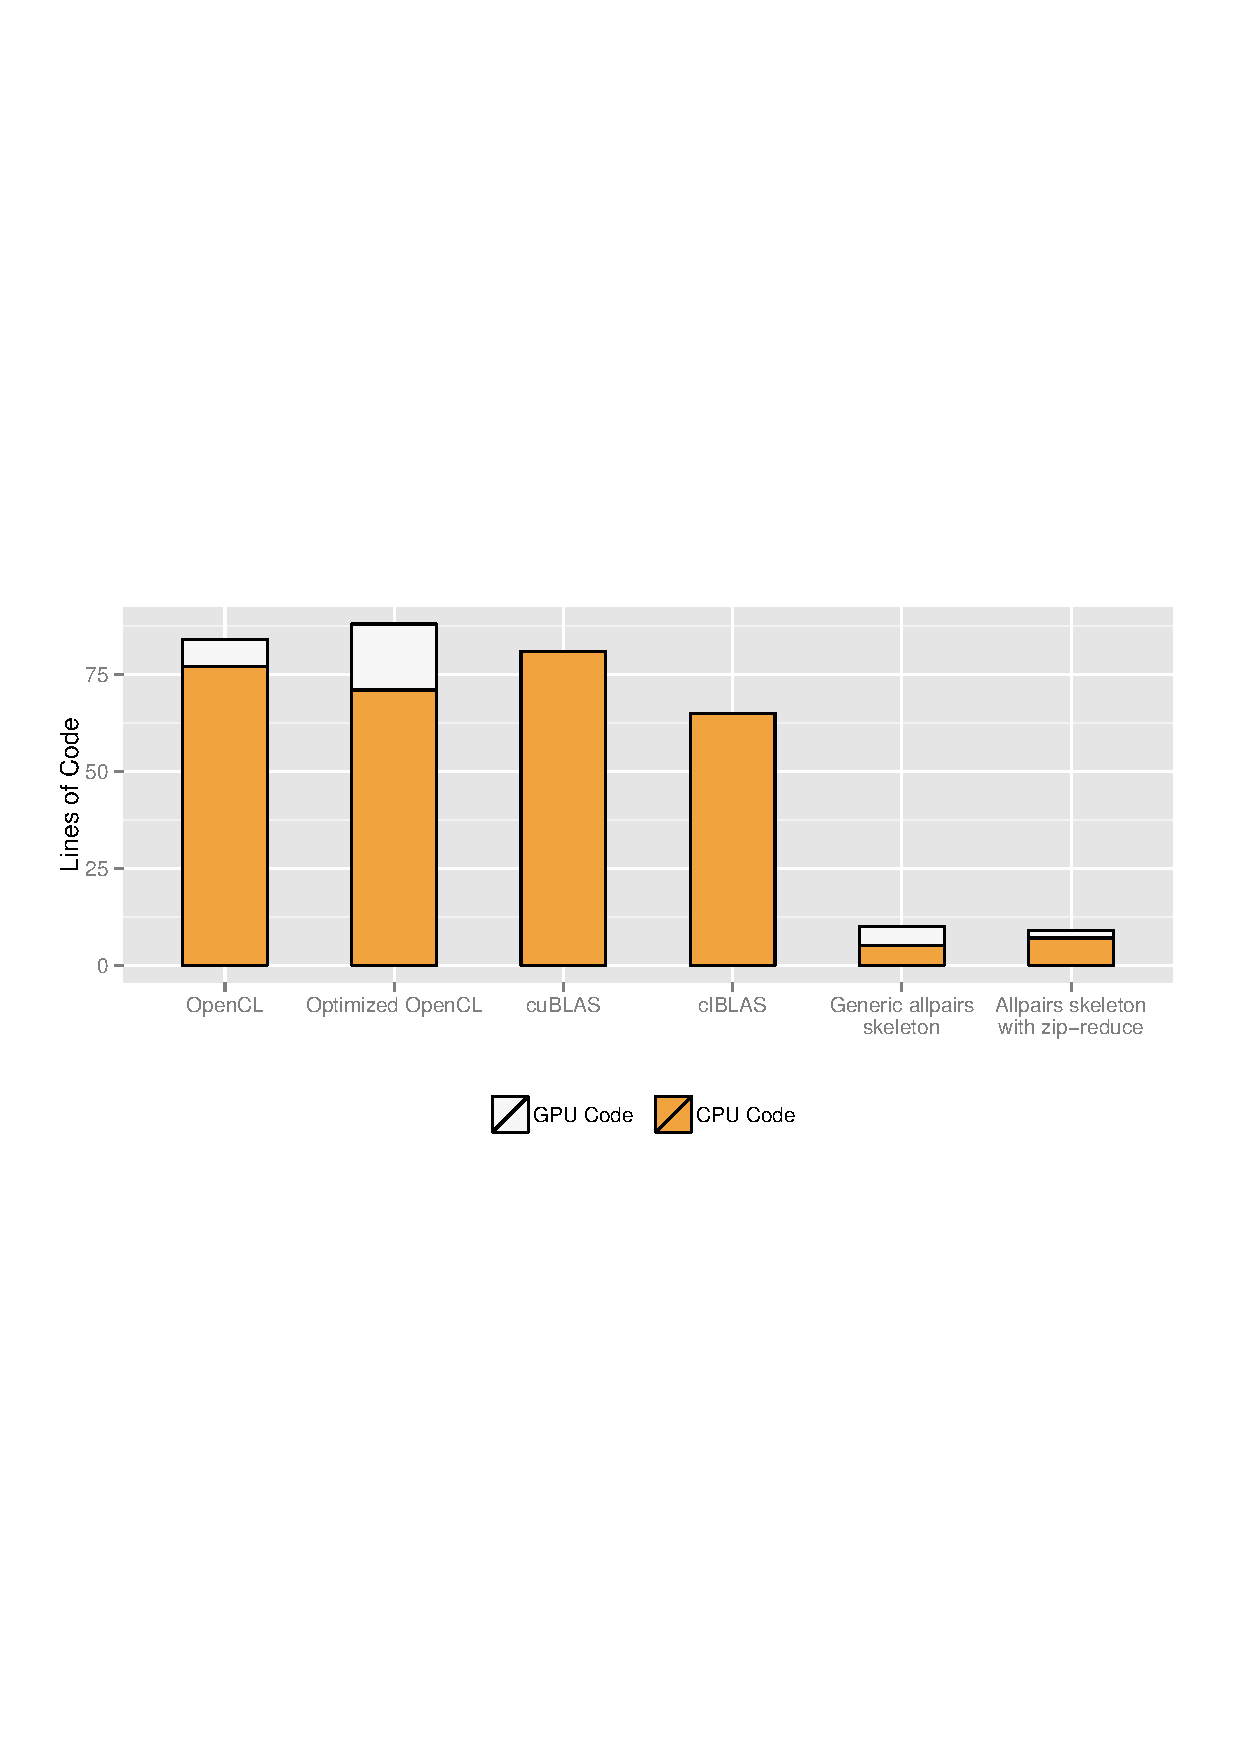
\includegraphics[width=\textwidth]{Plots/MatMult/mat_mult_loc}
  \caption[Programming effort of three \OpenCL-based, one \CUDA-base, and two \SkelCL-based matrix multiplication implementations.]%
          {Programming effort (Lines of Code) of three \OpenCL-based, and one \CUDA-based vs. two \SkelCL-based implementations.}
  \label{fig:mat_mult_loc}
  \end{minipage}
%\end{figure}
%\begin{table}[tb]
\strut\\[2em]\strut
  \begin{minipage}{\textwidth}
  \centering
  \begin{tabular}{lrrr}
    \toprule
              & \multicolumn{3}{c}{Lines of Code} \\
    \cmidrule(r){2-4}
    Implementation & \CPU & \GPU & Total \\[.5em]
    \midrule
    \OpenCL           & 77 &  7 & 84 \\[.5em]
    Optimized \OpenCL & 77 & 17 & 94 \\[.5em]
    \CUBLAS           & 81 & -- & 81\\[.5em]
    \clBLAS           & 65 & -- & 65\\[.5em]
    Generic \allpairs skeleton & 5 & 5 & 10\\[.5em]
    Specialized \allpairs skeleton & 7 & 2 & 9\\[.5em]
    \bottomrule
  \end{tabular}
  \captionof{table}%
          [Lines of Code for matrix multiplication implementaitons.]%
          {Lines of Code of all compared implementations.}
  \label{tab:mat_mult_loc}
  \end{minipage}
%\end{table}
\end{figure}

In the \OpenCL implementations, the \GPU code includes the kernel definition, as shown in \autoref{lst:naive_opencl} and \autoref{lst:local_mem_opencl};
the \CPU code includes the initialization of \OpenCL, memory allocations, explicit data transfer operations, and management of the execution of the kernel.

In the \BLAS implementations, the \CPU code contains the initialization of the corresponding \BLAS library, memory allocations, as well as a library call for performing the matrix multiplication;
no separate definition of \GPU code is necessary, as the \GPU code is defined inside the library function calls.

For the implementation based on the generic \allpairs skeleton (\autoref{lst:skelcl:mm:generic}), we count \autoref{lst:skelcl:mm:generic:CPU:start}---\autoref{lst:skelcl:mm:generic:CPU:stop} and \autoref{lst:skelcl:mm:generic:CPU:call} as the \CPU code, and the definition of the customizing function in \autoref{lst:skelcl:mm:generic:GPU:start}---\autoref{lst:skelcl:mm:generic:GPU:stop} as the \GPU code.
For the implementation based on the specialized \allpairs skeleton (\autoref{lst:skelcl:mm:special}), \autoref{lst:skelcl:mm:special:zipGPU} and \autoref{lst:skelcl:mm:special:reduceGPU} are the \GPU code, while all other lines constitute the \CPU code.

Both skeleton-based implementations are clearly the shortest, with 10 and 9 LOCs.
The next shortest implementation is the \CUBLAS implementation with 65 LOCs -- 7 times longer than the \SkelCL-based implementations.
The other implementations using \OpenCL require even 9 times more LOCs than the \SkelCL-based implementations.

Besides their length, the \OpenCL-based implementations require the application developer to explicitly implement many low-level, error-prone tasks, like dealing with pointers and offset calculations.
Furthermore, the skeleton-based implementations are more general, as they can be used for arbitrary allpairs computations, while all other implementations can compute matrix multiplication only.


\subsubsection*{Performance experiments}
We performed experiments with the six different implementations of matrix multiplication on two different computer systems with \GPUs:
\begin{itemize}[leftmargin=50pt]
  \item[System A:] Our general testing system already described in~\autoref{sec:skelcl:experimental_setup}:
    an Nvidia S1070 equipped with four Nvidia Tesla \GPUs, each with 240 streaming processors and 4 GByte memory.
  \item[System B:] An AMD Radeon HD 6990 card containing two \GPUs, each with 1536 streaming processors and 1 GByte memory.
\end{itemize}

\noindent
We include the data transfer times to and from the \GPU in the results. %, \ie the measured runtime consists of:
% 1) uploading the two input matrices to the \GPU;
% 2) performing the actual matrix multiplication;
% 3) downloading the computed result matrix.


\begin{figure}[tb]
  \centering
  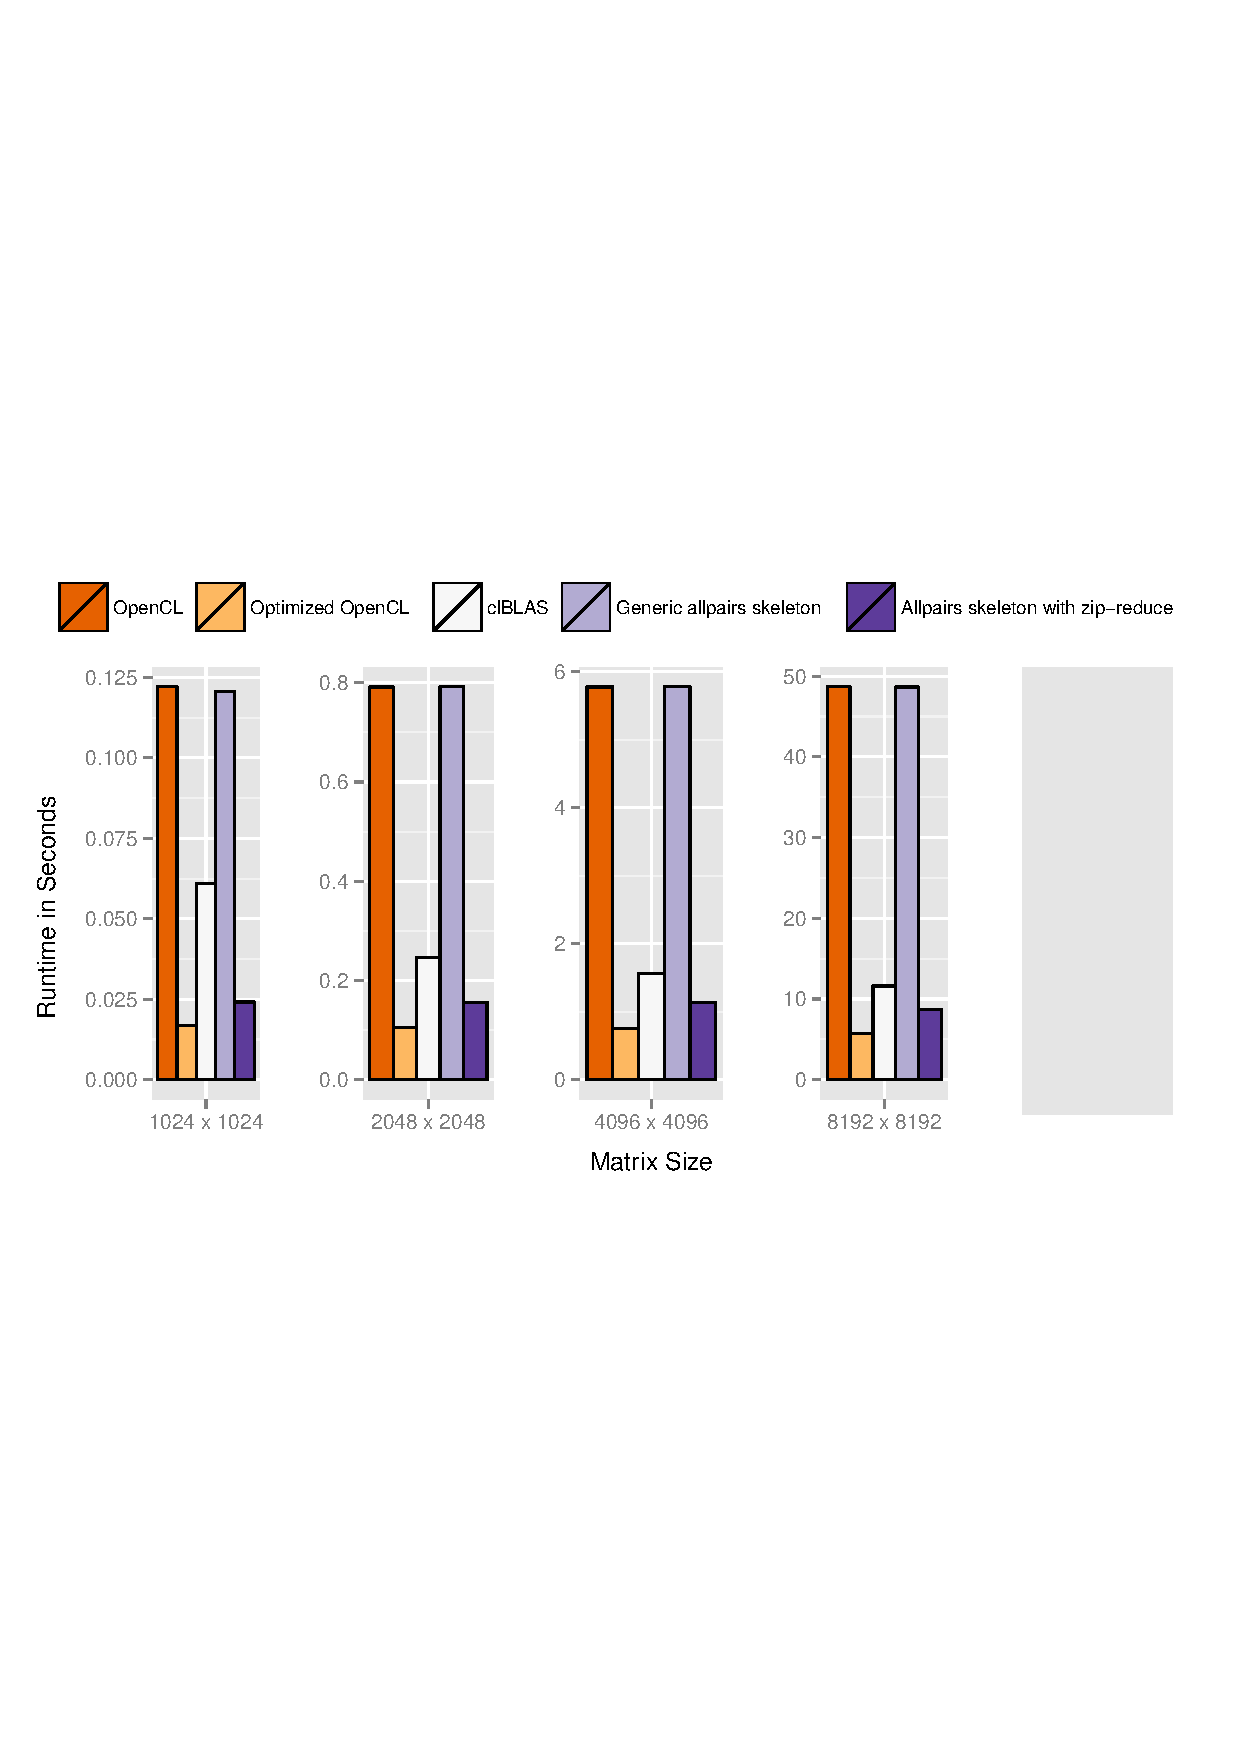
\includegraphics[width=0.8\textwidth]{Plots/MatMult/mat_mult_sizes_gtx480}
  \caption[Runtime of different matrix multiplication implementations on an Nvidia system.]%
          {Runtime of different matrix multiplication implementations on the Nvidia system for different sizes of the matrices.}
  \label{fig:mat_mult_single}
\end{figure}
\begin{table}[tb]
  \centering
  \begin{tabular}{lrrrrr}
    \toprule
              & \multicolumn{5}{c}{Runtimes in Seconds} \\
    \cmidrule(r){2-6}
    \multirow{2}{*}{Implementation} & $1024$ & $2048$ & $4096$ & $8192$ & $16384$ \\
                                    & $\times 1024$ & $\times 2048$ & $\times 4096$ & $\times 8192$ & $\times 16384$\\
    \midrule
    \OpenCL            & 0.122 & 0.791 & 5.778 & 48.682 & 472.557 \\
    Optimized \OpenCL  & 0.017 & 0.105 & 0.752 &  5.683 &  51.337 \\
    \CUBLAS            & 0.012 & 0.059 & 0.387 &  2.863 &  22.067 \\
    \clBLAS            & 0.061 & 0.246 & 1.564 & 11.615 &  90.705 \\
    Generic \allpairs  & \multirow{2}{*}{0.121} & \multirow{2}{*}{0.792} & \multirow{2}{*}{5.782} & \multirow{2}{*}{48.645} & \multirow{2}{*}{471.235} \\[-.5em]
    skeleton\\
    Specialized \allpairs & \multirow{2}{*}{0.024} & \multirow{2}{*}{0.156} & \multirow{2}{*}{1.134} & \multirow{2}{*}{8.742} & \multirow{2}{*}{68.544} \\[-.5em]
    skeleton\\
    \bottomrule
  \end{tabular}
  \caption[Runtime results for matrix multiplication on an Nvidia system.]
          {Runtime results for matrix multiplication on the Nvidia system.}
  \label{tab:mat_mult_single}
\end{table}

\paragraph{System A (one \GPU)}
\autoref{fig:mat_mult_single} shows the runtime of all six implementations for different sizes of the matrices (for readability reasons, all charts are scaled differently).
For detailed numbers, see \autoref{tab:mat_mult_single}.

Clearly, the naive \OpenCL implementation and the implementation using the generic \allpairs skeleton are the slowest, because both do not use local memory, in contrast to all other implementations.

The implementation using the specialized \allpairs skeleton performs 5.0 to 6.8 times faster than the generic allpairs skeleton, but is 33\% slower on the largest matrices than the optimized \OpenCL-based implementation. % using local memory.
However, the latter implementation can only be used for square matrices and, therefore, it benefits from omitting many conditional statements and boundary checks.


\CUBLAS is the fastest of all implementations, as it is highly tuned specifically for Nvidia \GPUs using \CUDA.
The \clBLAS implementation by AMD using \OpenCL performs not as well:
presumably, it is optimized for AMD \GPUs and performs poorly on other hardware.
Our optimized \allpairs skeleton implementation outperforms the \clBLAS implementation for all matrix sizes tested.


\pagebreak

\paragraph{System B (one \GPU)}
\autoref{fig:mat_mult_single_amd} shows the measured runtime in seconds for five of the six implementations for different sizes of the matrices.
Detailed numbers can be found in \autoref{tab:mat_mult_single_amd}.
We could not use the Nvidia-specific \CUBLAS implementation as it does not work on the AMD \GPU.

For bigger matrices, the slowest implementations are, again, the unoptimized \OpenCL implementation and the implementation using the generic \allpairs skeleton.

The optimized \OpenCL implementation and the specialized \allpairs skeleton perform similarly.
For matrices of size $8192\times 8192$, the optimized \OpenCL implementation is about 30\% faster.

The \clBLAS implementation performs very poorly for small matrices, but is clearly the fastest implementation for bigger matrices.
Similar to the \CUBLAS implementation on the Nvidia hardware, it is not surprising that the implementation by AMD performs very well on their own hardware.

\begin{figure}[tb]
  \centering
  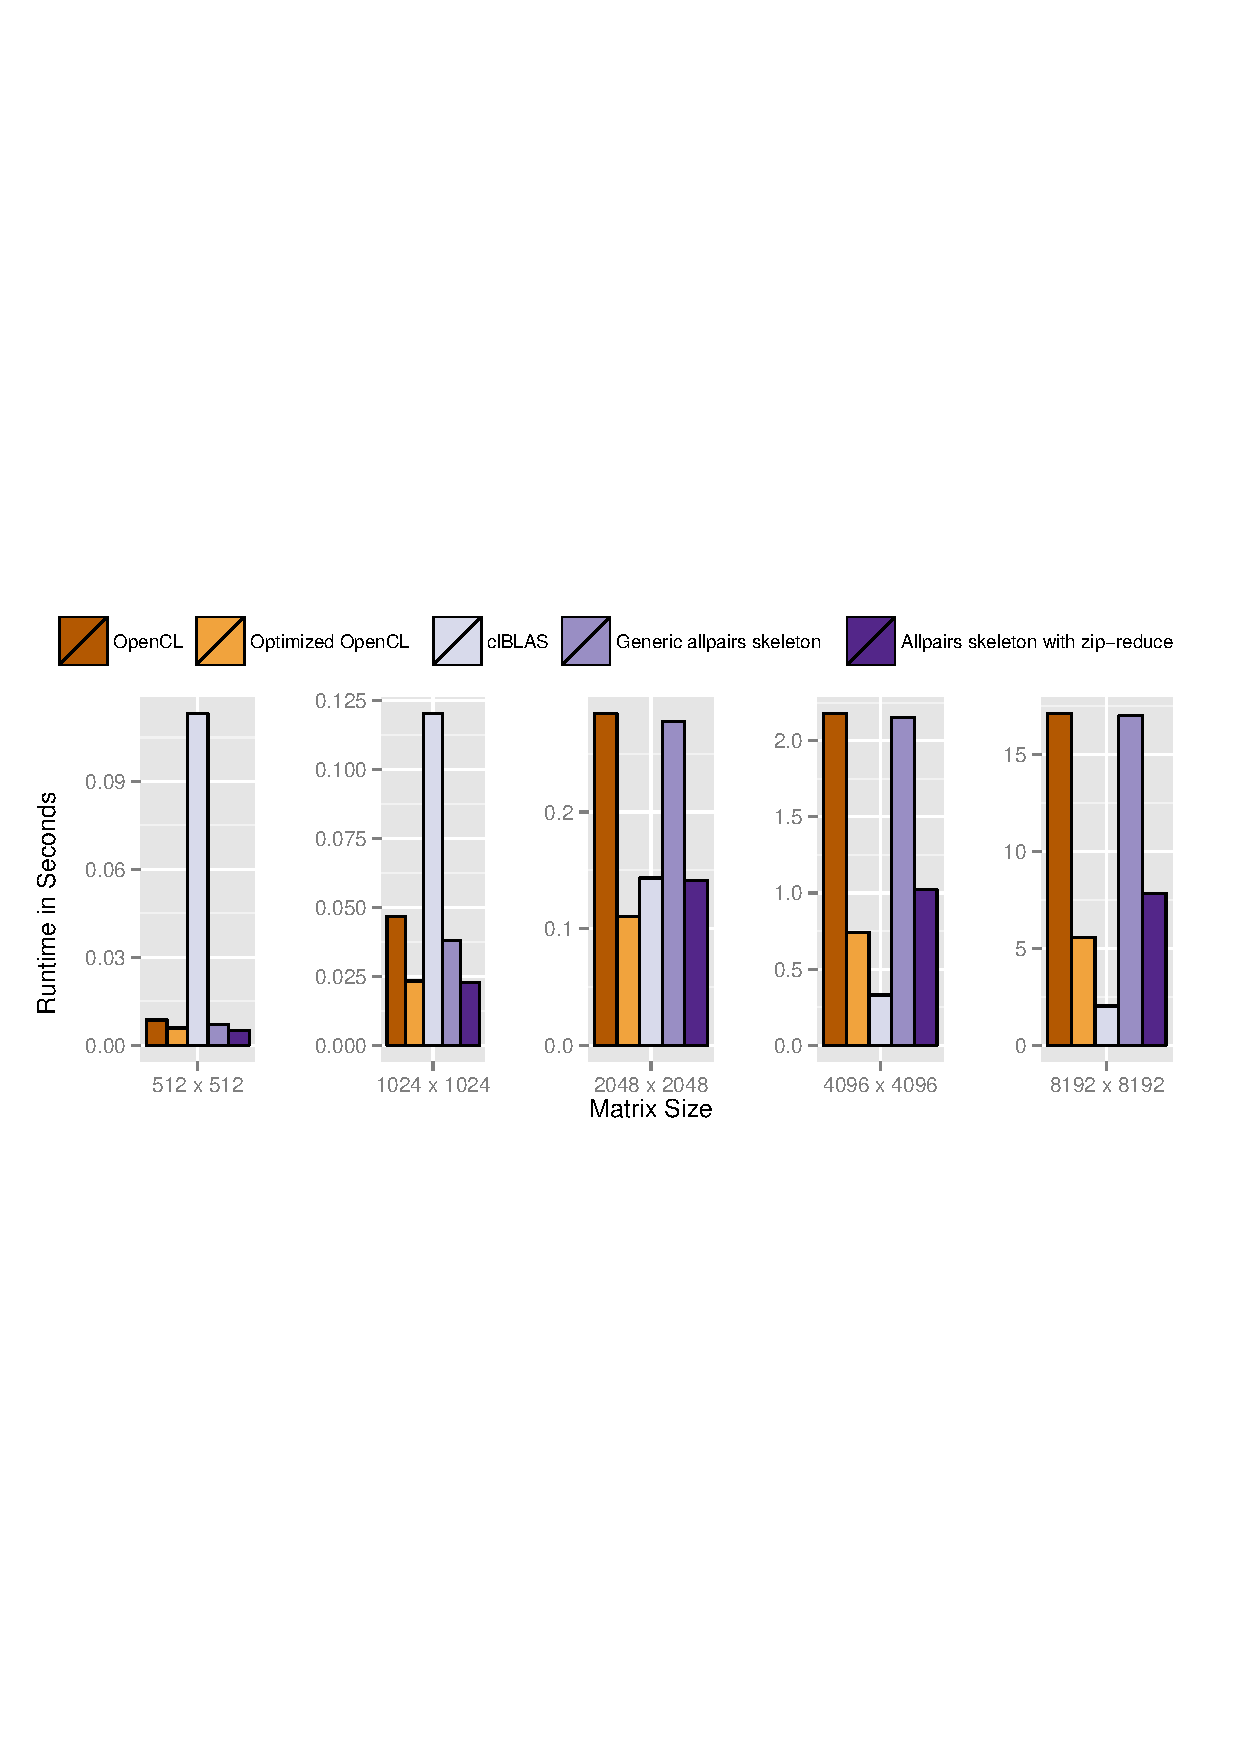
\includegraphics[width=0.8\textwidth]{Plots/MatMult/mat_mult_sizes_hd6990}
  \caption[Runtime of different matrix multiplication implementations on an AMD ststem.]%
          {Runtime of all compared implementations for a matrix multiplication on the AMD system using one \GPU.}
  \label{fig:mat_mult_single_amd}
\end{figure}
\begin{table}[tb]
  \centering
  \begin{tabular}{lrrrrr}
    \toprule
              & \multicolumn{5}{c}{Runtimes in Seconds} \\
    \cmidrule(r){2-6}
    \multirow{2}{*}{Implementation} & $512$ & $1024$ & $2048$ & $4096$ & $8192$ \\
                                    & $\times 512$ & $\times 1024$ & $\times 2048$ & $\times 4096$ & $\times 8192$ \\
    \midrule
    \OpenCL            & 0.008 & 0.046 & 0.284 & 2.178 & 17.098 \\
    Optimized \OpenCL  & 0.006 & 0.023 & 0.111 & 0.743 &  5.569 \\
    \clBLAS            & 0.113 & 0.120 & 0.143 & 0.329 &  2.029 \\
    Generic \allpairs  & \multirow{2}{*}{0.007} & \multirow{2}{*}{0.038} & \multirow{2}{*}{0.278} & \multirow{2}{*}{2.151} & \multirow{2}{*}{16.983} \\[-.5em]
    skeleton\\
    Specialized \allpairs & \multirow{2}{*}{0.005} & \multirow{2}{*}{0.023} & \multirow{2}{*}{0.141} & \multirow{2}{*}{1.025} & \multirow{2}{*}{7.842} \\[-.5em]
    skeleton\\
    \bottomrule
  \end{tabular}
  \caption[Runtime results for all tested implementations of matrix multiplication on an AMD system.]%
          {Runtime results for all tested implementations of matrix multiplication on the AMD system.}
  \label{tab:mat_mult_single_amd}
\end{table}


\pagebreak

\paragraph{System A (multiple \GPUs)}
\autoref{fig:mat_mult_devices} shows the runtime behavior for both \allpairs skeleton-based implementations when using up to four \GPUs of our multi-\GPU system.
The other four implementations are not able to handle multiple \GPUs and would have to be specially rewritten for such systems.
Newer versions of Nvidia's \CUBLAS implementation support the execution on multiple \GPUs as well.
We observe a good scalability for both of our skeleton-based implementations, achieving speedups between 3.09 and 3.93 when using four \GPUs.
Detailed numbers can be found in \autoref{tab:mat_mult_devices}.
For the matrices of size $16384\times 16384$, performance is also provided in GFlops;
to compute this value we excluded the data-transfer time (as usually done in related work) to enable better comparison with related work.

\begin{figure}[tb]
  \centering
  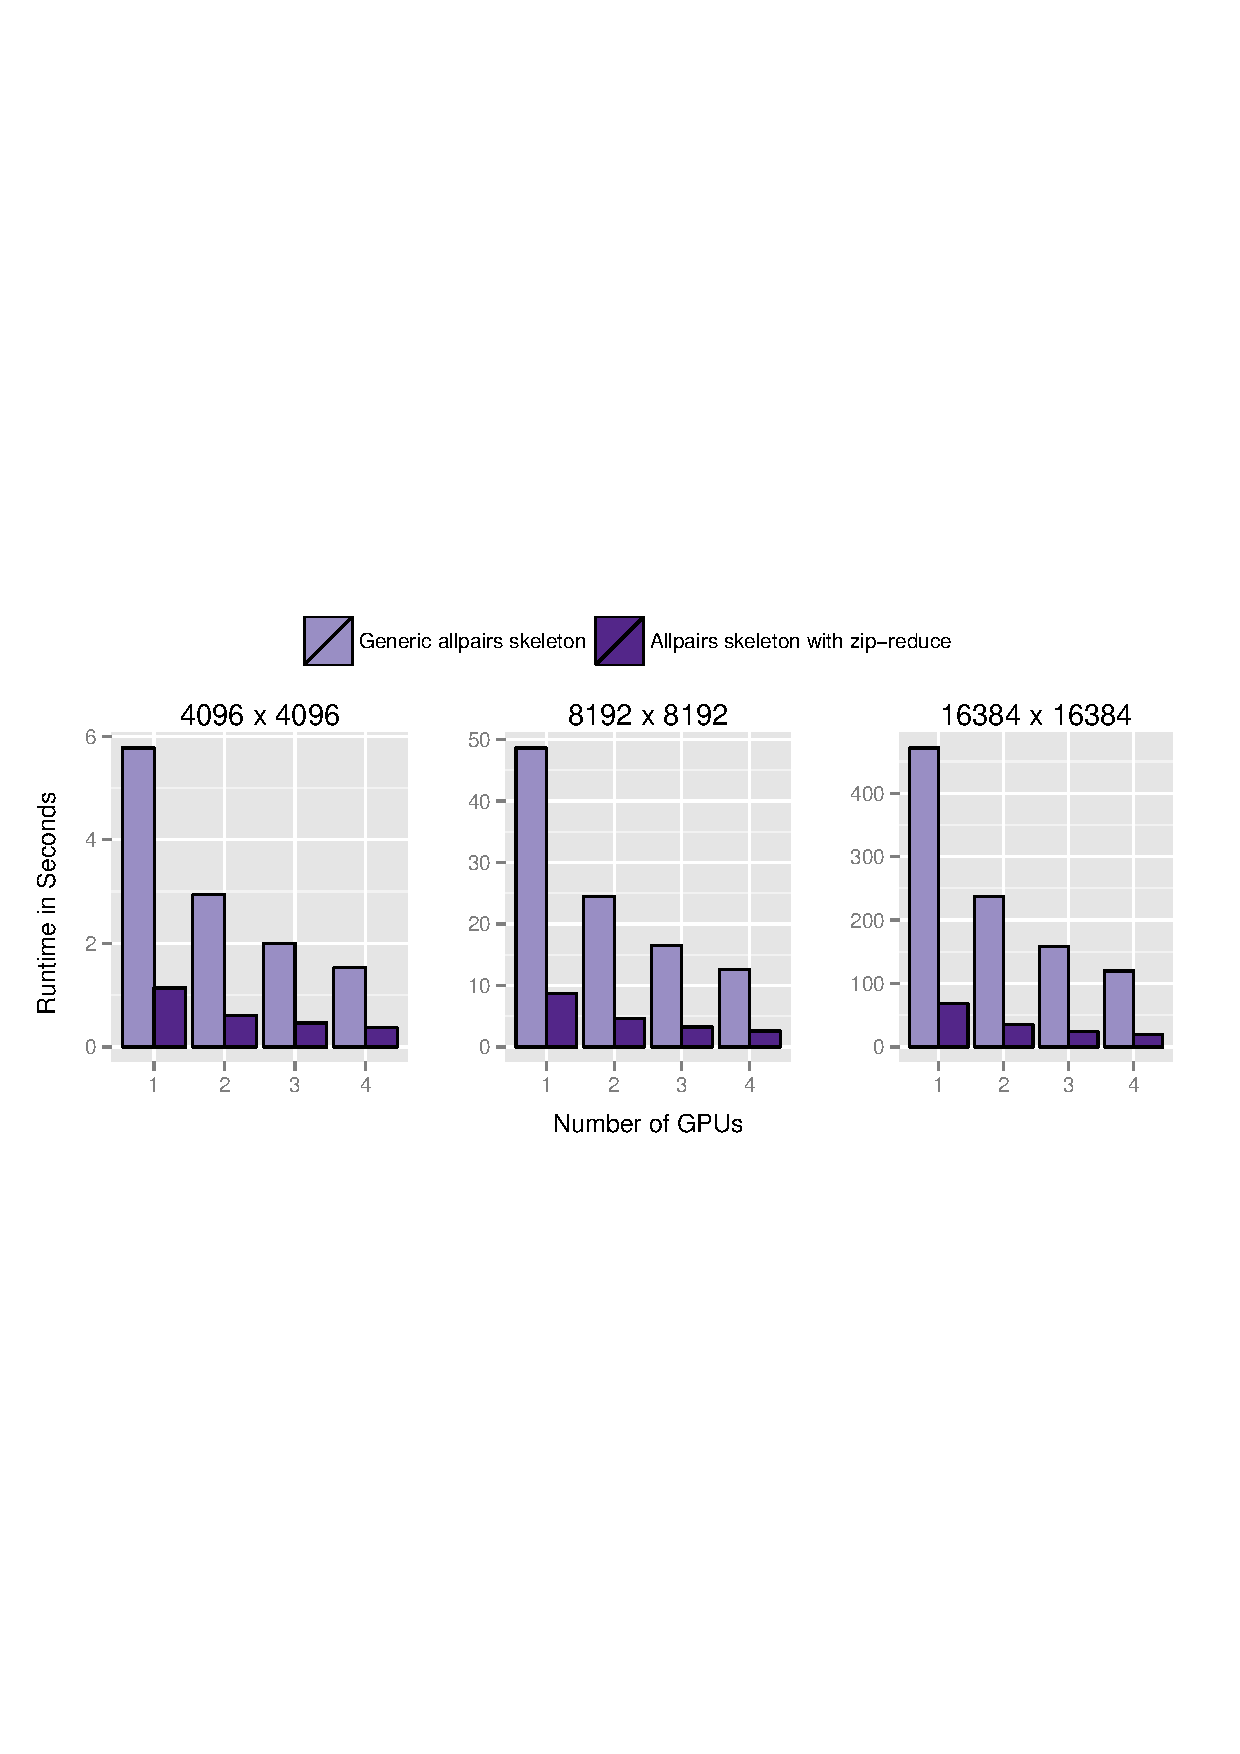
\includegraphics[width=0.9\textwidth]{Plots/MatMult/mat_mult_devices}
  \caption[Runtime of the \allpairs based matrix multiplication implementations using multiple \GPUs]%
          {Runtime of the \allpairs based implementations using multiple \GPUs.}
  \label{fig:mat_mult_devices}
\end{figure}
\begin{table}[tb]
  \centering
  \begin{tabular}{llrrrcr}
    \toprule
              & & \multicolumn{3}{c}{Runtimes in Seconds} & & GFlops\\
    \cmidrule(r){3-5}
    \cmidrule(r){7-7}
    \multirow{2}{*}{Implementation}
     & Number    & $4096$ & $8192$ & $16384$ & & $16384$\\
     & of \GPUs   & $\times 4096$ & $\times 8192$ & $ \times 16384$ & & $ \times 16384$\\
    \midrule
    \multirow{4}{*}{\parbox[t]{2.3cm}{Generic \allpairs\\ skeleton}}
     & 1 \GPU  & 5.772 & 48.645 & 471.328 &&  18.72\\
     & 2 \GPUs & 2.940 & 24.495 & 236.628 &&  37.43\\
     & 3 \GPUs & 2.000 & 16.532 & 158.611 &&  56.17\\
     & 4 \GPUs & 1.527 & 12.540 & 119.786 &&  74.90\\[.5em]
    \multirow{4}{*}{\parbox[t]{2.3cm}{Specialized \allpairs\\ skeleton}}
     & 1 \GPU  & 1.137 &  8.740 &  68.573 && 130.93\\
     & 2 \GPUs & 0.613 &  4.588 &  35.294 && 262.18\\
     & 3 \GPUs & 0.461 &  3.254 &  24.447 && 392.87\\
     & 4 \GPUs & 0.368 &  2.602 &  19.198 && 523.91\\
    \bottomrule
  \end{tabular}
  \caption[Runtime of the \allpairs based implementations of matrix multiplication using multiple \GPUs]%
   {Runtime of the \allpairs based implementations of matrix multiplication using multiple \GPUs.
    For the matrices of size $16384\times 16384$ the results are also shown in GFlops.}
  \label{tab:mat_mult_devices}
\end{table}

\FloatBarrier




\section{Image Processing Applications}
\label{sec:imageProcessing}
Many image processing applications are inherently parallel as they often independently process the pixels of an image.
Common examples range from simple thresholding over noise reduction applications to techniques used in edge detection and pattern recognition~\cite{Umbaugh1997}.
In this section we will study three application examples from image processing and how they can be implemented using \SkelCL.

We start by looking at the Gaussian blur application which can be used to reduce noise in images and is often used as a preprocessing step in more complex algorithms.
We will then discuss two algorithms used for edge detection in images:
the Sobel edge detection application and the more complex Canny edge detection algorithm.

These three applications can all be expressed using the \stencil skeleton introduced in \autoref{section:skelcl-programming-model:specialSkeletons}, but they have different characteristics.
The Gaussian blur applies a single stencil computation, possibly iterated multiple times, for reducing the noise in images.
The Sobel edge detection applies a stencil computation once to detect edges in images.
The more advanced Canny edge detection algorithm consists of a sequence of stencil operations which are applied to obtain the final result.
For each of the three applications, we compare the performance using our two implementations of the \stencil skeleton:
\code{MapOverlap} and \code{Stencil} with native OpenCL implementations using an input image of size $4096 \times 3072$.










\subsection{Gaussian Blur}
\label{sec:gauss}
The Gaussian blur is a standard algorithm used in image processing~\cite{Umbaugh1997}.
One common application is reduction of image noise as shown in \autoref{fig:lena:noise}.
%
\begin{figure}[tb]
  \centering
  \begin{subfigure}[t]{.45\textwidth}
    \includegraphics[width=\textwidth]{lenaNoise2}
    \caption{The Lena image with noise.}
    \label{fig:lena:noise:yes}
  \end{subfigure}
  \hfill
  \begin{subfigure}[t]{.45\textwidth}
    \includegraphics[width=\textwidth]{lenaNoNoise}
    \caption{The Lena image after applying the Gaussian blur.}
    \label{fig:lena:noise:no}
  \end{subfigure}
  \caption{Effect of applying the Gaussian blur to an noised image.}
  \label{fig:lena:noise}
\end{figure}
%
The image on the left has some noise as it is typically produced by halftone printing used to print newspapers.
The Gaussian blur has been applied to reduce the noise and produce the image on the right.

The Gaussian blur computes a weighted average for every pixel based on the neighboring pixels color values.
Using \SkelCL this application can easily be expressed using the \stencil skeleton.

\subsubsection*{\SkelCL Implementation}
\autoref{eq:gauss} shows the Gaussian blur expressed in the \SkelCL programming model using the \stencil skeleton.
\begin{align}
  gauss&\ M = stencil\ f\ 1\ \overline{0}\ M \qquad\text{where:}\nonumber\\
  &
  \begin{array}{ll}%
  f\ &\left[\begin{array}{lll}%
      \hspace{-.5em} M_{i-1,j-1}& \hspace{-.5em} M_{i-1,j} & \hspace{-.5em}M_{i-1,j+1}\vspace{-.25em}\\%
      \hspace{-.5em} M_{i,j-1}& \hspace{-.5em} M_{i,j} & \hspace{-.5em}M_{i,j+1}\vspace{-.25em}\\%
      \hspace{-.5em} M_{i+1,j-1}& \hspace{-.5em} M_{i+1,j} & \hspace{-.5em}M_{i+1,j+1}
    \end{array}\right]  = \\[2em]
          &\qquad \displaystyle\frac{\displaystyle\sum_{k=-1}^{1} \sum_{l=-1}^{1} (G\ k\ l)\cdot M_{i+k, j+k}}{9},
  \end{array} \label{eq:gauss}\\[1em]
  &G\ x\ y = \frac{1}{2\pi \sigma^{2}} e^{-\frac{x^2 + y^2}{2\sigma^2}} \nonumber\\
  \text{and } \overline{0} \text{ is th}&\text{e constant function always returning zero.}\nonumber
\end{align}
The function $G$ is the two-dimensional Gaussian function which is used in the customizing function $f$ to weight the neighboring values $M_{i,j}$.
The values obtained by applying $G$ can be precomputed, as $G$ is only evaluated with values in the interval $[-1, 1]$ for $x$ and $y$.


\autoref{lst:skelcl:gauss} shows the \SkelCL-based implementation of the Gaussian blur using the \code{MapOverlap} implementation of the \stencil skeleton.
Here the immediate neighboring pixels are accessed (lines~\ref{lst:skelcl:gauss:start}--\ref{lst:skelcl:gauss:end}) and used to compute a weighted value for each pixel.
The function computing the weighted sum is omitted here.
It is also possible to extend the \emph{range} of the Gaussian blur and include more neighboring pixel values in the computation.

\begin{lstlisting}[%                                                             
caption={Implementation of the Gaussian blur in \SkelCL using the \code{MapOverlap} implementation of the \stencil skeleton.},%
numbers=left,%
float=tb,
label={lst:skelcl:gauss}]
Matrix<char> gaussianBlur(const Matrix<char>& image) {
  auto gauss = mapOverlap(
    [](Neighborhood<char>& in) {
      char ul = in[{-1, -1}];$\label{lst:skelcl:gauss:start}$
      ...
      char lr = in[{+1, +1}];$\label{lst:skelcl:gauss:end}$
      return computeGaussianBlur(ul, ..., lr); },
    1, BorderHandling::NEUTRAL(0));
  return gauss(image); }
\end{lstlisting}

\subsubsection*{Programming effort}

\begin{figure}[tbp]
	\centering
	\includegraphics[width=\columnwidth]{Plots/gauss/gauss_loc.pdf}
	\caption[Lines of code of the Gaussian blur using different implementations.]%
          {Lines of code of the Gaussian blur using a na{\"i}ve OpenCL implementation with global memory, an optimized OpenCL version using local memory, and \SkelCL's \code{MapOverlap} and \code{Stencil} implementations of the \stencil skeleton.}
	\label{fig:gaussLOCs}
\end{figure} 

\autoref{fig:gaussLOCs} shows the program sizes (in lines of code) for the four implementations of the Gaussian blur. 
The application developer needs $57$ lines of OpenCL host code and 13 LOCs for performing a Gaussian blur only using global memory. 
When using local memory, some more arguments are passed to the kernel, thus, increasing the host-LOCs to $65$, while the LOCs for the kernel function, which copies all necessary elements for a work-group's calculation into local memory, requires $88$ LOCs including explicit out-of-bounds handling and complex index calculations.
The \code{MapOverlap} and \code{Stencil} versions are similar and both require only $15$ LOCs host code and $9$ LOCs kernel code to perform a Gaussian blur. 
The support for multi-\GPU systems is implicitly provided when using \SkelCL's skeletons, such that the kernel remains the same as for one-\GPU systems.
This is an important advantage of \SkelCL over the \OpenCL implementations of the Gaussian blur which are single-\GPU only and require additional LOCs when adapting them for multi-\GPU environments.

\subsubsection*{Performance experiments}

\begin{figure}[tbp]
	\centering
	\includegraphics[width=\columnwidth]{Plots/gauss/gauss_runtime.pdf}
	\caption[Runtime of the Gaussian blur using different implementations.]%
          {Runtime of the Gaussian blur using a na{\"i}ve OpenCL implementation with global memory, an OpenCL version using local memory and SkelCL's MapOverlap and Stencil skeletons.}
	\label{fig:gaussAbs}
\end{figure} 

\autoref{fig:gaussAbs} shows the measured total runtime including data transfers of the Gaussian blur using:
\begin{itemize}
  \item[1)] a na{\"i}ve OpenCL implementation using global memory,
  \item[2)] an optimized OpenCL version using local memory,
  \item[3)] \code{MapOverlap}-based implementation, and
  \item[4)] the \code{Stencil}-based implementation, correspondingly.
\end{itemize}
We can observe that for larger stencil shape sizes, the \code{MapOverlap} and \code{Stencil}-based versions outperform the na{\"i}ve OpenCL implementation by $65\%$ and $62\%$, respectively.
The optimized OpenCL version, which copies all necessary elements into local memory prior to calculation, is $5\%$ faster than \code{MapOverlap} and $10\%$ faster than \code{Stencil} for small stencil shapes.
When increasing the stencil shape size, this disadvantage is reduced to $3\%$ for \code{MapOverlap} and $5\%$ for \code{Stencil} with stencil shape's extent of $10$ in each direction.

The \code{Stencil} implementation is slower for small stencil shapes than the \code{MapOverlap} implementation, up to $32\%$ slower for an stencil shape size of $1$.
This is due to the increased branching required in the \code{Stencil} implementation, as discussed in more detail in \autoref{sec:skelcl:stencil}.
However, this disadvantage is reduced to $4.2\%$ for the stencil shape size of $5$ and becomes negligible for bigger stencil shape sizes.
% Due to the increased branching in Stencil's kernel function, one might expect a worse runtime for the Stencil skeleton. 
As the ratio of copying into local memory decreases in comparison to the number of calculations when enlarging the stencil shape's size, the kernel function's runtime in the \code{Stencil} implementation  converges to the \code{MapOverlap} implementation's time.
The \code{Stencil} implementation's disadvantage is also due to its ability to manage multiple stencil shapes and explicitly support the use of iterations.
While both features are not used in this application example, they incur some overhead for the implementation as compared to the \code{MapOverlap} implementation for simple stencil computations.


\autoref{fig:GaussMult} shows the speedup achieved on the Gaussian blur using the \code{Stencil} implementation on up to four devices.
The higher the computational complexity for increasing size of stencil shape, the better the overhead is hidden, leading to a maximum speedup of $1.90$ for two devices, $2.66$ for three devices, and $3.34$ for four devices, for a size of the stencil shape of 20.
\begin{figure}
	\centering
	\includegraphics[width=.85\columnwidth]{Plots/gauss/gauss_speedup.pdf}
	\caption{Speedup of the Gaussian blur application on up to four \GPUs.}
	\label{fig:GaussMult}
\end{figure} 










\subsection{Sobel Edge Detection}
\label{sec:sobel}
The Sobel edge detection produces an output image in which the detected edges in the input image are marked in white and plain areas are shown in black.
The effect is shown in \autoref{fig:sobel:lena}, where the original image is shown on the left and the output of Sobel edge detection applied to it on the right.

\begin{figure}[tb]
  \centering
  \begin{subfigure}[t]{.45\textwidth}
    \includegraphics[width=\textwidth]{Paraphrase/lena.png}
    \caption{Original image.}
    \label{fig:lena:orig}
  \end{subfigure}
  \hfill
  \begin{subfigure}[t]{.45\textwidth}
    \includegraphics[width=\textwidth]{Paraphrase/sobel_filtered-lena.png}
    \caption{Image after Sobel edge detection.}
    \label{fig:lena:sobel}
  \end{subfigure}
  \caption[The Lena image before and after applying Sobel edge detection.]%
          {The Lena image~\cite{Lena} often used as an example in image processing before (left) and after (right) applying Sobel edge detection.}
  \label{fig:sobel:lena}
\end{figure}

\begin{lstlisting}[%
caption={Sequential implementation of the Sobel edge detection.},%
float=tb,
label={lst:sobel:seq}]
for (i = 0; i < width; ++i)
  for (j = 0; j < height; ++j)
    h = -1*img[i-1][j-1] +1*img[i+1][j-1]
        -2*img[i-1][j  ] +2*img[i+1][j  ]
        -1*img[i-1][j+1] +1*img[i+1][j+1];
    v = ...;
    out_img[i][j] = sqrt(h*h + v*v);
\end{lstlisting}
\bigskip

\autoref{lst:sobel:seq} shows the sequential algorithm of the Sobel edge detection in pseudo-code, with omitted boundary checks for clarity.
In this version, for computing an output value \code{out\_img[i][j]} the input value \code{img[i][j]} and the direct neighboring elements are weighted and summed up horizontally and vertically.
The \stencil skeleton is a perfect fit for implementing the Sobel edge detection.

\subsubsection*{\SkelCL Implementation}
\autoref{eq:sobel} shows the implementation of the Sobel edge detection in the \SkelCL programming model.
\begin{align}
  \label{eq:sobel}
  sobel\ M& = stencil\ f\ 1\ \overline{0}\ M \qquad\text{where:}\\
  f\ &\left[\begin{array}{lll}%
      \hspace{-.5em} M_{i-1,j-1}& \hspace{-.5em} M_{i-1,j} & \hspace{-.5em}M_{i-1,j+1}\vspace{-.25em}\\%
      \hspace{-.5em} M_{i,j-1}& \hspace{-.5em} M_{i,j} & \hspace{-.5em}M_{i,j+1}\vspace{-.25em}\\%
      \hspace{-.5em} M_{i+1,j-1}& \hspace{-.5em} M_{i+1,j} & \hspace{-.5em}M_{i+1,j+1}
    \end{array}\right] = \displaystyle\sqrt{ h^2 + v^2 }\nonumber\\
  h & = \sum_{k=0}^2 \sum_{l=0}^2 Gx_{k, l}\cdot M_{i+k-1,j+k-1}\nonumber\\
  v & = \sum_{k=0}^2 \sum_{l=0}^2 Gy_{k, l}\cdot M_{i+k-1,j+k-1}\nonumber\\
  Gx& = \left[\begin{array}{ccc}%
      -1&0&+1\\
      -2&0&+2\\
      -1&0&+1
    \end{array}\right]
  Gy = \left[\begin{array}{ccc}%
      -1&-2&-1\\
      0&0&0\\
      +1&+2&+1
    \end{array}\right] \nonumber\\
  \text{and } \overline{0} \text{ is th}&\text{e constant function always returning 0.}\nonumber
\end{align}
The formula resembles the sequential implementation shown in \autoref{lst:sobel:seq} where the final result is computed as the square root of the sum of two squared terms $h$ and $v$.
These are computed as weighted sums of the neighboring values $M_{i,j}$.
The weights are given by the two matrices $Gx$ and $Gy$.

\autoref{lst:sobel:skelcl} shows the \SkelCL implementation using the \code{MapOverlap} implementation of the \stencil skeleton.
%
\begin{lstlisting}[%
caption={\SkelCL implementation of the Sobel edge detection.},%
numbers=left,
float=tb,
label={lst:sobel:skelcl}]
Matrix<char> sobelEdge(const Matrix<char>& image) {
  auto sobel = mapOverlap(
    [](Neighborhood<char>& in) {
      short h = -1*in[{-1,-1}] +1*in[{+1,-1}]
                -2*in[{-1, 0}] +2*in[{+1, 0}]
                -1*in[{-1,+1}] +1*in[{+1,+1}];
      short v = ...;
      return sqrt(h*h + v*v); },
    1, BorderHandling::NEUTRAL(0));
  return soble(img); }
\end{lstlisting}
%
The implementation is straightforward and very similar to the formula in \autoref{eq:sobel} and the sequential version in \autoref{lst:sobel:seq}.

\subsubsection*{Programming effort}

\begin{lstlisting}[%
caption={Additional boundary checks and index calculations for Sobel algorithm, necessary in the standard OpenCL implementation.},%
float=tb,
numbers=left,
label={lst:sobel:opencl}]
kernel void sobel_kernel( global const uchar* img,
                          global       uchar* out_img) {
 uint i = get_global_id(0);   uint j = get_global_id(1);
 uint w = get_global_size(0); uint h = get_global_size(1);
 // perform boundary checks
 if(i >= 1 && i < (w-1) && j >= 1 && j < (h-1)) {
  char ul = img[((j-1)*w)+(i-1)];
  char um = img[((j-1)*w)+(i+0)];
  char ur = img[((j-1)*w)+(i+1)];
  // ... 5 more
  char lr = img[((j+1)*w)+(i+1)];

  out_img[j * w + i] = computeSobel(ul, um, ur, ..., lr); }}
\end{lstlisting}

\autoref{lst:sobel:opencl} shows a part of the rather simple \OpenCL implementation for Sobel edge detection provided by AMD as an example application in their software development kit~\cite{AMDSDK}.
The actual computation is performed inside the \texttt{computeSobel} function, which is omitted in the listing, since it is quite similar to the sequential version in \autoref{lst:sobel:seq}.
The listing shows that extra low-level code is necessary to deal with technical details, like boundary checks and index calculations, which are arguably quite complex and error-prone.

We also compare against a more optimized \OpenCL implementation by Nvidia which makes use of the fast local \GPU memory.

The \SkelCL implementation is significantly shorter than the two \OpenCL-based implementations.
The \SkelCL program only comprises few lines of code as shown in \autoref{lst:sobel:skelcl}.
The AMD implementation requires 37 lines of code for its kernel implementation and the more optimized Nvidia implementation requires even 208 lines of code.
Both versions require additional lines of code for the host program which manages the execution of the \OpenCL kernel.
No index calculations or boundary checks are necessary in the \SkelCL version whereas they are crucial for a correct implementation in \OpenCL.

\subsubsection*{Performance experiments}

\begin{figure}[tbp]
  \vspace{.5em}
  \centering
  \includegraphics[height=4.5cm]{Plots/Sobel/sobel_runtime.pdf}
  \caption{Performance results for Sobel edge detection}
  \label{fig:sobel:measurements}
\end{figure}
\autoref{fig:sobel:measurements} shows the measured runtime of the two \OpenCL versions (from the AMD and Nvidia SDKs) vs. the \SkelCL version with the \stencil skeleton presented in \autoref{lst:sobel:skelcl}.
Here only the kernel runtimes are shown, as the data transfer times are equal for all versions.
We used the popular Lena image~\cite{Lena} with a size of $512\times 512$ pixel as an input.
The AMD version is clearly slower than the two other implementations, because it does not use the fast local memory which the Nvidia implementation and the \code{MapOverlap} implementation of the \stencil skeleton of \SkelCL do.
\SkelCL completely hides the memory management details inside its implementation from the application developer.
The Nvidia and \SkelCL implementations perform similarly fast.
In this particular example, \SkelCL even slightly outperforms the implementation by Nvidia.










\subsection{Canny Edge Detection}
The Canny edge detection algorithm is a more complex algorithm to detect edges in images than the Sobel edge detection presented in the previous section.
For the sake of simplicity we consider a slightly simplified version, which applies the following stencil operations in a sequence:
1), a noise reduction operation is applied, \eg, a Gaussian blur;
2), an edge detection operator like the Sobel edge detection is applied;
3), the so-called non-maximum suppression is performed, where all pixels in the image are colored black except pixels being a local maximum;
4), a threshold operation is applied to produce the final result.
A more complex version of the algorithm performs the edge tracking by hysteresis, as an additional step.
This results in detecting some weaker edges, but even without this additional step the algorithm usually achieves good results.


\subsubsection*{\SkelCL Implementation}
In \SkelCL, each single step of the Canny algorithm can be expressed using the \stencil skeleton.
The last step, the threshold operation, does not need access to neighboring elements, as the user threshold function only checks the value of the current pixel.
Therefore, this step can be expressed using \SkelCL's simpler \map skeleton.
In the \SkelCL library the \code{Stencil} skeleton's implementation automatically uses the simpler \map skeleton's implementation when the user specifies a stencil shape which extents are $0$ in all directions.

\begin{lstlisting}[%
  caption={Structure of the Canny algorithm expressed as a sequence of skeletons.},%
  float=tbp,%
  label={lst:skelcl:canny}]
Matrix<char> sobelEdge(const Matrix<char>& image) {
  auto gauss     = stencil(...);$\label{lst:skelcl:canny:step1}$
  auto sobel     = stencil(...);
  auto nms       = stencil(...);
  auto threshold = stencil(...);$\label{lst:skelcl:canny:stepN}$
  StencilSequence<Pixel(Pixel)>
      canny(gauss, sobel, nms, threshold);$\label{lst:skelcl:canny:combine}$
  return canny(image); }$\label{lst:skelcl:canny:call}$
\end{lstlisting}

To implement the Canny algorithm in \SkelCL, the single steps can be combined as shown in \autoref{lst:skelcl:canny}.
The individual steps are defined in lines~\ref{lst:skelcl:canny:step1}--\ref{lst:skelcl:canny:stepN} and then combined to a sequence of stencils in line~\ref{lst:skelcl:canny:combine}.
During execution (line~\ref{lst:skelcl:canny:call}), the stencil operations are performed in the order which is specified when creating the \code{StencilSequence} object.

%\subsubsection*{Programming effort}

\subsubsection*{Performance experiments}

\begin{figure}[tbp]
	\centering
	\includegraphics[width=.75\columnwidth]{Plots/Canny/canny_runtime.pdf}
	\caption[Runtime of the Canny edge detection algorithm.]%
          {Runtime of the Canny edge detection algorithm comparing the \code{MapOverlap} and \code{Stencil} skeleton implementations.}
	\label{fig:canny}
\end{figure} 

\autoref{fig:canny} shows the measured runtime of the Canny algorithm using the two presented implementations.
As the \code{MapOverlap} implementation appends padding elements to the matrix representing the image, the matrix has to be downloaded, resized and uploaded again to the \GPU between every two steps of the sequence.
This additional work leads to an increased time for data transfers. 
The Gaussian blur with a stencil shape extent of $2$, as well as the Sobel edge detection and the non-maximum suppression with a stencil shape of $1$, are $2.1$ to $2.2$ times faster when using \code{MapOverlap}. 
However, the threshold operation, which is expressed as the \map skeleton in the Stencil sequence, is $6.8$ times faster than \code{MapOverlap}'s threshold operation.
Overall, we observe that when performing sequences of stencil operations, the \code{Stencil} implementation reduces the number of copy operations and, therefore, leads to a better overall performance.
When performing the Canny algorithm, the \code{Stencil} implementation outperforms the \code{MapOverlap} implementation by $21\%$.



\section{Medical Imaging}

\from{HIPS begin}
\subsection{List-mode OSEM (HIPS)}

\emph{List-Mode Ordered Subset Expectation Maximization} (list-mode OSEM) is a time-intensive, production-quality algorithm from a real-world application in medical image reconstruction.
It is used to reconstruct three-dimensional images from huge sets of so-called \emph{events} recorded in \emph{positron emission tomography} (PET).
Each event represents a \emph{line of response} (LOR) which intersects the scanned volume.
A simplified sequential implementation of list-mode OSEM is shown in Listing~\ref{lst:lmosem_seq}.
The algorithm splits the events into \emph{subsets} which are processed iteratively:
All LORs of a subset's events and their corresponding intersection \emph{paths} are computed and merged into an \emph{error image} which is merged with the reconstruction image, thus refining a \emph{reconstruction image} in each iteration.

\begin{lstlisting}[%
caption={Sequential implementation of list-mode OSEM.},%
float=bp,%
label={lst:lmosem_seq}]
for	(l = 0; l < num_subsets; l++) {
	/* read subset from file */
	events = read_events();
	/* compute error image c */
	for	(i = 0; i < num_events; i++) {
		/* compute path of LOR */
		path = compute_path(events[i]);
		/* compute error */
		for	(fp = 0, m = 0; m<path_len; m++)
			fp += f[path[m].coord] * path[m].len;
		/* add path to error image */
		for (m = 0; m<path_len; m++)
			c[path[m].coord] += path[m].len / fp;
	}
	/* update reconstruction image f */
	for	(j = 0; j < image_size; j++)
		if (c[j] > 0.0) f[j] *= c[j];	}
\end{lstlisting}

In a parallel implementation of list-mode OSEM, the loops for calculating the error image ($c$) and for updating the reconstruction image ($f$) can be parallelized.

\subsubsection{Programming effort}

We develop implementations of list-mode OSEM using OpenCL and SkelCL; a CUDA-based implementation using multiple GPUs has already been implemented~\cite{ScVG-08}.
Both, CUDA and OpenCL, require us to add a considerable amount of boilerplate code for running a kernel on multiple GPUs, in particular for uploading and downloading data to and from the GPUs.
In CUDA, we have to create one CPU thread for each device to be managed.
This introduces the additional challenge of multi-threaded programming, including the need of thread synchronization.

\begin{lstlisting}[%
caption={Implementation of list-mode OSEM in SkelCL.},%
float=tbp,%
label={lst:lmosem_skelcl}]
for (l = 0; l < num_subsets; l++) {
	// read events from file
	Vector<Event> events(read_events());
	
	// distribute events to devices
	events.setDistribution(
		Distribution::block);
	// copy reconstruction (f) and error image (c) to all devices
	f.setDistribution(Distribution::copy);
	c.setDistribution(Distribution::copy);
	
	// prepare arguments of error image computation
	SkelCL::Arguments arguments;
	arguments.push(events);
	arguments.push(events.size());
	arguments.push(paths); // memory for paths
	arguments.push(f);
	arguments.push(c);
	
	// compute error image (map skeleton)
	compute_c(index, arguments);
	
	// signal modification of error image
	c.dataOnDevicesModified();
	// distribute reconstruction image to  all devices
	f.setDistribution(Distribution::block);
	// reduce (element-wise add) all copies of error image; re-distribute to all devices after reduction
	c.setDistribution(Distribution::block, add);
	
	// update reconstruction image (zip skeleton)
	update(f, c, f);	}
\end{lstlisting}

With SkelCL, we use the \texttt{Vector} class and the \texttt{Map} and \texttt{Zip} skeletons to implement list-mode OSEM (see Listing~\ref{lst:lmosem_skelcl}).
The events of a subset, as well as the error image and the reconstruction image are stored in a SkelCL \texttt{Vector}.
Thus, we can easily distribute subsets across all GPUs and copy both images to all devices.
We use a \texttt{Map} skeleton to implement the computation of the error image.
However, we must not compute too many paths in parallel to avoid excessive memory consumption.
Therefore, the input of the \texttt{Map} skeleton is not a subset, but rather a vector of 512 indices.
These indices refer to disjoint sub-subsets of events, each of which is processed within a single kernel instance on the GPUs.
For each event, this kernel performs the same steps as the first inner loop in the sequential implementation.
The reconstruction and the error image, as well as the events, are passed to the \texttt{Map} skeleton as additional arguments.
The skeleton produces no result, but updates the error image by side-effect.
Therefore, the error image has to be marked as ``modified on the device'' after executing the \texttt{Map} skeleton.

So far, separate copies of the error image have been used on all GPUs.
To obtain the final error image, we have to merge all copies into a single image.
Afterwards, the final error image and the reconstruction image are distributed across all GPUs, such that each device processes a part of these images.
In SkelCL, the aforementioned data movement is easily achieved by changing the kind of distribution of the vectors that contain this data.
A \texttt{Zip} skeleton is used to implement the update of the reconstruction image, taking the distributed images as input.
The kernel function of this skeleton resembles the body of the second inner loop of the sequential implementation.

The parallelization using SkelCL is quite similar to our CUDA- and OpenCL-based implementations.
However, when using SkelCL's vector data type, we avoid additional programming effort to implement data transfer between host and GPU or between multiple GPUs, and we obtain a multi-GPU-ready implementation of list-mode OSEM for free.
The SkelCL-based implementation is the shortest with 232 lines of code (kernel function: 200~lines, host program: 32~lines).
The CUDA- and OpenCL-based implementations are considerably longer with 329 (199, 130), or even 436 lines of code (193, 243), respectively (see Figure~\ref{fig:lmosem_results}).


\subsubsection{Performance experiments}

We tested our implementations of list-mode OSEM using a typical data set of about $10^7$ events for $150\times 150\times 280$ PET image.
The data set is split into 10 equally sized subsets.
We measured the average runtime of processing all subsets.
Figure~\ref{fig:lmosem_results} shows the runtime of our three implementations of list-mode OSEM using one, two, and four GPUs.

\begin{figure}[tbp]
	\centering
	\label{fig:lmosem_runtime}%
	\label{fig:lmosem_speedup}%
	\includegraphics[width=0.42\textwidth]{HIPS/ChartLmosem}
	\caption{Runtime and program size of parallel list-mode OSEM using CUDA, OpenCL, and SkelCL.}
	\label{fig:lmosem_results}
\end{figure}

Running on a single GPU, the CUDA-based implementation (3.03 seconds) outperforms the ones based on OpenCL and SkelCL (3.66 seconds each) by about 20\%.
These relative performane differences also hold for using two GPUs, with only negligible overhead of SkelCL compared to OpenCL.
With four GPUs, the CUDA-based implementation again is faster than the SkelCL- (23\%) and OpenCL-based (17\%) implementations.
SkelCL provides a speedup of 3.1, while OpenCL and CUDA provide speedups of 3.24 and 3.15 respectively.
On four GPUs the SkelCL code runs 2.56 times faster than the CUDA on one GPU.

The SkelCL-based implementation only introduces a moderate overhead of less than 5\% as compared to OpenCL.
Since the OpenCL-based implementation requires a lot of low-level boilerplate code (over 100 lines of code only for initialization), the SkelCL-based implementation clearly provides a higher level of programming.
Especially, the additional argument feature and the data distributions are crucial for this application as it cannot be implemented efficiently without these two features.
In conclusion, this example shows that SkelCL is suitable for implementing a real-world application and provides performance close to a native OpenCL implementation.
\from{HIPS end}

\from{ASHES begin}
\subsection{Application Study: List-mode OSEM (ASHES)}

To demonstrate the advantages of SkelCL as compared to the contemporary GPU programming models, we implemented a real-world application from the field of medical imaging using SkelCL, OpenCL, and CUDA.
In this section, we compare these three implementations regarding: 1)~programming effort, and 2)~runtime performance.

\emph{List-Mode Ordered Subset Expectation Maximization} (list-mode OSEM)~\cite{Reader98,KSW-11} is a time-intensive, production-quality numerical algorithm for \emph{Positron Emission Tomography} (PET):
it reconstructs three-dimensional images from huge sets of so-called \emph{events} recorded by a tomograph.
Each event recorded represents a \emph{Line Of Response} (LOR) which intersects the scanned volume.

A simplified sequential code of list-mode OSEM is shown in Listing~\ref{lst:list-mode_OSEM:sequential}.
The algorithm splits the events into \emph{subsets} which are processed iteratively:
all LORs of subset events and their corresponding intersection \emph{paths} are computed and merged into an \emph{error image}.
The {error image} is merged with the initially empty \emph{reconstruction image}, which is then refined in each iteration.
In the following, we refer to the computation of the error image as step~1 (lines 5 to 13), and the update of the reconstruction image as step~2 (lines 15 and 16) of the algorithm.

\begin{lstlisting}[%
caption={Simplified sequential code of list-mode OSEM.},%
float,%
label={lst:list-mode_OSEM:sequential},%
numbers=left,%
xleftmargin=2em]
for (l = 0; l < num_subsets; ++l) {
  /* read subset from file */
  events = read_events();
  /* compute error image c (step 1) */
  for (i = 0; i < num_events; ++i) {
    /* compute path of LOR */
    path = compute_path(events[i]);
    /* compute error */
    for (fp = 0, m = 0; m<path_len; ++m)
      fp += f[path[m].coord] * path[m].len;
      /* add path to error image */
      for (m = 0; m<path_len; ++m)
        c[path[m].coord] += path[m].len / fp;
  }
  /* update reconstruction image f (step 2) */
  for (j = 0; j < image_size; ++j)
    if (c[j] > 0.0) f[j] *= c[j];
}
\end{lstlisting}

\begin{figure*}[tbp]
 \centering
 \includegraphics[width=.6\textwidth]{ASHES/lmosem_distribution}
 \caption{Data distribution changes and computations during a single subset iteration of list-mode OSEM using two GPUs.}
 \label{fig:list-mode_OSEM:gpu}
\end{figure*}

\subsubsection{Parallelization strategy}
\label{sec:list-mode_OSEM:strategy}

For parallelization, we consider two possible decomposition strategies for the OSEM algorithm as initially suggested in~\cite{JJK03}: Projection Space Decomposition (PSD) and Image Space Decomposition (ISD).

In PSD, the subsets are split into sub-subsets that are processed simultaneously while all processing units access a common reconstruction and error image.
Using this approach, we are able to parallelize step~1 of the algorithm, but step~2 is performed by a single processing unit.
On a multi-GPU system, we have to copy the reconstruction image to all GPUs before each iteration, and we have to merge all GPUs' error images computed in step~1 before proceeding with step~2.
While both steps are easy to implement, step~2 does not efficiently use the available processing units.

In ISD, the reconstruction image is partitioned, such that each processing unit processes the whole subset with respect to a single part of the reconstruction image.
Thus we are able to parallelize both steps of list-mode OSEM, but each processing unit still accesses the whole reconstruction image in order to compute the error value for each path before merging it with the error image.
On a multi-GPU system, the whole subset has to be copied to each GPU in step~1.
ISD requires large amounts of memory (up to several GB in practically relevant cases) to save all paths computed in step~1.
Summarizing, it is hard to implement step~1 on the GPU, while step~2 can be parallelized easily.

Therefore, we decided to use a hybrid strategy for implementing list-mode OSEM on a multi-GPU system:
Step~1 is parallelized using the PSD approach, while we use ISD for step 2.
This results in the sequence of five phases shown both in Figure~\ref{fig:list-mode_OSEM:gpu} and Listing~\ref{lst:list-mode_OSEM:skelcl}:
\begin{enumerate}
\item \emph{Upload:} the subset ($s$) is divided into sub-subsets, one sub-subset per GPU.
      One sub-subset and the reconstruction image ($f$) are uploaded to each GPU.
\item \emph{Step 1:} each GPU computes a local error image ($c$) for its sub-subset using a map skeleton with additional arguments.
\item \emph{Redistribution:} the local error images that are distributed on all GPUs are downloaded and combined into a single error image on the host by performing element-wise addition.
      Afterwards, the combined error image and reconstruction image are partitioned, in order to switch the parallelization strategy from PSD to ISD.
      The corresponding parts of both images are distributed to the GPUs again.
\item \emph{Step 2:} each GPU updates its part of the reconstruction image using a zip skeleton
\item \emph{Download:} finally, all parts of the reconstruction image are downloaded from the GPUs to the host and merged into a single reconstruction image.
\end{enumerate}

\begin{lstlisting}[%
caption={Parallel implementation of list-mode OSEM in SkelCL.},%
float,%
label={lst:list-mode_OSEM:skelcl},%
numbers=left,%
xleftmargin=2em]
for (l = 0; l < num_subsets; l++) {
  /* 1. Upload: distribute events to devices*/
  Vector<Event> events(read_events());
  events.setDistribution(Distribution::block);
  f.setDistribution(Distribution::copy);
  c.setDistribution(Distribution::copy(add));
  /* 2. Step 1: compute error image
        (map skeleton) */
  mapComputeC(index,events,events.sizes(),f,c);
  c.dataOnDevicesModified();
  /* 3. Redistribution: distribute
        reconstruction image to devices; reduce
        (element-wise add) all error images and
        distribute result to devices */
  f.setDistribution(Distribution::block);
  c.setDistribution(Distribution::block);
  /* 4. Step 2: update reconstruction image
        (zip skeleton) */
  zipUpdate(f, c, f);
  /* 5. Download: merge reconstruction image
        (is performed implicitly) */ }
\end{lstlisting}

The SkelCL program in Listing~\ref{lst:list-mode_OSEM:skelcl} reflects the described five phases in a concise, high-level manner, as shown by the corresponding comments.
The subset, the error image, and the reconstruction image are declared as SkelCL vectors which enables an easy and automatic data transfer between GPUs.
As data transfers are performed implicitly by SkelCL, the upload phase (1.) is implemented by simply setting vector distributions (lines 4--6), while the download phase (5.) is omitted entirely.

\subsubsection{Programming effort: SkelCL vs. OpenCL \& CUDA}
\label{sec:list-mode_OSEM:implementation}

Using the described hybrid parallelization strategy, we developed three parallel implementations of list-mode OSEM using: 1) CUDA, 2) OpenCL, and 3) SkelCL. %~\cite{ScVGM-08}
To study the programming effort, we compare the program sizes in LOC (lines of code).
Though LOC is not a universal measure for programming effort, we consider it as a reasonable first approximation.

We observe~(see Figure~\ref{fig:list-mode_OSEM:LOC}) that while the kernel size in CUDA and OpenCL, or the user-defined function in SkelCL, respectively, are rather similar (about 200 LOC), the lengths of the corresponding host programs differ considerably.
Unlike CUDA, OpenCL requires code for selecting the target platform and an OpenCL device and for compiling kernel functions at runtime.
For a single GPU, the OpenCL-based implementation has the longest code (206 LOC), i.\,e. about 2.5 times longer than the CUDA-based host program (88 LOC) and more than 11 times longer than the SkelCL program.
Our SkelCL-based implementation has 18 LOC, i.\,e. its length is only about 20\% of the CUDA-based version.

Using multiple GPUs in OpenCL and CUDA requires explicit code for additional data transfers between GPUs.
Prior to CUDA 4.0, also multi-threaded code was required to manage several GPUs.
This accounts for additional 42 LOC for the CUDA-based implementation and additional 37 LOC for the OpenCL-based one.
In SkelCL, only 8 additional LOC are necessary to describe the changes of data distribution.
These lines are easily recognizable in the SkelCL program (lines 4--6, 11--12 in Listing~\ref{lst:list-mode_OSEM:skelcl}, plus 3 lines during the initialization) and make this high-level code arguably better understandable and maintainable than the CUDA and OpenCL versions.

\subsubsection{Performance experiments: SkelCL vs. OpenCL \& CUDA}
\label{sec:list-mode_OSEM:runtime}

We evaluated the runtimes of our three implementations of list-mode OSEM, by reconstructing an image of $150\times 150\times 280$ voxels from a real-world PET data set with about $10^8$ events.
From this data set, about $10^2$ equally sized subsets are created.
In our experiments, we measured the average runtime of processing one subset.
In a full reconstruction application, all subsets are processed multiple times, thus making list-mode OSEM a time-intensive application that runs several hours on a single-core CPU.
Unlike CUDA, both OpenCL and SkelCL compile kernels at runtime.
As compilation is only required once, when launching the implementation, but not during the subset iterations, we excluded compilation time from our runtime measurements.
We ran our implementations on a system comprising a quad-core CPU (Intel Xeon E5520, 2.26\,GHz) and an NVIDIA Tesla S1070 system with 4~Tesla GPUs.
Each GPU consists of 240 streaming processors. % running at up to 1.44\,GHz.
The CPU has 12\,GB of main memory, while each GPU owns 4\,GB of dedicated memory.

Figure~\ref{fig:list-mode_OSEM:runtime} shows the runtime of our three implementations of list-mode OSEM using up to four GPUs.
We observe that CUDA always provides best performance, being about 20\% faster than OpenCL and SkelCL on the same number of GPUs.
As compared to the OpenCL-based implementation, SkelCL introduces only a moderate overhead of less than 5\%.
Hence, the runtime overhead of SkelCL as compared to CUDA is mainly caused by the fact that SkelCL is built on top of OpenCL.

\begin{figure}[tb]
  \centering
  \begin{subfigure}{.45\textwidth}
    \includegraphics[width=\textwidth]{ASHES/loc}
    \caption{Lines of code for host (light gray) and GPU (dark gray)}
    \label{fig:list-mode_OSEM:LOC}
  \end{subfigure}
  \hfill
  \begin{subfigure}{.45\textwidth}
    \includegraphics[width=\textwidth]{ASHES/lmosemIteration}
    \caption{Average runtime of one subset iteration}
    \label{fig:list-mode_OSEM:runtime}
  \end{subfigure}
  \caption{Program size of parallel list-mode OSEM (single- and multi-GPU versions), and runtime for processing one subset using SkelCL, OpenCL, and CUDA.}
  \label{fig:list-mode_OSEM:results}
  \bigskip
\end{figure}
\from{ASHES end}

\from{ICCS begin}
\subsection{Iterative PET Image Reconstruction and the LM OSEM Algorithm (ICCS)}
\label{sec:pet}
Our running application example in this paper is the LM OSEM algorithm~\cite{READER, sgmkswb09} for image reconstruction used in Positron Emission Tomography (PET).
In PET, a radioactive substance is injected into a human or animal body, which is then placed inside a PET scanner that contains several arrays of detectors.
As the particles of the applied substance decay, positrons are emitted (hence the name PET) and annihilate with nearby electrons, such that two photons are emitted in the opposite directions (see Fig.~\ref{fig:scanner and detector}).
These ``decay events'' are registered by two opposite detectors of the scanner which records these events in a list.
Data collected by the PET scanner are then processed by a reconstruction algorithm to obtain a resulting image.

\begin{figure}
\centering
\includegraphics[scale=0.50]{ICCS/ringscanner}
\caption{Two detectors register an event in a PET-scanner}
\label{fig:scanner and detector}
\end{figure}

\subsubsection{The LM OSEM Algorithm}
List-Mode Ordered Subset Expectation Maximization \cite{READER} (called LM OSEM in the sequel) is a block-iterative algorithm for 3D image reconstruction.
LM OSEM takes a set of events from a PET scanner and splits them into $s$ equally sized subsets.
Then, for each subset $S_l, l \in {0, \ldots, s-1}$, the following computation is performed:
\begin{equation}
f_{l+1}=f_{l}c_{l};\quad
c_{l}=\dfrac{1}{A_N^T \textbf{1}}
\sum_{i \in S_{l}} (A_i)^T \dfrac{1}{A_{i} f_{l}}.
\label{equ:lm_osem}
\end{equation}

Here $f \in \mathbb{R}^n$ is a 3D image in vector form with dimensions $n = (X \times Y \times Z)$, $A$ -- the so called system matrix, element $a_{ik}$ of row $A_i$ is the length of intersection of the line between the two detectors of event $i$ with voxel $k$ of the reconstruction image, computed with Siddon's algorithm \cite{SIDDON}.
$\dfrac{1}{A_N^T \textbf{1}}$ is the so-called normalization vector; since it can be precomputed, we will omit it in the following.
The multiplication $f_{l}c_{l}$ is performed element-wise.
Each subset's computation takes its predecessor's output image as input and produces a new, more precise image.

The structure of a sequential LM OSEM implementation is shown in Listing~\ref{lst:seq_code}.
The outermost loop iterates over the subsets.
The first inner loop (step 1) iterates over subset's events to compute $c_l$, which requires three sub-steps:
row $A_i$ is computed from the current event using Siddon's algorithm;
the local error for row $A_i$ is computed and, finally, added to $c_l$.
The second inner loop (step 2) iterates over all elements of $f_l$ and $c_l$ to compute $f_{l+1}$.
\begin{figure}
\begin{lstlisting}[caption={Sequential code for LM OSEM comprises one outer loop with two nested inner loops.},label={lst:seq_code}]
for (int l = 0; l < subsets; l++) {
  /* read subset */

  /* step 1: compute error image c_l */
  for (int i = 0; i < subset_size; i++) {
    /* compute A_i            */
    /* compute local error    */
    /* add local error to c_l */  }

  /* step 2: update image estimate f */
  for (int k = 0 ; k < image_size; k++) {
    if (c_l[k] > 0.0) { f[k] = f[k] * c_l[k]; } }  }
\end{lstlisting}
\end{figure}

\subsubsection{Parallelization of LM OSEM in OpenCL}
\label{sec:parallel_implementation}
LM OSEM is a rather time-consuming algorithm that needs parallelization:
a typical 3D image reconstruction processing $6 \cdot 10^7$ input events for a $150 \times 150 \times 280$ PET image takes more than two hours on a modern PC.

Although the iterations of the outer loop in Listing~\ref{lst:seq_code} are inherently sequential,
we can parallelize the two calculation steps within one iteration as shown in Fig.~\ref{fig:em_distribution} for a system comprising one CPU and two GPUs.
Note that these steps require different data distribution patterns:
\begin{itemize}
  \item[] \emph{Step 1:} Subset's events are copied from the CPU to all GPUs (\emph{upload}) to compute the summation part of $c_l$ concurrently. This step requires that the complete image estimate $f_l$ is available to all GPUs.
  \item[] \emph{Step 2:} For computing the next image estimate $f_{l+1}$ in parallel, the current image estimate $f_l$ and the error image $c_l$ computed in step 1 have to be distributed in disjoint parts (blocks) among all GPUs.
\end{itemize}
\begin{figure}
\centering
\includegraphics[width=0.6\textwidth]{ICCS/em_distribution}
\caption{Parallelization schema of the LM OSEM algorithm.}
\label{fig:em_distribution}
\end{figure}
Thus, the parallelization schema in Fig.~\ref{fig:em_distribution} requires a data \emph{redistribution} phase between the two computation steps.
During step 1, each GPU computes a partial sum of $c_l$.
After step 1, all partial results are summed up and redistributed disjointly to all GPUs.
Note that for step 1, each GPU requires a full copy of the image estimate, while in step 2 all GPUs update disjoint parts of it.
After step 2, the disjoint parts of the image estimate are copied from all GPUs back to the CPU (\emph{download}).

\bigskip\noindent
In the following, we describe how the parallelization schema phases in Fig.~\ref{fig:em_distribution} are implemented using OpenCL.

\paragraph{Upload}
The simplified OpenCL implementation of the upload phase is shown in Listing~\ref{lst:upload}.
Uploading of the event vector $S$ is performed in lines 3--6, while lines 9--12 show the upload of the image estimate $f_l$.
In OpenCL, we have to manage each GPU explicitly, therefore, for each GPU, we create a set of buffers (\texttt{s\_gpu} and \texttt{f\_gpu}) and we use a loop (line 1) to repeat all memory operations for each GPU.
For performance reasons, we use asynchronous copy operations, specified using the \texttt{CL\_FALSE} flag (line 3 and 9): this allows data transfers to multiple GPUs to overlap.
We perform different operations with $S$ (distribute among all GPUs) and $f_l$ (copy to each GPU), therefore, there are differences when specifying the amount of bytes to copy (lines 4 and 10) and the offsets in the CPU memory (lines 5 and 11).
Altogether eleven such memory operations -- each with different amounts and offsets -- appear in the OpenCL source code.

\begin{lstlisting}[caption={Implementation of the upload phase in OpenCL (ommitting error checks for brevity)},label={lst:upload},numbers=left]
for (int gpu = 0; gpu < gpu_count; gpu++) {
  // upload $S$
  clEnqueueWriteBuffer( command_queue[gpu], s_gpu[gpu], CL_FALSE, 0,
                        sizeof(float) * size_of_s / gpu_count,
                        (void*)&s_cpu[ gpu * size_of_s / gpu_count ],
                        0, NULL, NULL );

  // upload $f_l$
  clEnqueueWriteBuffer( command_queue[gpu], f_gpu[gpu], CL_FALSE, 0,
                        sizeof(float) * size_of_f,
                        (void*)&f_cpu[0],
                        0, NULL, NULL ); }
\end{lstlisting}

\paragraph{Step 1}
The implementation of step 1 performs the operations shown in Listing~\ref{lst:seq_code}: first computing $A_i$, then the local error for $A_i$ and finally adding the local error to $c_l$.
Because of GPU memory restrictions, the OpenCL implementation is not straightforward, such that, for the sake of brevity, we will not discuss it in more detail here.

\paragraph{Redistribution}
Listing~\ref{lst:redistribution} shows an OpenCL pseudocode for the redistribution phase.
To download the data from all GPUs, we use the \texttt{clEnqueueReadBuffer} function and perform the operations asynchronously, but this time, we have to wait for the operations to finish.
For such synchronization, OpenCL uses \emph{events}, associated with an operation (line 3) for waiting for the operation to finish (line 4).
After all downloads have finished, we combine the different values of $c_l$ to a new value of $c_l$ on the CPU (line 7), and upload the blocks of $c_l$ to the GPUs.
Even if we only copied data between GPUs, without processing them on the CPU, we still would have to download them to the CPU because direct GPU-to-GPU transfers are currently not possible in OpenCL.

\begin{lstlisting}[caption={OpenCL pseudocode for the redistribution phase},label={lst:redistribution},numbers=left]
// download all c_l values from the GPUs to the CPU
cl_event events[gpu_count];
for (int gpu = 0; gpu < gpu_count; gpu++) { clEnqueueReadBuffer( ..., &events[gpu] ); }
clWaitForEvents(gpu_count, events);

// combine data on CPU
combine( ... );

// upload block of the new c_l version to each GPU
for (int gpu = 0; gpu < gpu_count; gpu++) { clEnqueueWriteBuffer( ... ); }
\end{lstlisting}

\paragraph{Step 2}
Listing~\ref{lst:step_2} shows the implementation of step 2.
In OpenCL, computations are specified as \emph{kernels} which are created from the source code specifying the computation.
The computation in step 2 is, therefore, described as a string in lines 3 -- 5.
The operations used here are the same as in the sequential code in Listing~\ref{lst:seq_code}.

For executing the computations of step 2, we have to perform the following steps for each GPU:
\begin{itemize}
  \item create an OpenCL kernel from the source code (requires 50 lines of code in OpenCL);
  \item compile the kernel specifically for the GPU (requires 13 lines of code in OpenCL);
  \item specify kernel arguments one-by-one using the \texttt{clSetKernelArg} function (line 12 -- 17);
  \item specify execution environment, i.\,e., how many instances of the kernel to start (line 20 -- 21);
  \item launch the kernel (line 23 -- 24).
\end{itemize}
\begin{lstlisting}[caption={Implementation of step 2 in OpenCL (omitting error checks for brevity)},numbers=left,label={lst:step_2}]
// step 2 (in Fig. 2)
source_code_step_2 =
"__kernel void step2(__global float* f, __global float* c_l, int offset, int size) { \
  int id = get_global_id(0) + offset;                                                \
  if (id < size && c_l[id] > 0.0) { f[id] = f[id] * c_l[id]; } }";

for (int gpu = 0; gpu < gpu_count; gpu++) {
 // create kernel (50 lines of code)
 // compile kernel (13 lines of code)

 // specifying kernel arguments:
  clSetKernelArg(kernel_step2[gpu], 0, sizeof(cl_mem), (void*)&f_buffer[gpu]);
  clSetKernelArg(kernel_step2[gpu], 1, sizeof(cl_mem), (void*)&c_l_buffer[gpu]);
  int offset = gpu * (size_of_f / gpu_count);
  clSetKernelArg(kernel_step2[gpu], 2, sizeof(int), (void*)&offset);
  int size   = MIN( (gpu + 1) * (size_of_f / gpu_count), size_of_f );
  clSetKernelArg(kernel_step2[gpu], 3, sizeof(int), (void*)&size);

 // specify execution environment
  int local_work_size[1]  = { 32 };
  int global_work_size[1] = { roundUp(32, size_of_f / gpu_count) };
 // launch the kernel
  clEnqueueNDRangeKernel(command_queue[gpu], kernel_step2[gpu],
                         1, NULL, &global_work_size, &local_work_size, 0, NULL, NULL); }
\end{lstlisting}


\paragraph{Download}
The implementation of the download phase is similar to the upload phase (Listing~\ref{lst:upload}).
\from{ICCS end}

\from{ICCS begin}
\subsection{Implementing the LM OSEM Algorithm using SkelCL (ICCS)}
\label{sec:experiments}
\label{sec:experiments:skelcl}
We assess the programming effort and runtime performance of our approach by comparing the SkelCL implementation of the LM OSEM algorithm against its OpenCL implementation.

\paragraph{Programming effort}

The parallel SkelCL code in Listing~\ref{lst:em_skelcl} fully retains the original sequential structure of Listing~\ref{lst:seq_code}, which makes it well structured and easily understandable.
\begin{lstlisting}[%
  caption={SkelCL code of the LM OSEM algorithm},%
  numbers=left,%
float,%
label={lst:em_skelcl}]
Map<void(int)> computeC_l("void func(int index, event* s, float* f, float* c_l) {   \
  for (int i = index; i < subset_size; i+=512) {                                    \
    // compute A_i // compute local error // add local error to c_l                 \
  } }");
Zip<float(float, float)> updateF("float func(float f_i, float cl_i) {               \
      if (cl_i > 0.0) return f_i * cl_i; else return f_i; }");

Vector<float> f   = readStartImage();
Vector<int> index = createIndexVector(512);
for (i = 0; i < num_iterations; ++i) {
  Vector<event> s = read_subset(); // read subset s from file
  Vector<float> c_l(image_size);
  s.setDistribution(block);
  f.setDistribution(copy);
  c_l.setDistribution(copy, add);

  /* step 1. compute error image c_l */
  computeC_l(index, s, f, c_l);

  f.setDistribution(block);
  c_l.setDistribution(block);

  /* step 2. update image estimate f */
  f = updateF(f, c_l); }
\end{lstlisting}
The sequential loops are replaced by skeleton calls (line 18 and 24) which take the code from the corresponding loop's body, and only 5 lines of code are added for data distribution (lines 13 -- 15 and 20 -- 21).
The computation of the error image is expressed using a map skeleton (lines 1 -- 4).
Due to memory restrictions, it is not possible to apply the map skeleton to the whole vector \texttt{s}:
map is rather applied to a vector of size 512 (line 9), such that for every index a block of elements is processed using the loop in line 2.
Since detecting memory restrictions and applying blocking automatically is non-trivial, SkelCL currently relies on the user to resolve such situations.
The event vector, the image estimate, and the error image are passed as additional arguments to the skeleton.
The zip skeleton is used for updating the error image (line 5 -- 6).

The SkelCL-based implementation of the LM OSEM is considerably shorter than the OpenCL code:
with 232 lines of code (customizing functions: 200~lines, host program: 32~lines) as compared to 436 lines of code (kernel functions: 193~lines, host program: 243~lines) in the OpenCL-based implementation; we save almost 50\% of the lines of code.
When using SkelCL, we do not have to implement the tedious and lengthy initialization of OpenCL.
Expressing the computations as skeletons liberates us from dealing with pointers in the kernel and repeatedly performing the same sequence of steps for each computation.
By using container data types, we avoid additional programming effort to implement data transfers between CPU and GPU or between multiple GPUs, and we obtain a multi-GPU-ready implementation of LM OSEM for free.


\paragraph{Runtime performance}
We tested the performance of our implementations using an NVIDIA Tesla S1070 system comprising 4 Tesla GPUs.
Each GPU consists of 240 streaming processors.

Fig.~\ref{fig:lmosem_runtime} compares the runtime of one iteration for our SkelCL and OpenCL implementations using one, two, and four GPUs, correspondingly.
While the differences in the programming effort to implement the two versions are significant, the differences in runtime are very small.
When running on a single GPU, both implementations take the same time (3.66 seconds) to complete.
With two and four GPUs, the OpenCL implementation slightly outperforms the SkelCL implementation, being 1.2\% and 4.7\% faster.
We presume that the increasing overhead is caused by the more complex data distribution performed when using more GPUs.
Comparing to the significant reduction in programming effort (50\%), the runtime overhead of less than 5\% is arguably a moderate one.
\vfill
\begin{figure}
  \centering
  \includegraphics[width=.4\textwidth]{ICCS/skelcl-runtime.pdf}
  \caption{Average runtime of one iteration of the LM OSEM algorithm using SkelCL and OpenCL.}
  \label{fig:lmosem_runtime}
\end{figure}
\from{ICCS end}



\section{Physics Simulation}

\section{Bio Informatics}



\part{A novel code generation approach using patterns}
\label{part:codeGeneration}
% Chapter 5: Code generation using patterns

\chapter{Code generation using patterns}

\label{ch:fifth} % For referencing the chapter elsewhere, use \autoref{ch:name} 
\label{chapter:codeGeneration}

In the last two chapters we discussed how regular parallel pattern, referred to as \emph{algorithmic skeletons}, help to greatly simplify programming of modern parallel systems.
Parallel programming of multi-\GPU systems is considerably simplified without scarifying performance as shown by the evaluation in \autoref{chapter:skelcl-evaluation}.
In this chapter we address the second main challenge identified in \autoref{chapter:background}: \emph{Performance portability}.
We will present a novel approach for generating efficient and specialized code from compositions of algorithmic skeletons and similar high-level \emph{patterns}.
This systematic, rule-based approach provides performance portability across different types of modern parallel processors. 
In the following \autoref{chapter:codeGeneration-evaluation} we will show that this approach generates code matching the performance of highly tuned implementations on \CPUs and \GPUs using a set of example application.

We will start this chapter by looking at optimizations in \OpenCL and how applying them changes the source code of applications.
We will show how these optimizations can be hardware specific breaking portability and, furthermore, how optimizations for one particular hardware architecture can lead to poor performance on other hardware architectures.
All of this will motivate the necessity, when aiming for performance portability, for generating optimized and specialized code from a pattern-based high-level representation.
We will discuss the benefits an approach using code generation offers over a library based approach, like \SkelCL presented in \autoref{chapter:skelcl}.
Then we will give an overview of our approach and present it in more detail in the following sections.
\autoref{chapter:codeGeneration-evaluation} will present an evaluation of the approach using a set of application studies.

\section{A case study of OpenCL optimizations}
To understand the problems of performance and portability in the context of modern parallel processors we will study a simple application example: parallel reduction.
This discussed is based on the presentation \emph{``Optimizing Parallel Reduction in CUDA''} by \citeauthor{Harris2007}~\cite{Harris2007} where optimizations for implementing parallel reduction using \CUDA and targeting Nvidia \GPUs are presented.
Optimization guidelines like this exist from every hardware vendor giving application developers advice on how to exploit their hardware~\cite{CUDAProgrammingGuide,AMDProgrammingGuide,IntelGPUProgrammingGuide,IntelXeonProgrammingGuide}.

In \autoref{chapter:skelcl} we saw that we can express a parallel reduction using a single algorithmic skeleton: \reduce.
Here we look at how efficient \OpenCL implementation of this algorithm look like.
We are especially interested in gradually optimizing this application to see how beneficial the single optimization steps are.

We will first start by looking at the implementation and optimizations on one particular hardware architecture, using Nvidia's Fermi \GPU architecture as our example.
Then we will see how the optimized implementations perform on an AMD \GPU and Intel \CPU, to evaluate their portability.
Finally, we will use our observations to motivate the need for a pattern-based code generator for achieving performance portability.


\subsection{Optimizing parallel reduction for Nvidia's \GPU architectures}
For implementing the parallel reduction, or more precisely the parallel summation of an array, an approach using two \OpenCL kernels is used.
The first \OpenCL kernel is executed in parallel by multiple \OpenCL work groups, each producing a temporary result, then the second \OpenCL kernel is executed by a single \OpenCL work group producing the final result.
This strategy is applied as global synchronization, \ie, synchronization across work groups, is prohibited in \OpenCL.
By using the two kernel approach massive parallelism can be exploited in the first phase as multiple work groups operate concurrently on independent parts of the input array.
The synchronization inside the second work group ensures correctness when computing the final result.

We will follow the methodology in~\cite{Harris2007} and evaluate the performance of the different versions using the measured memory bandwidth as our metric.
This is reasonable as the reduction has a very low arithmetic intensity and its performance is, therefore, bound by the available memory bandwidth.

\paragraph{First OpenCL implementation}
\autoref{lst:reduce0} shows the first, basic version of the parallel reduction in \OpenCL.
This will be our starting point for the following optimizations.
In this implementation each work item first loads an element into the local memory (line~\ref{lst:reduce0:load}).
After a synchronization (line~\ref{lst:reduce0:firstBarrier}) all work items of a work group execute a for loop (lines~\ref{lst:reduce0:for:start}--\ref{lst:reduce0:for:end}) to perform a collective tree-based reduction.
In every iteration the if statement (line~\ref{lst:reduce0:if}) ensures that a declining number of work items remain active performing partial reductions in the shrinking reduction tree.
The second barrier in line~\ref{lst:reduce0:for:end} ensures that no race conditions occurs when accessing the shared local memory.
Finally, the work item in the work group with id zero writes back the computed result to the global memory in line~\ref{lst:reduce0:writeBack}.

The implementation presented in \autoref{lst:reduce0} is not straightforward to implement.
The application developer has to be familiar with the parallel execution model of \OpenCL to avoid race conditions and deadlocks.
For example, it is important that the second barrier in line~\ref{lst:reduce0:for:end} is placed \emph{after} and not \emph{inside} the if statement.
This is true, even though, work items not entering the if statement will never read from or write to memory and, therefore, can never be influenced by a race condition.
Nevertheless, \OpenCL requires all work item from a work group to execute all barrier statements in a kernel exactly the same number of times.
The application developer is responsible to ensure that this condition is met, otherwise a deadlock will occur.

Putting the programming difficulties aside this implementation does not provide high performance.
\citeauthor{Harris2007} reports that only 2.41\% of the theoretical peak memory bandwidth are utilized. 

\begin{lstlisting}[%                                                             
caption={First \OpenCL implementation of the parallel reduction achieving 2.41\% of the theoretical peak memory bandwith performance.},%
numbers=left,%
float=tb,
label={lst:reduce0}]
kernel
void reduce0(global float* g_idata, global float* g_odata,
             unsigned int n, local float* l_data) {
  unsigned int tid = get_local_id(0);
  unsigned int i   = get_global_id(0);
  l_data[tid] = (i < n) ? g_idata[i] : 0;$\label{lst:reduce0:load}$
  barrier(CLK_LOCAL_MEM_FENCE);$\label{lst:reduce0:firstBarrier}$

  // do reduction in local memory
  for(unsigned int s=1; s < get_local_size(0); s *= 2) {$\label{lst:reduce0:for:start}$
    if ((tid % (2*s)) == 0) {$\label{lst:reduce0:if}$
      l_data[tid] += l_data[tid + s]; }
    barrier(CLK_LOCAL_MEM_FENCE); }$\label{lst:reduce0:for:end}$

  // write result for this work group to global memory
  if (tid == 0) g_odata[get_group_id(0)] = l_data[0]; }$\label{lst:reduce0:writeBack}$
\end{lstlisting}

\FloatBarrier
\newpage

\paragraph{Avoid divergent branching}

\autoref{lst:reduce1} shows the second implementation.
The differences from the previous implementation are highlighted in the code.

When performing the collective tree-based reduction in a work group a shrinking number of work items remains active until the last remaining work item computes the result of the entire work group.
In the previous version the modulo operator was used to determine which work item remains active (see line~\ref{lst:reduce0:if} in \autoref{lst:reduce0}).
This leads to a situation were not consecutive work items remain active, but work items which id is divisible by 2, then by 4, then by 8, and so on.
In Nvidia's \GPU architectures 32 work items are grouped into a \emph{warps} and executed together, as described in \autoref{chapter:background}.
It is highly beneficial to program in a style where all 32 work items of a warp perform the same instructions, especially, to avoid divergent branching between work items of a warp.
Using the modulo operator to determine the active work items leads to highly divergent branching.
The second implementation in \autoref{lst:reduce1}, therefore, uses a different formula (line~\ref{lst:reduce1:index}) to determine the active work items which avoids divergent branching.

The performance improves by a factor of 2.33 as compared to the first implementation.
Still only 5.62\% of the theoretically available memory bandwidth are used by this version.

\begin{lstlisting}[%                                                             
caption={\OpenCL implementation of the parallel reduction avoiding divergent branching.
         This implementation achieves 5.62\% of the theoretical peak memory bandwidth performance.},%
numbers=left,%
float=tb,
label={lst:reduce1}]
kernel
void reduce1(global float* g_idata, global float* g_odata,
             unsigned int n, local float* l_data) {
  unsigned int tid = get_local_id(0);
  unsigned int i   = get_global_id(0);
  l_data[tid] = (i < n) ? g_idata[i] : 0;
  barrier(CLK_LOCAL_MEM_FENCE);

  for(unsigned int s=1; s < get_local_size(0); s *= 2) {
      // continuous work items remain active
      $\strut$@int index = 2 * s * tid;@$\label{lst:reduce1:index}$
      if (@index < get_local_size(0)@) {$\label{lst:reduce1:if}$
          l_data[index] += l_data[index + s]; }$\label{lst:reduce1:read}$
      barrier(CLK_LOCAL_MEM_FENCE); }

  if (tid == 0) g_odata[get_group_id(0)] = l_data[0]; }
\end{lstlisting}


\paragraph{Avoid interleaved addressing}

\autoref{lst:reduce2} shows the third implementation.
The differences from the previous implementation are highlighted in the code.

On modern \GPUs the fast local memory is organized in multiple \emph{banks}.
When two, or more, work items simultaneously access memory locations in the same bank a \emph{bank conflict} occurs which means that all memory requests are answered sequentially and not in parallel as usual.
This is described in more detail in~\autoref{chapter:background}.
The previous two implementation use an access pattern for the local memory which makes bank conflicts likely.
When reading memory from the local memory in line~\ref{lst:reduce1:read} of \autoref{lst:reduce1} each work item reads interleaved from two locations: \lstinline!index! and \lstinline!index+s!.
The third implementation in \autoref{lst:reduce2} avoids this problematic local memory access pattern.
Instead a sequential access pattern is used where consecutive work items access consecutive memory locations.
This is achieved by directly using the local id as index together with a different definition of \lstinline!s! in line~\ref{lst:reduce2:s}.
This better access pattern requires the reduction operation to be commutative, as the order of element is not respected when reading from global memory.

The performance improves by a factor of 2.01 as compared to the previous implementation and 4.68 to the initial implementation.
With this version 11.27\% of the theoretically available memory bandwidth are used.


\begin{lstlisting}[%                                                             
caption={\OpenCL implementation of the parallel reduction avoiding local memory bank conflicts.
         This implementation achieves 11.27\% of the theoretical peak memory bandwidth performance.},%
numbers=left,%
float=tb,
label={lst:reduce2}]
kernel
void reduce2(global float* g_idata, global float* g_odata,
             unsigned int n, local float* l_data) {
  unsigned int tid = get_local_id(0);
  unsigned int i   = get_global_id(0);
  l_data[tid] = (i < n) ? g_idata[i] : 0;
  barrier(CLK_LOCAL_MEM_FENCE);

  // process elements in different order
  // requires commutativity!
  for(@unsigned int s=get_local_size(0)/2; s>0; s>>=1@) {$\label{lst:reduce2:s}$
      if (@tid < s@) {
          l_data[@tid@] += l_data[@tid@ + s]; }
      barrier(CLK_LOCAL_MEM_FENCE); }

  if (tid == 0) g_odata[get_group_id(0)] = l_data[0]; }
\end{lstlisting}

\paragraph{Increase computational intensity per work item}

\autoref{lst:reduce3} shows the fourth implementation.
The differences from the previous implementation are highlighted in the code.

For the previous versions each work item loads one element from global into local memory before the work group collectively performs a tree-based reduction.
That means that half of the work items are idle after performing a single copy operation, which is highly wasteful.
The fourth implementation in \autoref{lst:reduce3} avoids this by letting each work item load two elements from global memory, perform an addition, and store the computed result in local memory.
Assuming the same input size this reduces the number of work items to start by half and, therefore, increases the computational intensity for every work item.

The performance improves by a factor of 1.78 as compared to the previous implementation and 8.34 to the initial implementation.
With this version 20.11\% of the theoretically available memory bandwidth are used.


\begin{lstlisting}[%                                                             
caption={\OpenCL implementation of the parallel reduction. Each work item performs an addition when loading data from global memory.
         This implementation achieves 20.11\% of the theoretical peak memory bandwidth performance.},%
numbers=left,%
float=tb,
escapechar=\`,
label={lst:reduce3}]
kernel
void reduce3(global float* g_idata, global float* g_odata,
             unsigned int n, local float* l_data) {
  unsigned int tid = get_local_id(0);
  $\strut$@unsigned int i = get_group_id(0) * (get_local_size(0)*2)@
                                   $\strut$@+ get_local_id(0);@
  l_data[tid] = (i < n) ? g_idata[i] : 0;
  // performs first addition during loading
  $\strut$@if (i + get_local_size(0) < n)@
  $\strut$@    l_data[tid] += g_idata[i+get_local_size(0)];@
  barrier(CLK_LOCAL_MEM_FENCE);

  for(unsigned int s=get_local_size(0)/2; s>0; s>>=1) {
      if (tid < s) {
          l_data[tid] += l_data[tid + s]; }
      barrier(CLK_LOCAL_MEM_FENCE); }

  if (tid == 0) g_odata[get_group_id(0)] = l_data[0]; }
\end{lstlisting}

\newpage

\paragraph{Avoid synchronization inside a warp}

\autoref{lst:reduce4} shows the fifth implementation.
The differences from the previous implementation are highlighted in the code.

Wraps are the fundamental execution unit in Nvidia's \GPU architectures, as explained in \autoref{chapter:background}.
32 work items are grouped together to form a warp based on their id, \ie, work items with id 0 -- 31 are grouped into the first warp, work items with id 32 -- 63 into the second warp, \etc.
All work items grouped in a warp are guaranteed to be executed together in a lock-step manner:
all work items in the same warp execute the same instruction simultaneously.
Because of this hardware behaviour, no barrier synchronization is required between instructions inside a single warp.
The fifth implementation in \autoref{lst:reduce4} takes advantage of this.
The for loop performing the tree-based reduction is left early at the stage when only 32 work items remain active (see line~\ref{lst:reduce4:for}).
Lines~\ref{lst:reduce4:warp:start}--\ref{lst:reduce4:warp:end} shows the special code which performs the rest of the tree-base reduction without any barrier synchronization.
The code shown here effectively unrolled the last six iterations of the for loop in line~\ref{lst:reduce4:for}.
As warps are specific to Nvidias \GPU architectures, this implementation is not portable \OpenCL code and will produce incorrect results on other \OpenCL devices.

The performance improves by a factor of 1.8 as compared to the previous implementation and 15.01 to the initial implementation.
With this version 36.21\% of the theoretically available memory bandwidth are used.

\begin{lstlisting}[%                                                             
caption={\OpenCL implementation of the parallel reduction.
         Synchronization inside a warp is avoided by unrolling the loop for the last 32 work items.
         This implementation achieves 36.21\% of the theoretical peak memory bandwidth performance.},%
numbers=left,%
float=p,
label={lst:reduce4}]
kernel
void reduce4(global float* g_idata, global float* g_odata,
             unsigned int n,local volatile float* l_data){
  unsigned int tid = get_local_id(0);
  unsigned int i = get_group_id(0) * (get_local_size(0)*2)
                                   + get_local_id(0);
  l_data[tid] = (i < n) ? g_idata[i] : 0;
  if (i + get_local_size(0) < n) 
      l_data[tid] += g_idata[i+get_local_size(0)];  
  barrier(CLK_LOCAL_MEM_FENCE);

  // prevent further unrolling (see next version)
  $\strut$@#pragma unroll 1@$\label{lst:reduce4:pragma}$
  for(unsigned int s=get_local_size(0)/2; s>@32@; s>>=1) {$\label{lst:reduce4:for}$
      if (tid < s) {
          l_data[tid] += l_data[tid + s]; }
      barrier(CLK_LOCAL_MEM_FENCE); }

  // unroll for last 32 active work items
  // no synchronization required on NVIDIA GPUs
  // this is not protable OpenCL code!
  $\strut$@if (tid < 32) {@$\label{lst:reduce4:warp:start}$
  $\strut$@  if (WG_SIZE >= 64) { l_data[tid] += l_data[tid+32]; }@
  $\strut$@  if (WG_SIZE >= 32) { l_data[tid] += l_data[tid+16]; }@
  $\strut$@  if (WG_SIZE >= 16) { l_data[tid] += l_data[tid+ 8]; }@
  $\strut$@  if (WG_SIZE >=  8) { l_data[tid] += l_data[tid+ 4]; }@
  $\strut$@  if (WG_SIZE >=  4) { l_data[tid] += l_data[tid+ 2]; }@
  $\strut$@  if (WG_SIZE >=  2) { l_data[tid] += l_data[tid+ 1]; }@
  $\strut$@}@$\label{lst:reduce4:warp:end}$

  if (tid == 0) g_odata[get_group_id(0)] = l_data[0]; }
\end{lstlisting}

\paragraph{Complete loop unrolling}

\autoref{lst:reduce5} shows the sixth implementation.
The differences from the previous implementation are highlighted in the code.

In the previous implementation we made a special case for the last six iterations of the for loop and provided special code handling each iteration separately.
This is a general optimization strategy known as \emph{loop unrolling}.
Loop unrolling can be beneficial because variables and branches required by the loop can be avoided.
In the sixth implementation shown in \autoref{lst:reduce5} the for loop has been removed entirely and the replaced by three if statement (line~\ref{lst:reduce5:if:1},~\ref{lst:reduce5:if:2}, and~\ref{lst:reduce5:if:3}).
Each if statement replaces one iteration of the loop.
This code assumes that \code{WG\_SIZE} is a compile time constant and, therefore, the if statements will be evaluated at compile time, avoiding costly branches at runtime.
Different to the previous optimization we still have to provide a barrier to ensure correct synchronization, as multiple warps are involved here.

The performance improves by a factor of 1.41 as compared to the previous implementation and 21.16 to the initial implementation.
With this version 56.92\% of the theoretically available memory bandwidth are used.

\begin{lstlisting}[%                                                             
caption={\OpenCL implementation of the parallel reduction with a completly unrolled loop.
         This implementation achieves 56.92\% of the theoretical peak memory bandwidth performance.},%
numbers=left,%
float=p,
label={lst:reduce5}]
kernel
void reduce5(global float* g_idata, global float* g_odata,
             unsigned int n,local volatile float* l_data){
  unsigned int tid = get_local_id(0);
  unsigned int i = get_group_id(0) * (get_local_size(0)*2)
                                   + get_local_id(0);
  l_data[tid] = (i < n) ? g_idata[i] : 0;
  if (i + get_local_size(0) < n) 
      l_data[tid] += g_idata[i+get_local_size(0)];  
  barrier(CLK_LOCAL_MEM_FENCE);

  // unroll for loop entirely
  $\strut$@if (WG_SIZE >= 512) {@$\label{lst:reduce5:if:1}$
  $\strut$@    if (tid < 256) { l_data[tid] += l_data[tid+256]; }@
  $\strut$@    barrier(CLK_LOCAL_MEM_FENCE); }@
  $\strut$@if (WG_SIZE >= 256) {@$\label{lst:reduce5:if:2}$
  $\strut$@    if (tid < 128) { l_data[tid] += l_data[tid+128]; }@
  $\strut$@    barrier(CLK_LOCAL_MEM_FENCE); }@
  $\strut$@if (WG_SIZE >= 128) {@$\label{lst:reduce5:if:3}$
  $\strut$@    if (tid <  64) { l_data[tid] += l_data[tid+ 64]; }@
  $\strut$@    barrier(CLK_LOCAL_MEM_FENCE); }@
  
  if (tid < 32) {
    if (WG_SIZE >= 64) { l_data[tid] += l_data[tid+32]; }
    if (WG_SIZE >= 32) { l_data[tid] += l_data[tid+16]; }
    if (WG_SIZE >= 16) { l_data[tid] += l_data[tid+ 8]; }
    if (WG_SIZE >=  8) { l_data[tid] += l_data[tid+ 4]; }
    if (WG_SIZE >=  4) { l_data[tid] += l_data[tid+ 2]; }
    if (WG_SIZE >=  2) { l_data[tid] += l_data[tid+ 1]; } }
  
  if (tid == 0) g_odata[get_group_id(0)] = l_data[0]; }
\end{lstlisting}


\paragraph{Fully optimized implementation}

\autoref{lst:reduce6} shows the last and fully optimized implementation.
The differences from the previous implementation are highlighted in the code.

One of the optimizations applied earlier was to increase the computational intensity for each single work item by performing two loads and an addition instead of a single load.
This final version applies the same idea, but performing multiple additions per work item before the collective tree-based reduction with the entire work group.
This has indeed two advantages:
first, the algorithmic intensity is increased, \ie, each work item is doing more work,
and, second, performing the summation sequentially by a single work item does not require costly synchronizations.
The fully optimized implementation is shown in \autoref{lst:reduce6} with the changes highlighted.
A while loop has been introduced (see line~\ref{lst:reduce6:while}) which, in every iteration, loads two elements from global memory and adds them to the local memory.
No synchronization is required here as each work item operates independently on different memory locations.
The way the memory is accessed ensures that memory accesses will be coalesced when reading from global memory.

The performance improves by a factor of 1.42 as compared to the previous implementation and 30.04 to the initial implementation.
With this version 72.53\% of the theoretically available memory bandwidth are used.

\begin{lstlisting}[%                                                             
caption={Fully optimized \OpenCL implementation of the parallel reduction.
         This implementation achieves 72.53\% of the theoretical peak memory bandwidth performance.},%
numbers=left,%
float=p,
label={lst:reduce6}]
kernel
void reduce6(global float* g_idata, global float* g_odata,
             unsigned int n,local volatile float* l_data){
  unsigned int tid = get_local_id(0);
  unsigned int i = get_group_id(0) * (get_local_size(0)*2)
                                   + get_local_id(0);
  $\strut$@unsigned int gridSize = WG_SIZE*2*get_num_groups(0);@
  $\strut$@l_data[tid] = 0;@

  // multiple elements are reduced per work item
  $\strut$@while (i < n) { l_data[tid] += g_idata[i];@$\label{lst:reduce6:while}$
  $\strut$@                if (i + WG_SIZE < n)@
  $\strut$@                  l_data[tid] += g_idata[i+WG_SIZE];@
  $\strut$@                i += gridSize; }@
  barrier(CLK_LOCAL_MEM_FENCE);

  if (WG_SIZE >= 512) {
      if (tid < 256) { l_data[tid] += l_data[tid+256]; }
      barrier(CLK_LOCAL_MEM_FENCE); }
  if (WG_SIZE >= 256) {
      if (tid < 128) { l_data[tid] += l_data[tid+128]; }
      barrier(CLK_LOCAL_MEM_FENCE); }
  if (WG_SIZE >= 128) {
      if (tid <  64) { l_data[tid] += l_data[tid+ 64]; }
      barrier(CLK_LOCAL_MEM_FENCE); }
  
  if (tid < 32) {
    if (WG_SIZE >= 64) { l_data[tid] += l_data[tid+32]; }
    if (WG_SIZE >= 32) { l_data[tid] += l_data[tid+16]; }
    if (WG_SIZE >= 16) { l_data[tid] += l_data[tid+ 8]; }
    if (WG_SIZE >=  8) { l_data[tid] += l_data[tid+ 4]; }
    if (WG_SIZE >=  4) { l_data[tid] += l_data[tid+ 2]; }
    if (WG_SIZE >=  2) { l_data[tid] += l_data[tid+ 1]; } }
  
  if (tid == 0) g_odata[get_group_id(0)] = l_data[0]; }
\end{lstlisting}


\paragraph{Conclusions}
We can draw valuable conclusions from studying these \OpenCL source codes.

The first conclusion is, that implementing these optimizations is not intuitive and straightforward.
It requires experience as well as knowledge and reasoning about the target hardware architecture, in this case Nvidia's Fermi \GPU architecture:
\autoref{lst:reduce1} requires the understanding of the problem of \emph{branch divergence}, \autoref{lst:reduce2} requires knowledge about the organization of local memory and \emph{bank conflicts}, \autoref{lst:reduce3} and \autoref{lst:reduce6} require reasoning about the \emph{computational intensity} of work items, \autoref{lst:reduce4} requires understanding of \emph{warps} and their execution by the hardware, \autoref{lst:reduce5} requires experience with \emph{loop unrolling} techniques, and, finally, \autoref{lst:reduce6} required knowledge about the organization of global memory and \emph{memory coalescing}.
The author wants to empathize that these are \emph{additional} burdens for the application developer on top of implementing a functionally correct version facing widely recognized problems of parallel programming like dealing with race conditions and deadlocks.

The second conclusion we can draw is, that performing these optimizations on modern parallel architectures is highly beneficial.
The first unoptimized version did only utilize about 2.5\% of the available memory bandwidth, while the fully optimized version utilizes a more reasonable 72.53\%.
Applying all optimizations improved the performance by a factor of $30$ while utilizing the exact same hardware.
Modern parallel processors are often chosen as target architecture because of their high theoretical performance.
Turning the theoretical performance into practical performance by applying these optimizations is, therefore, \emph{essential} for most users.





\subsection{Portability of the optimized parallel reduction}
After we have established how crucial but hard to achieve optimizations are, we now will investigate their portability.
To do so, we run the code shown in \autoref{lst:reduce0}--\ref{lst:reduce6} on three different hardware architectures:
Nvidia's Fermi \GPU architecture~\cite{} which we have used in our analysis in the last section, AMD's Tahiti \GPU architecture~\cite{}, and Intel's Nehalem \CPU architecture~\cite{}.
\autoref{fig:reduce:overview} shows the performance numbers separated for each architecture.
We use, as before, the memory bandwidth as our performance metric and show percentages of the theoretical memory bandwidth of each respective hardware architecture.
As a practical comparison we also show performance numbers for the parallel reduction using highly tuned, architecture specific implementations of the BLAS library.
We use the cuBLAS library~\cite{} for the Nvidia \GPU, the clBLAS library~\cite{} for the AMD \GPU, and the MKL library~\cite{} for the Intel \CPU.
Each library implementation is provided by the corresponding hardware vendor.

The results in \autoref{fig:reduce:overview} show that the optimizations discussed in the previous section are not portable. 
On each architecture a different version performs best.
Some versions actually produce incorrect results on the \CPU due to the warp specific optimization.
This optimization happens to be valid on AMD's \GPU architecture as well, as there exists a similar concept to warps called \emph{wavefront}~\cite{}.





\subsection{The need for a pattern-based code generator}

Our goal in this chapter is to achieve \emph{performance portability}, \ie, to achieve high performance for a given application across a set of different parallel processors.
Achieving performance portability with traditional approaches is hard, as there is a tension between achieving the highest performance possible and code portability and maintainability.
Traditionally, \eg, in C or \OpenCL, programmers tune their implementations towards a particular hardware using hardware-specific optimizations to achieve the highest performance possible.
This reduces portability, maintainability, and clarity of the code:
multiple versions have to be maintained and non-obvious optimizations make the code hard to understand and to reason about.

We argue that parallel pattern can overcome this fundamental conflict as they declaratively specify the desired algorithmic behavior rather than encode a particular implementation which might offer suboptimal performance on some hardware architectures.
The parallel pattern can be implemented in different ways optimized towards particular hardware architectures.
If the underlying hardware for an application implemented with parallel patterns is changed, the most optimized implementation for the new hardware can be chosen.

\todo{...}
- This approach imposes challenges

1) optimized implementation of every pattern on every new hardware

2) composition and nesting is difficult to handle.

3) optimal implementation might be application and context specific

- examples, simple map, reduce also, in dot prod, in matrix mult

- Hard or impossible to overcome with library approach.

% what is our approach
The root of the problem lies in a gap in the system stack between high-level algorithmic concepts on the one hand and low-level hardware paradigms on the other hand.
Previous work has proposed ad-hoc solutions to target specific hardware architectures.
We propose to bridge this gap by defining a set of rewrite rules which systematically translates high-level algorithmic concepts into low-level hardware paradigms, both expressed as functional patterns.
The rewrite rules are used to systematically derive semantically equivalent low-level expressions from high-level algorithm expressions written by the application developer.
Once derived, we can automatically generate high performance code based on these expressions.
The next section introduces on overview of our approach.
 


\section{Overview}

gap in system stack

\from{PACT begin}
\paragraph{Motivation PACT}
The overview of our approach is presented in Figure~\ref{fig:highlevel}.
The programmer expresses his problem by writing a \emph{high-level expression} composed of \emph{algorithmic patterns}.
Using a rewrite rule system, we automatically lower this high-level expression into a \emph{low-level expression} consisting of \emph{hardware patterns}.
This rewrite stage explores the algorithmic and optimization choices in the high-level expression.
The generated low-level expression is then fed into our code generator that emits an \emph{OpenCL program}.
This program is finally compiled to machine code by the vendor provided OpenCL compiler.

The biggest advantage of our approach is that there is no analysis or optimizations performed in the code generator.
All optimization decisions are automatically made earlier on in the rule rewriting system.
This results in a clear separation of concern between the high-level patterns used by the programmer and the low-level hardware paradigms that enable performance portability.

\begin{figure}[t]
\centering
\includegraphics[width=\linewidth]{overviewPatternCodeGeneration}
\vspace{-15pt}
\caption{
The programmer expresses his problem with high-level algorithmic patterns.
A rule rewriting system explores the space of implementations and lower the high-level expression.
Finally, the code generator produces OpenCL code by mapping the low-level hardware patterns directly to the OpenCL programming model representing the hardware paradigms.}
\label{fig:highlevel}
\end{figure}


\subsection{Example}

\begin{figure}[t]
\centering

\begin{subfigure}[b]{.85\linewidth}
\begin{lstlisting}[mathescape,numbers=left]
def mul3(x) = x * 3    // user-defined function
def vectorMul = map(mul3)        // map pattern
\end{lstlisting}
\caption{\textbf{High-level expression} written by the programmer.}
\label{fig:codeex:map}
\end{subfigure}

\vspace{-5pt}
\begin{minipage}{0.1\linewidth}
\vspace{0pt}
\centering

\begin{tikzpicture}[ultra thick]
 \draw [black,   -latex      ] (0,0.5) -- (0,0) node [] {};
\end{tikzpicture}
\end{minipage}
\begin{minipage}{0.25\linewidth}
\vspace{-5pt}
\centering
\textbf{rewrite rules}
\end{minipage}
\begin{minipage}{0.1\linewidth}
\vspace{0pt}
\centering

\begin{tikzpicture}[ultra thick]
 \draw [black,   -latex      ] (0,0.5) -- (0,0) node [] {};
\end{tikzpicture}
\end{minipage}

\begin{subfigure}[b]{\linewidth}
\centering
\begin{minipage}{.85\linewidth}
\begin{lstlisting}[mathescape,numbers=left]
def mul3(x) = x * 3
def vectorMul = join $\circ$ map-workgroup(
                  join $\circ$ map-local(
                    vectorize-4(mul3)
                  ) $\circ$ split-4
                ) $\circ$ split-1024
\end{lstlisting}
\end{minipage}
\caption{\textbf{Low-level expression} automatically derived using rewrite rules.}
\label{fig:codeex:impl}
\end{subfigure}

\vspace{-5pt}
\begin{minipage}{0.1\linewidth}
\vspace{0pt}
\centering

\begin{tikzpicture}[ultra thick]
 \draw [black,   -latex      ] (0,0.5) -- (0,0) node [] {};
\end{tikzpicture}
\end{minipage}
\begin{minipage}{0.26\linewidth}
\vspace{-5pt}
\centering
\textbf{code generator}
\end{minipage}
\begin{minipage}{0.1\linewidth}
\vspace{0pt}
\centering

\begin{tikzpicture}[ultra thick]
 \draw [black,   -latex      ] (0,0.5) -- (0,0) node [] {};
\end{tikzpicture}
\end{minipage}

\begin{subfigure}[b]{\linewidth}
\centering
\begin{minipage}{.85\textwidth}
\begin{lstlisting}[mathescape,numbers=left]
int4 mul3(int4 x) { return x * 3; }
kernel map_mul3(global int* in,out, int len) {
  // division into workgroup by chuncks of 1024
  for (int i=get_group_id; i < len/1024;
       i+=get_num_groups) {
    global int* grp_in  = in+(i*1024);
    global int* grp_out = out+(i*1024);
    // division into threads by chunks of 4
    for (int j=get_local_id; j < 1024/4;
         j+=get_local_size) {
      global int* lcl_in  = grp_in+(j*4);
      global int* lcl_out = grp_out+(j*4);
      // vectorization with vector width of 4
      global int4* in_vec4 = (int4*) lcl_in;
      global int4* out_vec4 = (int4*) lcl_out;
      *out_vec4 = mul3(*in_vec4);      
} } }  
\end{lstlisting}
\end{minipage}
\caption{\textbf{OpenCL program} automatically produced by our code generator.}
\label{fig:codeex:ocl}
\end{subfigure}

\caption{Pseudo-code representing a vector scaling program.
The user simply maps the \texttt{mul3} function over the elements of the input array~(\subref{fig:codeex:map}).
This high-level expression is automatically transformed into a low-level expression~(\subref{fig:codeex:impl}) using rewrite rules.
Finally, our code generator turns the low-level expression into an OpenCL program~(\subref{fig:codeex:ocl}).}
\label{fig:codeex}
\end{figure}

We now present the advantages of our approach with a simple vector scaling example shown in Figure~\ref{fig:codeex}.
The user expresses the computation by writing a high-level expression using our \pat{map} algorithmic pattern as shown in Figure~\ref{fig:codeex:map}.
This coding style is similar to functional and dataflow programming.

Our technique first rewrites automatically the user provided high-level expression into something closer to the OpenCL programming model.
This is achieved by applying the rewrite rules presented later in Section~\ref{rules}.
Figure~\ref{fig:codeex:impl} shows one possible derivation of the original high-level map expression where the $\circ$ operator represents function composition, \ie $f \circ g(x) = f(g(x))$.
Starting from the last line, we first split the input into chunks of 1024 elements.
Each chunk is mapped onto a workgroup with the \pat{map-workgroup} low-level pattern (line~2).
Within a workgroup (lines~3--5), we further split the elements into chunks of 4 (line~5), each mapped to a local thread via the \pat{map-local} low-level pattern (line~3).
Each local thread is responsible for processing 4 elements.
Finally, the \pat{vectorize-4} pattern (line~4) implies that the user defined function \texttt{mul3} is vectorized.
The exact meaning of our patterns will be given later in Section~\ref{pattern}.

The last step consists of traversing the low-level expression and generating OpenCL code (see Figure~\ref{fig:codeex:ocl}) for each low-level pattern encountered.
The two map patterns generate the for loops (line~4--5 and~9--10) that iterate over the input array assigning work to the workgroups and local threads.
The information of how many chunks each workgroup and thread processes comes from the corresponding \pat{split}.
In line~16 the vectorized version of the user defined \texttt{mul3} function (defined in line~1) is finally applied to the input array.

To summarize, our approach is able to automatically generate OpenCL code starting from a high-level representation of a program.
This is achieved by automatically lowering the high-level expression into a low-level form suitable for code generation.
The next two sections present our high-level and low-level patterns, the code generation mechanism and the rewrite rules in more details.
\from{PACT end}

\from{PPoPP begin}
\paragraph{Motivation PPoPP}
The overview of our approach is presented in Figure~\ref{fig:highlevel}.
The programmer writes a \emph{high-level expression} composed of \emph{algorithmic patterns}.
Using a rewrite rule system, we systematically lower this high-level expression into a \emph{low-level expression} consisting of \emph{OpenCL patterns}.
In this rewrite stage algorithmic and optimization choices in the high-level expression can be explored.
The generated low-level expression is then fed into our code generator that emits an \emph{OpenCL program}.
This program is finally compiled to machine code by the vendor provided OpenCL compiler.

% One big advantage of our approach is that there is no analysis or optimizations performed in the code generator.
% All optimization decisions are automatically made earlier on in the rule rewriting system.
% This results in a clear separation of concern between the high-level patterns used by the programmer and the low-level hardware paradigms that enable performance portability.

\begin{figure}[t]
\centering
\includegraphics[width=\linewidth]{overviewPatternCodeGeneration}
\vspace{-19pt}
\caption{
Overview of our system.
The programmer expresses the problem with high-level algorithmic patterns.
These are systematically transformed into low-level OpenCL patterns using a rule rewriting system.
OpenCL code is generated by mapping the low-level patterns directly to the OpenCL programming model representing hardware paradigms.
\vspace{-1em}}
\label{fig:highlevel}
\end{figure}





% \subsection{Example}

\begin{figure}[t]
\centering

\begin{subfigure}[b]{.85\linewidth}%{0.7\linewidth}
\begin{lstlisting}[mathescape,numbers=left]
def mul3(x) = x * 3    // user-defined function
def vectorScal = map(mul3)       // map pattern
\end{lstlisting}
\caption{\textbf{High-level expression} written by the programmer.}
\label{fig:codeex:map}
\end{subfigure}

\vspace{-10pt}
\begin{minipage}{0.1\linewidth}
\vspace{0pt}
\centering

\begin{tikzpicture}[ultra thick]
 \draw [black,   -latex      ] (0,0.5) -- (0,0) node [] {};
\end{tikzpicture}
\end{minipage}
\begin{minipage}{0.25\linewidth}
\vspace{-5pt}
\centering
\textbf{rewrite rules}
\end{minipage}
\begin{minipage}{0.1\linewidth}
\vspace{0pt}
\centering

\begin{tikzpicture}[ultra thick]
 \draw [black,   -latex      ] (0,0.5) -- (0,0) node [] {};
\end{tikzpicture}
\end{minipage}

\vspace{0pt}
\begin{subfigure}[b]{\linewidth}
\centering
\begin{minipage}{.85\linewidth}%{0.85\textwidth}
\begin{lstlisting}[mathescape,numbers=left]
def mul3(x) = x * 3
def vectorScal = join $\circ$ map-workgroup(
                  asScalar $\circ$ map-local(
                    vectorize-4(mul3)
                  ) $\circ$ asVector-4
                 ) $\circ$ split-1024
\end{lstlisting}
\end{minipage}
\caption{\textbf{Low-level expression} systematically derived using rewrite rules.}
\label{fig:codeex:impl}
\end{subfigure}

\vspace{-10pt}
\begin{minipage}{0.1\linewidth}
\vspace{0pt}
\centering

\begin{tikzpicture}[ultra thick]
 \draw [black,   -latex      ] (0,0.5) -- (0,0) node [] {};
\end{tikzpicture}
\end{minipage}
\begin{minipage}{0.26\linewidth}
\vspace{-5pt}
\centering
\textbf{code generator}
\end{minipage}
\begin{minipage}{0.1\linewidth}
\vspace{0pt}
\centering

\begin{tikzpicture}[ultra thick]
 \draw [black,   -latex      ] (0,0.5) -- (0,0) node [] {};
\end{tikzpicture}
\end{minipage}

\vspace{0pt}
\begin{subfigure}[b]{\linewidth}
\centering
\begin{minipage}{.85\textwidth}
\begin{lstlisting}[mathescape,numbers=left]
int4 mul3(int4 x) { return x * 3; }
kernel vectorScal(global int* in,out, int len){
 for (int i=get_group_id; i < len/1024;
      i+=get_num_groups) {
  global int* grp_in  = in+(i*1024);
  global int* grp_out = out+(i*1024);
  for (int j=get_local_id; j < 1024/4;
       j+=get_local_size) {
    global int4* in_vec4 =(int4*)grp_in+(j*4);
    global int4* out_vec4=(int4*)grp_out+(j*4);
    *out_vec4 = mul3(*in_vec4);      
} } }  
\end{lstlisting}
\end{minipage}
\caption{\textbf{OpenCL program} produced by our code generator.}
\label{fig:codeex:ocl}
\end{subfigure}
\vspace{-20pt}
\caption{
Pseudo-code representing vector scaling.
The user simply maps the \code{mul3} function over the elements of the input array~(\subref{fig:codeex:map}).
This high-level expression is systematically transformed into a low-level expression~(\subref{fig:codeex:impl}) using rewrite rules.
Finally, our code generator turns the low-level expression into an OpenCL program~(\subref{fig:codeex:ocl}).
}
  \label{fig:codeex}
\end{figure}

We now illustrate the advantages of our approach using a simple vector scaling example shown in Figure~\ref{fig:codeex}.
The user expresses the computation by writing a high-level expression using our \pat{map} algorithmic pattern as shown in Figure~\ref{fig:codeex:map}.
This coding style is similar to functional and dataflow programming.

Our technique first rewrites the user provided high-level expression into something closer to the OpenCL programming model.
This is achieved by applying the rewrite rules presented later in Section~\ref{rules}.
Figure~\ref{fig:codeex:impl} shows one possible derivation of the original high-level expression where the $\circ$ operator represents function composition, \ie $f \circ g(x) = f(g(x))$.
Starting from the last line, we first split the input into chunks of 1024 elements.
Each chunk is mapped onto a group of threads, called \emph{workgroup}, with the \pat{map-workgroup} low-level pattern (line~2).
Within a workgroup (lines~3--5), we vectorize the elements (line~5), each mapped to a local thread inside a workgroup via the \pat{map-local} low-level pattern (line~3).
Each local thread now processes 4 elements, enclosed in a vector type.
Finally, the \pat{vectorize-4} pattern (line~4) implies that the user defined function \code{mul3} is vectorized.
The exact meaning of our patterns will be given later in Section~\ref{pattern}.

The last step consists of traversing the low-level expression and generating OpenCL code for each low-level pattern encountered (Figure~\ref{fig:codeex:ocl}).
The two map patterns generate the for loops (line~3--4 and~7--8) that iterate over the input array assigning work to the workgroups and local threads.
The information of how many chunks each workgroup and thread processes comes from the corresponding \pat{split}.
In line~11 the vectorized version of the user defined \code{mul3} function (defined in line~1) is finally applied to the input array.

To summarize, our approach is able to generate OpenCL code starting from a high-level representation of a program.
This is achieved by systematically lowering the high-level expression into a low-level form suitable for code generation.
The next two sections present our high-level and low-level patterns, the code generation mechanism and the rewrite rules in more details.
\from{PPoPP end}

\from{PLDI begin}
\paragraph{Motivation PLDI}
The overview of our approach is presented in Figure~\ref{fig:highlevel}.
The programmer writes a \emph{high-level expression} composed of \emph{algorithmic patterns}.
Using a rewrite rule system, we lower this high-level expression into a \emph{low-level expression} consisting of \emph{OpenCL patterns}.
In this rewrite stage algorithmic and optimization choices in the high-level expression can be explored.
The generated low-level expression is then fed into our code generator that emits an \emph{OpenCL program} compiled to machine code by the vendor provided OpenCL compiler.

\begin{figure}[t]
\centering
\includegraphics[width=\linewidth]{overviewPatternCodeGeneration}
\vspace{-19pt}
\caption{
Overview of our system.
The programmer expresses the problem with high-level algorithmic patterns.
These are systematically transformed into low-level patterns using a rule rewriting system.
OpenCL code is generated by mapping the low-level patterns directly to the OpenCL programming model representing hardware paradigms.
\vspace{-1em}}
\label{fig:highlevel}
\end{figure}





% \subsection{Example}

\begin{figure}[t]
\centering

\begin{subfigure}[b]{.85\linewidth}%{0.7\linewidth}
\begin{lstlisting}[mathescape,numbers=left]
def mul3(x) = x * 3    // user-defined function
def vectorScal = map(mul3)       // map pattern
\end{lstlisting}
\caption{\textbf{High-level expression} written by the programmer.}
\label{fig:codeex:map}
\end{subfigure}

\vspace{-10pt}
\begin{minipage}{0.1\linewidth}
\vspace{0pt}
\centering

\begin{tikzpicture}[ultra thick]
 \draw [black,   -latex      ] (0,0.5) -- (0,0) node [] {};
\end{tikzpicture}
\end{minipage}
\begin{minipage}{0.25\linewidth}
\vspace{-5pt}
\centering
\textbf{rewrite rules}
\end{minipage}
\begin{minipage}{0.1\linewidth}
\vspace{0pt}
\centering

\begin{tikzpicture}[ultra thick]
 \draw [black,   -latex      ] (0,0.5) -- (0,0) node [] {};
\end{tikzpicture}
\end{minipage}

\vspace{-5pt}
\begin{subfigure}[b]{\linewidth}
\centering
\begin{minipage}{.85\linewidth}%{0.85\textwidth}
\begin{lstlisting}[mathescape,numbers=left]
def mul3(x) = x * 3
def vectorScal = join $\circ$ map-workgroup(
                  asScalar $\circ$ map-local(
                    vect-4(mul3)
                  ) $\circ$ asVector-4
                 ) $\circ$ split-1024
\end{lstlisting}
\end{minipage}
\caption{\textbf{Low-level expression} derived using rewrite rules.}
\label{fig:codeex:impl}
\end{subfigure}

\vspace{-5pt}
\begin{minipage}{0.1\linewidth}
\vspace{0pt}
\centering

\begin{tikzpicture}[ultra thick]
 \draw [black,   -latex      ] (0,0.5) -- (0,0) node [] {};
\end{tikzpicture}
\end{minipage}
\begin{minipage}{0.26\linewidth}
\vspace{-5pt}
\centering
\textbf{code generator}
\end{minipage}
\begin{minipage}{0.1\linewidth}
\vspace{0pt}
\centering

\begin{tikzpicture}[ultra thick]
 \draw [black,   -latex      ] (0,0.5) -- (0,0) node [] {};
\end{tikzpicture}
\end{minipage}

\vspace{0pt}
\begin{subfigure}[b]{\linewidth}
\centering
\begin{minipage}{.85\textwidth}
\begin{lstlisting}[mathescape,numbers=left]
int4 mul3(int4 x) { return x * 3; }
kernel vectorScal(global int* in,out, int len){
 for (int i=get_group_id; i < len/1024;
      i+=get_num_groups) {
  global int* grp_in  = in+(i*1024);
  global int* grp_out = out+(i*1024);
  for (int j=get_local_id; j < 1024/4;
       j+=get_local_size) {
    global int4* in_vec4 =(int4*)grp_in+(j*4);
    global int4* out_vec4=(int4*)grp_out+(j*4);
    *out_vec4 = mul3(*in_vec4);      
} } }  
\end{lstlisting}
\end{minipage}
\caption{\textbf{OpenCL program} produced by our code generator.}
\label{fig:codeex:ocl}
\end{subfigure}
\vspace{-25pt}
\caption{
Pseudo-code representing vector scaling.
The user maps the \code{mul3} function over the input array~(\subref{fig:codeex:map}).
This high-level expression is transformed into a low-level expression~(\subref{fig:codeex:impl}) using rewrite rules.
Finally, our code generator turns the low-level expression into an OpenCL program~(\subref{fig:codeex:ocl}).
}
  \label{fig:codeex}
\end{figure}

We illustrate the advantages of our approach using a simple vector scaling example shown in Figure~\ref{fig:codeex}.
The user expresses the computation by writing a high-level expression using our \pat{map} pattern as shown in Figure~\ref{fig:codeex:map}.
This coding style is similar to functional and dataflow programming.

Our technique first rewrites the high-level expression into something closer to the OpenCL programming model.
This is achieved by applying the rewrite rules presented later in Section~\ref{rules}.
Figure~\ref{fig:codeex:impl} shows one possible derivation of the original high-level expression.
The $\circ$ operator represents sequential function composition. %, \ie $f \circ g(x) = f(g(x))$.
Starting from the last line, the input is split into chunks of 1024 elements.
Each chunk is mapped onto a group of threads, called \emph{workgroup}, with the \pat{map-workgroup} low-level pattern (line~2).
Within a workgroup (lines~3--5), we vectorize the elements (line~5), each mapped to a local thread inside a workgroup via the \pat{map-local} pattern (line~3).
Each local thread now processes 4 elements, enclosed in a vector type.
Finally, the \pat{vect-4} pattern (line~4) vectorizes the user defined function \code{mul3}.
The exact meaning of our patterns will be given later in Section~\ref{pattern}.

The last step consists of traversing the low-level expression and generating OpenCL code for each low-level pattern encountered (Figure~\ref{fig:codeex:ocl}).
The two map patterns generate the for-loops (line~3--4 and~7--8) that iterate over the input array assigning work to the workgroups and local threads.
The information of how many chunks each workgroup and thread processes comes from the corresponding \pat{split}.
In line~11 the vectorized version of the user defined \code{mul3} function (defined in line~1) is finally applied to the input array.

To summarize, our approach is able to generate OpenCL code starting from a high-level program representation. % of a program.
This is achieved by systematically lowering the high-level expression into a low-level form suitable for code generation.
The next two sections present our high-level and low-level patterns, the code generation mechanism and the rewrite rules. % in more details.
\from{PLDI end}



\section{Patterns: Design and Implementation}
\label{section:patterns}

In this section, we will introduce the \emph{patterns} which form the expressions used for code generation.
As we saw in the previous section there exist two type of patterns: high-level algorithmic patterns and low-level \OpenCL patterns.
Some of the high-level algorithmic patterns directly correspond to algorithmic skeletons we have introduced in \autoref{chapter:skelcl}.
As we will also introduce patterns which we have not seen so far and which do not oblige to the common definition of algorithmic skeletons, we will use the more generic term \emph{pattern} throughout this and the next chapter.

The key idea of our approach is to expose algorithmic choices and hardware-specific program optimizations as patterns that are systematically derived using a rule rewriting system (discussed later in \autoref{section:rules}).
The high-level algorithmic patterns represent structured parallelism.
They can either be used by the programmer directly as a stand-alone language, as a domain specific language embedded in a general purpose programming language, or used as an intermediate representation targeted by the compiler of another language.
Once a program is represented with our high-level patterns, we automatically transform the program into low-level patterns.
The low-level patterns represent hardware-specific concepts expressed by a programming model such as \OpenCL, which is the target chosen for this thesis.
Following the same approach, a different set of low-level patterns could be designed to target other low-level programming models such as Pthreads or MPI.


\subsection{High-level Algorithmic Patterns}

We define our patterns as functions.
To simplify our implementation, we encode all types as arrays with primitives represented by arrays of length 1.
The only exceptions are the user-defined functions, such as the \code{mul3} function in \autoref{fig:codeex:map} that operates on a primitive type.

\autoref{tab:hlskel} presents our high-level patterns used to define programs at the algorithmic level.
Most of the patterns are well known in functional programming, like \map and \reduce.
The \zip, \splitN and \join patterns transform the shape of the data.
The \iterateN pattern iteratively applies a function multiple times.
Finally, the \reorder pattern lets our system know that it is safe to reorder the elements of an array arbitrarily, which enables additional optimizations -- as we will see later in \autoref{chapter:codeGeneration-evaluation}.

In the following, we discuss each high-level algorithmic pattern in more detail including their formal definitions.
As in \autoref{chapter:skelcl} we use the Bird-Meertens formalism~\cite{Bird88} as inspiration for our notation of the patterns.
For full details see~\autoref{par:notation} on page~\pageref{par:notation}.
Here is a short reminder of our notation:
we write function application using a space and functions are often curried;
binary operators (\eg, $\oplus$) are written using infix notation and can be written using prefix notation when being sectioned by using parenthesis: $(\oplus)$.
For an array $xs$ of length $n$ with elements $x_i$ we write $[x_1, \ldots, x_n]$.

In this chapter we are especially interested in how patterns can be composed and nested.
As \emph{types} formally specify which compositions and nesting of patterns are legal, we will define the type of each pattern.
% For expressing types we base our syntax on the syntax established by J. Roger Hindley, Robin Miler, and Luis Damas as part of the Hindley---Milner type system~\cite{}.
We write $e : \sigma$ to denote that expression $e$ has type $\sigma$.
% To make typing judgments we write $e_0 : \sigma_0,\ \ldots,\ e_n : \sigma_n\ \vdash e : \sigma$ to denote that under the assumptions that $e_0,\ \ldots,\ e_n$ have types $\sigma_0,\ \ldots,\ \sigma_n$ the expression $e$ has type $\sigma$.
For a function mapping values of type $\alpha$ to values of type $\beta$ we write its type as $(\alpha \rightarrow \beta)$.
Tuple types are written as $\langle\alpha, \beta\rangle$.
Finally, arrays have their length denoted as part of their type:
for an array with elements of type $\alpha$ and length $n$, we write $[\alpha]_n$.

A more formal description of a core subset of the patterns described in this section can be found in~\cite{SteuwerFeLiDu2015}, where formal syntax, typing rules, and formal semantics are given.

\begin{table}[t]
\centering
\begin{tabular}{p{.1\textwidth}p{.85\textwidth}}
\toprule
\tabhead{Pattern} & \tabhead{Description}\\
\midrule
 \map
     & Apply a given function to every element of an input array.\\
 \reduce
     & Perform a reduction of an input array using a user-defined binary function and an initial value.\\
 \zip
     & Build an array of pairs by pairwise combining two arrays.\\
 \splitN
     & Produce a multi-dimensional array by splitting an array in chunks of a given size.\\
 \join
     & Join the two outer most dimensions of an multi-dimensional array.\\
 \iterateN
     & Iterate a given function over an input array a fixed number of times.\\
 \reorder
     & Reorder the element of the input array.\\
\bottomrule
\end{tabular}
\caption{High-level algorithmic patterns used by the programmer.}
\label{tab:hlskel}
\end{table}


\paragraph{Map}
The \map pattern is well known in functional programming and applies a given unary function $f$ to all elements of an input array.
In \autoref{chapter:skelcl}, we defined the \map pattern as an algorithmic skeleton (see \autoref{definition:map}).
The same definition holds here.
We repeat it here for completeness and we add the type information:
\begin{definition}
  \label{definition:pattern:map}
  Let $xs$ be an array of size $n$ with elements $x_i$ where $0 < i \leq n$.
  Let $f$ be a unary customizing function defined on elements.
  The \map pattern is then defined as follows:
  \begin{equation*}
    \map\ f\ [x_1, x_2, \dots, x_n] \eqdef [f\ x_1, f\ x_2, \dots, f\ x_n]
  \end{equation*}
  The types of $f$, $xs$, and \map are as follows:
  \begin{align*}
    f &: (\alpha \rightarrow \beta),\\
    xs &: [\alpha]_n,\\
    \map\ f\ xs &: [\beta]_n
  \end{align*}
\end{definition}

\noindent
In \autoref{chapter:skelcl} we also defined the \map skeleton for operating on matrices (see \autoref{definition:map:matrix}).
In this chapter we represent matrices as nested arrays, therefore, performing an operation on each element of a matrix can be represented by nesting two \map patterns:
\begin{align*}
  mapMatrix\ \ f\ \ X &= \map\ (\map\ f)\ X
\end{align*}
Let us assume that $X$ represents an $n\times m$ matrix with elements of type $\alpha$, then its type is $\big[[\alpha]_m\big]_n$.
The outer \map applies its customizing function to every row of matrix $X$.
The customizing function is defined by currying \map and $f$, thus, producing a function which applies $f$ to every element of its argument array.
Therefore, $f$ will be applied to every element of matrix $X$.

\paragraph{Reduce}
The \reduce pattern (\aka, fold or accumulate) uses a binary operator $\oplus$ to combine all elements of the input array.
We require the operator $\oplus$ to be associative and commutative which allows for an efficient parallel implementation.
By requiring commutativity, our system can also generate vectorized implementations of the reduction and utilize the efficient coalesced memory access pattern, as we saw in \autoref{section:reduce:case-study}.
In \autoref{chapter:skelcl} we defined \reduce as an algorithmic skeleton (see \autoref{definition:reduce}).
The same definition holds here.
We repeat it here for completeness and we add the type information:
\begin{definition}
  \label{definition:pattern:reduce}
  Let $xs$ be an array of size $n$ with elements $x_i$ where $0 < i \leq n$.
  Let $\oplus$ be an associative and commutative binary customizing operator with the identity element $\id_\oplus$.
  The \reduce pattern is then defined as follows:
  \begin{equation*}
    \reduce\ (\oplus)\ \id_\oplus\ [x_1, x_2, \dots, x_n]
      \eqdef [x_1 \oplus x_2 \oplus \dots \oplus x_n]
  \end{equation*}
  The types of $(\oplus)$, $\id_\oplus$, $xs$, and \reduce are as follows:
  \begin{align*}
    (\oplus) &: ((\alpha, \alpha) \rightarrow \alpha),\\
    \id_\oplus &: \alpha,\\
    xs &: [\alpha]_n,\\
    \reduce\ (\oplus)\ \id_\oplus\ xs &: [\alpha]_1
  \end{align*}
\end{definition}


\paragraph{Zip}
The \zip pattern and the following \splitN/\join patterns transform the shape of the data. %which we store in the type system, \ie, number of dimensions and size of each dimension.
The \zip pattern fuses two arrays into a single array of pairs.

\begin{definition}
  \label{definition:pattern:zip}
  Let $xs$ and $ys$ be arrays of size $n$ with elements $x_i$ and $y_i$ where $0 < i \leq n$.
  The \zip pattern is then defined as follows:
  \begin{equation*}
    \zip\ [x_1, x_2, \dots, x_n]\ [y_1, y_2, \dots, y_n]\\
      \eqdef [\langle x_1, y_1\rangle, \langle x_2, y_2\rangle, \dots, \langle x_n, y_n\rangle]
  \end{equation*}
  The types of $xs$, $ys$, and \zip are as follows:
  \begin{align*}
    xs &: [\alpha]_n,\\
    ys &: [\beta]_n,\\
    \zip\ xs\ ys &: [\langle\alpha, \beta\rangle]_n
  \end{align*}
\end{definition}

\noindent
This definition significantly differs from the definition of the \zip skeleton in \autoref{chapter:skelcl}:
While in \autoref{definition:zip}, \zip applies a given function to a pair of elements, there is no function to be applied in \autoref{definition:pattern:zip} of the \zip pattern.
The behavior of the \zip skeleton can be achieved by composing the \zip pattern with the \map pattern:
\begin{align*}
  zipWith\ f\ xs\ ys &= \map\ f\ (\zip\ xs\ ys)
\end{align*}


\paragraph{Split and Join}
The \splitN pattern, which is most often combined with a \join, partitions an array into chunks of specific size, resulting in an extra dimension in the output array.

We start with the definition of the \splitN pattern.
\begin{definition}
  \label{definition:pattern:split}
  Let $n$ be an integer value.
  Let $xs$ be an array of size $m$ with elements $x_i$ where $0 < i \leq m$.
  Let us assume that $m$ is evenly divisible by $n$.
  The \splitN pattern is then defined as follows:
  \begin{align*}
    &\splitN\ n\ [x_1, x_2, \dots, x_m] \eqdef\\
    &\qquad\big[[x_1, \ldots, x_n], [x_{n+1}, \ldots, x_{2n}], \ldots, [x_{m-n+1}, \ldots, x_m]\big]
  \end{align*}
  The types of $n$, $xs$, and \splitN are as follows:
  \begin{align*}
    n &: int,\\
    xs &: [\alpha]_m,\\
    \splitN\ n\ xs &: \big[[\alpha]_n\big]_{\frac{m}{n}}
  \end{align*}
\end{definition}

\bigskip
%The formal type of the \splitN pattern is:
%\begin{align}
%  n : int,\ xs : [\alpha]_m\ \vdash\ split\ n\ xs : \big[[\alpha]_n\big]_{{}^m/_n}
%\end{align}

\noindent
The corresponding \join pattern does the opposite:
it reassembles an array of arrays by merging dimensions.
\begin{definition}
  \label{definition:pattern:join}
  Let $xs$ be an array of size $\frac{m}{n}$ whose elements are arrays of size $n$.
  We denote the elements of the $i$th inner array as $x_{((i-1)\times n) + j}$ where $0 < i \leq \frac{m}{n}$ and $0 < j \leq n$.
  The \join pattern is then defined as follows:
  \begin{align*}
    &\join_n\ \big[[x_1, \ldots, x_n], [x_{n+1}, \ldots, x_{2n}], \ldots, [x_{m-n+1}, \ldots, x_m]\big] \eqdef\\
    &\qquad[x_1, x_2, \dots, x_m]
  \end{align*}
  The types of $xs$ and $\join_n$ are as follows:
  \begin{align*}
    xs &: \big[[\alpha]_n\big]_{\frac{m}{n}},\\
    \join_n\ xs &: [\alpha]_m
  \end{align*}
\end{definition}

\noindent
We will almost always omit the subscript, as $n$ can be inferred from the input array.
From these definitions it follows, that the compositions of $\splitN\ n$ and $\join_n$: $\join_n \circ \splitN\ n$ and $\splitN\ n \circ \join_n$ for any value $n$ yields the same type and also does not change any element in the array, \ie, it is equivalent to the identify function \emph{id}.

These two patterns used together are similar to the split-join concept from data-flow languages such as StreamIt~\cite{ThiesKaAm2002}.


\paragraph{Iterate}
The \iterateN pattern corresponds to the mathematical definition of iteratively applying a function, which is defined as: {$f^0 = id$} and {$f^{n+1} = f^n \circ f$}.

\begin{definition}
  \label{definition:pattern:iterate}
  Let $n$ be an integer value with $n \geq 0$.
  Let $f$ be a unary function on arrays.
  Let $xs$ be an array of arbitrary size.
  We define the \iterateN pattern recursively:
  \begin{align*}
    \iterateN\ 0\ f\ xs &\eqdef xs,\\
    \iterateN\ n\ f\ xs &\eqdef \iterateN\ (n-1)\ f\ (f\ xs)
  \end{align*}
  The types of $n$, $f$, $xs$, and \iterateN are as follows:
  \begin{align*}
    n &: int,\\
    f &: ([\alpha]_k \rightarrow [\alpha]_{F(k)}),
      \begin{aligned}[t]
        & \forall k \text{ and where } \\
        &F : (int\rightarrow int) \text{ describes the change}\\
        &\text{of array length when applying } f,
      \end{aligned}\\
    xs &: [\alpha]_m,\\
    \iterateN\ n\ f\ xs &: [\alpha]_{F^n(m)}
  \end{align*}
\end{definition}


% In terms of implementation, our code generator emits a for-loop to perform the iteration, and two pointers for input and output.
% After each iteration, we swap the pointers, so that the output of the last iteration becomes the input for the next one.
% We automatically allocated and calculate memory requirements based on the information from the input and output type.
\noindent
The type of the \iterateN pattern is interesting as its result type depends on the effect $f$ has on the size of its argument.
The index function $F$ describes the effect the function $f$ has on the length of its input array.
This index function is used to compute the effect the \iterateN function has when applying $f$ $n$ times on its input array.
Please note, that the length of the input array of $f$, \ie, $k$, possibly changes every time $f$ is applied by \iterateN.
A more formal treatment of the topic can be found in~\cite{SteuwerFeLiDu2015}.

%\begin{align}
%  n : int,\ F : (int \rightarrow int),\ f : (\forall k\ .\ [\alpha]_k \rightarrow [\alpha]_{F(k)}),\ xs : [\alpha]_m\ %
%  \vdash iterate\ n\ f\ xs : [\alpha]_{F^{n}(m)}
%\end{align}

\paragraph{Reorder}
The \reorder pattern is used to specify that the ordering of the elements of an array does not matter.

\begin{definition}
  \label{definition:pattern:reorder}
  Let $xs$ be an array of size $n$ with elements $x_i$ where $0 < i \leq n$.
  Let $\sigma$ be an arbitrary permutation of $[1,\ldots, n]$.
  The \reorder pattern is then defined as follows:
  \begin{align*}
    \reorder\ [x_1, \ldots, x_n] &\eqdef [x_{\sigma(1)}, \ldots, x_{\sigma(n)}]
  \end{align*}
  The types of $xs$ and \reorder are as follows:
  \begin{align*}
    xs &: [\alpha]_n,\\
    \reorder\ xs &: [\alpha]_n
  \end{align*}
\end{definition}

\noindent
This definition allows to pick any permutation to reorder the elements of an array arbitrarily which may enable optimizations, as we will see later.





\subsection{Low-level, \OpenCL-specific Patterns}

% Programming manycore CPU and GPU devices is difficult due to the need for managing parallelism, the memory hierarchy and other hardware specific features.
In order to achieve the highest performance, programmers often use a set of intuitive ``rules of thumb'' to optimize their applications.
We extensively discussed one application example in \autoref{section:reduce:case-study}.
Each hardware vendor provides own optimization guides~\cite{CUDAProgrammingGuide,AMDProgrammingGuide,IntelGPUProgrammingGuide,IntelXeonProgrammingGuide} that extensively cover vendor's hardware particularities and optimizations.
The main idea behind our approach is to identify common optimization patterns and express them systematically rather than intuitively, using low-level patterns coupled with a rewrite-rule system.

\autoref{tab:llskel} gives an overview of the \OpenCL-specific patterns we have identified.

\begin{table}[t]
\centering
\begin{tabular}{p{.25\textwidth}p{.7\textwidth}}
\toprule
\tabhead{Pattern} & \tabhead{Description}\\
\midrule
 \mapWorkgroup
     & Each \OpenCL \textbf{work-group} applies the given function to an element of the input array.\\
 \mapLocal
     & Each \textbf{local work-item} of a work-group applies the given function to an element of the input array.\\
 \mapGlobal
     & Each \textbf{global work-item} applies the given function to an element of the input array.\\
 \mapWarp
     & Each \textbf{warp} applies the given function to an element of the input array.\newline Only available for Nvidia \GPUs.\\
 \mapLane
     & Each \textbf{work item inside a warp} applies the given function to an element of the input array.\newline Only available for Nvidia \GPUs.\\
 \mapSeq
      & Apply the given function to every element of the input array \textbf{sequentially}.\\
 \reduceSeq
      & Perform the reduction using the given binary reduction function and initial value on the input array \textbf{sequentially}.\\
 \reorderStride
      & Access input array with a given stride to maintain \textbf{memory coalescing}.\\
 \toLocal
      & Store the results of a given function to \textbf{local memory}.\\
 \toGlobal
      & Store the results of a given function to \textbf{global memory}.\\
 \asVector
      & Turns the elements of an array into \textbf{vector type} of a given width.\\
 \asScalar
      & Turns the elements of an array into \textbf{scalar type}.\\
 \vect
      & \textbf{Vectorize} a given function by a given width.\\
\bottomrule
\end{tabular}
\caption{Low-level \OpenCL patterns used for code generation.}
\label{tab:llskel}
\end{table}

\paragraph{Parallel Maps}
The different low-level \OpenCL \map patterns represent possible ways of mapping computations to the hardware and exploit thread-level parallelism in \OpenCL.
The execution semantics and types of all these low-level \OpenCL \map patterns are the same as of the high-level \map pattern shown in \autoref{definition:pattern:map}.
In fact, these patterns can be viewed as \emph{instantiations} of the \emph{interface} the high-level \map pattern defines, as the low-level \OpenCL pattern provide different possibilities to implement the \map pattern.

\todo{sg: hier waere ein Bild gut, das diese maps zusammen mit der OpenCL Thread-Hierarchie zeigt}
The \mapWorkgroup pattern assigns work to an \OpenCL work-group, \ie, following \autoref{definition:pattern:map} each \OpenCL work-group executes the given function on a different part of the input vector.

The \mapLocal pattern assigns work to a local work-item inside a work-group.
This pattern only makes sense in the context of a work-group and is, therefore, only correctly used when nested inside a \mapWorkgroup pattern, \eg, $\mapWorkgroup\ (\mapLocal\ f)$.

The \mapGlobal pattern can be used to assign work to work-items outside of a work-group.
This allows us to map computations in different ways to the thread hierarchy of \OpenCL.

There are two additional patterns which are only valid when generating code for Nvidia \GPUs:
\mapWarp and \mapLane.
These two patterns capture the notion of \emph{warps} present in Nvidia's \GPU architectures, \ie, 32 work-items are grouped and executed together (see \autoref{chapter:background} for details).
Barrier synchronizations between work-items in the same warp can be avoided because a warp executes in a lock step manner.
To exploit this optimization we provide the \mapWarp pattern which assigns work to a warp, \ie, a group of 32 work-items.
The \mapLane pattern is used to assign work to an individual work-item inside a warp.

%The code generation for all these map patterns is similar; we describe it using \pat{map-workgroup} as an example.
%A loop is generated, where the iteration variable is determined by the \emph{workgroup-id} function provided by \OpenCL.
%Inside of the loop, a pointer is generated to partition the input array, so that every work-group calls \pat{map-workgroup}'s customizing function on a different chunk of data.
%An output pointer is generated similarly.
%We continue with the body of the loop by generating the code for the customizing function recursively.
%Finally, an appropriate synchronization mechanism for the given map pattern is added.
%For instance after a \pat{map-local} we add a barrier synchronization to synchronize the threads inside of the work-group.

\FloatBarrier

\paragraph{Sequential Map and Reduce}
The \mapSeq and \reduceSeq patterns perform a sequential map and reduction, respectively, within a single work-item.
% In both cases the generated code consists of a loop iterating over the array and calling the customizing function.
% For the reduction an accumulation variable is initialized with the given initial value and used to accumulate the results produced by the successive calls to to the customizing function.

For the \mapSeq pattern, the semantics and type are the same as for the high-level \map pattern shown in \autoref{definition:pattern:map}.
This is not the case for the \reduceSeq and \reduce patterns, where their types differ.
For the high-level \reduce pattern, we require the customizing binary operator to be associative and commutative in order to allow for an efficient parallel implementation.
As the \reduceSeq pattern performs a sequential reduction, we can relax these requirements, therefore, we define \reduceSeq separately.
\begin{definition}
  \label{definition:pattern:reduceSeq}
  Let $xs$ be an array of size $n$ with elements $x_i$ where $0 < i \leq n$.
  Let $\oplus$ be a binary customizing operator with the identity element $\id_\oplus$.
  The \reduceSeq pattern is then defined as follows:
  \begin{equation*}
    \reduceSeq\ (\oplus)\ \id_\oplus\ [x_1, x_2, \dots, x_n]
      \eqdef [(\dots((id_\oplus \oplus x_1) \oplus x_2) \ldots \oplus x_n)]
  \end{equation*}
  The types of $(\oplus)$, $\id_\oplus$, $\vec{x}$, and \reduce are as follows:
  \begin{align*}
    (\oplus) &: ((\alpha, \beta) \rightarrow \alpha),\\
    \id_\oplus &: \alpha,\\
    xs &: [\beta]_n,\\
    \reduceSeq\ (\oplus)\ \id_\oplus\ xs &: [\alpha]_1
  \end{align*}
\end{definition}


\paragraph{Reorder-stride}
The \reorderStride pattern enforces a special reordering of an array.
The produced strided-access pattern ensures that after splitting the workload, consecutive work-items access consecutive memory elements.
This corresponds to the \emph{coalesce memory accesses}, which are beneficial on modern \GPUs as discussed in \autoref{chapter:background}.
\begin{definition}
  \label{definition:pattern:reorderStride}
  Let $s$ be an integer value.
  Let $xs$ be an array of size $m$ with elements $x_i$, where $0 < i \leq m$.
  Let us assume that $m$ is evenly divisible by $s$ and that $m = s\times n$ for some integer value $n$.
  The \reorderStride pattern is then defined as follows:
  \begin{align*}
    \reorderStride\ s\ [x_1, x_2, \dots, x_m] &\eqdef [y_1, y_2, \dots, y_m], \text{ where}\\
    y_i &\eqdef x_{i\ \text{\normalfont div } n + s \times (i \bmod{n})}
  \end{align*}
  Where $x\ \text{\normalfont div}\ y$ is integer division and $x \bmod{y}$ is the modulo operation.
  The types of $s$, $xs$, and \reorderStride are as follows:
  \begin{align*}
    s &: int,\\
    xs &: [\alpha]_m,\\
    \reorderStride\ s\ xs &: [\alpha]_m
  \end{align*}
\end{definition}

Our code generator produces no code directly, but rather the reordering determines how the data is read from the array in the following pattern.

%\noindent
\todo{Maybe a figure visualizing the reordering ...}

%Our implementation does not produce code directly, but generates instead an index function, which is used when accessing the array the next time.
%Therefore, any following read implicitly reorders the array.
%Our design is general enough to supports user-defined index functions as well, which we will add in the future.
%The type of \pat{reorder-stride} corresponds to the type of the high-level \pat{reorder} pattern.

\paragraph{{\footnotesize to}Local and {\footnotesize to}Global}
The \toLocal and \toGlobal patterns are used to specify where the result of a given function $f$ should be stored.
As explained in more detail in \autoref{chapter:background}, \OpenCL defines two distinct address spaces: global and local.
Global memory is the commonly used large but slow memory.
On \GPUs, the comparatively small local memory has a high bandwidth with low latency and is used to store frequently accessed data.
With these two patterns, we can in effect exploit the memory hierarchy defined in \OpenCL.

First, we define \toLocal:
\begin{definition}
  \label{definition:pattern:toLocal}
  Let $f$ be a function.
  The \toLocal pattern is then defined as follows:
  \begin{align*}
    \toLocal\ f &\eqdef f',
    \begin{aligned}[t]
      &\text{ where $f'\ x \eqdef f\ x$, $\forall x$, and  $f'$ is guaranteed to store}\\
      &\text{its result in local memory.}
    \end{aligned}
  \end{align*}
  The types of $f$, and \toLocal are as follows:
  \begin{align*}
    f &: (\alpha \rightarrow \beta)\\
    \toLocal\ f &: (\alpha \rightarrow \beta)
  \end{align*}
\end{definition}

\noindent
The definition of \toGlobal is correspondent:
\begin{definition}
  \label{definition:pattern:toGlobal}
  Let $f$ be a function.
  The \toGlobal pattern is then defined as follows:
  \begin{align*}
    \toGlobal\ f &\eqdef f',
    \begin{aligned}[t]
      &\text{ where $f'\ x \eqdef f\ x$, $\forall x$ and $f'$ is guaranteed to store}\\
      &\text{ its result in global memory.}
    \end{aligned}
  \end{align*}
  The types of $f$, and \toGlobal are as follows:
  \begin{align*}
    f &: (\alpha \rightarrow \beta)\\
    \toGlobal\ f &: (\alpha \rightarrow \beta)
  \end{align*}
\end{definition}

% These patterns act similarly to a typecast and are in fact implemented as such so that no code is emitted directly.

%In our design, every function reads its input and writes its output using pointers provided by the callee function.
%As a result, we can simply force a store to local memory by wrapping any function with our \pat{toLocal} pattern.
%In the code generator, this will simply change the output pointer of function $f$ to an area in local memory.

%The types of \pat{toLocal} and \pat{toGlobal} are identical and as follows:
%\begin{align}
%  f : (\alpha \rightarrow \beta)\ &\vdash\ toLocal\ f : (\alpha \rightarrow \beta)
%  \label{eq:type:toLocal}
%  \\
%  f : (\alpha \rightarrow \beta)\ &\vdash\ toGlobal\ f : (\alpha \rightarrow \beta)
%  \label{eq:type:toGlobal}
%\end{align}


\paragraph{{\footnotesize as}Vector, {\footnotesize as}Scalar, and Vectorize}
The \OpenCL programming model supports vector data types such as \code{float4} where any operations on this type will be executed in the hardware vector units.
In the absence of vector units in the hardware, the \OpenCL compiler generates a version of the code solely using scalar data types automatically.

The \asVector and \asScalar patterns change the data type into vector elements and scalar elements, correspondingly.
For instance, an array of \code{float} is transformed into an array of \code{float4} as seen in the motivation example (\autoref{fig:codeex}).
The \vect pattern vectorizes the given function by simply converting all the operations that apply to vector types into vectorized operations.
%Our current implementation can only vectorize functions containing simple arithmetic operations such as $+$ or $-$.
In case of more complex functions, we rely on external tools~\cite{KarrenbergHa2011} for vectorizing the operations.
%These tools are not required to performing further analysis to find opportunities for vectorization.
%The rewrite rules presented in \autoref{section:rules} ensure that vectorization is only applied to patterns where vectorization is a legal optimization.

We start by defining the \asVector pattern.
\begin{definition}
  \label{definition:pattern:asVector}
  Let $n$ be a positive integer value.
  Let $xs$ be an array of size $m$ with elements $x_i$ where $0 < i \leq m$.
  Let us assume, that $m$ is evenly divisible by $n$.
  The \asVector pattern is then defined as follows:
  \begin{align*}
    &\asVector\ n\ [x_1, x_2, \dots, x_m] \eqdef \\
    &\qquad\big[\{x_1, \ldots, x_n\}, \{x_{n+1}, \ldots, x_{2n}\}, \ldots, \{x_{m-n+1}, \ldots, x_m\}\big],
  \end{align*}
  where $\{x_1,\ldots,x_n\}$ denotes a vector of width $n$.\\
  The types of $n$, $xs$, and \asVector are as follows:
  \begin{align*}
    n &: int\\
    xs &: [\alpha]_m,\\
    \asVector\ n\ xs &: [\alpha_n]_{\frac{m}{n}}
  \end{align*}
  Here $\alpha$ is required to be a basic scalar type, \eg, \code{int} or \code{float}, and $\alpha_n$ denotes the vectorized version of that type with a vector width of $n$.
\end{definition}

\noindent
The corresponding \asScalar pattern is defined as follows.
\begin{definition}
  \label{definition:pattern:asScalar}
  Let $xs$ be an array of size $\frac{m}{n}$ whose elements are vectors of width $n$.
  We denote the individual vector elements of the $i$th element of $xs$ as $x_{((i-1)\times n)+j}$ where $0 < i \leq \frac{m}{n}$ and $0 < j \leq n$.
  The \asScalar pattern is then defined as follows:
  \begin{align*}
    &\asScalar_n\ \big[\{x_1, \ldots, x_n\}, \{x_{n+1}, \ldots, x_{2n}\}, \ldots, \{x_{m-n+1}, \ldots, x_m\}\big] \eqdef\\
    &\qquad [x_1, x_2, \dots, x_m],
  \end{align*}
  where $\{x_1,\ldots,x_n\}$ denotes a vector of width $n$.\\
  The types of $xs$, and $\asScalar_n$ are as follows:
  \begin{align*}
    xs &: [\alpha_n]_{\frac{m}{n}},\\
    \asScalar_n\ xs &: [\alpha]_m
  \end{align*}
  Here $\alpha$ is required to be a basic scalar type, \eg, \code{int} or \code{float}, and $\alpha_n$ denotes the vectorized version of that type with a vector width of $n$.
\end{definition}

We will almost always omit the subscript, as $n$ can be inferred from the input array.

\noindent
Finally, we define the \vect pattern.
\begin{definition}
  \label{definition:pattern:vect}
  Let $n$ be a positive integer value.
  Let $f$ be a function.
  The \vect pattern is then defined as follows:
  \begin{align*}
    \vect\ n\ f &\eqdef f_n, \text{ where } f_n\ \{x_1, \ldots, x_n\} = \{f\ x_1, \ldots, f\ x_n \}
  \end{align*}
  and $\{x_1,\ldots,x_n\}$ denotes a vector of width $n$.\\
  The types of $n$, $f$, and \vect are as follows:
  \begin{align*}
    n &: int,\\
    f &: (\alpha \rightarrow \beta),\\
    \vect\ n\ f &: (\alpha_n \rightarrow \beta_n)
  \end{align*}
  Here $\alpha$ and $\beta$ are required to be a basic scalar type, \eg, \code{int} or \code{float}, and $\alpha_n$ denotes the vectorized version of that type with a vector width of $n$.
\end{definition}

\subsection{Summary}
In this section we introduced two type of \emph{patterns}:
high-level algorithmic patterns and low-level, \OpenCL-specific patterns.
While all of these patterns can be used by the application programmer to describe the solution for a particular problem, we expect the programmer to focus on the algorithmic patterns which should be used to express a high-level algorithmic implementation of the problem solution.
We will see in the next section how such an implementation composed of our high-level algorithmic patterns can be systematically rewritten using \emph{rewrite rules}.
During this process the original implementation will be modified and \OpenCL-specific patterns will be used.




\section{Rewrite Rules}
\label{section:rules}

This section introduces our set of rewrite rules that transform high-level expressions written using our algorithmic patterns into semantically equivalent expressions.
One goal of our approach is to keep each rule as simple as possible and only express one fundamental concept at a time.
For instance the vectorization rule, as we will see, is the only place where we express the vectorization concept.
This is different from most prior approaches that would produce a special vectorized version of different algorithmic patterns such as map or reduce.
The superiority of our approach lies in the power of composition;
many rules can be applied successively to produce expressions that compose hardware concepts or optimizations and that are provably correct by construction.

Similarly to our patterns, we distinguish between algorithmic and lowering rules.
Algorithmic rules produce derivations that represent the different algorithmic choices.
Our \OpenCL-specific rules map expressions to \OpenCL patterns.
Once the expression is in its lowest form, it is possible to produce \OpenCL code for each single pattern easily with our code generator as described in the previous section.


%\paragraph{Syntax and Rule Derivation}
%Some rules can only be activated if certain conditions are true.
%We use the syntax $[pre:post]$ to represent the pre and post conditions of a rule.
%The pre condition $pre$ corresponds to the list of conditions that must be true for the rule to be applied.
%The post condition $post$ is set for any function bound to the pattern.
%The $\overline{\rule[-.3\baselineskip]{0pt}{1.5ex}\hspace{1.5ex}}$, $\wedge$, and $\vee$ corresponds to the logical \emph{not}, \emph{and}, and \emph{or} operators respectively.

%We use leftmost derivation when applying the rules, which means that the leftmost non-terminal is always derived first.

\newenvironment{rerule}[1]%
{\begin{equation}\begin{array}{#1}\ignorespaces}%
{\end{array}\end{equation}%
\ignorespacesafterend}

\newenvironment{rerule*}[1]%
{\begin{equation*}\begin{array}{#1}\ignorespaces}%
{\end{array}\end{equation*}%
\ignorespacesafterend}



\subsection{Algorithmic Rules}

\paragraph{Identity}
The identity rule in \autoref{eq:algo:identity} specifies that it is always valid to compose any function with the identity function \pat{id}.
The \pat{id} function can acts as a copy operation; this is useful to express copy to local memory for instance when composed with the corresponding lowering rule.
%
\begin{rerule}{lclcl}
  f & \rightarrow & f \circ \pat{id} & | & \pat{id} \circ f
  \label{eq:algo:identity}
\end{rerule}

 
\paragraph{Iterate decomposition}
The rule in \autoref{eq:algo:iterate} expresses the fact that an iteration can be decomposed into several iterations.
%
\begin{rerule}{lcl}
  \pat{iterate}^{m+n}\ f
    & \rightarrow &
      \pat{iterate}^m\ f
        \circ \pat{iterate}^n\ f
  \label{eq:algo:iterate}
\end{rerule}

\paragraph{Reorder commutativity}
\autoref{eq:algo:reorder} shows that if the data can be reordered arbitrarily it does not matter if we apply a function $f$ to each element before or after the reordering.
%
\begin{rerule}{lcl}
  \pat{map}\ f \circ \pat{reorder}
    & \rightarrow & \pat{reorder} \circ \pat{map}\ f\\
  \pat{reorder} \circ \pat{map}\ f
    & \rightarrow & \pat{map}\ f \circ \pat{reorder}  
  \label{eq:algo:reorder}
\end{rerule}

\paragraph{Split-join}
The split-join rule in \autoref{eq:algo:splitjoin} partitions a map into two maps.
This allows us to nest map patterns in each other and, thus, \emph{maps} the computation to the thread hierarchy of the \OpenCL programming model, such as \pat{map-workgroup\ (map-local\ $f$)} as seen in our motivation example (\autoref{fig:codeex}).
%
\begin{rerule}{lcl}
  \pat{map}\ f
    & \rightarrow &
      \pat{join}
        \circ \pat{map\ (map\ $f$)}
        \circ \pat{split}\ n
  \label{eq:algo:splitjoin}
\end{rerule}


\paragraph{Reduction}
The reduction in \autoref{eq:algo:red} is currently our most complex rule but also the most powerful one.
It expresses the reduction function as a composition of other primitive functions, which is a fundamental aspect of our work.
From the algorithmic point of view we first define a partial reduction pattern \pat{part-red}.
This partial reduction reduces an array of $n$ elements to an array of $m$ elements where $1 \leq m < n$.
The reduction can be derived in a partial reduction combined with a full reduction which ensures we end up with one unique element.
% Another possible derivation consists in iterating a partial reduction until a full reduction is achieved (this is what $\infty$ represents).
%Note that our definition of \pat{reduce} remains correct since the result of a partial reduction is always composed with the reduction to ensure we end up with one unique element.
%
\begin{rerule}{lcl}
  \pat{reduce}\ f\ z
    & \rightarrow &
      \pat{reduce}\ f\ z \circ \pat{part-red}\ f\ z
  \label{eq:algo:red}
\end{rerule}

\paragraph{Partial Reduction}
The first possible derivation for partial reduction, in \autoref{eq:algo:part-red}, leads to the full reduction ($m=1$).
The next possible derivation expresses the fact that it is possible to reorder the elements to be reduced, expressing the commutativity property of our definition of reduction.
The third derivation is actually the only place where parallelism is expressed in the definition of our reduction pattern.
This rule expressed the fact that it is valid to partition the input elements first and then reduce them independently.
Finally, the last possible derivation expresses the notion that it is possible to perform a partial reduction with an iterative process by repetitively applying the same partial reduction function.
This concept is very important when considering how the reduction function is typically implemented on a GPU (iteratively reducing within a workgroup using the local memory).
%
\begin{rerule}{lcl}
  \pat{part-red}\ f\ z
    & \rightarrow &
      \pat{reduce}\ f\ z\\
    & | &
      \pat{part-red}\ f\ z \circ \pat{reorder}\\    
    & | &
      \pat{join}
        \circ \pat{map\ (part-red$\ f\ z$)}
        \circ \pat{split}\ n\\
    & | &
      \pat{iterate}\ n\ \pat{(part-red$\ f\ z$)}
  \label{eq:algo:part-red}
\end{rerule}


\paragraph{Simplification Rules}
\autoref{eq:algo:simpl} shows our simplification rules.
They express the fact that consecutive \pat{split}-\pat{join} pairs and \pat{asVector}-\pat{asScalar} pairs are equivalent to the identity. % function \emph{id}.
%
\begin{rerule}{lcl}
  \pat{split}\ n \circ \pat{join}\ n
    \hspace{1em} |\hspace{1em}
      \pat{join}\ n \circ \pat{split}\ n
        & \rightarrow & \pat{id}\\
  \pat{asVector}\ n \circ \pat{asScalar}\ n
    \hspace{1em} |\hspace{1em}
      \pat{asScalar}\ n \circ \pat{asVector}\ n
        & \rightarrow & \pat{id}
  \label{eq:algo:simpl}
\end{rerule}

\paragraph{Fusion Rules}
Finally, our fusion rules are shown in \autoref{eq:algo:fusion}.
The first rule fuses the functions applied by two consecutive maps.
The second rule fuses the map-reduce pattern by creating a lambda function that is the results of merging function $f$ and $g$ from the original reduction and map respectively.
This rule only applies to the sequential version since this is the only implementation not requiring the associativity property required by the more generic $\pat{reduce}$ pattern.
When generating code, these rules in effect allow us to fuse the implementation of the different functions and avoid having to store temporary results.
% More sophisticated rules exist in the functional programming community~\cite{fusion} which we want to incorporate in the future.
% The functional community has also studied rules for fusion (a.k.a. \emph{deforestation}) from a theoretical~\cite{} as well as a more practical point of view~\cite{jones01playing}.
The functional programming community has studied more generic rules for fusion~\cite{coutts07streamfusion,jones01playing}.
%More generic rules for fusion have been studied by the functional programming community~\cite{coutts07streamfusion,jones01playing}.
However, as we currently focus on a restricted set of patterns our simpler fusion rules have, so far, proven to be sufficient.
%
\begin{rerule}{lcl}
  \pat{map}\ f \circ \pat{map}\ g
    & \rightarrow & map\ (f \circ g)\\
  \pat{reduce-seq}\ f\ z \circ \pat{map-seq}\ g
    & \rightarrow & \\
  {\hspace{3em}}
  \pat{reduce-seq}\
    \big(\ \lambda\ acc,x\ .
      &\hspace{-.75em} f\ acc\ (g\ x)&\hspace{-.75em}\big)\ z
      % only reduce sequential is valid because non-associativity!!!
  \label{eq:algo:fusion}
\end{rerule}

\paragraph{Summary}
\todo{...}
\autoref{fig:algoRules} given an overview of all algorithmic rules.

\newlength{\ruleSpace}
\setlength{\ruleSpace}{0.5em}
\begin{figure}[t]
\centering
\begin{subfigure}[b]{1\linewidth}
  \begin{mdframed}
    \begin{rerule*}{lclcl}
          f & \rightarrow & f \circ \pat{id} & | & \pat{id} \circ f
    \end{rerule*}
  \end{mdframed}
  \vspace{-1em}
  \caption{Identity}
  \label{fig:algo:identity}
\end{subfigure}

\vspace{\ruleSpace}
\begin{subfigure}[b]{1\linewidth}
  \begin{mdframed}
    \begin{rerule*}{lcl}
      \pat{\textbf{iterate}}^{m+n}\ f
        & \rightarrow &
          \pat{\textbf{iterate}}^m\ f
            \circ \pat{\textbf{iterate}}^n\ f
    \end{rerule*}
  \end{mdframed}
  \vspace{-1em}
  \caption{Iterate decomposition}
  \label{fig:algo:iterate}
\end{subfigure}

\vspace{\ruleSpace}
\begin{subfigure}[b]{1\linewidth}
  \begin{mdframed}
    \begin{rerule*}{lcl}
      \pat{map}\ f \circ \pat{reorder}
        & \rightarrow & \pat{reorder} \circ \pat{map}\ f\\
      \pat{reorder} \circ \pat{map}\ f
        & \rightarrow & \pat{map}\ f \circ \pat{reorder}\\  
    \end{rerule*}
  \end{mdframed}
  \vspace{-1em}
  \caption{Reorder commutativity}
  \label{fig:algo:reorder}
\end{subfigure}

\vspace{\ruleSpace}
\begin{subfigure}[b]{1\linewidth}
  \begin{mdframed}
    \begin{rerule*}{lcl}
      \pat{map}\ f
        & \rightarrow &
          \pat{\textbf{join}}
            \circ \pat{map\ (map\ $f$)}
            \circ \pat{\textbf{split}}\ n
    \end{rerule*}
  \end{mdframed}
  \vspace{-1em}
  \caption{Split-join}
  \label{fig:algo:splitjoin}
\end{subfigure}

\vspace{\ruleSpace}
\begin{subfigure}[b]{1\linewidth}
  \begin{mdframed}
    \begin{rerule*}{lcl}
      \pat{reduce}\ f\ z
        & \rightarrow &
          \pat{reduce}\ f\ z \circ \pat{part-red}\ f\ z\\
      \pat{part-red}\ f\ z
        & \rightarrow &
          \pat{reduce}\ f\ z\\
        & | &
          \pat{part-red}\ f\ z \circ \pat{reorder}\\    
        & | &
          \pat{\textbf{join}}
            \circ \pat{map\ (part-red$\ f\ z$)}
            \circ \pat{\textbf{split}}\ n\\
        & | &
          \pat{\textbf{iterate}}\ n\ \pat{(part-red$\ f\ z$)}\\
    \end{rerule*}
  \end{mdframed}
  \vspace{-1em}
  \caption{Reduction}
  \label{fig:algo:red}
\end{subfigure}


\vspace{\ruleSpace}
\begin{subfigure}[b]{1\linewidth}
  \begin{mdframed}
    \begin{rerule*}{lcl}
      \pat{\textbf{split}}\ n \circ \pat{\textbf{join}}\ n
        \hspace{1em} |\hspace{1em}
          \pat{\textbf{join}}\ n \circ \pat{\textbf{split}}\ n
            & \rightarrow & \pat{id}\\
      \pat{\textbf{asVector}}\ n \circ \pat{\textbf{asScalar}}\ n
        \hspace{1em} |\hspace{1em}
          \pat{\textbf{asScalar}}\ n \circ \pat{\textbf{asVector}}\ n
            & \rightarrow & \pat{id}\\
    \end{rerule*}
  \end{mdframed}
  \vspace{-1em}
  \caption{Simplification rules}
  \label{fig:algo:simpl}
\end{subfigure}

\vspace{\ruleSpace}
\begin{subfigure}[b]{1\linewidth}
  \begin{mdframed}
    \begin{rerule*}{lcl}
      \pat{map}\ f \circ \pat{map}\ g
        & \rightarrow & map\ (f \circ g)\\
      \pat{\textbf{reduce-seq}}\ f\ z \circ \pat{\textbf{map-seq}}\ g
        & \rightarrow & \\
      {\hspace{3em}}
      \pat{\textbf{reduce-seq}}\
        \big(\ \lambda\ acc,x\ .
          &\hspace{-.75em} f\ acc\ (g\ x)&\hspace{-.75em}\big)\ z\\
          % only reduce sequential is valid because non-associativity!!!
    \end{rerule*}
  \end{mdframed}
  \vspace{-1em}
  \caption{Fusion rules}
  \label{fig:algo:fusion}
\end{subfigure}

\caption{Algorithmic rules. Bold patterns are known to the code generator.}
\label{fig:algoRules}
\end{figure}
\FloatBarrier





\subsection{OpenCL-Specific Rules}

In this section we discuss our \OpenCL-specific rules that are used to apply \OpenCL optimizations and to lower high-level algorithmic concepts down to \OpenCL-specific ones.
Patterns that are known to the code generator are shown in bold.% in both Figure~\ref{fig:algo} and~\ref{fig:low}.
%The code generation process is described separately in section~\ref{codegen}.

% \paragraph{Identity}
% Figure~\ref{fig:low:id} shows the rewrite rule for the identity pattern.
% We decided to only support code generation for the \pat{id-primitive} function
% which is valid only on non-array data types.
% % in our code generator which is the id function.
% We explicitly use the \pat{map} pattern in order to implement the identity function for arrays.

\paragraph{Maps}
The rule in \autoref{eq:low:map} is used to produce \OpenCL-specific map implementations that match the thread hierarchy of OpenCL.
Our implementation maintains context information to ensure the hierarchy is respected.
For instance, it is only legal to nest a \pat{map-local} inside a \pat{map-workgroup}.
%Similarly, a \pat{map-global} pattern can not be nested inside a \pat{map-workgroup} pattern as it represents global threads not organized in OpenCL workgroups.
%
% The \emph{pre} and \emph{post} conditions reflect the hierarchy presented in Figure~\ref{fig:map} corresponding to the OpenCL programming model.
% For instance for \pat{map-workgroup}, we have the pre condition that we must not be within a \pat{map-workgroup} ($\overline{mwg}$) already.
%
%Some rules can only be activated if certain conditions are true.
%We use the syntax $[pre:post]$ to represent the pre and post conditions of a rule.
%The pre condition $pre$ corresponds to the list of conditions that must be true for the rule to be applied.
%The post condition $post$ is set for any function bound to the pattern.
%The $\overline{\rule[-.3\baselineskip]{0pt}{1.5ex}\hspace{1.5ex}}$, $\wedge$, and $\vee$ corresponds to the logical \emph{not}, \emph{and}, and \emph{or} operators respectively.
%
\begin{rerule}{lclcl}
  \pat{map}\ f
    & \rightarrow & \pat{map-workgroup}\ f\\
    & | & \pat{map-local}\ f\\
    & | & \pat{map-global}\ f\\
    & | & \pat{map-seq}\ f
  \label{eq:low:map}
\end{rerule}

\paragraph{Reduction}
There is only one lowering rule for reduction (\autoref{eq:low:red}), which expresses the fact that the only implementation known to the code generator is a sequential reduction.
Parallel implementations are defined at a higher level by composition of other algorithmic patterns.
Most existing high performance compilers treat the reduction directly as an irreducible primitive operation.
%The power of our approach is that the code generator implementation only needs to know about the simple sequential reduction.
%As a result, it is possible to explore different implementation for the reduction by simply applying different rules.
With our approach it is possible to explore different implementations for the reduction by simply applying different rules.
%
\begin{rerule}{lcl}
  \pat{reduce}\ f\ z & \rightarrow & \pat{reduce-seq}\ f\ z
  \label{eq:low:red}
\end{rerule}


\paragraph{Reorder}
\autoref{eq:low:stride} presents the rule that reorders elements of an array.
In our current implementation, we support two types of reordering:
no reordering, represented by the \pat{id} function, and \pat{reorder-stride}, which reorders elements with a certain stride $s$.
As described earlier, the major use case for the stride reorder is to enable coalesced memory accesses.
%Note that other types of reordering functions could be implemented easily within this framework such as user-defined reorder function.
%
\begin{rerule}{lcl}
  \pat{reorder} & \rightarrow & \pat{reorder-stride}\ s\\
                & | & \pat{id}
  \label{eq:low:stride}
\end{rerule}

\paragraph{Local and Global Memory}
\ref{eq:low:mem} shows two rules that enable GPU local memory usage.
They express the fact that the result of a \pat{map-local} can always be stored in local memory or back in global memory.
This holds since a \pat{map-local} always exists within a \pat{map-workgroup} for which the local memory is defined.
These rules allow us to determine how the data is mapped to the GPU memory hierarchy.
%
\begin{rerule}{lcl}
  \pat{map-local}\ f & \rightarrow & \pat{toGlobal\ (map-local}\ f)\\  
  \pat{map-local}\ f & \rightarrow & \pat{toLocal\ (map-local}\ f)\\  
  \label{eq:low:mem}
\end{rerule}



\paragraph{Vectorization}
\autoref{eq:algo:vect} shows the vectorization rule.
Vectorization is achieved by using the \pat{asVector} and corresponding \pat{asScalar}, which changes the element type of an array and adjust the length accordingly.
This rule is only allowed to be applied once to a given \pat{map(f)} pattern.
This constrain can easily be checked by looking at the function's type. %; if it is a vector type, the rule cannot be applied.
Another set of rules, not shown here for space reason, is used to propagate the \pat{vect} function recursively within $f$.
%
\begin{rerule}{lcl}
  \pat{map}\ f
    & \rightarrow &
      \pat{asScalar}
        \circ \pat{map\ (vect}\ n\ f)
        \circ \pat{asVector}\ n
  \label{eq:algo:vect}
\end{rerule}

\paragraph{Summary}
\todo{...}
\autoref{fig:lowRules} show an overview of the \OpenCL-specific rules.

\begin{figure}[t]
\centering
\begin{subfigure}[b]{1\linewidth}
  \begin{mdframed}
    \begin{rerule*}{lclcl}
      \pat{map}\ f
        & \rightarrow &
          \pat{\textbf{map-workgroup}}\ f & | & \pat{\textbf{map-local}}\ f\\
        & | &
          \pat{\textbf{map-global}}\ f    & | & \pat{\textbf{map-seq}}\ f\\
    \end{rerule*}
  \end{mdframed}
  \vspace{-1em}
  \caption{Map}
  \label{fig:low:map}
\end{subfigure}

\vspace{\ruleSpace}
\begin{subfigure}[b]{1\linewidth}
  \begin{mdframed}
    \begin{rerule*}{lcl}
      \pat{reduce}\ f\ z
        & \rightarrow &
          \pat{\textbf{reduce-seq}}\ f\ z
    \end{rerule*}
  \end{mdframed}
  \vspace{-1em}
  \caption{Reduction}
  \label{fig:low:red}
\end{subfigure}

\vspace{\ruleSpace}
\begin{subfigure}[b]{1\linewidth}
  \begin{mdframed}
    \begin{rerule*}{lclcl}
      \pat{reorder}
        & \rightarrow &
          \pat{\textbf{reorder-stride}}\ s & | & \pat{id}
    \end{rerule*}
  \end{mdframed}
  \vspace{-1em}
  \caption{Stride accesses or normal accesses}
  \label{fig:low:stride}
\end{subfigure}

\vspace{\ruleSpace}
\begin{subfigure}[b]{1\linewidth}
  \begin{mdframed}
    \begin{rerule*}{lcl}
      \pat{\textbf{map-local}}\ f
        & \rightarrow &
          \pat{\textbf{toGlobal}\ (\textbf{map-local}}\ f)\\  
      \pat{\textbf{map-local}}\ f
        & \rightarrow & \pat{\textbf{toLocal}\ (\textbf{map-local}}\ f)\\  
    \end{rerule*}
  \end{mdframed}
  \vspace{-1em}
  \caption{Local/Global memory}
  \label{fig:low:mem}
\end{subfigure}

\vspace{\ruleSpace}
\begin{subfigure}[b]{1\linewidth}
  \begin{mdframed}
    \begin{rerule*}{lcl}
      \pat{map}\ f
        & \rightarrow &
          \pat{\textbf{asScalar}}
            \circ \pat{map\ (\textbf{vect}}\ n\ f)
            \circ \pat{\textbf{asVector}}\ n
    \end{rerule*}
  \end{mdframed}
  \vspace{-1em}
  \caption{Vectorization}
  \label{fig:algo:vect}
\end{subfigure}

\caption{OpenCL-specific rules. Bold patterns are known to the code generator.}
\label{fig:lowRules}
\end{figure}

\FloatBarrier


%\subsection{Automatic Rewriting Strategy}
%\label{sec:search}
%
%The rules presented in this section define a search space of possible implementations.
%In order to find the best possible low-level expression for a given target device, we have developed a simple automatic search strategy based loosely on Bandit-based optimization~\cite{demesmay09bandit}.
%Note that our current search strategy is just designed to prove that it is possible to find good implementations.
%We envision replacing this exploration strategy in the future by using machine-learning techniques to avoid having to search the space.
%However, this is orthogonal to the work presented in this paper.
%
%Our search strategy starts with the high-level expression and determines all the valid rules that can be applied at this stage.
%We use a Monte-Carlo method for evaluating the potential impact of each rule by randomly walking down the search tree.
%The rule that will lead to the best performance following the Monte-Carlo descent is chosen and applied to the expression.
%This process is repeated until we reach a terminal expression.
%Note that in addition to selecting the rules, we also search at the same time for the parameters controlling our patterns such as the vector size for the $\pat{vect}^n$ pattern.
%Using this simple strategy, we found that less than a thousand expressions were evaluated to reach a solution in most cases.

\subsection{Example: Deriving a Fused Implementation}
\label{sec:example}

\newcommand{\Reduce}{\text{\textit{reduce}}\xspace}
\newcommand{\PartRed}{\text{\textit{part-red}}\xspace}
\newcommand{\RedSeq}{\text{\textit{reduce-seq}}\xspace}
\newcommand{\Map}{\text{\textit{map}}\xspace}
\newcommand{\MapSeq}{\text{\textit{map-seq}}\xspace}
\newcommand{\MyJoin}{\text{\textit{join}}\xspace}
\newcommand{\MySplit}[1]{\text{\textit{split}}^{#1}\xspace}

\begin{figure*}[t]
\begin{align}
  \text{\textit{asum}}
  &\hspace{.2em}=\hspace{.2em} \Reduce\ (+)\ 0\ \circ\ \Map\ abs\\[1em]
  %
  & \overset{\ref{fig:algo:red}}{\hspace{.2em}=\hspace{.2em}}
      \begin{aligned}
        & \Reduce\ (+)\ 0\\
        &\circ\ \MyJoin\ \circ\ \Map\ (\PartRed\ (+)\ 0)\ \circ\ \MySplit\ n\\
        &\circ\ \Map\ abs
      \end{aligned}\\[1em]
  %
  & \overset{\ref{fig:algo:splitjoin}}{=\hspace{.2em}}
      \begin{aligned}
        & \Reduce\ (+)\ 0\\
        &\circ\ \MyJoin\ \circ\ \Map\ (\PartRed\ (+)\ 0)\ \circ\ \MySplit\ n\\
        &\circ\ \MyJoin\ \circ\ \Map\ (\Map\ abs)\ \circ\ \MySplit\ n
      \end{aligned}\\[1em]
  %
  & \overset{\ref{fig:algo:simpl}}{=\hspace{.2em}}
      \begin{aligned}
        & \Reduce\ (+)\ 0\\
        &\circ\ \MyJoin\ \circ\ \Map\ (\PartRed\ (+)\ 0)\\
        &\circ\ \Map\ (\Map\ abs)\ \circ\ \MySplit\ n
      \end{aligned}\\[1em]
  %
  & \overset{\ref{fig:algo:fusion}}{=\hspace{.2em}}
      \begin{aligned}
        & \Reduce\ (+)\ 0\\
        &\circ\ \MyJoin\ \circ\ \Map\ (\PartRed\ (+)\ 0\ \circ\ \Map\ abs)\\
        &\circ\ \MySplit\ n
      \end{aligned}\\[1em]
  %
  & \overset{\ref{fig:low:map}}{=\hspace{.2em}}
      \begin{aligned}
        & \Reduce\ (+)\ 0\\
        &\circ\ \MyJoin\ \circ\ \Map\ (\PartRed\ (+)\ 0\ \circ\ \MapSeq\ abs)\\
        &\circ\ \MySplit\ n
      \end{aligned}\\[1em]
  %
  & \overset{\hspace{-1.3em}\ref{fig:algo:red}\& \ref{fig:low:red}\hspace{-1.1em}}{=\hspace{.2em}}
      \begin{aligned}
        & \Reduce\ (+)\ 0\\
        &\circ\ \MyJoin\ \circ\ \Map\ (\RedSeq\ (+)\ 0\ \circ\ \MapSeq\ abs)\\
        &\circ\ \MySplit\ n
      \end{aligned}\\[1em]
  %
  & \overset{\ref{fig:algo:fusion}}{=\hspace{.2em}}
      \begin{aligned}
        & \Reduce\ (+)\ 0\\
        &\circ\ \MyJoin\\
        &\circ\ \Map\ \big(\RedSeq\ (\lambda\ a, b\ .\ a+(abs\ b))\ 0\big)\\
        &\circ\ \MySplit\ n
      \end{aligned}
\end{align}
\vspace{-2em}
\caption{Derivation for \emph{asum}$(\vec{x})$ to a fused parallel version.
  The numbers above the equality sign refer to the rules from sections ....
}
\label{fig:derivation}
\end{figure*}




To achieve good performance it is in general beneficial to avoid storing intermediate results.
Rule~\ref{fig:algo:fusion} allows us to apply this principle and fuse two patterns into one, thus, avoiding intermediate results.
Figure~\ref{fig:derivation} shows how we can derive a fused version for calculating the sum of absolute value, \emph{asum}, from the high-level expression written by the programmer.
We write the derivation as a sequence of equations using a slightly more mathematical notation.
The numbers above the equality sign refer to the rules applied.

We start by applying the reduction rule~\ref{fig:algo:red} twice:
first to replace \pat{reduce} with \pat{reduce}~$\circ$~\pat{part-red} and then a second time to expand \pat{par-red}.
To get (2) we expand \pat{map}, which can be simplified by removing the two corresponding \pat{join} and \pat{split} patterns.
In the step from (3) to (4) two \pat{map} patterns are fused and in the next step the nested \pat{map} is lowered into the \pat{map-seq} pattern to obtain (5).
By first transforming \pat{part-red} back into \pat{reduce} (using rule~\ref{fig:algo:red}) and then applying the lowering rule~\ref{fig:low:red} we get (6).
Finally, we apply rule~\ref{fig:algo:fusion} to fuse the \pat{map-seq} and \pat{reduce-seq} into a single \pat{reduce-seq}.
This sequence of transformations results in expression (7), which allows for a more optimal implementation since no temporary storage is required for the intermediate result.



\FloatBarrier



\subsection{Summary}

The power of our approach lies in the composition of our rules that produce complex low-level expressions from simple high-level expressions.
Looking back at our example in Figure~\ref{fig:codeex}, we see how a simple algorithmic pattern can effectively be derived into a low-level expression by applying the rules.
This expression matches hardware concepts expressible with OpenCL such as mapping computation and data to the thread and memory hierarchy. % and vectorization.
Each single rule encodes a simple, easy to understand, provable fact.
By composition of the rules we systematically derive low-level expressions which are semantically equivalent to the high-level expressions by construction.
This results in a powerful mechanism to safely explore the space of possible implementations.
% Using these rules and our automatic search technique we now have a powerful mechanism to explore the space of possible program implementations.

% \from{PACT begin}
% \paragraph{Rewrite Rules (PACT)}
% 
% This section introduces our set of rewrite rules that transform high-level expressions written using our algorithmic patterns into semantically equivalent expressions.
% One goal of our approach is to keep each rule as simple as possible and only express one fundamental concept at a time.
% For instance the vectorization rule, as we will see, is the only place where we express the vectorization concept.
% This is different from most prior approaches that would for instance produce a special vectorized version of different algorithmic patterns such as map or reduce.
% The superiority of using such an approach lies in the power of composition;
% many rules can be applied successively to produce expressions that compose hardware concepts or optimizations and that are correct by construction.
% 
% Similarly to our patterns, we distinguish between algorithmic and lowering rules.
% Algorithmic rules produces derivations that represent the different algorithmic choices and are shown in Figure~\ref{fig:algo}.
% The lowering rules shown in Figure~\ref{fig:low} map expressions to hardware patterns expressible with the OpenCL programming model.
% Once the expression is in its lowest form, it is possible to produce OpenCL code easily with our code generator as seen in the previous section.
% 
% 
% \paragraph{Syntax and Rule Derivation}
% Some rules can only be activated if certain conditions are true.
% The syntax $[pre:post]$ represents the pre and post conditions.
% The pre condition $pre$ corresponds to the list of conditions that must be true for the rule to be applied.
% The post condition $post$ is set for any function bound to the pattern.
% The $\overline{\rule[-.3\baselineskip]{0pt}{1.5ex}\hspace{1.5ex}}$, $\wedge$, and $\vee$ corresponds to the logical \emph{not}, \emph{and}, and \emph{or} operators respectively.
% 
% We use leftmost derivation when applying the rules, which means that the leftmost non-terminal is always derived first.
% 
% 
% \subsection{Algorithmic Rules}
% 
% \begin{figure}[t]
% \centering
% \begin{subfigure}[b]{1\linewidth}
% \begin{mdframed}
% $$
% \begin{array}{lllll}
%   f & \rightarrow & f \circ \pat{id} & | & \pat{id} \circ f\\
% \end{array}
% $$
% \end{mdframed}
%   \caption{Identity}
%   \label{fig:algo:identity}
% \end{subfigure}
% 
% \vspace{-0.5em}
% \begin{subfigure}[b]{1\linewidth}
% \begin{mdframed}
% $$
% \begin{array}{lrl}
%   \pat{\textbf{iterate}}^{m+n}\pat{(f)} & \rightarrow & \pat{\textbf{iterate}}^m\pat{(f)} \circ \pat{\textbf{iterate}}^n\pat{(f)}\\
%   \end{array}
% $$
% \end{mdframed}
%   \caption{Iterate decomposition}
%   \label{fig:algo:iterate}
% \end{subfigure}
% 
% \vspace{-0.5em}
% \begin{subfigure}[b]{1\linewidth}
% \begin{mdframed}
% $$
% \begin{array}{lrl}
%   \pat{map(f)} \circ \pat{reorder} & \rightarrow & \pat{reorder} \circ \pat{map(f)}\\
%   \pat{reorder} \circ \pat{map(f)} & \rightarrow & \pat{map(f)} \circ \pat{reorder}\\  
% \end{array}
% $$
% \end{mdframed}
%   \caption{Reorder commutativity}
%   \label{fig:algo:reorder}
% \end{subfigure}
% 
% \vspace{-0.5em}
% \begin{subfigure}[b]{1\linewidth}
% \begin{mdframed}
% $$
% \begin{array}{lrl}
%   \pat{map(f)} & \rightarrow & \pat{\textbf{outerJoin}} \circ \pat{map(map(f))}\circ \pat{\textbf{outerSplit}}^n
% \end{array}
% $$
% \end{mdframed}
%   \caption{Split-join}
%   \label{fig:algo:splitjoin}
% \end{subfigure}
% 
% \vspace{-0.5em}
% \begin{subfigure}[b]{1\linewidth}
% \begin{mdframed}
% $$
% \begin{array}{lrl}
% \multicolumn{3}{l}{\pat{part-red(f,z)} \rightarrow} \\
%   & & \pat{reduce(f,z)}\\                                                      
%   &| & \pat{part-red(f,z)} \circ \pat{reorder}\\    
%   &| & \pat{\textbf{outerJoin}} \circ \pat{map(part-red(f,z))} \circ \pat{\textbf{outerSplit}}^n\\
%   &| & \pat{\textbf{iterate}}^{n}\pat{(part-red(f,z))}\\
% \end{array}
% $$
% $$
% \begin{array}{lrl}
%   \pat{reduce(f,z)} & \rightarrow & \pat{reduce(f,z)} \circ \pat{part-red(f,z)}\\
%   & | & \pat{\textbf{iterate}}^{\infty}\pat{(part-red(f,z))}\\
% 
% \end{array}
% $$
% \end{mdframed}
%   \caption{Reduction}
%   \label{fig:algo:red}
% \end{subfigure}
% 
% \vspace{-0.5em}
% \begin{subfigure}[b]{1\linewidth}
% \begin{mdframed}
% $$
% \begin{array}{lrll}
% \multicolumn{2}{l}{\pat{map(f)} \rightarrow} \\
%  {\ }   & \pat{\textbf{innerJoin}} \circ \pat{map(\textbf{vect}}^n\pat{(f))} \circ \pat{\textbf{innerSplit}}^n & [\hspace{.2em}\overline{vec}:vec\hspace{.2em}]
% \end{array}
% $$
% \end{mdframed}
%   \caption{Vectorization}
%    \label{fig:algo:vect}
% \end{subfigure}
% 
% \vspace{-0.5em}
% \begin{subfigure}[b]{1\linewidth}
% \begin{mdframed}
% $$
% \begin{array}{lrl}
% f \circ \pat{id}\ |\ \pat{id} \circ f & \rightarrow & f\\
% \pat{\textbf{outerSplit}}^n \circ \pat{\textbf{outerJoin}}^n & \rightarrow & \pat{id}\\
% \pat{\textbf{innerSplit}}^n \circ \pat{\textbf{innerJoin}}^n & \rightarrow & \pat{id}\\
% \end{array}
% $$
% \end{mdframed}
%   \caption{Simplification rules}
%    \label{fig:algo:simpl}
% \end{subfigure}
% 
% \vspace{-0.5em}
% \begin{subfigure}[b]{1\linewidth}
% \begin{mdframed}
% $$
% \begin{array}{lll}
% \pat{map(f)} \circ \pat{map(g)}                                & \rightarrow & map(f \circ g)\\
% \pat{\textbf{reduce-seq}(f,z)} \circ \pat{\textbf{map-seq}(g)} & \rightarrow & \\
% {\ \ } \pat{\textbf{reduce-seq}}(\lambda\ acc,x: f(acc,g(x)), z)\\
% \end{array}
% $$
% \end{mdframed}
%   \caption{Fusion rules}
%    \label{fig:algo:fusion}
% \end{subfigure}
% \vspace{-2em}
% \caption{Algorithmic rules. Bold patterns are known to the code generator.}
% \label{fig:algo}
% \end{figure}
% 
% \begin{figure}[t]
% \centering
% 
% \begin{subfigure}[b]{1\linewidth}
% \begin{mdframed}
% $$
% \begin{array}{lll}
% \multicolumn{3}{l}{\pat{map(f)} \rightarrow} \\
%        & \pat{\textbf{map-workgroup}(f)} & [\hspace{.2em}\overline{mwg}:mwg\hspace{.2em}]\\
% {\ } | & \pat{\textbf{map-local}(f)    } & [\hspace{.2em}\overline{mlc}\hspace{.7em} \wedge mwg\wedge\overline{mwp}:mlc\hspace{.2em}]\\
% {\ } | & \pat{\textbf{map-warp}(f)     } & [\hspace{.2em}\overline{mwp}\hspace{.2em} \wedge mwg\wedge\overline{mlc}:mwp\hspace{.2em}]\\
% {\ } | & \pat{\textbf{map-lane}(f)     } & [\hspace{.2em}\overline{mln}\hspace{.5em} \wedge mwp:mln\hspace{.2em}]\\
% {\ } | & \pat{\textbf{map-seq}(f)   } & [\hspace{.2em}\overline{msr}\hspace{.5em} \wedge (mlc\vee mln):msr\hspace{.2em}]\\          
% \end{array}
% $$
% \end{mdframed}
%   \caption{Map}
%   \label{fig:low:map}
% \end{subfigure}
% 
% \vspace{-0.5em}
% \begin{subfigure}[b]{1\linewidth}
% \begin{mdframed}
% $$
% \begin{array}{llll}
%   \pat{reduce(f,z)} & \rightarrow & \pat{\textbf{reduce-seq}(f,z)} & [\hspace{.2em}mlc\vee mln:\ \hspace{.2em}]\\   
% \end{array}
% $$
% \end{mdframed}
%   \caption{Reduction}
%   \label{fig:low:red}
% \end{subfigure}
% 
% \vspace{-0.5em}
% \begin{subfigure}[b]{1\linewidth}
% \begin{mdframed}
% $$
% \begin{array}{lrl}
%   \pat{\textbf{map-local}(f)} & \rightarrow & \pat{\textbf{asGlobal}(map-local(f))}\\  
%   \pat{\textbf{map-local}(f)} & \rightarrow & \pat{\textbf{asLocal}(map-local(f))}\\  
% \end{array}
% $$
% \end{mdframed}
%   \caption{Local/Global memory}
%   \label{fig:low:mem}
% \end{subfigure}
% 
% \vspace{-0.5em}
% \begin{subfigure}[b]{1\linewidth}
% \begin{mdframed}
% $$
% \begin{array}{lllll}
%   \pat{reorder}  & \rightarrow & \pat{\textbf{reorder-stride}}^s & | & \pat{id}
% \end{array}
% $$
% \end{mdframed}
%   \caption{Stride accesses or normal accesses}
%   \label{fig:low:stride}
% \end{subfigure}
% \vspace{-2em}
% \caption{Lowering rules. Bold patterns are known to the code generator.}
% \label{fig:low}
% \end{figure}
% 
% 
% 
% The first three rules (see Figure~\ref{fig:algo:identity},~\ref{fig:algo:iterate} and~\ref{fig:algo:reorder}) express the properties of the identity, iterate and reorder pattern.
% 
% 
% \paragraph{Split-join}
% The split-join rule in Figure~\ref{fig:algo:splitjoin} partitions a map into two maps.
% This allows us to nest maps in each other and, thus, \emph{map} the computation to the thread hierarchy of the OpenCL programming model such as \pat{map-workgroup(map-local(f))} as seen in our motivation example (Figure~\ref{fig:codeex}).
% 
% 
% \paragraph{Reduction}
% The reduction (and associated partial reduction) in Figure~\ref{fig:algo:red} is currently our most complex rule but also the most powerful one.
% It allows us to express the reduction function as a composition of other primitive functions, which is a fundamental aspect of our work.
% From the algorithmic point of view we first define a partial reduction pattern \pat{part-red}.
% This partial reduction reduces an array of $n$ elements to an array of $m$ elements where $1 \leq m < n$.
% The reduction can be derived in a partial reduction combined with a full reduction which ensures we end up with one unique element.
% Another possible derivation consists in iterating a partial reduction until a full reduction is achieved (this is what $\infty$ represents).
% 
% Note that our definition of \pat{reduce} remains correct since the result of a partial reduction is always composed with the reduction to ensure we end up with one unique element.
% 
% \paragraph{Partial Reduction}
% The first possible derivation for partial reduction, in Figure~\ref{fig:algo:red}, leads to the full reduction which means $m=1$.
% The next possible derivation expresses the fact that it is possible to reorder the elements to be reduced, expressing the commutativity property of our definition of reduction.
% The fourth derivation is actually the only place where parallelism is expressed in the definition of our reduction pattern.
% This rule expressed the fact that it is valid to partition the input elements first and then reduce them independently.
% Finally, the last possible derivation expresses the notion that it is possible to perform a partial reduction with an iterative process by repetitively applying the same partial reduction function.
% This concept is very important when considering how the reduction function is typically implemented on a GPU (iteratively reducing within a workgroup using the local memory).
% 
% \paragraph{Vectorization}
% Figure~\ref{fig:algo:vect} shows the vectorization rule.
% Vectorization is achieved by using the \pat{innerSplit} and corresponding \pat{innerJoin} which split the data on the innermost dimension only.
% The rule \emph{pre} and \emph{post} conditions ensure that vectorization is applied only once in any expression derived from $f$.
% Another set of rules, not shown here for space reason, are used to propagate the $vect^n$ function recursively within $f$.
% 
% \paragraph{Simplification Rules}
% Figure~\ref{fig:algo:simpl} shows our simplification rules.
% They express the property of the $id$ function and the removal of consecutive splits and joins.
% 
% \paragraph{Fusion Rules}
% Finally, our fusion rules are shown in Figure~\ref{fig:algo:fusion}.
% The first rule allows us to fuse the functions applied by two consecutive maps.
% The second rule fuses the map-reduce pattern by creating a lambda function that is the results of merging function $f$ and $g$ from the original reduction and map respectively.
% Note that this rule only applies to the sequential version since this is the only implementation that does not require the associativity property required by the more generic $\pat{reduce}$ pattern.
% When generating code, these rules in effect allow us to fuse the implementation of the different functions and avoid having to store temporary results.
% 
% 
% 
% 
% 
% \subsection{Lowering Rules}
% 
% Our lowering rules are shown in Figure~\ref{fig:low}.
% The purpose of these rules is to lower high-level expressions to low-level expressions, which consist only of hardware patterns for which we can generate code.
% These hardware patterns are highlighted in bold in Figure~\ref{fig:algo} and~\ref{fig:low}.
% 
% \paragraph{Maps}
% The rule shown in Figure~\ref{fig:low:map} is used to produce the different low-level \pat{maps}.
% The \emph{pre} and \emph{post} conditions reflect the hierarchy presented in Figure~\ref{fig:map} corresponding to the OpenCL programming model.
% For instance for \pat{map-workgroup}, we have the pre condition that we must not be within a \pat{map-workgroup} ($\overline{mwg}$) already.
% 
% \paragraph{Reduction}
% There is only one lowering rule for reduction (Figure~\ref{fig:low:red}), which expresses the fact that the only OpenCL implementation known to the code generator is a sequential reduction.
% The reduction pattern is defined at a higher level by composing other algorithmic patterns.
% To the best of our knowledge, all other existing high performance compilers treat the reduction directly as an irreducible primitive operation.
% The power of our approach is that the code generator implementation only needs to know about the simple sequential reduction.
% As a result, it is possible to explore different implementation for the reduction automatically by simply applying different rules.
% 
% \paragraph{Local/Global}
% Figure~\ref{fig:low:mem} shows the two rules that allow us to make use of the GPU local memory.
% These rules express the fact that the result of a \pat{map-local} can always be stored in local memory or back in global memory.
% This holds because a \pat{map-local} always exists within a \pat{map-workgroup} where the local memory is defined.
% These rules allow us to determine how the data is mapped to the GPU memory hierarchy.
% 
% \paragraph{Reorder}
% Finally, Figure~\ref{fig:low:stride} presents the rule that reorders elements of an array.
% In our current implementation, we support two types of reordering:
% no reordering, represented by the \pat{id} function, and \pat{reorder-stride} which reorders elements with a certain stride $s$.
% As described earlier, the major use case for the stride reorder is to enable coalesced memory accesses.
% 
% 
% \subsection{Automatic Rewriting Strategy}
% \label{sec:search}
% 
% The rules presented in this section define a search space of possible implementations.
% In order to find the best possible low-level expression for a given target device, we have developed a simple automatic search strategy based loosely on Bandit-based optimization~\cite{demesmay09bandit}.
% Note that our current search strategy is just designed to prove that it is possible to find good implementations.
% We envision replacing this exploration strategy in the future by using machine-learning techniques to avoid having to search the space.
% However, this is orthogonal to the work presented in this paper.
% 
% Our search strategy starts with the high-level expression and determines all the valid rules that can be applied at this stage.
% We use a Monte-Carlo method for evaluating the potential impact of each rule by randomly walking down the search tree.
% The rule that will lead to the best performance following the Monte-Carlo descent is chosen and applied to the expression.
% This process is repeated until we reach a terminal expression.
% Note that in addition to selecting the rules, we also search at the same time for the parameters controlling our patterns such as the vector size for the $\pat{vect}^n$ pattern.
% Using this simple strategy, we found that less than a thousand expressions were evaluated to reach a solution in most cases.
% 
% 
% \subsection{Summary}
% 
% The power of our approach lies in the composition of our rules that produce complex expressions.
% Looking back at our motivation example in Figure~\ref{fig:codeex}, we can see how a simple algorithmic pattern such as \pat{map} can be effectively derived into a low-level expression by applying our rules.
% This expression matches various hardware concepts expressible with the OpenCL programming model such as mapping computation and data to the GPU thread and memory hierarchy respectively and vectorization.
% Using these rules and our automatic search technique we now have a powerful mechanism to explore the space of possible program implementations.
% \from{PACT end}
% 
% \from{PPoPP begin}
% \paragraph{Rewrite Rules (PPoPP)}
% This section introduces our set of rewrite rules that transform high-level expressions written using our algorithmic patterns into semantically equivalent expressions.
% One goal of our approach is to keep each rule as simple as possible and only express one fundamental concept at a time.
% For instance the vectorization rule, as we will see, is the only place where we express the vectorization concept.
% This is different from most prior approaches that would produce a special vectorized version of different algorithmic patterns such as map or reduce.
% The superiority of our approach lies in the power of composition;
% many rules can be applied successively to produce expressions that compose hardware concepts or optimizations and that are provably correct by construction.
% 
% Similarly to our patterns, we distinguish between algorithmic and lowering rules.
% Algorithmic rules produces derivations that represent the different algorithmic choices and are shown in Figure~\ref{fig:algo}.
% %The lowering rules map expressions to hardware patterns.
% Figure~\ref{fig:low} shows our OpenCL-specific rules which map expressions to OpenCL patterns.
% %are expressible with the OpenCL programming model.
% Once the expression is in its lowest form, it is possible to produce OpenCL code for each single pattern easily with our code generator as described in the previous section.
% 
% 
% %\paragraph{Syntax and Rule Derivation}
% %Some rules can only be activated if certain conditions are true.
% %We use the syntax $[pre:post]$ to represent the pre and post conditions of a rule.
% %The pre condition $pre$ corresponds to the list of conditions that must be true for the rule to be applied.
% %The post condition $post$ is set for any function bound to the pattern.
% %The $\overline{\rule[-.3\baselineskip]{0pt}{1.5ex}\hspace{1.5ex}}$, $\wedge$, and $\vee$ corresponds to the logical \emph{not}, \emph{and}, and \emph{or} operators respectively.
% 
% %We use leftmost derivation when applying the rules, which means that the leftmost non-terminal is always derived first.
% 
% 
% \subsection{Algorithmic Rules}
% 
% 
% 
% % The first three rules (see Figure~\ref{fig:algo:identity},~\ref{fig:algo:iterate} and~\ref{fig:algo:reorder}) express the properties of the identity, iterate and reorder pattern.
% 
% % \paragraph{Identity}
% % The identity rule in Figure~\ref{fig:algo:identity} specifies that it is always valid to compose any function with the identity function \pat{id}.
% % The \pat{id} function can acts as a copy operation; this is useful to express copy to local memory for instance when composed with the corresponding lowering rule.
%  
% \paragraph{Iterate decomposition}
% The rule in Figure~\ref{fig:algo:iterate} expresses the fact an iteration can be decomposed into several iterations.
% 
% \paragraph{Reorder commutativity}
% Figure~\ref{fig:algo:reorder} shows a rule stating that if the data can be reordered arbitrarily it does not matter if we apply a function $f$ to each element before or after the reordering.
% 
% \paragraph{Split-join}
% The split-join rule in Figure~\ref{fig:algo:splitjoin} partitions a map into two maps.
% This allows us to nest map patterns in each other and, thus, \emph{map} the computation to the thread hierarchy of the OpenCL programming model such as \pat{map-workgroup(map-local(f))} as seen in our motivation example (Figure~\ref{fig:codeex}).
% 
% 
% \paragraph{Reduction}
% The reduction (and associated partial reduction) in Figure~\ref{fig:algo:red} is currently our most complex rule but also the most powerful one.
% It expresses the reduction function as a composition of other primitive functions, which is a fundamental aspect of our work.
% From the algorithmic point of view we first define a partial reduction pattern \pat{part-red}.
% This partial reduction reduces an array of $n$ elements to an array of $m$ elements where $1 \leq m < n$.
% The reduction can be derived in a partial reduction combined with a full reduction which ensures we end up with one unique element.
% % Another possible derivation consists in iterating a partial reduction until a full reduction is achieved (this is what $\infty$ represents).
% %Note that our definition of \pat{reduce} remains correct since the result of a partial reduction is always composed with the reduction to ensure we end up with one unique element.
% 
% \paragraph{Partial Reduction}
% The first possible derivation for partial reduction, in Figure~\ref{fig:algo:red}, leads to the full reduction which means $m=1$.
% %The first two possible derivations for partial reduction, in figure~\ref{fig:algo:red}, lead to the $id$ function or the full reduction which means $m=n$ or $m=1$ respectively.
% The next possible derivation expresses the fact that it is possible to reorder the elements to be reduced, expressing the commutativity property of our definition of reduction.
% The third derivation is actually the only place where parallelism is expressed in the definition of our reduction pattern.
% This rule expressed the fact that it is valid to partition the input elements first and then reduce them independently.
% Finally, the last possible derivation expresses the notion that it is possible to perform a partial reduction with an iterative process by repetitively applying the same partial reduction function.
% This concept is very important when considering how the reduction function is typically implemented on a GPU (iteratively reducing within a workgroup using the local memory).
% 
% 
% \paragraph{Simplification Rules}
% Figure~\ref{fig:algo:simpl} shows our simplification rules.
% They express the fact that consecutive \pat{split}-\pat{join} pairs and \pat{asVector}-\pat{asScalar} pairs are equivalent to the identity function \emph{id}.
% 
% \paragraph{Fusion Rules}
% Finally, our fusion rules are shown in Figure~\ref{fig:algo:fusion}.
% The first rule fuses the functions applied by two consecutive maps.
% The second rule fuses the map-reduce pattern by creating a lambda function that is the results of merging function $f$ and $g$ from the original reduction and map respectively.
% This rule only applies to the sequential version since this is the only implementation not requiring the associativity property required by the more generic $\pat{reduce}$ pattern.
% When generating code, these rules in effect allow us to fuse the implementation of the different functions and avoid having to store temporary results.
% % More sophisticated rules exist in the functional programming community~\cite{fusion} which we want to incorporate in the future.
% % The functional community has also studied rules for fusion (a.k.a. \emph{deforestation}) from a theoretical~\cite{} as well as a more practical point of view~\cite{jones01playing}.
% More generic rules for fusion have been studies by the functional programming community~\cite{coutts07streamfusion,jones01playing}.
% However, as we currently focus on a restricted set of patterns our simpler fusion rules have, so far, proven to be sufficient.
% 
% 
% 
% \newlength{\ruleSpace}
% \setlength{\ruleSpace}{-1em}
% \begin{figure}[t]
% \centering
% % \begin{subfigure}[b]{1\linewidth}
% % \begin{mdframed}
% % $$
% % \begin{array}{lllll}
% %   f & \rightarrow & f \circ \pat{id} & | & \pat{id} \circ f\\
% % \end{array}
% % $$
% % \end{mdframed}
% %   \caption{Identity}
% %   \label{fig:algo:identity}
% % \end{subfigure}
% 
% %\vspace{\ruleSpace}
% \begin{subfigure}[b]{1\linewidth}
% \begin{mdframed}
% $$
% \begin{array}{lrl}
%   \pat{\textbf{iterate}}^{m+n}\pat{(f)} & \rightarrow & \pat{\textbf{iterate}}^m\pat{(f)} \circ \pat{\textbf{iterate}}^n\pat{(f)}\\
%   \end{array}
% $$
% \end{mdframed}
%   \caption{Iterate decomposition}
%   \label{fig:algo:iterate}
% \end{subfigure}
% 
% \vspace{\ruleSpace}
% \begin{subfigure}[b]{1\linewidth}
% \begin{mdframed}
% $$
% \begin{array}{lrl}
%   \pat{map(f)} \circ \pat{reorder} & \rightarrow & \pat{reorder} \circ \pat{map(f)}\\
%   \pat{reorder} \circ \pat{map(f)} & \rightarrow & \pat{map(f)} \circ \pat{reorder}\\  
% \end{array}
% $$
% \end{mdframed}
%   \caption{Reorder commutativity}
%   \label{fig:algo:reorder}
% \end{subfigure}
% 
% \vspace{\ruleSpace}
% \begin{subfigure}[b]{1\linewidth}
% \begin{mdframed}
% $$
% \begin{array}{lrl}
%   \pat{map(f)} & \rightarrow & \pat{\textbf{join}} \circ \pat{map(map(f))}\circ \pat{\textbf{split}}^n
% \end{array}
% $$
% \end{mdframed}
%   \caption{Split-join}
%   \label{fig:algo:splitjoin}
% \end{subfigure}
% 
% \vspace{\ruleSpace}
% \begin{subfigure}[b]{1\linewidth}
% \begin{mdframed}
% $$
% \begin{array}{lrl}
% \pat{reduce(f,z)} & \rightarrow & \pat{reduce(f,z)} \circ \pat{part-red(f,z)}\\[.5em]
% \pat{part-red(f,z)} & \rightarrow & \pat{reduce(f,z)}\\                                                      
%   &| & \pat{part-red(f,z)} \circ \pat{reorder}\\    
%   &| & \pat{\textbf{join}} \circ \pat{map(part-red(f,z))} \circ \pat{\textbf{split}}^n\\
%   &| & \pat{\textbf{iterate}}^{n}\pat{(part-red(f,z))}\\
% \end{array}
% %$$
% %$$
% %\begin{array}{lrl}
% %  \pat{reduce(f,z)} & \rightarrow & \pat{reduce(f,z)} \circ \pat{part-red(f,z)}%\\
% %  %& | & \pat{\textbf{iterate}}^{\infty}\pat{(part-red(f,z))}\\
% %
% %\end{array}
% $$
% \end{mdframed}
%   \caption{Reduction}
%   \label{fig:algo:red}
% \end{subfigure}
% 
% 
% \vspace{\ruleSpace}
% \begin{subfigure}[b]{1\linewidth}
% \begin{mdframed}
% $$
% \begin{array}{lrl}
% %f \circ \pat{id}\hspace{1em} |\hspace{1em} \pat{id} \circ f & \rightarrow & f\\
% \pat{\textbf{split}}^n \circ \pat{\textbf{join}}^n \hspace{1em} |\hspace{1em} \pat{\textbf{join}}^n \circ \pat{\textbf{split}}^n & \rightarrow & \pat{id}\\
% \pat{\textbf{asVector}}^n \circ \pat{\textbf{asScalar}}^n \hspace{1em} |\hspace{1em} \pat{\textbf{asScalar}}^n \circ \pat{\textbf{asVector}}^n       & \rightarrow & \pat{id}\\
% \end{array}
% $$
% \end{mdframed}
%   \caption{Simplification rules}
%    \label{fig:algo:simpl}
% \end{subfigure}
% 
% \vspace{\ruleSpace}
% \begin{subfigure}[b]{1\linewidth}
% \begin{mdframed}
% $$
% \begin{array}{lll}
% \pat{map(f)} \circ \pat{map(g)}                                & \rightarrow & map(f \circ g)\\
% \pat{\textbf{reduce-seq}(f,z)} \circ \pat{\textbf{map-seq}(g)} & \rightarrow & \\
% {\hspace{2em}} \pat{\textbf{reduce-seq}}(\lambda\ acc,x: f(acc,g(x)), z)\\  % only reduce sequential is valid because non-associativity!!!
% \end{array}
% $$
% \end{mdframed}
%   \caption{Fusion rules}
%    \label{fig:algo:fusion}
% \end{subfigure}
% \vspace{-2em}
% \caption{Algorithmic rules. Bold patterns are known to the code generator.}
% \label{fig:algo}
% \end{figure}
% 
% 
% 
% \begin{figure}[t]
% \centering
% 
% % \begin{subfigure}[b]{1\linewidth}
% % \begin{mdframed}
% % $$
% % \begin{array}{llll}
% %  \langle primitive \rangle & \pat{id} & \rightarrow & \pat{\textbf{id-primitive}}\\
% %  \langle T[\ ] \rangle     & \pat{id} & \rightarrow & \pat{map(id)}\\  
% % \end{array}
% % $$
% % \end{mdframed}
% %   \caption{Identity}
% %   \label{fig:low:id}
% % \end{subfigure}
% 
% \begin{subfigure}[b]{1\linewidth}
% \begin{mdframed}
% $$
% %\begin{array}{lll}
% %\multicolumn{3}{l}{\pat{map(f)} \rightarrow} \\
% %       & \pat{\textbf{map-workgroup}(f)} & [\hspace{.2em}\overline{mwg}\hspace{.2em}\wedge\hspace{.2em}\overline{mgl}:mwg\hspace{.2em}]\\
% %{\ } | & \pat{\textbf{map-local}(f)    } & [\hspace{.2em}\overline{mlc} \hspace{.2em}\wedge\hspace{.2em} mwg \hspace{.2em}\wedge\hspace{.2em} \overline{mgl}: mlc\hspace{.2em}]\\
% %%{\ } | & \pat{\textbf{map-warp}(f)     } & [\hspace{.2em}\overline{mwp}\hspace{.2em} \wedge mwg\wedge\overline{mlc}:mwp\hspace{.2em}]\\
% %%{\ } | & \pat{\textbf{map-lane}(f)     } & [\hspace{.2em}\overline{mln}\hspace{.5em} \wedge mwp:mln\hspace{.2em}]\\
% %{\ } | & \pat{\textbf{map-global}(f)   } & [\hspace{.2em}\overline{mgl} \hspace{.2em}\wedge\hspace{.2em} \overline{mlc}\hspace{.2em}\wedge\hspace{.2em}\overline{mwg}:mgl\hspace{.2em}]\\
% %{\ } | & \pat{\textbf{map-seq}(f)      } & [\hspace{.2em}\overline{msq}\hspace{.5em} \wedge (mlc\vee mln):msq\hspace{.2em}]\\          
% %\end{array}
% \begin{array}{lllll}
% \pat{map(f)} & \rightarrow & \pat{\textbf{map-workgroup}(f)} & | & \pat{\textbf{map-local}(f)}\\
%  & | & \pat{\textbf{map-global}(f)} & | & \pat{\textbf{map-seq}(f)}\\          
% \end{array}
% $$
% \end{mdframed}
%   \caption{Map}
%   \label{fig:low:map}
% \end{subfigure}
% 
% \vspace{\ruleSpace}
% \begin{subfigure}[b]{1\linewidth}
% \begin{mdframed}
% $$
% \begin{array}{lll}
%   \pat{reduce(f,z)} & \rightarrow & \pat{\textbf{reduce-seq}(f,z)}% & [\hspace{.2em}mlc\vee mln:\ \hspace{.2em}]\\   
% \end{array}
% $$
% \end{mdframed}
%   \caption{Reduction}
%   \label{fig:low:red}
% \end{subfigure}
% 
% \vspace{\ruleSpace}
% \begin{subfigure}[b]{1\linewidth}
% \begin{mdframed}
% $$
% \begin{array}{lllll}
%   \pat{reorder}  & \rightarrow & \pat{\textbf{reorder-stride}}^s & | & \pat{id}
% \end{array}
% $$
% \end{mdframed}
%   \caption{Stride accesses or normal accesses}
%   \label{fig:low:stride}
% \end{subfigure}
% 
% \vspace{\ruleSpace}
% \begin{subfigure}[b]{1\linewidth}
% \begin{mdframed}
% $$
% \begin{array}{lrl}
%   \pat{\textbf{map-local}(f)} & \rightarrow & \pat{\textbf{toGlobal}(\textbf{map-local}(f))}\\  
%   \pat{\textbf{map-local}(f)} & \rightarrow & \pat{\textbf{toLocal}(\textbf{map-local}(f))}\\  
% \end{array}
% $$
% \end{mdframed}
%   \caption{Local/Global memory}
%   \label{fig:low:mem}
% \end{subfigure}
% 
% \vspace{\ruleSpace}
% \begin{subfigure}[b]{1\linewidth}
% \begin{mdframed}
% $$
% %\begin{array}{lrll}
% %\multicolumn{2}{l}{\pat{map(f)} \rightarrow} \\
% % {\ }   & \pat{\textbf{asScalar}} \circ \pat{map(\textbf{vect}}^n\pat{(f))} \circ \pat{\textbf{asVector}}^n & [\hspace{.2em}\overline{vec}:vec\hspace{.2em}]
% %\end{array}
% \begin{array}{lrll}
% \pat{map(f)} & \rightarrow & \pat{\textbf{asScalar}} \circ \pat{map(\textbf{vect}}^n\pat{(f))} \circ \pat{\textbf{asVector}}^n
% \end{array}
% $$
% \end{mdframed}
%   \caption{Vectorization}
%    \label{fig:algo:vect}
% \end{subfigure}
% 
% \vspace{-2em}
% \caption{OpenCL-specific rules. Bold patterns are known to the code generator.}
% \label{fig:low}
% \end{figure}
% 
% 
% 
% 
% 
% \subsection{OpenCL-Specific Rules}
% 
% Figure~\ref{fig:low} shows our OpenCL-specific rules that are used to apply OpenCL optimizations and to lower high-level concepts down to OpenCL-specific ones.
% Patterns that are known to the code generator are shown in bold in both Figure~\ref{fig:algo} and~\ref{fig:low}.
% %The code generation process is described separately in section~\ref{codegen}.
% 
% % \paragraph{Identity}
% % Figure~\ref{fig:low:id} shows the rewrite rule for the identity pattern.
% % We decided to only support code generation for the \pat{id-primitive} function
% % which is valid only on non-array data types.
% % % in our code generator which is the id function.
% % We explicitly use the \pat{map} pattern in order to implement the identity function for arrays.
% 
% \paragraph{Maps}
% The rule in Figure~\ref{fig:low:map} is used to produce OpenCL-specific map implementations that match the thread hierarchy of the OpenCL programming model.
% Our implementation maintains context information to ensure the thread hierarchy is respected.
% For instance, it is only legal to nest a \pat{map-local} inside a \pat{map-workgroup}.
% %Similarly, a \pat{map-global} pattern can not be nested inside a \pat{map-workgroup} pattern as it represents global threads not organized in OpenCL workgroups.
% 
% % The \emph{pre} and \emph{post} conditions reflect the hierarchy presented in Figure~\ref{fig:map} corresponding to the OpenCL programming model.
% % For instance for \pat{map-workgroup}, we have the pre condition that we must not be within a \pat{map-workgroup} ($\overline{mwg}$) already.
% 
% %Some rules can only be activated if certain conditions are true.
% %We use the syntax $[pre:post]$ to represent the pre and post conditions of a rule.
% %The pre condition $pre$ corresponds to the list of conditions that must be true for the rule to be applied.
% %The post condition $post$ is set for any function bound to the pattern.
% %The $\overline{\rule[-.3\baselineskip]{0pt}{1.5ex}\hspace{1.5ex}}$, $\wedge$, and $\vee$ corresponds to the logical \emph{not}, \emph{and}, and \emph{or} operators respectively.
% 
% \paragraph{Reduction}
% There is only one lowering rule for reduction (Figure~\ref{fig:low:red}), which expresses the fact that the only OpenCL implementation known to the code generator is a sequential reduction.
% Possible parallel implementations of the reduction pattern are defined at a higher level by composition of other algorithmic patterns.
% To the best of our knowledge, all other existing high performance compilers treat the reduction directly as an irreducible primitive operation.
% The power of our approach is that the code generator implementation only needs to know about the simple sequential reduction.
% As a result, it is possible to explore different implementation for the reduction by simply applying different rules.
% 
% \paragraph{Reorder}
% Figure~\ref{fig:low:stride} presents the rule that reorders elements of an array.
% In our current implementation, we support two types of reordering:
% no reordering, represented by the \pat{id} identify function, and \pat{reorder-stride} which reorders elements with a certain stride $s$.
% As described earlier, the major use case for the stride reorder is to enable coalesced memory accesses.
% %Note that other types of reordering functions could be implemented easily within this framework such as user-defined reorder function.
% 
% \paragraph{Local/Global}
% Figure~\ref{fig:low:mem} shows two rules that enable GPU local memory usage.
% They express the fact that the result of a \pat{map-local} can always be stored in local memory or back in global memory.
% This holds since a \pat{map-local} always exists within a \pat{map-workgroup} for which the local memory is defined.
% These rules allow us to determine how the data is mapped to the GPU memory hierarchy.
% 
% 
% 
% \paragraph{Vectorization}
% Finally, Figure~\ref{fig:algo:vect} shows the vectorization rule.
% Vectorization is achieved by using the \pat{asVector} and corresponding \pat{asScalar} which changes the element type of an array and adjust the length accordingly.
% This rule is only allowed to be applied once to a given \pat{map(f)} pattern.
% This constrain can easily be checked by looking at the function's type; if it is a vector type, the rule cannot be applied.
% Another set of rules, not shown here for space reason, are used to propagate the $vect^n$ function recursively within $f$.
% 
% %\subsection{Automatic Rewriting Strategy}
% %\label{sec:search}
% %
% %The rules presented in this section define a search space of possible implementations.
% %In order to find the best possible low-level expression for a given target device, we have developed a simple automatic search strategy based loosely on Bandit-based optimization~\cite{demesmay09bandit}.
% %Note that our current search strategy is just designed to prove that it is possible to find good implementations.
% %We envision replacing this exploration strategy in the future by using machine-learning techniques to avoid having to search the space.
% %However, this is orthogonal to the work presented in this paper.
% %
% %Our search strategy starts with the high-level expression and determines all the valid rules that can be applied at this stage.
% %We use a Monte-Carlo method for evaluating the potential impact of each rule by randomly walking down the search tree.
% %The rule that will lead to the best performance following the Monte-Carlo descent is chosen and applied to the expression.
% %This process is repeated until we reach a terminal expression.
% %Note that in addition to selecting the rules, we also search at the same time for the parameters controlling our patterns such as the vector size for the $\pat{vect}^n$ pattern.
% %Using this simple strategy, we found that less than a thousand expressions were evaluated to reach a solution in most cases.
% 
% 
% 
% \subsection{Summary}
% 
% The power of our approach lies in the composition of our rules that produce complex low-level expressions from simple high-level expressions.
% Looking back at our motivation example in Figure~\ref{fig:codeex}, we see how a simple algorithmic pattern such as \pat{map} can effectively be derived into a low-level expression by applying the rules.
% This expression matches various hardware concepts expressible with the OpenCL programming model such as mapping computation and data to the GPU thread and memory hierarchy and vectorization.
% Each single rule encodes a simple, easy to understand, provable fact.
% By composition of the rules we systematically derive low-level expressions which are semantically equivalent to the high-level expressions by construction.
% This results in a powerful mechanism to safely explore the space of possible implementations.
% % Using these rules and our automatic search technique we now have a powerful mechanism to explore the space of possible program implementations.
% \from{PPoPP end}
% 
% \from{PLDI begin}
% \paragraph{Rewrite Rules (PLDI)}
% This section introduces our set of rewrite rules that transform high-level expressions written using our algorithmic patterns into semantically equivalent expressions.
% One goal of our approach is to keep each rule as simple as possible and only express one fundamental concept at a time.
% For instance the vectorization rule, as we will see, is the only place where we express the vectorization concept.
% This is different from most prior approaches that would produce a special vectorized version of different algorithmic patterns such as map or reduce.
% The superiority of our approach lies in the power of composition;
% many rules can be applied successively to produce expressions that compose hardware concepts or optimizations and that are provably correct by construction.
% 
% Similarly to our patterns, we distinguish between algorithmic and lowering rules.
% Algorithmic rules produce derivations that represent the different algorithmic choices and are shown in Figure~\ref{fig:algo}.
% %The lowering rules map expressions to hardware patterns.
% Figure~\ref{fig:low} shows our OpenCL-specific rules which map expressions to OpenCL patterns.
% %are expressible with the OpenCL programming model.
% Once the expression is in its lowest form, it is possible to produce OpenCL code for each single pattern easily with our code generator as described in the previous section.
% 
% 
% %\paragraph{Syntax and Rule Derivation}
% %Some rules can only be activated if certain conditions are true.
% %We use the syntax $[pre:post]$ to represent the pre and post conditions of a rule.
% %The pre condition $pre$ corresponds to the list of conditions that must be true for the rule to be applied.
% %The post condition $post$ is set for any function bound to the pattern.
% %The $\overline{\rule[-.3\baselineskip]{0pt}{1.5ex}\hspace{1.5ex}}$, $\wedge$, and $\vee$ corresponds to the logical \emph{not}, \emph{and}, and \emph{or} operators respectively.
% 
% %We use leftmost derivation when applying the rules, which means that the leftmost non-terminal is always derived first.
% 
% 
% 
% 
% 
% \begin{figure}[t]
% \centering
% 
% % \begin{subfigure}[b]{1\linewidth}
% % \begin{mdframed}
% % $$
% % \begin{array}{llll}
% %  \langle primitive \rangle & \pat{id} & \rightarrow & \pat{\textbf{id-primitive}}\\
% %  \langle T[\ ] \rangle     & \pat{id} & \rightarrow & \pat{map(id)}\\  
% % \end{array}
% % $$
% % \end{mdframed}
% %   \caption{Identity}
% %   \label{fig:low:id}
% % \end{subfigure}
% 
% \begin{subfigure}[b]{1\linewidth}
% \begin{mdframed}
% \vspace{-.5em}
% $$
% \begin{array}{lllll}
% \pat{map(f)} & \rightarrow & \pat{\textbf{map-workgroup}(f)} & | & \pat{\textbf{map-local}(f)}\\
%  & | & \pat{\textbf{map-global}(f)} & | & \pat{\textbf{map-seq}(f)}\\          
% \end{array}
% $$
% \end{mdframed}
%   \caption{Map}
%   \label{fig:low:map}
% \end{subfigure}
% 
% \vspace{\ruleSpace}
% \begin{subfigure}[b]{1\linewidth}
% \begin{mdframed}
% $$
% \begin{array}{lll}
%   \pat{reduce(f,z)} & \rightarrow & \pat{\textbf{reduce-seq}(f,z)}% & [\hspace{.2em}mlc\vee mln:\ \hspace{.2em}]\\   
% \end{array}
% $$
% \end{mdframed}
%   \caption{Reduction}
%   \label{fig:low:red}
% \end{subfigure}
% 
% \vspace{\ruleSpace}
% \begin{subfigure}[b]{1\linewidth}
% \begin{mdframed}
% $$
% \begin{array}{lllll}
%   \pat{reorder}  & \rightarrow & \pat{\textbf{reorder-stride}}^s & | & \pat{id}
% \end{array}
% $$
% \end{mdframed}
%   \caption{Stride accesses or normal accesses}
%   \label{fig:low:stride}
% \end{subfigure}
% 
% \vspace{\ruleSpace}
% \begin{subfigure}[b]{1\linewidth}
% \begin{mdframed}
% \vspace{.2em}
% $$
% \begin{array}{lrl}
%   \pat{\textbf{map-local}(f)} & \rightarrow & \pat{\textbf{toGlobal}(\textbf{map-local}(f))}\\  
%   \pat{\textbf{map-local}(f)} & \rightarrow & \pat{\textbf{toLocal}(\textbf{map-local}(f))}\\  
% \end{array}
% $$
% \end{mdframed}
%   \caption{Local/Global memory}
%   \label{fig:low:mem}
% \end{subfigure}
% 
% \vspace{\ruleSpace}
% \begin{subfigure}[b]{1\linewidth}
% \begin{mdframed}
% \vspace{-.75em}
% $$
% \begin{array}{lrll}
% \pat{map(f)} & \rightarrow & \pat{\textbf{asScalar}} \circ \pat{map(\textbf{vect}}^n\pat{(f))} \circ \pat{\textbf{asVector}}^n
% \end{array}
% $$
% \end{mdframed}
%   \caption{Vectorization}
%    \label{fig:algo:vect}
% \end{subfigure}
% 
% \vspace{-2em}
% \caption{OpenCL-specific rules. Bold patterns are known to the code generator.}
% \label{fig:low}
% \end{figure}
% 
% 
% 
% 
% \subsection{Algorithmic Rules}
% 
% \newcommand{\Reduce}{\text{\textit{reduce}}\xspace}
% \newcommand{\PartRed}{\text{\textit{part-red}}\xspace}
% \newcommand{\RedSeq}{\text{\textit{reduce-seq}}\xspace}
% \newcommand{\Map}{\text{\textit{map}}\xspace}
% \newcommand{\MapSeq}{\text{\textit{map-seq}}\xspace}
% \newcommand{\MyJoin}{\text{\textit{join}}\xspace}
% \newcommand{\MySplit}[1]{\text{\textit{split}}^{#1}\xspace}
% 
% \begin{figure*}[t]
% \begin{align}
%   \text{\textit{asum}}(\vec{x})
%   & =\hspace{.2em} \Reduce(+, 0) \circ \Map(abs, \vec{x})
%    \overset{\ref{fig:algo:red}}{\hspace{.2em}=\hspace{.2em}}
%       \Reduce(+, 0) \circ \MyJoin \circ \Map(\PartRed(+, 0)) \circ \MySplit{n} \circ \Map(abs, \vec{x})\\[-.5em]
%   & \overset{\ref{fig:algo:splitjoin}}{=\hspace{.2em}}
%       \Reduce(+, 0) \circ \MyJoin \circ \Map(\PartRed(+, 0)) \circ \MySplit{n} \circ \MyJoin \circ \Map(\Map(abs)) \circ \MySplit{n}(\vec{x})\\[-.5em]
%   & \overset{\ref{fig:algo:simpl}}{=\hspace{.2em}}
%       \Reduce(+, 0) \circ \MyJoin \circ \Map(\PartRed(+, 0)) \circ \Map(\Map(abs)) \circ \MySplit{n}(\vec{x})\\[-.5em]
%   & \overset{\ref{fig:algo:fusion}}{=\hspace{.2em}}
%       \Reduce(+, 0) \circ \MyJoin \circ \Map(\PartRed(+, 0) \circ \Map(abs)) \circ \MySplit{n}(\vec{x})\\[-.5em]
%   & \overset{\ref{fig:low:map}}{=\hspace{.2em}}
%       \Reduce(+, 0) \circ \MyJoin \circ \Map(\PartRed(+, 0) \circ \MapSeq(abs)) \circ \MySplit{n}(\vec{x})\\[-.5em]
%   & \overset{\hspace{-1.3em}\ref{fig:algo:red}\& \ref{fig:low:red}\hspace{-1.1em}}{=\hspace{.2em}}
%       \Reduce(+, 0) \circ \MyJoin \circ \Map(\RedSeq(+, 0) \circ \MapSeq(abs)) \circ \MySplit{n}(\vec{x})\\[-.5em]
%   & \overset{\ref{fig:algo:fusion}}{=\hspace{.2em}}
%       \Reduce(+, 0) \circ \MyJoin \circ \Map(\RedSeq(\lambda\ acc, a: acc + abs(a), 0) \circ \MySplit{n}(\vec{x})
% \end{align}
% \vspace{-2em}
% \caption{Derivation for \emph{asum}$(\vec{x})$ to a fused parallel version.
%   The numbers %above the equality sign
%   refer to the rules from Figure~\ref{fig:algo} and Figure~\ref{fig:low}.
% }
% \label{fig:derivation}
% \end{figure*}
% 
% % The first three rules (see Figure~\ref{fig:algo:identity},~\ref{fig:algo:iterate} and~\ref{fig:algo:reorder}) express the properties of the identity, iterate and reorder pattern.
% 
% % \paragraph{Identity}
% % The identity rule in Figure~\ref{fig:algo:identity} specifies that it is always valid to compose any function with the identity function \pat{id}.
% % The \pat{id} function can acts as a copy operation; this is useful to express copy to local memory for instance when composed with the corresponding lowering rule.
%  
% \paragraph{Iterate decomposition}
% The rule~\ref{fig:algo:iterate} expresses the fact that an iteration can be decomposed into several iterations.
% 
% \paragraph{Reorder commutativity}
% Figure~\ref{fig:algo:reorder} shows that if the data can be reordered arbitrarily it does not matter if we apply a function $f$ to each element before or after the reordering.
% 
% \paragraph{Split-join}
% The split-join rule in Figure~\ref{fig:algo:splitjoin} partitions a map into two maps.
% This allows us to nest map patterns in each other and, thus, \emph{maps} the computation to the thread hierarchy of the OpenCL programming model.
% % such as \pat{map-workgroup(map-local(f))} as seen in our motivation example (Figure~\ref{fig:codeex}).
% 
% 
% \paragraph{Reduction}
% The reduction (and associated partial reduction) in Figure~\ref{fig:algo:red} is currently our most complex rule but also the most powerful one.
% It expresses the reduction function as a composition of other primitive functions, which is a fundamental aspect of our work.
% From the algorithmic point of view we first define a partial reduction pattern \pat{part-red}.
% This partial reduction reduces an array of $n$ elements to an array of $m$ elements where $1 \leq m < n$.
% The reduction can be derived in a partial reduction combined with a full reduction which ensures we end up with one unique element.
% % Another possible derivation consists in iterating a partial reduction until a full reduction is achieved (this is what $\infty$ represents).
% %Note that our definition of \pat{reduce} remains correct since the result of a partial reduction is always composed with the reduction to ensure we end up with one unique element.
% 
% \paragraph{Partial Reduction}
% The first possible derivation for partial reduction, in Figure~\ref{fig:algo:red}, leads to the full reduction ($m=1$).
% %The first two possible derivations for partial reduction, in figure~\ref{fig:algo:red}, lead to the $id$ function or the full reduction which means $m=n$ or $m=1$ respectively.
% The next possible derivation expresses the fact that it is possible to reorder the elements to be reduced, expressing the commutativity property of our definition of reduction.
% The third derivation is actually the only place where parallelism is expressed in the definition of our reduction pattern.
% This rule expressed the fact that it is valid to partition the input elements first and then reduce them independently.
% Finally, the last possible derivation expresses the notion that it is possible to perform a partial reduction with an iterative process by repetitively applying the same partial reduction function.
% This concept is very important when considering how the reduction function is typically implemented on a GPU (iteratively reducing within a workgroup using the local memory).
% 
% 
% \paragraph{Simplification Rules}
% Figure~\ref{fig:algo:simpl} shows our simplification rules.
% They express the fact that consecutive \pat{split}-\pat{join} pairs and \pat{asVector}-\pat{asScalar} pairs are equivalent to the identity. % function \emph{id}.
% 
% \paragraph{Fusion Rules}
% Finally, our fusion rules are shown in Figure~\ref{fig:algo:fusion}.
% The first rule fuses the functions applied by two consecutive maps.
% The second rule fuses the map-reduce pattern by creating a lambda function that is the results of merging function $f$ and $g$ from the original reduction and map respectively.
% This rule only applies to the sequential version since this is the only implementation not requiring the associativity property required by the more generic $\pat{reduce}$ pattern.
% When generating code, these rules in effect allow us to fuse the implementation of the different functions and avoid having to store temporary results.
% % More sophisticated rules exist in the functional programming community~\cite{fusion} which we want to incorporate in the future.
% % The functional community has also studied rules for fusion (a.k.a. \emph{deforestation}) from a theoretical~\cite{} as well as a more practical point of view~\cite{jones01playing}.
% The functional programming community has studied more generic rules for fusion~\cite{coutts07streamfusion,jones01playing}.
% %More generic rules for fusion have been studied by the functional programming community~\cite{coutts07streamfusion,jones01playing}.
% However, as we currently focus on a restricted set of patterns our simpler fusion rules have, so far, proven to be sufficient.
% 
% 
% 
% 
% 
% 
% \subsection{OpenCL-Specific Rules}
% 
% Figure~\ref{fig:low} shows our OpenCL-specific rules that are used to apply OpenCL optimizations and to lower high-level concepts down to OpenCL-specific ones.
% Patterns that are known to the code generator are shown in bold.% in both Figure~\ref{fig:algo} and~\ref{fig:low}.
% %The code generation process is described separately in section~\ref{codegen}.
% 
% % \paragraph{Identity}
% % Figure~\ref{fig:low:id} shows the rewrite rule for the identity pattern.
% % We decided to only support code generation for the \pat{id-primitive} function
% % which is valid only on non-array data types.
% % % in our code generator which is the id function.
% % We explicitly use the \pat{map} pattern in order to implement the identity function for arrays.
% 
% \paragraph{Maps}
% The rule in Figure~\ref{fig:low:map} is used to produce OpenCL-specific map implementations that match the thread hierarchy of OpenCL.
% Our implementation maintains context information to ensure the hierarchy is respected.
% For instance, it is only legal to nest a \pat{map-local} inside a \pat{map-workgroup}.
% %Similarly, a \pat{map-global} pattern can not be nested inside a \pat{map-workgroup} pattern as it represents global threads not organized in OpenCL workgroups.
% 
% % The \emph{pre} and \emph{post} conditions reflect the hierarchy presented in Figure~\ref{fig:map} corresponding to the OpenCL programming model.
% % For instance for \pat{map-workgroup}, we have the pre condition that we must not be within a \pat{map-workgroup} ($\overline{mwg}$) already.
% 
% %Some rules can only be activated if certain conditions are true.
% %We use the syntax $[pre:post]$ to represent the pre and post conditions of a rule.
% %The pre condition $pre$ corresponds to the list of conditions that must be true for the rule to be applied.
% %The post condition $post$ is set for any function bound to the pattern.
% %The $\overline{\rule[-.3\baselineskip]{0pt}{1.5ex}\hspace{1.5ex}}$, $\wedge$, and $\vee$ corresponds to the logical \emph{not}, \emph{and}, and \emph{or} operators respectively.
% 
% \paragraph{Reduction}
% There is only one lowering rule for reduction (Figure~\ref{fig:low:red}), which expresses the fact that the only implementation known to the code generator is a sequential reduction.
% Parallel implementations are defined at a higher level by composition of other algorithmic patterns.
% Most existing high performance compilers treat the reduction directly as an irreducible primitive operation.
% %The power of our approach is that the code generator implementation only needs to know about the simple sequential reduction.
% %As a result, it is possible to explore different implementation for the reduction by simply applying different rules.
% With our approach it is possible to explore different implementations for the reduction by simply applying different rules.
% 
% \paragraph{Reorder}
% Figure~\ref{fig:low:stride} presents the rule that reorders elements of an array.
% In our current implementation, we support two types of reordering:
% no reordering, represented by the \pat{id} function, and \pat{reorder-stride}, which reorders elements with a certain stride $s$.
% As described earlier, the major use case for the stride reorder is to enable coalesced memory accesses.
% %Note that other types of reordering functions could be implemented easily within this framework such as user-defined reorder function.
% 
% \paragraph{Local/Global}
% Figure~\ref{fig:low:mem} shows two rules that enable GPU local memory usage.
% They express the fact that the result of a \pat{map-local} can always be stored in local memory or back in global memory.
% This holds since a \pat{map-local} always exists within a \pat{map-workgroup} for which the local memory is defined.
% These rules allow us to determine how the data is mapped to the GPU memory hierarchy.
% 
% 
% 
% \paragraph{Vectorization}
% Figure~\ref{fig:algo:vect} shows the vectorization rule.
% Vectorization is achieved by using the \pat{asVector} and corresponding \pat{asScalar}, which changes the element type of an array and adjust the length accordingly.
% This rule is only allowed to be applied once to a given \pat{map(f)} pattern.
% This constrain can easily be checked by looking at the function's type. %; if it is a vector type, the rule cannot be applied.
% Another set of rules, not shown here for space reason, is used to propagate the $vect^n$ function recursively within $f$.
% 
% %\subsection{Automatic Rewriting Strategy}
% %\label{sec:search}
% %
% %The rules presented in this section define a search space of possible implementations.
% %In order to find the best possible low-level expression for a given target device, we have developed a simple automatic search strategy based loosely on Bandit-based optimization~\cite{demesmay09bandit}.
% %Note that our current search strategy is just designed to prove that it is possible to find good implementations.
% %We envision replacing this exploration strategy in the future by using machine-learning techniques to avoid having to search the space.
% %However, this is orthogonal to the work presented in this paper.
% %
% %Our search strategy starts with the high-level expression and determines all the valid rules that can be applied at this stage.
% %We use a Monte-Carlo method for evaluating the potential impact of each rule by randomly walking down the search tree.
% %The rule that will lead to the best performance following the Monte-Carlo descent is chosen and applied to the expression.
% %This process is repeated until we reach a terminal expression.
% %Note that in addition to selecting the rules, we also search at the same time for the parameters controlling our patterns such as the vector size for the $\pat{vect}^n$ pattern.
% %Using this simple strategy, we found that less than a thousand expressions were evaluated to reach a solution in most cases.
% 
% \begin{figure*}[t]
% \captionsetup[subfigure]{justification=justified,singlelinecheck=false}
% 
% \begin{subfigure}[b]{\linewidth}
% \vspace{.4em}
% \begin{minipage}{.02\linewidth}
% \caption{\hspace{-.2em}\parbox[t]{.7\linewidth}{\centering Nvidia\\ GPU}}
% \label{fig:expr:autoNv}
% \end{minipage}
% \hfill
% \begin{minipage}{.93\linewidth}
% \begin{lstlisting}[mathescape]
% def asum($\vec{x}$) = reduce-seq o join o join o map-workgroup(
%   toGlobal(map-local(iterate-7(reduce-seq(plus, 0)) o reduce-seq(absAndPlus, 0))) o reorder-stride
%  ) o split-128 o split-2048($\vec{x}$)
% \end{lstlisting}
% % \begin{lstlisting}[mathescape]
% % def asum($\vec{x}$) = reduce-seq o join o join o map-workgroup(
% %   toGlobal(map-local(iterate-7(map-seq(id) o reduce-seq(plus, 0)) o reduce-seq(absAndPlus, 0))) o reorder-stride
% %  ) o split-128 o split-2048($\vec{x}$)
% % \end{lstlisting}
% \end{minipage}
% \end{subfigure}
% 
% \begin{subfigure}[b]{\linewidth}
% \vspace{0em}
% \begin{minipage}{.02\linewidth}
% \caption{\hspace{-.2em}\parbox[t]{.7\linewidth}{\centering AMD\\ GPU}}
% \label{fig:expr:autoAmd}
% \end{minipage}
% \hfill
% \begin{minipage}{.93\linewidth}
% \begin{lstlisting}[mathescape]
% def asum($\vec{x}$) = join o asScalar o join o map-workgroup(
%    map-local( map-seq(vect-2(id)) o reduce-seq(vect-2(absAndPlus), vect-2(0))) o reorder-stride
%  ) o split-128 o asVector-2 o split-4096($\vec{x}$)
% \end{lstlisting}
% \end{minipage}
% \end{subfigure}
% 
% \begin{subfigure}[b]{\linewidth}
% \vspace{0em}
% \begin{minipage}{.02\linewidth}
% \caption{\hspace{-.2em}\parbox[t]{.7\linewidth}{\centering Intel\\ CPU}}
% \label{fig:expr:autoCPU}
% \end{minipage}
% \hfill
% \begin{minipage}{.93\linewidth}
% \begin{lstlisting}[mathescape]
% def asum($\vec{x}$) = join o map-workgroup( join o asScalar o map-local(
%    map-seq(vect-4(id)) o reduce-seq(vect-4(absAndPlus), vect-4(0))
%  ) o asVector-4 o split-32768 ) o split-32768($\vec{x}$)
% \end{lstlisting}
% \end{minipage}
% \end{subfigure}
% 
% \caption{Low-level expressions performing the sum of absolute values.
%          These expressions are automatically derived by our system from the high-level expression \textit{asum}$(\vec{x}) = $\textit{ reduce}(+, 0) $\circ$ \textit{map}(\textit{abs}, $\vec{x}$).
%        }
% \label{fig:expr}
% \end{figure*}
% 
% 
% \subsection{Example: Deriving a Fused Implementation}
% \label{sec:example}
% 
% 
% 
% 
% 
% To achieve good performance it is in general beneficial to avoid storing intermediate results.
% Rule~\ref{fig:algo:fusion} allows us to apply this principle and fuse two patterns into one, thus, avoiding intermediate results.
% Figure~\ref{fig:derivation} shows how we can derive a fused version for calculating the sum of absolute value, \emph{asum}, from the high-level expression written by the programmer.
% We write the derivation as a sequence of equations using a slightly more mathematical notation.
% The numbers above the equality sign refer to the rules applied.
% 
% We start by applying the reduction rule~\ref{fig:algo:red} twice:
% first to replace \pat{reduce} with \pat{reduce}~$\circ$~\pat{part-red} and then a second time to expand \pat{par-red}.
% To get (2) we expand \pat{map}, which can be simplified by removing the two corresponding \pat{join} and \pat{split} patterns.
% In the step from (3) to (4) two \pat{map} patterns are fused and in the next step the nested \pat{map} is lowered into the \pat{map-seq} pattern to obtain (5).
% By first transforming \pat{part-red} back into \pat{reduce} (using rule~\ref{fig:algo:red}) and then applying the lowering rule~\ref{fig:low:red} we get (6).
% Finally, we apply rule~\ref{fig:algo:fusion} to fuse the \pat{map-seq} and \pat{reduce-seq} into a single \pat{reduce-seq}.
% This sequence of transformations results in expression (7), which allows for a more optimal implementation since no temporary storage is required for the intermediate result.
% 
% 
% 
% 
% 
% 
% 
% \subsection{Summary}
% 
% The power of our approach lies in the composition of our rules that produce complex low-level expressions from simple high-level expressions.
% Looking back at our example in Figure~\ref{fig:codeex}, we see how a simple algorithmic pattern can effectively be derived into a low-level expression by applying the rules.
% This expression matches hardware concepts expressible with OpenCL such as mapping computation and data to the thread and memory hierarchy. % and vectorization.
% Each single rule encodes a simple, easy to understand, provable fact.
% By composition of the rules we systematically derive low-level expressions which are semantically equivalent to the high-level expressions by construction.
% This results in a powerful mechanism to safely explore the space of possible implementations.
% % Using these rules and our automatic search technique we now have a powerful mechanism to explore the space of possible program implementations.
% \from{PLDI end}




\section{Code Generator \& Implementation Details}
In this section we discuss how an low-level expression comprising of patterns from \autoref{section:patterns} and possibly derived using the rewrite rules from \autoref{section:rules} is turned into \OpenCL code.
We will see, that this process is surprisingly simple and straightforward.
This is due to the fact, that all complex decisions regarding optimizations are made at an earlier stage: when applying the rewrite rules.
This design was chosen deliberately and follows the principle of separation of concerns and keeps the implementation of the code generator simple.
The expression used as input for the code generator explicitly specifies every important detail of the generated \OpenCL implementation, so that for every expression there is a one-to-one mapping to \OpenCL code.

We will start our discussion by looking back at the patterns defined in \autoref{section:patterns} and how \OpenCL code is generated for them.
We will see, that there are patterns for which it is not possible to generate \OpenCL code.
These expressions do not specify the \OpenCL implementation detailed enough.
We can use the rewrite rules presented in \autoref{section:rules} to transform the expression until, finally, the expression is precise enough for the code generator.

We then shift our focus to the implementation of the type system and how this helps to implement a static memory allocator.

Finally, we will give some details specifying which software infrastructure we used in our implementation.

\subsection{Generating \OpenCL Code for Patterns}
When generating \OpenCL code from an expression composed of patterns the code generator traverses the expression.
It follows the data flow and emits code for each pattern it visits.

\begin{table}[t]
\centering
\begin{tabular}{llll}
\toprule
    \multicolumn{2}{c}{\tabhead{Algorithmic Patterns}}
  & \multicolumn{2}{c}{\tabhead{\OpenCL Patterns}}\\
\midrule
 \map &
  \textbf{\zip} &
    \textbf{\mapWorkgroup} &
      \textbf{\reduceSeq}\\
 \reduce&
  \textbf{\splitN}&
    \textbf{\mapLocal}&
      \textbf{\toLocal}\\
 \reorder&
  \textbf{\join} &
    \textbf{\mapGlobal}&
      \textbf{\toGlobal}\\
 &
  \textbf{\iterateN} &
    \textbf{\mapWarp}&
      \textbf{\reorderStride}\\
 & &
    \textbf{\mapLane} &
      \textbf{\asVector}\\
 & & \textbf{\mapSeq} &
        \textbf{\asScalar}\\
 & & & \textbf{\vect}\\
\bottomrule
\end{tabular}
\caption{Overview of all algorithmic and \OpenCL patterns.}
\label{fig:patterns:generation}
\end{table}

\autoref{fig:patterns:generation} shows all patterns introduced in \autoref{section:patterns}.
The code generator does not know how to generate \OpenCL code for all patterns, for example are there many different options to implement the \reduce pattern in \OpenCL, as we discussed in \autoref{section:reduce:case-study}.
Therefore, the code generator would have to make a choice which implementation to pick.
We want to avoid such situations, as these complicates the implementation of the code generator and limits its flexibility and the performance of the generated code.
In our approach this decision about the implementation of \reduce has to be made before the code generator is invoked by applying the rewrite rules presented in \autoref{section:rules} which allow to safely derive specialized low-level implementations from high-level expressions.

The code generator generates code only for the patterns highlighted in bold in \autoref{fig:patterns:generation} (all patterns in the last three columns).
The three patterns in the first column: \map, \reduce, and \reorder have to be eliminated from an expression before the code generation process can begin.

We will now discuss the code generation process for all highlighted patterns from \autoref{fig:patterns:generation} in more detail.

\paragraph{Zip}
The code generator emits no \OpenCL code for the \zip pattern.
Instead \zip's type has an effect how code for following patterns is generated.
Let us look at the following example, where the \zip and \mapGlobal patterns are used together:
\begin{align}
  \map\ (+)\ (\zip\ \vec{x}\ \vec{y})
\end{align}
When processing this expression the \zip pattern is visited first.
The type of \zip makes it explicit to the code generator that, when emitting code for the following \mapGlobal, two elements -- one element from each array -- have to be read together.
In the implementation the code generator will investigate the type of the input array before emitting code for the \mapGlobal.

\paragraph{Split and Join}
Similar to the \zip pattern no \OpenCL code is emitted for neither \splitN nor \join.
By encoding the size of arrays in the type system the information how the data was shaped by the \splitN and \join patterns is passed to following patterns.
This information is used later when generating the \OpenCL code for performing \OpenCL memory accesses. 
We will discuss the type system implementation in more detail in \autoref{section:typeSystem}.

\paragraph{Iterate}
\autoref{lst:iterate:impl} shows the structure of the \OpenCL code generated for the \iterateN pattern.
%
\begin{lstlisting}[%                                                             
caption={Structure of the \OpenCL code emitted for the \iterateN pattern.},%
numbers=left,%
float=tb,
label={lst:iterate:impl}]
int size = 128;
local float* in = array0;
local float* out = ((7 & 1) != 0) ? array1 : array2;
for (int i = 0; i < 7; i +=1) {$\label{lst:iterate:impl:for}$
  ... // code emitted for nested pattern$\label{lst:iterate:nested}$
  in  = (out == array2) ? array2 : array1;$\label{lst:iterate:impl:in}$
  out = (out == array2) ? array2 : array1;$label{lst:iterate:impl:out}$
  size = size / 2;$\label{lst:iterate:impl:size}$
}
\end{lstlisting}
%
This code segment is actually taken from the parallel reduction example discussed in \autoref{eq:reduce11}.
A for loop is generated (line~\ref{lst:iterate:impl:for}) for performing the actual iterations.
Two pointers (\code{in} and \code{out}) are swapped after each iteration (lines~\ref{lst:iterate:impl:in} and~\ref{lst:iterate:impl:out}) and used in the code generated for the nested pattern which is emitted inside the body of the for loop (line~\ref{lst:iterate:nested}).
Because this code segment is taken from the parallel reduction example, the \code{size} variable, which represents the size of the current input array, is reduced by half after each iteration step (line~\ref{lst:iterate:impl:size}).

\paragraph{Parallel OpenCL Maps}
The generation of \OpenCL code for one of the \map patterns: \mapWorkgroup, \mapLocal, \mapGlobal, \mapWarp, and \mapLane is rather straightforward.

\autoref{lst:mapWG:impl} shows the structure of the \OpenCL code generated for the \mapWorkgroup pattern.
%
\begin{lstlisting}[%                                                             
caption={Structure of the \OpenCL code emitted for the \mapWorkgroup pattern.},%
numbers=left,%
float=tb,
label={lst:mapWG:impl}]
for (int wg_id = get_group_id(0); wg_id < size;
     wg_id += get_num_groups(0)) {
  ... // code emitted for nested pattern
}
return;
\end{lstlisting}
%
A for loop is emitted where the loop variable (\code{wg\_id}) represents the work-group id in \OpenCL.
The loop variable is used by the nested pattern inside the loop to ensure that the correct index is accessed in memory.
After the for loop an synchronization mechanism is emitted, in this case \code{return}.
As global synchronization between work-items is not possible in a single kernel in \OpenCL, the only way for global synchronization is to terminate the \OpenCL kernel and continue the processing in a new one. 

\autoref{lst:mapLocal:impl} shows the \OpenCL code generated for the \mapLocal pattern.
%
\begin{lstlisting}[%                                                             
caption={Structure of the \OpenCL code emitted for the \mapLocal pattern.},%
numbers=left,%
float=tb,
label={lst:mapLocal:impl}]
for (int l_id_id = get_local_id(0); l_id < size;
     l_id += get_local_size(0)) {
  ... // code emitted for nested pattern
}
barrier(CLK_LOCAL_MEM_FENCE);
\end{lstlisting}
%
Here the \OpenCL \code{get\_local\_id(0)} function is used to obtain the id of the work-item inside the work-group.
The \code{barrier} function is used for synchronization.

The \OpenCL code emitted for \mapGlobal, \mapWarp, and \mapLane is similar reflecting the specific way of obtaining the loop variable and synchronization mechanism in \OpenCL.
As there is no synchronization required between work-item of a single warp, the \mapLane pattern emits no synchronization statement.

\paragraph{Sequential Map and Reduction}
The \OpenCL implementations of the sequential \mapSeq and \reduceSeq patterns are shown in \autoref{lst:mapSeq:impl} and \autoref{lst:redSeq:impl}.
%
\begin{lstlisting}[%                                                             
caption={Structure of the \OpenCL code emitted for the \mapSeq pattern.},%
numbers=left,%
float=tb,
label={lst:mapSeq:impl}]
for (int i = 0; i < size; ++i) {
  output[out_index] = f(input[in_index]);
}
\end{lstlisting}
%
%
\begin{lstlisting}[%                                                             
caption={Structure of the \OpenCL code emitted for the \reduceSeq pattern.},%
numbers=left,%
float=tb,
label={lst:redSeq:impl}]
float acc = 0.0f;
for (int i = 0; i < size; ++i) {
  acc = f(acc, input[in_index]);
}
output[out_index] = acc;
\end{lstlisting}
%
Both implementations are straightforward.
The \mapSeq implementation applies its customizing function to each element of the input array and stores the outputs in an output array.
The \reduceSeq implementation uses an accumulation variable to accumulate the result of the reduction while it iterates through the input array.
After the for loop the result is stored in the output array.

The most complicated bit is the generation of the input and output indices: \code{in\_index} and \code{out\_index}.
To understand how this works let us investigate an example which combines the previous code segments.
\autoref{lst:mapTogether:impl} shows the code generated for the expression:
\begin{align*}
  &\join \circ \mapWorkgroup\ \big(\\
  &\qquad\join \circ \mapLocal\ (\mapSeq\ id) \circ \splitN\ 1\big) \circ \splitN\ 128
\end{align*}
%
\begin{lstlisting}[%                                                             
caption={Structure of the \OpenCL code emitted for the \mapLocal pattern.},%
numbers=left,%
float=tb,
label={lst:mapTogether:impl}]
for (int wg_id = get_group_id(0); wg_id < size / 128;
     wg_id += get_num_groups(0)) {
  for (int l_id_id = get_local_id(0); l_id < 128;
       l_id += get_local_size(0)) {
    for (int i = 0; i < 1; ++i) {
      output[wg_id * 128 + l_id + i]$\label{lst:mapTogether:impl:output}$
        = id(input[wg_id * 128 + l_id + i]);$\label{lst:mapTogether:impl:input}$
    }
  }
  barrier(CLK_LOCAL_MEM_FENCE);
}
return;
\end{lstlisting}
%
The input and output indices (line~\ref{lst:mapTogether:impl:output} and~\ref{lst:mapTogether:impl:input})

\begin{lstlisting}[%                                                             
caption={Structure of the \OpenCL code emitted for the \mapLocal pattern.},%
numbers=left,%
float=tb,
label={lst:mapTogether:impl2}]
for (int wg_id = get_group_id(0); wg_id < size / 128;
     wg_id += get_num_groups(0)) {
  int l_id = get_local_id(0);
  output[wg_id * 128 + l_id + 0]
    = id(input[wg_id * 128 + l_id + 0]);
  barrier(CLK_LOCAL_MEM_FENCE);
}
return;
\end{lstlisting}


\paragraph{{\footnotesize to}Local and {\footnotesize to}Global}

\paragraph{Reorder-Stride}

\paragraph{{\footnotesize as}Vector, {\footnotesize as}Scalar, and Vectorize}



\subsection{The Type System and Static Memory Allocation}
\label{section:typeSystem}

\subsection{Implementation Details}
Our system is implemented in \Cpp, using the template system and support for lambda functions. 
When generating code for a given low-level expression, two basic steps are performed.
First, we use the Clang/LLVM compiler infrastructure to parse the expression and produce an abstract syntax tree for it.
Second, we traverse the tree and emit code for every function call representing one of our low-level hardware patterns.

As part of the first step, we have developed a type system which plays a dual role.
Firstly, it prevents the user, or a rewrite rule, to produce an expression that is not correct.
Secondly, the type system encodes informations that are necessary for code generation, such as memory address space and array size information, which are used to allocate memory.

The design of our code generator is straightforward since no optimization decisions are made at this stage.
We avoid performing complex analysis of the code which makes our design very different compared to traditional optimizing compilers.



\section{Summary}
\todo{List contributions and benefits of using the pattern code generator approach}


% Chapter 6: Application Studies

\chapter{Application Studies}
\label{ch:sixth} % For referencing the chapter elsewhere, use \autoref{ch:name}
\label{chapter:codeGeneration-evaluation}
\addtocontents{lof}{\protect\vspace{\beforebibskip}}%
\addtocontents{lol}{\protect\vspace{\beforebibskip}}%

\lettrine[lines=3, loversize=0.1]{I}{n this chapter} we present application studies evaluating the performance of the \OpenCL code generated from pattern-based expressions using our systematic code generation approach presented in the previous chapter.
We first discuss our experimental setup used for the runtime experiments.
We will then start our evaluation by looking at the parallel reduction example which we used throughout the previous chapter and compare the performance of the manually optimized \OpenCL implementations against the systematically generated code.
We will discuss a brief case study showing how the rewrite rules can be applied automatically and how effective such an automatic search strategy is for a simple application example.
We will then investigate application examples from linear algebra, physics, and mathematical finance.

For all applications we show performance results comparing the generated \OpenCL code against vendor provided libraries and manually tuned \OpenCL code.

\section{Experimental Setup}
We used three hardware platforms: an Nvidia GeForce GTX 480 \GPU, an AMD Radeon HD 7970 \GPU, and a dual socket Intel Xeon E5530 server with 8 cores in total.
We used the latest \OpenCL runtime from Nvidia (\CUDA-SDK 5.5), AMD (AMD-APP 2.8.1) and Intel (XE 2013 R3).
The \GPU drivers installed were 310.44 for Nvidia and 13.1 for AMD on our Linux system.

We use the profiling \APIs from \OpenCL and \CUDA to measure kernel execution time and the \textit{gettimeofday} function for the \CPU implementation.
We exclude the data transfer time to and from the \GPU in all runtime numbers reported in this chapter, as we want to focus on the quality of the generated \OpenCL kernel code.
We repeat each experiment 100 times and report median runtimes.




\section{Parallel Reduction}
In this section we evaluate the performance of three of the low-level expressions presented in \autoref{sec:deriving:reduce} performing a parallel summation of an array.
These expressions resemble corresponding \OpenCL code provided by Nvidia discussed at the beginning of \autoref{chapter:codeGeneration}.
All three expressions have been systematically derived from the high-level expression for the parallel summation:
\begin{equation*}
  vecSum = \reduce\ (+)\ 0
\end{equation*}
The formal derivations are shown in \autoref{chapter:derivations}.

\begin{figure*}[t]
\captionsetup[subfigure]{justification=justified,singlelinecheck=false}

\begin{subfigure}[b]{\linewidth}
\vspace{.4em}
\begin{minipage}{.05\linewidth}
\caption{}
\label{fig:reduce:expr:1}
\end{minipage}
\hfill
\begin{minipage}{.9\linewidth}
\begin{lstlisting}[mathescape, basicstyle=\small\rmfamily]
$vecSum = \reduce \circ \join \circ \mapWorkgroup\ \big($
    $\join \circ \toGlobal\ (\mapLocal\ (\mapSeq\ \id)) \circ \splitN\ 1\ \circ$
    $\iterateN\ 7\ (\join \circ \mapLocal\ (\reduceSeq\ (+)\ 0) \circ \splitN\ 2)\ \circ$
    $\join \circ \toLocal\ (\mapLocal\ (\mapSeq\ \id)) \circ \splitN\ 1$
  $\big) \circ \splitN\ 128$
\end{lstlisting}
\end{minipage}
\end{subfigure}

\begin{subfigure}[b]{\linewidth}
\vspace{0em}
\begin{minipage}{.05\linewidth}
\caption{}
\label{fig:reduce:expr:2}
\end{minipage}
\hfill
\begin{minipage}{.9\linewidth}
\begin{lstlisting}[mathescape, basicstyle=\small\rmfamily]
$vecSum = \reduce \circ \join \circ \mapWorkgroup\ \big($
    $\join \circ \toGlobal\ (\mapLocal\ (\mapSeq\ \id)) \circ \splitN\ 1\ \circ$
    $\iterateN\ 7\ \big(\ \lambda\ xs\ .\ \join \circ \mapLocal\ (\reduceSeq\ (+)\ 0) \circ \splitN\ 2\ \circ$
                $\reorderStride\ ((size\ xs)/2)\ \$\ xs\ \big)\ \circ$
    $\join \circ \toLocal\ (\mapLocal\ (\reduceSeq\ (+)\ 0)) \circ \splitN\ 2\ \circ$
    $\reorderStride\ 128$
  $\big) \circ \splitN\ (2\times 128)$
\end{lstlisting}
\end{minipage}
\end{subfigure}

\begin{subfigure}[b]{\linewidth}
\vspace{0em}
\begin{minipage}{.05\linewidth}
\caption{}
\label{fig:reduce:expr:3}
\end{minipage}
\hfill
\begin{minipage}{.9\linewidth}
\begin{lstlisting}[mathescape, basicstyle=\small\rmfamily]
$vecSum = \reduce \circ \join \circ \mapWorkgroup\ \big($
    $\join \circ \toGlobal\ (\mapLocal\ (\mapSeq\ \id)) \circ \splitN\ 1\ \circ$
    $\join \circ \mapWarp\ \big($
      $\join \circ \mapLane\ (\reduceSeq\ (+)\ 0) \circ \splitN\ 2\ \circ \reorderStride\ 1\ \circ$
      $\join \circ \mapLane\ (\reduceSeq\ (+)\ 0) \circ \splitN\ 2\ \circ \reorderStride\ 2\ \circ$
      $\join \circ \mapLane\ (\reduceSeq\ (+)\ 0) \circ \splitN\ 2\ \circ \reorderStride\ 4\ \circ$
      $\join \circ \mapLane\ (\reduceSeq\ (+)\ 0) \circ \splitN\ 2\ \circ \reorderStride\ 8\ \circ$
      $\join \circ \mapLane\ (\reduceSeq\ (+)\ 0) \circ \splitN\ 2\ \circ \reorderStride\ 16\ \circ$
      $\join \circ \mapLane\ (\reduceSeq\ (+)\ 0) \circ \splitN\ 2\ \circ \reorderStride\ 32$
    $\big) \circ \splitN\ 64\ \circ$
    $\join \circ \mapLocal\ (\reduceSeq\ (+)\ 0) \circ \splitN\ 2\ \circ \reorderStride\ 64\ \circ$
    $\join \circ \toLocal\ (\mapLocal\ (\reduceSeq\ (+)\ 0))\ \circ$
    $\splitN\ (blockSize/128)\ \circ \reorderStride\ 128$
  $\big) \circ \splitN\ blockSize$
\end{lstlisting}
\end{minipage}
\end{subfigure}

\caption{Three low-level expressions implementing parallel reduction.}
\label{fig:reduce:expr}
\end{figure*}


\autoref{fig:reduce:expr} shows the three expressions we will use for our performance comparison.
The first expression (\autoref{fig:reduce:expr:1}) corresponds to the first unoptimized Nvidia implementation (\autoref{lst:reduce1}),
the second expression (\autoref{fig:reduce:expr:2}) corresponds to the fourth implementation by Nvidia which has some optimizations applied (\autoref{lst:reduce3}), and
the third expression (\autoref{fig:reduce:expr:3}) corresponds to the fully optimized Nvidia implementation (\autoref{lst:reduce6}).


\begin{figure}
  \centering
  \includegraphics[width=.8\linewidth]{Plots/ReductionGenerator/reduce_runtime.pdf}
  \caption{Performance comparisons for code generated for three low-level expressions against native \OpenCL code.}
  \label{fig:reduce:expr:performance}
\end{figure}

\autoref{fig:reduce:expr:performance} shows the performance of these three versions compared to the corresponding native \OpenCL implementations by Nvidia and two additional libraries providing implementations of parallel reduction on \GPUs.
\CUBLAS~\cite{cuBLAS} represents the \CUDA-specific implementation of \BLAS that only runs on Nvidia hardware.
\BLAS does not implement the parallel reduction but instead we used the \emph{asum} benchmark for our comparison which performs a parallel reduction but in addition applies a function computing the absolute value on every element of the input vector.
We also include a parallel reduction implemented with Thrust~\cite{BellHo2011}, a library for simplified \GPU programming developed by Nvidia and based on \CUDA.

The results are reported in GB/s, \ie, the achieved memory bandwidth which is computed by dividing the input data size in gigabytes by the absolute runtime in seconds.
This metric allows to compare each version against the hardware bandwidth limit, which is marked by a horizontal line at the top of \autoref{fig:reduce:expr:performance}.
The performance of the generated \OpenCL code from our three expressions matches, or even slightly outperforms, the corresponding native \OpenCL implementations written by Nvidia.
These results show that our systematically generated code can offer high performance, once the right set of optimizations -- encoded in our rewrite rules -- is applied.
The performance of our generated code for the fully optimized low-level expression even matches the performance of the highly optimized \CUBLAS library written by Nvidia and outperforms the Thrust library.

\subsection{Automatically Applying the Rewrite Rules}
\label{sec:codeGeneration-evaluation:automatic}

For the parallel reduction benchmark we implemented a prototype search tool which automatically applies the rewrite rules for finding low-level expressions which offer high-performance.
Our prototype tool starts with the high-level expression $\reduce\ (+)\ 0$ and transforms the expression using the rewrite rules and performing runtime experiments with the transformed expressions until a low-level \OpenCL expression is found meeting our performance expectations.
As discussed earlier in \autoref{chapter:codeGeneration} multiple rewrite rules might be valid to be applied to a given expression, therefore, we implemented a simple strategy for deciding which rules to apply.
This simple search strategy is loosely based on Bandit-based optimization~\cite{MesmayRVP09}.

The search is an iterative process.
Given an expression we list all the rewrite rules which are valid to be applied.
We use a Monte Carlo method for evaluating the potential impact of each rule by randomly walking down the search tree.
We execute the code generated from the randomly chosen expressions on the parallel processor using \OpenCL and measure its performance.
The rule that promises the best performance following the Monte Carlo descent is chosen and the expression after the rule has been applied is used as the starting point for the next iteration.
As the rules are chosen randomly the search process is not deterministic and different low-level expressions can be found when applying the search multiple times.

This process is repeated until we reach an expression where there are no rules to be applied to, or a certain depth of the search tree is reached.
In addition to selecting the rules, we also search at the same time for parameters controlling our primitives such as the parameter for the $\splitN\ n$ pattern.
We have limited the choices for these numerical parameters to a reasonable set of appropriate values for our test hardware.

We envision to replace this simplistic search strategy with more advanced techniques in the future.

\paragraph{Found expressions}
We performed the automatic search on all three of our test platforms for the parallel reduction benchmark.

\begin{figure*}[t]
\captionsetup[subfigure]{justification=justified,singlelinecheck=false}

\begin{subfigure}[b]{\linewidth}
\vspace{.4em}
\begin{minipage}{.15\linewidth}
\caption{Nvidia}
\label{fig:reduce:expr:auto:1}
\end{minipage}
\hfill
\begin{minipage}{.8\linewidth}
\begin{lstlisting}[mathescape, basicstyle=\small\rmfamily]
$\reduce \circ \join \circ \join \circ \mapWorkgroup\ \big($
   $\toGlobal\ (\mapLocal\ (\reduceSeq\ (+)\ 0))\circ \reorderStride\ 2048$
  $\big) \circ \splitN\ 128 \circ \splitN\ 2048$
\end{lstlisting}
\end{minipage}
\end{subfigure}

\begin{subfigure}[b]{\linewidth}
\vspace{0em}
\begin{minipage}{.15\linewidth}
\caption{AMD}
\label{fig:reduce:expr:auto:2}
\end{minipage}
\hfill
\begin{minipage}{.8\linewidth}
\begin{lstlisting}[mathescape, basicstyle=\small\rmfamily]
$\reduce \circ \join \circ \asScalar \circ \join \circ \mapWorkgroup\ \big($
    $\mapLocal\ \big(\mapSeq\ (\vect\ 2\ id) \circ$
      $\reduceSeq\ (\vect\ 2\ (+)\ 0)$
    $\big) \circ \reorderStride\ 2048$
  $\big) \circ \splitN\ 128\ \circ \asVector\ 2\ \circ \splitN\ 4096$
\end{lstlisting}
\end{minipage}
\end{subfigure}

\begin{subfigure}[b]{\linewidth}
\vspace{0em}
\begin{minipage}{.15\linewidth}
\caption{Intel}
\label{fig:reduce:expr:auto:3}
\end{minipage}
\hfill
\begin{minipage}{.8\linewidth}
\begin{lstlisting}[mathescape, basicstyle=\small\rmfamily]
$\reduce \circ \join \circ \mapWorkgroup\ \big( \join \circ \asScalar \circ \mapLocal($
    $\mapSeq\ (\vect\ 4\ id) \circ \reduceSeq\ (\vect\ 4\ (+))\ 0$
  $)\circ \asVector\ 4 \circ \splitN\ 32768\big) \circ \splitN\ 32768$
\end{lstlisting}
\end{minipage}
\end{subfigure}

\caption[Low-level expressions performing parallel reduction. These expressions are automatically derived by our prototype search tool from a high-level expression]{Low-level expressions performing parallel reduction. These expressions are automatically derived by our prototype search tool from the  high-level expression $\reduce\ (+)\ 0$.}
\label{fig:reduce:expr:auto}
\end{figure*}

The best performing low-level expression found by applying our automatic search technique are shown in \autoref{fig:reduce:expr:auto}.
The first expression (\autoref{fig:reduce:expr:auto:1}) was found on the Nvidia platform, the second expression (\autoref{fig:reduce:expr:auto:2}) on the AMD platform, and the third expression (\autoref{fig:reduce:expr:auto:3}) on the Intel platform.
We can make several important observations.
The first observation is, that none of the expressions make use of the local memory (although our systems fully support it).
It is common wisdom that using local memory on the \GPU enables high performance and in fact the tuned hand-written implementation by Nvidia uses local memory on the \GPU.
However, as we will see later in the results section, our automatically derived version is able to perform as well without using local memory.
The second key observation is, that each work-item performs a large sequential reduction independent of all other threads, which does not require synchronization and, thus, avoids overheads.

While these observations are the same for all platforms, there are also crucial differences between the different low-level expressions.
Both \GPU expressions make use of the \reorderStride primitive, allowing for coalesced memory accesses.
The AMD and Intel expressions are vectorized with a vector length of two and four respectively.
The Nvidia version does not use vectorization since this platform does not benefit from vectorized code.
On the \CPU, the automatic search picked numbers for partitioning into work-groups and then into work-items in such a way that inside each work-group only a single work-item is active.
This reflects the fact that there is less parallelism available on a \CPU compared to \GPUs.

Interestingly, the results of our search have some redundancies in the expressions.
For example, we perform unnecessary copies on AMD and Intel by performing a \mapSeq with the identity nested inside.
While this does not seem to affect performance much, a better search strategy could probably get rid of these artifacts and might achieve a slightly better performance.


\paragraph{Performance of found expressions}
\autoref{fig:reduce:expr:automatic:performance} shows the performance of the code generated for the three expressions performing a parallel reduction shown in \autoref{fig:reduce:expr:auto}.
The three plots show the performance for the Nvidia platform (on the left), the AMD platform (in the middle), and the Intel platform (on the right).
All plots are scaled according to the hardware bandwidth limit of the platform.
On each platform we compare against a vendor provided, highly tuned implementation of the \BLAS library, where we measured the bandwidth achieved for the \emph{asum} application.
While in the \emph{asum} application an additional operation (applying the absolute value function) is performed for every data item, we showed in \autoref{section:skelcl:evaluation:linearAlgebra} that the performance difference for the parallel reduction benchmark and the \emph{asum} benchmark is negligible when both are implemented properly.
Therefore, we consider the \BLAS implementations as valid contenders for a fair performance comparison.

\begin{figure}
  \centering
  \includegraphics[width=\linewidth]{Plots/ReductionGenerator/reduce_automatic_runtime.pdf}
  \caption{Performance comparisons for code generated for three automatically found low-level expressions against hardware-specific library code on three platforms.}
  \label{fig:reduce:expr:automatic:performance}
\end{figure}

The results shows that the generated code for the automatically found expressions are on par with the \CUBLAS implementation of Nvidia and the \clBLAS implementation of AMD achieving about 95\% of their performance.
On the Intel platform our generated code actually outperforms the \MKL implementation.
This is due to the implementation of \MKL and the particular multi-core \CPU used in the experiments.
For the \emph{asum} benchmark the \MKL implementation does not use thread level parallelism, presumably with the assumption that \emph{asum} is a memory bound benchmark.
The used multi-core \CPU is actually a two socket machine where two chips are combined on a single motherboard.
In this configuration there are two memory controllers available -- one for each socket.
Therefore, thread level parallelism is actual beneficial for the \emph{asum} benchmark on this particular hardware giving our generated code a speedup of 1.67.

The three plots together also show that our approach offers true performance portability.
While each individual \BLAS implementation is not-portable and bound to a specific hardware architecture, our system automatically searched and found three expressions systematically derived from a single high-level representation which offer high performance on all three platforms.
With our approach we achieve the same relative performance on all platforms which is within 75\% of the corresponding hardware bandwidth limit.

\begin{figure*}[p]
%
\centering
\begin{subfigure}[b]{0.65\linewidth}
\includegraphics[width=\linewidth]{nv\string_search.pdf}
\caption{Nvidia \GPU}
\label{fig:search:nv}
\end{subfigure}
\\
%
\begin{subfigure}[b]{0.65\linewidth}
\includegraphics[width=\linewidth]{amd\string_search.pdf}
\caption{AMD \GPU}
\label{fig:search:amd}
\end{subfigure}
\\
%
\begin{subfigure}[b]{0.65\linewidth}
\includegraphics[width=\linewidth]{intel\string_search.pdf}
\caption{Intel \CPU}
\label{fig:search:intel}
\end{subfigure}

\caption[Search efficiency of our prototype search tool]{
   Search efficiency.
   The vertical partitioning represents the number of fixed derivations in the search tree.
   The red line connects the fastest expressions found so far.
}
\label{fig:search}
\end{figure*}


\paragraph{Search Efficiency}
We now investigate the efficiency of our simple search strategy.
\autoref{fig:search} shows how many expressions were evaluated during the search.
The evaluated expressions are grouped from left to right by the number of rules applied in the search tree.
The red line connects the fastest expression found so far.

As can be seen the performance improves steadily for all three platforms before reaching a plateau.
For both \GPUs the best performance is reached after testing about 40 expressions.
At this point we have fixed five derivations and found a subtree offering good performance for some expressions.
Nevertheless, even in the later stages of the search many expressions offer poor performance, which is mainly due to the sensitivity of \GPUs for selecting appropriate numerical parameters.
On the \CPU performance converges after testing about 20 expressions and more expressions offer good performance.
This shows that for this particular benchmark the \CPU is easier to optimize for and not as sensitive when selecting numerical parameters.
Overall the search took less than one hours on each platform.

\bigskip

\noindent
These results show, that applying our rules automatically is feasible and capable of finding high performing low-level expressions for high-level expressions written by the programmer.
Our approach offers true performance portability where the portable high-level expression is systematically and automatically optimized for a particular hardware architecture delivering similar relative performance on all tested devices.
Nevertheless, we only tested our simple automatic search strategy with the parallel reduction as a single benchmark.
For more complex applications the search space becomes bigger and more advanced search techniques have to be applied.
We intend to explore this topic in the future, as we will discuss in more detail in \autoref{section:future-work}.




\section{Linear Algebra Applications}

In this section we evaluate four linear algebra applications: scaling a vector with a constant ($scal$), summing up the absolute values of a vector ($asum$), computing the dot product of two vectors ($dot$), and performing a matrix vector multiplication ($gemv$).
We have performed experiments with two input sizes.
For $scal$, $asum$ and $dot$, the small input size corresponds to a vector size of 64MB.
The large input size uses 512MB (the maximum \OpenCL buffer size for our platforms).
For $gemv$, we use an input matrix of 4096$\times$4096 elements (64MB) and a vector size of 4096 elements (16KB) for the small input size.
For the large input size, the matrix size is 8192$\times$16384 elements (512MB) and the vector size 8192 elements (32KB).

We choose linear algebra kernels as benchmarks, because they are well known, easy to understand, and used as building blocks in many other applications.
\autoref{lst:linear-algebra-expr} shows how the benchmarks are expressed using our high-level patterns.
% we express vector scaling, sum of absolute values, dot product and matrix vector multiplication using our high-level patterns.
While the first three benchmarks perform computations on vectors, matrix vector multiplication illustrates a computation using 2D data structures.

For scaling (\autoref{lst:linear-algebra-expr:scal}), the \map pattern is used for multiply each element with a constant $\alpha$.
%applies a function to each element which multiplies it with a constant $\alpha$.
The sum of absolute values (\autoref{lst:linear-algebra-expr:asum}) and the dot product (\autoref{lst:linear-algebra-expr:dot}) applications both perform a summation, which we express using the \reduce pattern customized with the addition.
For dot product, a pair-wise multiplication is performed before applying the reduction expressed using the \zip and \map patterns.

The \autoref{lst:linear-algebra-expr:gemv} shows matrix vector multiplication as defined in \BLAS: $\vec{y} = \alpha A \vec{x} + \beta \vec{y}$.
To multiply the matrix $mat$ with the vector $xs$, the \map pattern maps the computation of the dot-product with the input vector $xs$ to each row of the matrix $mat$.
Afterwards the resulting vector is added to the scaled vector $ys$ using the \zip and \map patterns.
Notice how we are reusing the expressions for dot-product and scaling as building blocks for the more complex matrix-vector multiplication.
This shows one strength of our system: expressions describing algorithmic concepts can be reused, without committing to a particular low-level implementation.
The dot-product from $gemv$ may be implemented in a totally different way from the stand-alone dot-product.

\begin{lstlisting}[%
  float,%
  caption={Linear algebra kernels from the \BLAS library expressed using our high-level algorithmic patterns.},%
  label={lst:linear-algebra-expr},%
  lineskip={1em}% TODO: smaller skip before last line
  ]
$scal\ \alpha\ xs = \map\ (\lambda\ x.\ \alpha \times x)\ xs\label{lst:linear-algebra-expr:scal}$
$asum\ xs   = \reduce\ (+)\ 0\ (\map\ abs\ xs)\label{lst:linear-algebra-expr:asum}$
$dot\ xs\ ys  = \reduce\ (+)\ 0\ (\map\ (\times)\ (\zip\ xs\ ys))\label{lst:linear-algebra-expr:dot}$
$gemv\ mat\ xs\ ys\ \alpha\ \beta =\label{lst:linear-algebra-expr:gemv}$                    $\map\ (+)\ \big(\zip\ (\map\ (scal\ \alpha \circ dot\ xs)\ mat)\ (scal\ \beta\ ys) \big)$
\end{lstlisting}
%$\begin{aligned}gemv\ &mat\ xs\ ys\ \alpha\ \beta =\\[-.5em]&\map\ (+)\ \big(\zip\ (\map\ (scal\ \alpha \circ dot\ xs)\ mat)\ (scal\ \beta\ ys) \big)\end{aligned}$




\subsection{Comparison vs. Portable Implementation}


First, we show how our approach performs across our three test platforms.
We use the \BLAS \OpenCL implementations written by AMD~\cite{clBLAS} as our baseline for this evaluation since it is implemented in \OpenCL and functionally portable across all test platforms.
\autoref{fig:linear-algebra-expr:clblas} shows the performance of our approach relative to \clBLAS for our four benchmarks.
As can be seen, we achieve better performance than \clBLAS on most platforms and benchmarks.
The speedups are the highest for the \CPU, with up to 20$\times$. % for the $asum$ benchmark with a small input size.
The reason is that \clBLAS was written and tuned specifically for an AMD \GPU which usually exhibit a larger number of parallel processing units as \CPUs.
Our systematically derived expression for this benchmark is tuned for the \CPU avoiding too much parallelism, which is what gives us such large speedup.




\subsection{Comparison vs. Highly-tuned Implementations}

We compare our approach with a state-of-the-art implementation for each platform.
For Nvidia, we pick the highly tuned \CUBLAS implementation of \BLAS written by Nvidia~\cite{cuBLAS}.
For the AMD \GPU, we use the same \clBLAS implementation as before because it has been written and tuned specifically for AMD \GPUs.
Finally, for the \CPU we use the Math Kernel Library (\MKL)~\cite{MKL} implementation of \BLAS written by Intel, which is known for its high performance.

\autoref{fig:linear-algebra-expr:results:nv} shows that the code generated by our approach matches the performance of \CUBLAS for $scal$, $asum$ and $dot$ on the Nvidia \GPU.
For $gemv$ we outperform \CUBLAS on the small size by 20\% while we are within 5\% for the large input size.
Given that \CUBLAS is a proprietary library highly tuned for Nvidia \GPUs, these results show that our technique is able to achieve high performance.

\begin{figure}[t]
  \centering
  \includegraphics[width=.8\linewidth]{Plots/LA/LA_vs_clBLAS.pdf}
  \caption[Performance of our approach relative to a portable \OpenCL reference implementation]%
          {Performance of our approach relative to a portable \OpenCL reference implementation (\clBLAS).}
  \label{fig:linear-algebra-expr:clblas}
\end{figure}

On the AMD \GPU, we are surprisingly up to 4.5$\times$ faster than the \clBLAS implementation on $gemv$ small input size as shown in \autoref{fig:linear-algebra-expr:results:amd}.
The reason for this is the way how \clBLAS is implemented:
\clBLAS generates the \OpenCL code using fixed templates and in contrast to our approach, only one implementation is generated since they do not explore different pattern compositions.

For the Intel \CPU (\autoref{fig:linear-algebra-expr:results:intel}), our approach beats \MKL for one benchmark and matches the performance of \MKL on most of the other three benchmarks.
For the small input sizes on the $scal$ and $dot$ benchmarks we are within 13\% and 30\% respectively.
For the larger input sizes, we are on par with \MKL for both benchmarks.
The $asum$ implementation in the \MKL does not use thread-level parallelism, while our implementation does and, thereby, achieves a speedup of up to 1.78 on the larger input size.


\begin{figure*}[p]
  \centering
  \begin{subfigure}[b]{0.65\linewidth}
    \includegraphics[width=\linewidth]{PLDI2015/application\string_results\string_vs\string_BEST\string_nv}
    \caption{Nvidia \GPU}
    \label{fig:linear-algebra-expr:results:nv}
  \end{subfigure}
  \\
  \begin{subfigure}[b]{0.65\linewidth}
    \includegraphics[width=\linewidth]{PLDI2015/application\string_results\string_vs\string_BEST\string_amd}
    \caption{AMD \GPU}
    \label{fig:linear-algebra-expr:results:amd}
  \end{subfigure}
  \\
  \begin{subfigure}[b]{0.65\linewidth}
    \includegraphics[width=\linewidth]{PLDI2015/application\string_results\string_vs\string_MKL\string_intel}
    \caption{Intel \CPU}
    \label{fig:linear-algebra-expr:results:intel}
  \end{subfigure}
  \caption[Performance comparison with state-of-the-art, platform-specific libraries]%
          {Performance comparison with state-of-the-art, platform-specific libraries: \CUBLAS for Nvidia, \clBLAS for AMD, \MKL for Intel.
           Our approach matches the performance on all three platforms and outperforms \clBLAS in some cases.
         }
   \label{fig:linear-algebra-expr:results}
\end{figure*}

\section{Molecular Dynamics Physics Application}

The molecular dynamics (\MD) application is a physics simulation taken from the {\small SHOC}~\cite{DanalisMMMRSTV10} benchmark suite.
It calculates the sum of all forces acting on a particle from its neighbors.
\autoref{lst:md} shows the implementation using our high-level patterns.

The function $updateF$ (\autoref{lst:md:updateF}) updates the force $f$ influencing particle $p$ by computing and adding the force between particle $p$ and one of its neighbors.
Using the neighbor's index $nId$ and the vector storing all particles $ps$, the neighboring particle is accessed (\autoref{lst:md:access}) and the distance between the particle $p$ and its neighbor $n$ is computed (\autoref{lst:md:distance}).
If the distance is below threshold $t$, the force between the two particles is calculated and added to the overall force $f$ (\autoref{lst:md:update}).
If the distance is above the threshold, the force is not updated (\autoref{lst:md:noUpdate}).

For computing the force for all particles $ps$, we use the \zip pattern~(\autoref{lst:md:zip}) to build a vector of pairs, where each pair combines a single particle with the indices of all of its neighboring particles ($p$ and $ns$ in \autoref{lst:md:md}).
The function which is applied to each pair by the \map pattern in \autoref{lst:md:md} is expressed as a lambda expression.
Computing the resulting force exerted by all the neighbors on one particle is done by applying the \reduceSeq pattern on the vector $ns$ storing the neighboring indices.
We use function $updateF$ inside the reduction to compute the force for each particle with index $nId$ and add it to the overall force on $p$.
% As $updateF$ is not associative we have to use the sequential version of reduce.

We use lambda expressions for binding of additional information as arguments to functions.
This example shows that our patterns can be used to implement not only simple benchmark applications.


\begin{lstlisting}[%
  float,%
  caption={Molecular dynamics physics application expressed using our high-level algorithmic patterns.},%
  label={lst:md}%
  ]
$updateF\ f\ nId\ p\ ps\ t =\label{lst:md:updateF}$
  $\textit{let}\ n = ps[nId]\label{lst:md:access}$
  $\textit{let}\ d = calculateDistance\ p\ n\label{lst:md:distance}$
  $\textit{if}\ (d < t)\ f + (calculateForce\ d)\label{lst:md:update}$
  $\textit{else}\ f\label{lst:md:noUpdate}$

$md\ ps\ nbhs\ t = \map\ \big(\lambda\ p,ns.\label{lst:md:md}$
    $\reduceSeq\ (\lambda\ f,nId.\ updateF\ f\ nId\ p\ ps\ t)\ 0\ ns$
  $\big)\ (zip\ ps\ nbhs)\label{lst:md:zip}$
\end{lstlisting}

\begin{figure}[t]
  \centering
  \begin{subfigure}[b]{0.48\linewidth}
    \includegraphics[width=\linewidth]{Plots/MD/md_speedup.pdf}
    \caption{Molecular Dynamics}
    \label{fig:md:results}
  \end{subfigure}
  \hfill
  \begin{subfigure}[b]{0.48\linewidth}
    \includegraphics[width=\linewidth]{Plots/BlackScholes/bs_speedup.pdf}
    \caption{BlackScholes}
    \label{fig:blackScholes:results}
  \end{subfigure}
  \caption[Performance of our approach relative to native \OpenCL implementations of the \MD and BlackScholes benchmarks]%
          {Performance of our approach relative to portable \OpenCL implementations of the \MD and BlackScholes benchmarks.}
   \label{fig:bs:ms:results}
\end{figure}

We performed measurements with an input size of 12288 particles for all three test platforms.
The results are shown in \autoref{fig:md:results}.
We can see that the automatically generated \OpenCL code performs very close to the native \OpenCL implementation and is even slightly faster on the Intel \CPU.



\section{Mathematical Finance Application}

\begin{lstlisting}[%
  float,%
  caption={BlackScholes mathematical finance application expressed using our high-level algorithmic patterns.},%
  label={lst:blackScholes}%
  ]
$BSComputation\ s =\label{lst:blackScholes:bscomp}$
  $\textit{let}\ d1 = compD1\ s\label{lst:blackScholes:d1}$
  $\textit{let}\ d2 = compD2\ d1\ s\label{lst:blackScholes:d2}$
  $( compCallOption\ d1\ d2\ s,\ comPutOption\ d1\ d2\ s )\label{lst:blackScholes:return}$

$blackScholes\ stockPrices = \map\ BSComputation\ stockPrices\label{lst:blackScholes:map}$
\end{lstlisting}

The \emph{BlackScholes} application uses a Monte Carlo method for option pricing and computes for each stock price $s$ a pair of call and put options.
\autoref{lst:blackScholes} shows the BlackScholes implementation, where the function defined in \autoref{lst:blackScholes:bscomp} computes the call and put option for a single stock price $s$.
Two intermediate results $d1$ (\autoref{lst:blackScholes:d1}) and $d2$ (\autoref{lst:blackScholes:d2}) are computed and used to compute the two options, which are returned as a single pair (\autoref{lst:blackScholes:return}).
%The computational functions $compD1$, $compD2$, $compCallOption$, and $compPutOption$ are not shown here since they only contain purely sequential code.
In \autoref{lst:blackScholes:map} the $BSComputation$ function is applied to all stock prices (stored in the vector $stockPrices$) using the \map pattern.


\autoref{fig:blackScholes:results} shows the result compared to an \OpenCL implementation of the BlackScholes model provided by Nvidia as part of their software development kit~\cite{NvidiaSDK}.
We measured the runtime on all three test platforms for a problem size of 4 million stock prices.
We see that our approach is on par with the performance of the Nvidia implementation on both \GPUs.
On the \CPU, we actually achieve a 2.2$\times$ speedup due to the fact that the Nvidia implementation is tuned for \GPUs while our implementation generates different code for the \CPU.







\section{Conclusion}

In this chapter we have evaluated the code generation approach introduced in \autoref{chapter:codeGeneration}.
We have seen that our approach successfully addresses the performance portability challenge and generates code which achieves high performance on three distinct hardware platforms: a Nvidia \GPU, an AMD \GPU, and an Intel \CPU.
Furthermore, the comparison against the highly tuned \BLAS libraries shows that our code generator can produce highly efficient code for high-level expressions by systematically transforming them into low-level expressions before compilation.

We have successfully addressed a drawback of \SkelCL which we could not use for implementing an efficient implementation of the \emph{asum} and the dot product benchmarks.
The performance of the code generated by our novel code generation technique is comparable to the best implementations available, as our code generation approach fuses patterns and generates efficient kernels for these two benchmarks.

Finally, we presented a prototype tool which automatically applies the rewrite rules and was able to find implementations with high performance for the parallel reduction on all three tested platforms.
The found expressions were significantly different from the implementations developed by Nvidia, but still achieved high performance exploiting 75\% of the available hardware bandwidth on Nvidia's and AMD's \GPUs as well as on Intel's \CPU.

\bigskip

This concludes the two main technical parts of the thesis.
In the next part we will summaries our work and contributions, discuss how the two presented projects relate to each other and how they can be combined and improved in the future.
Finally, we will conclude the thesis with a comparison against related work.



\part{Summary \& Conclusion}
% Chapter 7: Patterns for a greater good

\chapter{Towards ???}

\label{ch:seventh} % For referencing the chapter elsewhere, use \autoref{ch:name}

The previous technical chapters have addresses the two main challenges we identified at the beginning: programmability and performance portability.
In this chapter we will summarize SkelCL the high-level programming model introduced in \autoref{part:skelcl} which addresses the programmability challenge and the novel pattern-based code generation technique introduced in \autoref{part:codeGeneration} which addresses the performance portability challenge.
We will especially refer back to the four main contributions of this thesis as stated in \autoref{ch:introduction}.
Furthermore, we will describe how the two presented projects relate to each other and how they can be combined in the future for creating a unified system offering SkelCL's high-level abstractions and integration in \Cpp together with the high and portable performance provided by our code generator technique.

\section{Addressing the Programmability Challenge}
In \autoref{part:skelcl} of this thesis we introduced SkelCL which addressed the programmability challenge of modern parallel processors.
In \autoref{chapter:skelcl} we uses a case study to show the drawbacks of programming with the state-of-the-art low-level programming approach OpenCL.
SkelCL provides three high-level features which together overcome these drawbacks, raise the level of abstraction for the programmer and, thus, simplify parallel programming:
\begin{itemize}
  \item parallel container data types (explained in detail in \autoref{section:skelcl-programming-model:container}) automatically perform the low-level memory management and make its data transparently accessible to both \CPU and \GPUs;
  \item algorithmic skeletons (explained in detail in \autoref{section:skelcl-programming-model:skeletons}) are used for easily expressing parallel programs in a structured, high-level manner;
  \item data distribution and redistribution (explained in detail in \autoref{section:skelcl-programming-model:distribution}) greatly simplify programming of multi-GPU systems by transparently performing all necessary data transfers.
\end{itemize}

\noindent
The SkelCL programming model is implemented as a \Cpp library (explained in detail in \autoref{section:skelcl-library}) deeply integrated with features from the latest \Cpp standard.

% TODO: mention chapter 4 performance results

\bigskip
The SkelCL programming model and its implementation is the first major contribution of this thesis.

\paragraph{Algorithmic Skeletons for Stencil and Allpairs}
Alongside SkelCL we introduced two novel algorithmic skeletons.
The \emph{stencil} skeleton (explained in detail in \autoref{section:stencil:skeleton}) simplifies stencil computations common in domains like image processing.
The \emph{allpairs} skeleton (explained in detail in \autoref{sec:allpairs_skeleton}) allows to easily express allpairs computations like matrix matrix multiplication.
We formally define both skeleton and provide efficient single- and multi-\GPU implementations.
For the allpairs skeleton we identified an optimization rule, which enables an optimized implementation especially beneficial on modern \GPUs.

% TODO: mention chapter 4 performance results

\bigskip
The formal definitions and efficient implementations of the two novel algorithmic skeletons is the second major contribution of this thesis.


\section{Addressing the Performance Portability Challenge}
In \autoref{part:codeGeneration} of this thesis we introduced a novel code generation technique which addresses the performance portability challenge.
We started \autoref{chapter:codeGeneration} with an investigation into the portability of optimization using the low-level programming approach OpenCL and showed, that performance and optimizations in OpenCL are not portable.
In the following we introduced a set of high-level and low-level patterns (\autoref{section:patterns}) together with provably correct rewrite rules (\autoref{section:rules}).
The rewrite rules encode high-level algorithmic as well low-level optimizations which can be systematically applied to a program expressed with the defined patterns.
We show the soundness of the system by giving formal definitions of the semantics and types of each pattern and proving that the rewrite rules not change the semantic of the rewritten expression.

\bigskip
This formal foundation makes our rewrite approach suitable for automatically optimize code in a compiler and is the third major contribution of this thesis.

\paragraph{Generating Performance Portable OpenCL Code from Patterns}
Based on the formal foundations we developed and presented in \autoref{section:opencl:code:generator} the design and implementation of a code generator which generates highly efficient, hardware-specific OpenCL code from a single pattern-based expression.
The single high-level representation is transformed into a hardware-specific low-level representation using the rewrite rules.
The low-level representation is then compiled to highly efficient OpenCL code.

Our performance evaluation in \autoref{chapter:codeGeneration-evaluation} shows, that using this novel approach code is generated performing comparable to manually optimized library codes on three different parallel processors.
This novel code generation approach offers true performance portability, since code is systematically generated from a single, portable high-level representation.

\bigskip
The code generator offering true performance portability is the fourth, and final, major contribution of this thesis.


\section{Towards ???}


\section{Future Work}
\label{section:future-work}



% Chapter 8: Conclusion

\chapter{Conclusion and Comparison to Related Work}

\label{ch:eighth} % For referencing the chapter elsewhere, use \autoref{ch:name}

In this chapter we compare the approaches presented in this thesis to related work and draw final conclusions.

\section{Related Work}
Here we will discuss related projects which also aim to simplify parallel programming in general or of GPU systems in particular.
We also include projects aiming for performance portability, as our approach does.
We will start by looking at algorithmic skeleton libraries in general and then focus on more recent projects targeting \GPU systems, like \SkelCL does.
Next, we will cover other structured parallel programming approaches, including the famous \emph{MapReduce} framework.
We will then discuss the broad range of \GPU programming approaches proposed in recent years, before looking at domain specific approaches, including projects particular focus on stencil computations.
We will end with a discussion of related projects using rewrite rules for program optimizations.

For all projects discuss we will make clear how they relate to our work.
% We will see, that no other project exist which combines a practical high-level programming approach


\subsection{Algorithmic Skeleton Libraries}
Numerous algorithmic skeleton libraries have been proposed since the introduction of algorithmic skeletons in the late 1980s~\cite{Cole1991}.
A good and extensive overview reflecting the state of the art at the time when the work on this thesis was started in 2010 can be found in~\cite{Gonzalez-VelezL10}.
We will discuss here some representative examples of algorithmic skeleton libraries targeting different types of computer architectures.

Prominent algorithmic skeleton libraries targeting distributed systems are \emph{Muesli}~\cite{Kuchen02} and \emph{eSkel}~\cite{Cole04} which are both implemented using MPI~\cite{MPI}.
There has also been work especially dedicated towards grids~\cite{AltG03a, Alt2007} leading to the development of the \emph{Higher Order Components (HOC)}~\cite{DunnweberG04,DuennweberG09} which are implemented in Java.

Skeleton libraries for multicore \CPUs include \emph{Skandium}~\cite{LeytonP10} which uses Java threads, \emph{FastFlow}~\cite{AldinucciDaKiTo2011,AldinucciDKMT11} which is implemented in \Cpp and has recently be extended towards distributed systems as well~\cite{AldinucciCDKT12}, and an extended version of \emph{Muesli}~\cite{CiechanowiczK10} which uses OpenMP~\cite{OpenMP}.

Of particular relevance for our comparison are the following recent skeleton libraries targeting \GPU systems.

\emph{Muesli}~\cite{ErnstingK12} and \emph{FastFlow}~\cite{BuonoDLT13,AldinucciSDTP12} have been extended for \GPU systems using \CUDA.
Both libraries implemented support for execution of their data-parallel skeletons on \GPU hardware, but not for their task-parallel skeletons.
In Muesli data-parallel skeletons can be nested in task-parallel skeletons, but not the other way around.
This type of nesting is also supported when the data-parallel skeleton is executed on a \GPU.
The data management between \CPU and \GPU is performed implicitly and automatically as it is the case for \SkelCL, but different to our implementation data is transfered back to the \CPU after each skeleton execution on the \GPU.
This makes the integration with the existing infrastructure in Muesli and FastFlow easier but obviously limits performance when multiple skeletons are executed on the \GPU.

\bigskip

\emph{SkePU}~\cite{EnmyrenKe10,DastgeerEnKe2011,DastgeerKe14} is a skeleton library implemented in \Cpp and specifically targeted towards \GPU systems, similar to \SkelCL.
Both approaches have been developed independently but implement very similar concepts and even a similar set of data-parallel algorithmic skeletons.
Nevertheless, both projects have been implemented with emphasis on different areas and are implemented in different ways.
SkePU implements multiple backends for targeting different hardware devices.
Currently, there exists an OpenMP backend for multicore \CPUs, OpenCL and CUDA backends for \GPUs, and separate backends written in OpenCL and CUDA for multi-\GPU execution.

The approach of developing multiple backends is contradictory to the idea of code and performance portability advocated in this thesis.
\SkelCL uses only a single \OpenCL backend which will be combined in the future with our novel compiler technique to optimize code for different platforms.

Recently SkePU has implemented a similar scheme as SkelCL for managing data transfers~\cite{DastgeerKe14}, by using a similar lazy copying strategy then SkelCL does since its first implementation.
SkePU now also supports to automatically overlap data transfer with computations, which is currently not supported in \SkelCL.

A version of SkePU exists, which is integrated in the StarPU runtime system~\cite{AugonnetTNW09} and allows for hybrid \CPU and \GPU execution with an dynamic load balancing system provided by StarPU.
Furthermore, SkePU allows to specify \emph{plans} which determine the backend to be used for a particular data size of the problem, \eg, the OpenMP backend for small data size, but the CUDA multi-\GPU backend for larger data sizes.
While SkelCL also fully support the execution on multicore \CPUs, single \GPUs, and  multi-\GPU systems, there is currently no comparable mechanism to determine which hardware should be used for different data sizes.

\SkelCL introduces data distributions to give users control over the execution in multi-\GPU systems.
SkePU does not offer such a feature and always splits the data across \GPUs, therefore, complicated multi-\GPU applications like the LM OSEM presented and evaluated in \autoref{chapter:skelcl-evaluation} are not easily supported by SkePU.

\bigskip

\emph{JPAI}~\cite{FumeroStDu2014} is a recent skeleton library for seamlessly programming \GPU systems from Java.
JPAI offers an object oriented API which makes use of the new Java lambda expressions.
At runtime before execution on the \GPU the customizing functions of the skeletons are compiled to \OpenCL using the Graal~\cite{DuboscqStWuSiWiMo2013} compiler and virtual machine.


\subsection{Other Structured Parallel Programming Approaches}

% Delite

% Map-Reduce (multiple)

% TBB, book

\subsection{Related GPU programming approaches}
% We already discusses SkePU, Muesli, FastFlow, and JPAI

% libraries:
% Thrust
% Bolt

% Accelerate (or => other related GPU approaches)
\emph{Accelerate}~\cite{} is an embedded domain specific language in the functional language Haskell~\cite{}.

% Obsidian
% Harlan

% declarative:
% OpenMP
% OpenACC
% OmpSs for GPU
% hiCUDA
% HMPP
% PGI Accelerator

% languages:
% SAC
% NOVA
% Copperhead
% Petabricks
% HiDP
% NESL (and current GPU compilation)
% StreamIt
% LiquidMetal
% X10

\subsection{Related Domain Specific Approaches}
% For Stencil:
% Patus
% PARTANS

% For Image processing:
% Halide
% Impalla ...?

\subsection{Related Approaches using Rewrite Rules}
% Playing by the rules ...
% Sergei ...
% Spiral

\section{Conclusion}




%----------------------------------------------------------------------------------------
%	THESIS CONTENT - APPENDICES
%----------------------------------------------------------------------------------------

\appendix

\part*{Appendix} % New part of the thesis for the appendix

% Appendix A

\chapter{Correctness of Rewrite Rules}
\label{chapter:proofs}
\addtocontents{lof}{\protect\vspace{\beforebibskip}}%

This appendix present the proofs which show, that the rewrite rules presented in \autoref{section:rules} do not change the semantics of pattern-based programs.

\section{Algorithmic Rules}

This section shows the proofs for the algorithmic rules defined in \autoref{section:rules:algo}.

\paragraph{Identity}

We repeat \autoref{eq:algo:identity} here:
\begin{rerule*}{lclcl}
  f & \rightarrow & f \circ \map\ \textit{id} & | & \map\ \textit{id} \circ f
\end{rerule*}

\begin{proof}[Proof of option 1]
  Let $xs = [x_1, \ldots, x_n]$.
  \begin{align*}
    (f \circ \map\ \textit{id})\ xs
      &= f\ (\map\ \textit{id}\ xs)\\
      &\begin{aligned}[t]
        & \comment{definition of \map}                                         && \comment{definition of \textit{id}}\\
        &= f\ ([\textit{id}\ x_1, \textit{id}\ x_2, \ldots, \textit{id}\ x_n]) &&= f\ xs
      \end{aligned}
  \end{align*}
\end{proof}
\begin{proof}[Proof of option 2]
  Let $xs = [x_1, \ldots, x_n]$.
  \begin{align*}
    (\map\ \textit{id} \circ\ f)\ xs
      &= \map\ \textit{id}\ (f\ xs)\\
      & \comment{definition of \map}\\
      &= [\textit{id}\ (f\ xs)_1, \textit{id}\ (f\ xs)_2, \ldots, \textit{id}\ (f\ xs)_n]\\
      & \comment{definition of \textit{id}}\\
      &= f\ xs
  \end{align*}
\end{proof}

\paragraph{Iterate decomposition}

We repeat \autoref{eq:algo:iterate} here:
\begin{rerule*}{lcl}
  \iterateN\ 1\ f & \rightarrow & f\\
  \iterateN\ (m+n)\ f
    & \rightarrow &
      \iterateN\ m\ f
        \circ \iterateN\ n\ f
\end{rerule*}

\begin{proof}[Proof of option 1]
  \begin{align*}
      & \comment{definition of \iterateN} && \comment{definition of \iterateN}\\
    \iterateN\ 1\ f\ xs
      &= \iterateN\ (1-1)\ f\ (f\ xs) \hspace{-5em}&& = f\ xs
  \end{align*}
\end{proof}
\begin{proof}[Proof of option 2]
  Proof by induction.
  We start with the base case, let $n=0$:
  \begin{align*}
      & \comment{definition of \iterateN}\\
    \iterateN\ (m+0)\ f\ xs
      &= \iterateN\ m\ f\ (\iterateN\ 0\ f\ xs)\\
      & \comment{definition of \iterateN}\\
      &= (\iterateN\ m\ f \circ \iterateN\ 0\ f)\ xs
  \end{align*}
  We finish with the induction step $n-1 \rightarrow n$:
  \begin{align*}
      & \comment{definition of \iterateN}\\
    \iterateN\ (m+n)\ f\ xs
      &= \iterateN\ (m+n-1)\ f\ (f\ xs)\\
      & \comment{induction hypothesis}\\
      &= (\iterateN\ m\ f\ \circ \iterateN\ (n-1)\ f) (f\ xs)\\
      & \comment{definition of $\circ$}\\
      &= \iterateN\ m\ f\ (\iterateN\ (n-1)\ f\ (f\ xs))\\
      & \comment{definition of \iterateN}\\
      &= \iterateN\ m\ f\ (\iterateN\ n\ f\ xs)\\
      & \comment{definition of $\circ$}\\
      &= (\iterateN\ m\ f \circ \iterateN\ n\ f)\ xs
  \end{align*}
\end{proof}


\paragraph{Reorder commutativity}
We repeat \autoref{eq:algo:reorder} here:
\begin{rerule*}{lcl}
  \map\ f \circ \reorder
    & \rightarrow & \reorder \circ \map\ f\\
  \reorder \circ \map\ f
    & \rightarrow & \map\ f \circ \reorder
\end{rerule*}

\begin{proof}[Proof]
  We start with the expression $\map\ f \circ \reorder$.\\
  Let $xs = [x_1, \ldots, x_n]$.
  \begin{align*}
    (\map\ f \circ \reorder)\ xs
      &= \map\ f\ (\reorder\ xs)\\
      & \comment{definition of \reorder}\\
      &= \map\ f\ [x_{\sigma(1)}, \ldots, x_{\sigma(n)}]\\
      & \comment{definition of \map}\\
      &= [f\ x_{\sigma(1)}, \ldots, f\ x_{\sigma(n)}]
  \end{align*}
  Now we investigate the expression $\reorder \circ \map\ f$:
  \begin{align*}
    (\reorder \circ \map\ f)\ xs
      &= \reorder\ (\map\ f\ xs)\\
      & \comment{definition of \map}\\
      &= \reorder\ [f\ x_1, \ldots, f\ x_n]\\
      &= \reorder\ [y_1, \ldots, y_n]\qquad \text{with } y_i = f\ x_i\\
      & \comment{definition of \reorder}\\
      &= [y_{\sigma(1)}, \dots, y_{\sigma(n)}]\\
      & \comment{definition of $y_i$}\\
      &= [f\ x_{\sigma(1)}, \ldots, f\ x_{\sigma(n)}]
  \end{align*}
  As both expression we started with can be simplified to the same expression they have the same semantics, therefore, both options of the rule are correct.
\end{proof}

\paragraph{Split-join}

We repeat \autoref{eq:algo:splitjoin} here:
\begin{rerule*}{lcl}
  \map\ f
    & \rightarrow &
      \join \circ \map\ (\map\ f) \circ \splitN\ n
\end{rerule*}

\begin{proof}[Proof]
  We start from the right-hand side and show the equality of both sides.
  Let $xs = [x_1, \ldots, x_m]$.
  \begin{align*}
    &(\join \circ \map\ (\map\ f) \circ \splitN\ n)\ xs = \join\ (\map\ (\map\ f)\ (\splitN\ n\ xs))\\
    &\qquad \comment{definition of \splitN}\\
    &\qquad = \join\ (\map\ (\map\ f)\ [[x_1, \ldots, x_n], \ldots, [x_{m-n+1}, \ldots, x_m]])\\
    &\qquad \comment{definition of \map}\\
    &\qquad = \join\ [\map\ f\ [x_1, \ldots, x_n], \ldots, \map\ f\ [x_{m-n+1}, \ldots, x_m]]\\
    &\qquad \comment{definition of \map}\\
    &\qquad = \join\ [[f\ x_1, \ldots, f\ x_n], \ldots, [f\ x_{m-n+1}, \ldots, f\ x_m]]\\
    &\qquad \comment{definition of \join}\\
    &\qquad = [f\ x_1, \ldots, \ldots, f\ x_m]\\
    &\qquad \comment{definition of \map}\\
    &\qquad = \map\ f\ xs
  \end{align*}
\end{proof}

\paragraph{Reduction}

We repeat \autoref{eq:algo:red} here:
\begin{rerule*}{lcl}
  \reduce\ (\oplus)\ \id_\oplus
    & \rightarrow &
      \reduce\ (\oplus)\ \id_\oplus \circ \partRed\ (\oplus)\ \id_\oplus
\end{rerule*}

\begin{proof}[Proof]
  We start from the right-hand side and show the equality of both sides.
  Let $xs = [x_1, \ldots, x_m]$.
  \begin{align*}
    &(\reduce\ (\oplus)\ \id_\oplus \circ \partRed\ (\oplus)\ id_\oplus\ n)\ xs\\
    &\qquad = \reduce\ (\oplus)\ \id_\oplus\ (\partRed\ (\oplus)\ id_\oplus\ n\ xs)\\
    &\qquad \comment{definition of \partRed}\\
    &\qquad = \reduce\ (\oplus)\ \id_\oplus\\
    &\qquad\qquad [x_{\sigma(1)} \oplus \dots \oplus x_{\sigma(n)},\ \dots ,\ x_{\sigma(m-n+1)} \oplus \dots \oplus x_{\sigma(m)}]\\
    &\qquad \comment{definition of \reduce}\\
    &\qquad = [(x_{\sigma(1)} \oplus \dots \oplus x_{\sigma(n)}) \oplus \dots \oplus (x_{\sigma(m-n+1)} \oplus \dots \oplus x_{\sigma(m)})]\\
    &\qquad \comment{commutativity \& accociativity of $\oplus$}\\
    &\qquad = [x_1 \oplus \dots \oplus x_m]\\
    &\qquad \comment{definition of \reduce}\\
    &\qquad = \reduce\ (\oplus)\ \id_\oplus\ xs
  \end{align*}
\end{proof}


\paragraph{Partial Reduction}

We repeat \autoref{eq:algo:part-red} here:
\begin{rerule*}{lcl}
  \partRed\ (\oplus)\!\!\!\! &\id_\oplus&\!\!\!\! n\\
    & \rightarrow &
      \reduce\ (\oplus)\ \id_\oplus\\
    & | &
      \partRed\ (\oplus)\ \id_\oplus\ n \circ \reorder\\
    & | &
      \join_m \circ \map\ (\partRed\ (\oplus)\ \id_\oplus\ n) \circ \splitN\ m\\
    & | &
      \iterateN\ \log_m(n)\ (\partRed\ (\oplus)\ \id_\oplus\ m)
\end{rerule*}

\begin{proof}[Proof of option 1]
  Let $xs = [x_1, \ldots, x_m]$.
  Since the rules can only be valid if their types matches it must hold $n=m$.
  \begin{align*}
    &(\partRed\ (\oplus)\ \id_\oplus\ m)\ [x_1, \ldots, x_m]\\
    &\qquad \comment{definition of \partRed}\\
    &\qquad = [x_{\sigma(1)} \oplus \dots \oplus x_{\sigma(m)}]\\
    &\qquad \comment{commutativity of $\oplus$} \quad \comment{definition of \reduce}\\
    &\qquad = [x_1 \oplus \dots \oplus x_m]\qquad =\quad \reduce\ (\oplus)\ \id_\oplus\ xs
  \end{align*}
\end{proof}

\begin{proof}[Proof of option 2]
  Let $xs = [x_1, \ldots, x_m]$
  \begin{align*}
    &\partRed\ (\oplus)\ \id_\oplus\ n\ xs\\
    &\qquad \comment{definition of \partRed}\\
    &\qquad = [x_{\sigma(1)} \oplus \dots \oplus x_{\sigma(n)},\ \ldots,\ x_{\sigma(m-n+1)} \oplus \dots \oplus x_{\sigma(m)}]\\
    &\qquad \comment{represent permutation $\sigma$ with appropiate permutations $\sigma'$, $\sigma''$}\\
    &\qquad =
      \begin{aligned}[t]
        \big[&x_{\sigma'(\sigma''(1))} \oplus \dots \oplus x_{\sigma'(\sigma''(n))}, \ldots,\\
         &x_{\sigma'(\sigma''(m-n+1))} \oplus \dots \oplus x_{\sigma'(\sigma''(m))}\big]
       \end{aligned}\\
    &\qquad \comment{definition of \partRed}\\
    &\qquad = \partRed\ (\oplus)\ \id_\oplus\ n\ [x_{\sigma''(1)}, \ldots, x_{\sigma''(m)}]\\
    &\qquad \comment{definition of \reorder}\\
    &\qquad = \partRed\ (\oplus)\ \id_\oplus\ n\ (\reorder\ xs)\\
    &\qquad = (\partRed\ (\oplus)\ \id_\oplus\ n \circ \reorder)\ xs
  \end{align*}
\end{proof}

\begin{proof}[Proof of option 3]
  Let $xs = [x_1, \ldots, x_l]$.
  \begin{align*}
    &\partRed\ (\oplus)\ \id_\oplus\ n\ xs\\
    &\qquad \comment{definition of \partRed}\\
    &\qquad = [x_{\sigma(1)} \oplus \dots \oplus x_{\sigma(n)}, \ldots, x_{\sigma(l-n+1)} \oplus \dots \oplus x_{\sigma(l)}]\\
    &\qquad \comment{represent permutation $\sigma$ with appropiate permutations $\sigma_i$}\\
    &\qquad 
      \begin{array}{ll}
      = & \big[\ x_{\sigma_1(1)} \oplus \dots \oplus x_{\sigma_1(n)},\ \ldots,\\
        & \ \ \ \ x_{\sigma_1(m-n+1)} \oplus \dots \oplus x_{\sigma_1(m)},\\
        & \ \ \ \ldots,\\
        & \ \ \ x_{\sigma_{l/m}(l-m+1)} \oplus \dots \oplus x_{\sigma_{l/m}(l-m+n+1)},\ \ldots,\\
        & \ \ \ \ x_{\sigma_{l/m}(l-n+1)} \oplus \dots \oplus x_{\sigma_{l/m}(l)}\ \big]
      \end{array}\\
    &\qquad \comment{definition of $\join_m$}\\
    &\qquad
      \begin{array}{lll}
        = \join_m\ \big[&  &[\ x_{\sigma_1(1)} \oplus \dots \oplus x_{\sigma_1(n)},\\
             &  &\ \ \ldots,\\
             &  &\ \ x_{\sigma_1(m-n+1)} \oplus \dots \oplus x_{\sigma_1(m)}],\\
             &\multicolumn{2}{l}{\ldots,}\\
             &  &[\ x_{\sigma_{l/m}(l-m+1)} \oplus \dots \oplus x_{\sigma_{l/m}(l-m+n+1)},\\
             &  &\ \ \ldots,\\
             &  &\ \ x_{\sigma_{l/m}(l-n+1)} \oplus \dots \oplus x_{\sigma_{l/m}(l)}]\qquad\big]
      \end{array}\\
    &\qquad \comment{definition of \partRed}\\
    &\qquad = \join_m\
      \begin{aligned}[t]
        \big[\ &\partRed\ (\oplus)\ \id_\oplus\ n\ [x_1, \ldots, x_m],\\
               &\ldots,\\
               &\partRed\ (\oplus)\ \id_\oplus\ n\ [x_{l-m+1+}, \ldots, x_l]\ \big]
      \end{aligned}\\
    &\qquad \comment{definition of \map}\\
    &\qquad = \join_m\ \big(\map\ (\partRed\ (\oplus)\ \id_\oplus\ n)\\
    &\qquad\qquad \big[[x_1, \ldots, x_m], \ldots, [x_{l-m+1+}, \ldots, x_l]\big]\big)\\
    &\qquad \comment{definition of \splitN}\\
    &\qquad = \join_m\ \big(\map\ (\partRed\ (\oplus)\ \id_\oplus\ n)\ (\splitN\ m\ xs)\big)\\
    &\qquad = (\join_m \circ \map\ (\partRed\ (\oplus)\ \id_\oplus\ n) \circ \splitN\ m)\ xs
  \end{align*}
\end{proof}
\newpage

\begin{proof}[Proof of option 4]
  We will proof the following obvious equivalent reformulation of the rule:
  \begin{align*}
    \partRed\ (\oplus)\ \id_\oplus\ n^m \rightarrow \iterateN\ m\ (\partRed\ (\oplus)\ \id_\oplus\ n)
  \end{align*}
  Proof by induction. We start with the base case, let $m= 0$.
  \begin{align*}
    \partRed\ (\oplus)\ \id_\oplus\ n^0\ xs &= \partRed\ (\oplus)\ \id_\oplus\ 1\ xs\\
      & \comment{definition of \partRed}\\
      &= xs\\
      &\comment{definition of \iterateN}\\
      &= \iterateN\ 0\ (\partRed\ (\oplus)\ \id_\oplus\ n)\ xs\\
  \end{align*}
  The induction step $(m-1) \rightarrow m$.
  Let $xs = [x_1, \ldots, x_l]$.
  \begin{align*}
    &\partRed\ (\oplus)\ \id_\oplus\ n^m\ xs\\
    &\qquad \comment{definition of \partRed}\\
    &\qquad = [x_{\sigma(1)} \oplus \dots \oplus x_{\sigma(n^m)}, \ldots, x_{\sigma(l-n^m+1)} \oplus \dots \oplus x_{\sigma(l)}]\\
    &\qquad \comment{accociativity of $\oplus$}\\
%    &\qquad = \begin{aligned}[t]
%       [\ &(x_{\sigma(1)} \oplus \dots \oplus x_{\sigma(n)}) \oplus \dots \oplus (x_{\sigma((n^{m-1}-1)\times n +1)} \oplus \dots \oplus x_{\sigma((n^{m-1})\times n)}),\\
%        &\ldots,\\
%        &
%          \begin{aligned}[b]
%            &(x_{\sigma(((l/n-(n^{m-1})+1)-1)\times n + 1)} \oplus \dots \oplus x_{\sigma((l/n-(n^{m-1})+1)\times n)})\\
%            &\quad \oplus \dots \oplus (x_{\sigma((l/n-1)\times n + 1)} \oplus \dots \oplus x_{\sigma(l/n\times n)})
%          \end{aligned}\ ]\\
%      \end{aligned}\\
    &\qquad = [y_1 \oplus \dots \oplus y_{(n^{m-1})}, \ldots, y_{(l/n - (n^{m-1}))} \oplus \dots \oplus y_{(l/n)}]\\
    &\qquad\qquad \text{where}\ y_i = (x_{\sigma((i-1)\times n + 1)} \oplus \dots \oplus x_{\sigma(i\times n)})\\
    &\qquad = \partRed\ (\oplus)\ \id_\oplus\ n^{(m-1)}\ [y_1, \ldots, y_{l/n}]\\
    &\qquad \comment{definition of $y_i$}\\
    &\qquad = \partRed\ (\oplus)\ \id_\oplus\ n^{(m-1)}\\
    &\qquad\qquad [x_{\sigma(1)} \oplus \dots \oplus x_{\sigma(n)}, \ldots, x_{\sigma(l-n+1)} \oplus \dots \oplus x_{\sigma(l)}]\\
    &\qquad \comment{induction hypothesis}\\
    &\qquad = \iterateN\ (m-1)\ (\partRed\ (\oplus)\ \id_\oplus\ n)\\
    &\qquad\qquad [x_{\sigma(1)} \oplus \dots \oplus x_{\sigma(n)}, \ldots, x_{\sigma(l-n+1)} \oplus \dots \oplus x_{\sigma(l)}]\\
    &\qquad \comment{definition of \partRed}\\
    &\qquad = \iterateN\ (m-1)\ (\partRed\ (\oplus)\ \id_\oplus\ n)\\
    &\qquad \qquad (\partRed\ (\oplus)\ \id_\oplus\ n\ xs)\\
    &\qquad \comment{definition of \iterateN}\\
    &\qquad = \iterateN\ m\ (\partRed\ (\oplus)\ \id_\oplus\ n)\ xs
  \end{align*}

%  \begin{align*}
%    &\iterateN\ m\ (\partRed\ (\oplus)\ \id_\oplus\ n)\ xs\\
%    &\qquad \comment{definition of \iterateN}\\
%    &\qquad = \iterateN\ (m-1)\ (\partRed\ (\oplus)\ \id_\oplus\ n)\ (\partRed\ (\oplus)\ \id_\oplus\ n\ xs)\\
%    &\qquad \comment{definition of \partRed}\\
%    &\qquad = \iterateN\ (m-1)\ (\partRed\ (\oplus)\ \id_\oplus\ n)\\
%    &\qquad\qquad [x_{\sigma(1)} \oplus \dots \oplus x_{\sigma(n)}, \ldots, x_{\sigma(l-n+1)} \oplus \dots \oplus x_{l}]\\
%    &\qquad \comment{induction hypothesis}\\
%    &\qquad = \partRed\ (\oplus)\ \id_\oplus\ n^{(m-1)}\ [x_{\sigma(1)} \oplus \dots \oplus x_{\sigma(n)}, \ldots, x_{\sigma(l-n+1)} \oplus \dots \oplus x_{l}]\\
%    &\qquad = \partRed\ (\oplus)\ \id_\oplus\ n^{(m-1)}\ [y_1, \ldots, y_{l/n}]\\
%    &\qquad\qquad \text{where}\ y_i = x_{(i-1)\times n + 1} \oplus \dots \oplus x_{i\times n}\\
%    &\qquad \comment{definition of \partRed}\\
%    &\qquad = [y_1 \oplus \dots \oplus y_{(n^{m-1})}, \ldots, y_{(l/n - (n^{m-1}))} \oplus \dots \oplus y_{(l/n)}]\\
%    &\qquad \comment{definition of $y_i$}\\
%    &\qquad = \begin{aligned}[t]
%       [&\\
%        &(x_1 \oplus \dots \oplus x_n) \oplus \dots \oplus (x_{(n^{m-1}-1)\times n +1} \oplus \dots \oplus x_{(n^{m-1})\times n}),\\
%        &\ldots,\\
%        &
%          \begin{aligned}
%            &(x_{((l/n-(n^{m-1})+1)-1)\times n + 1} \oplus \dots \oplus x_{(l/n-(n^{m-1})+1)\times n})\\
%            &\quad \oplus \dots \oplus (x_{(l/n-1)\times n + 1} \oplus \dots \oplus x_{l/n\times n})
%          \end{aligned}\\
%        ]\\
%      \end{aligned}\\
%    &\qquad \comment{simplicfication and accociativity of $\oplus$}\\
%    &\qquad = [x_1 \oplus \dots \oplus x_{n^m}, \ldots, x_{l-n^m+1} \oplus \dots \oplus x_l]
%  \end{align*}
\end{proof}

\newpage
\paragraph{Simplification Rules}

We repeat \autoref{eq:algo:simpl} here:
\begin{rerule*}{lcl}
  \join_n \circ \splitN\ n       & \rightarrow & \id\\
  \splitN\ n \circ \join_n       & \rightarrow & \id\\
  \asScalar_n \circ \asVector\ n & \rightarrow & \id\\
  \asVector\ n \circ \asScalar_n & \rightarrow & \id
\end{rerule*}

\begin{proof}[Proof of option 1]
  Let $xs = [x_1, \ldots, x_m]$.
  \begin{align*}
    (\join_n \circ \splitN\ n)\ xs &= \join_n\ (\splitN\ n\ xs)\\
      &\comment{definition of \splitN}\\
      &= \join_n\ \big[ [x_1, \ldots, x_n], \ldots, [x_{m-n+1}, \ldots, x_m]\big]\\
      &\comment{definition of \join}\\
      &= xs
  \end{align*}
\end{proof}
\begin{proof}[Proof of option 2]
  Let $xs = \big[ [x_1, \ldots, x_n], \ldots, [x_{m-n+1}, \ldots, x_m]\big]$.
  \begin{align*}
    (\splitN\ n \circ \join_n)\ xs &= \splitN\ n\ (\join_n\ xs)\\
      &\comment{definition of \join}\\
      &= \splitN\ n\ [x_1, \ldots, x_m]\\
      &\comment{definition of \splitN}\\
      &= xs
  \end{align*}
\end{proof}
\begin{proof}[Proof of option 3]
  Let $xs = [x_1, \ldots, x_m]$.
  \begin{align*}
    &(\asScalar_n \circ \asVector\ n)\ xs = \asScalar_n\ (\asVector\ n\ xs)\\
    &\qquad\comment{definition of \asVector}\\
    &\qquad = \asScalar_n\ [\{x_1, \ldots, x_n\}, \ldots, \{x_{m-n+1}, \ldots, x_{m}\}]\\
    &\qquad\comment{definition of \asScalar}\\
    &\qquad = xs
  \end{align*}
\end{proof}
\begin{proof}[Proof of option 4]
  Let $xs = [\{x_1, \ldots, x_n\}, \ldots, \{x_{m-n+1}, \ldots, x_{m}\}]$.
  \begin{align*}
    &(\asVector\ n \circ \asScalar_n)\ xs = \asVector\ n\ (\asScalar_n\ xs)\\
    &\qquad\comment{definition of \asScalar}\\
    &\qquad = \asVector\ n\ [x_1, \ldots, x_m]\\
    &\qquad\comment{definition of \asVector}\\
    &\qquad = xs
  \end{align*}
\end{proof}

\paragraph{Fusion Rules}

We repeat \autoref{eq:algo:fusion} here:
\begin{rerule*}{lcl}
  \map\ f \circ \map\ g
    & \rightarrow & \map\ (f \circ g)\\
  \reduceSeq\ (\oplus)\ \id_\oplus \circ \map\ f
    & \rightarrow & \\
  {\hspace{3em}}
  \reduceSeq\
    \big(\ \lambda\ (a,b)\ .
      &\hspace{-.75em} a \oplus (f\ b)&\hspace{-.75em}\big)\ \id_\oplus
\end{rerule*}

\begin{proof}[Proof of option 1]
  Let $xs = [x_1, \ldots, x_n]$.
  \begin{align*}
    (\map\ f\circ \map\ g)\ xs
      &= \map\ f\ (\map\ g\ xs)\\
      &\comment{definition of \map}\\
      &= \map\ f\ [g\ x_1, \ldots, g\ x_n]\\
      &\comment{definition of \map}\\
      &= [f\ (g\ x_1), \ldots, f\ (g\ x_n)]\\
      &\comment{definition of $\circ$}\\
      &= [(f\circ g)\ x_1, \ldots, (f\circ g)\ x_n]\\
      &\comment{definition of \map}\\
      &= \map (f\circ g)\ xs
  \end{align*}
\end{proof}
\begin{proof}[Proof of option 2]
  Let $xs = [x_1, \ldots, x_n]$.
  \begin{align*}
    &(\reduceSeq\ (\oplus)\ \id_\oplus \circ \map\ f)\ xs\\
    &\qquad = \reduceSeq\ (\oplus)\ \id_\oplus\ (\map\ f\ xs)\\
    &\qquad \comment{definition of \map}\\
    &\qquad = \reduceSeq\ (\oplus)\ \id_\oplus\ [f\ x_1, f\ x_2, \ldots, f\ x_n]\\
    &\qquad \comment{definition of \reduceSeq}\\
    &\qquad = [ (\dots ((\id_\oplus \oplus (f\ x_1)) \oplus (f\ x_2)) \dots \oplus (f\ x_n)) ]\\
    &\qquad = [ (\dots ((\id_\oplus \odot x_1) \odot x_2) \dots \odot x_n) ]\\
    &\qquad\qquad \text{where } (\odot) = \lambda\ (a,b)\ .\ a \oplus (f\ b)\\
    &\qquad \comment{definition of \reduceSeq}\\
    &\qquad = \reduceSeq\ (\odot)\ \id_\oplus\ xs\\
    &\qquad \comment{definition of $\odot$}\\
    &\qquad = \reduceSeq\ \big(\ \lambda\ (a,b)\ .\ a \oplus (f\ b)\ \big)\ \id_\oplus\ xs
  \end{align*}
\end{proof}






\newpage



\section{\OpenCL-Specific Rules}

This section shows the proofs for the \OpenCL-specific rules defined in \autoref{section:rules:opencl}.


\paragraph{Maps}

We repeat \autoref{eq:low:map} here:
\begin{rerule*}{lclcl}
  \map
    & \rightarrow & \mapWorkgroup     & | & \mapLocal\\
    & | & \mapGlobal    & | & \mapWarp\\
    & | & \mapLane     & | & \mapSeq
\end{rerule*}

\begin{proof}[Proof]
  All of the options in this rule are correct by definition, as all map patterns share the same execution semantics.
\end{proof}


\paragraph{Reduction}

We repeat \autoref{eq:low:red} here:
\begin{rerule*}{lcl}
  \reduce\ (\oplus)\ \id_\oplus & \rightarrow & \reduceSeq\ (\oplus)\ \id_\oplus
\end{rerule*}

\begin{proof}[Proof]
  Let $xs = [x_1, \ldots, x_n]$.
  \begin{align*}
      &\comment{definition of \reduce}\\
    \reduce\ (\oplus)\ \id_\oplus\ xs
      &= x_1 \oplus \dots \oplus x_n\\
      &\comment{associativity of $\oplus$ \& identity of $\id_\oplus$}\\
      &= (\dots ((\id_\oplus \oplus x_1) \oplus x_2)\dots \oplus x_n)\\
      &\comment{definition of \reduceSeq}\\
      &= \reduceSeq\ (\oplus)\ \id_\oplus\ xs
  \end{align*}
\end{proof}


\paragraph{Reorder}

We repeat \autoref{eq:low:stride} here:
\begin{rerule*}{lcl}
  \reorder & \rightarrow & \textit{id}\quad |\quad \reorderStride\ s
\end{rerule*}

\begin{proof}[Proof of option 1]
  Let $xs = [x_1, \ldots, x_n]$.
  \begin{align*}
    \reorder\ xs &= [x_{\sigma(1)}, \ldots, x_{\sigma(n)}]\\
                 &\comment{choose $\sigma$ as the identity permutation} \Rightarrow\\
                 & [x_{\sigma(1)}, \ldots, x_{\sigma(n)}] = [x_1, \ldots, x_n] = \id\ xs
  \end{align*}
\end{proof}

\begin{proof}[Proof of option 2]
  The definition of \reorderStride is as follows:
  \begin{align*}
    &\reorderStride\ s\ [x_1, \ldots, x_m] = [y_1, \ldots, y_m]\\
    &\qquad \text{where}\ y_i = x_{(i-1)\ \text{\normalfont div } n + s\times ((i-1) \bmod{n}) + 1}
  \end{align*}
  We can express the relationship between $ys$ and $xs$ as a function $\sigma$ with: $x_\sigma(i) = y_i$, \ie, $\sigma(i) = ((i-1)\ \text{div}\ n + s\times ((i-1) \bmod{n}) + 1$.
  We want to show that $\sigma$ is a permutation of the interval $[1, m]$, so that $\sigma$ is a valid choice when rewriting \reduce.
  We show the $\sigma$ is a permutation by proving that $\sigma$ is a bijective function mapping indices from the interval $[1,m]$ in the same interval.

  First we show the injectivity, by showing:
  \begin{align*}
    \forall i, j \in [1, m] \text{ with } i\neq j \quad \Rightarrow \quad \sigma(i)\neq \sigma(j)
  \end{align*}
  Let us assume without loss of generality that $i< j$.

%  We first proof the case where $i = 0$.
%  For $\sigma(i)$ we have:
%  \begin{align*}
%    \sigma(i) = (0\ \text{div}\ n) + s\times (0 \bmod{n}) = 0 + s\times 0 = 0
%  \end{align*}
%  For $\sigma(j$) we have:
%  \begin{align*}
%    \sigma(j) = (j\ \text{div}\ n) + s\times (j \bmod{n})
%  \end{align*}
%  Let us assume that $(j \bmod{n}) = 0$:
%  \begin{align*}
%    &\Rightarrow j \text{ is evenly divisible by $n$ and } n > 0\\
%    &\Rightarrow (j\ \text{div}\ n) > 0\\
%    &\Rightarrow (j\ \text{div}\ n) + \underbrace{s\times (j\bmod{n})}_{= 0} > 0
%  \end{align*}
%  If we assume the opposite, \ie, $(j \bmod{n}) \neq 0$:
%  \begin{align*}
%    &\Rightarrow \underbrace{(j\ \text{div}\ n)}_{\geq 0} + \underbrace{s}_{>0}\times \underbrace{(j\bmod{n})}_{>0} > 0
%  \end{align*}
%  As $\sigma(i) = 0$ and in both cases $\sigma(j)>0$: $\sigma(i) \neq \sigma(j)$ for $i = 0$.\\[1em]
%
%  We now proof the remaining case where $i\neq 0$.
  As $i,j\in [1,m]$ and by definition of $\bmod{}$ and div every summand in $\sigma$ is positive.
  Therefore, for $\sigma(i) = \sigma(j)$ to be true all of their corresponding summands have to be equal.
  We will show, that this can never be the case.
  Let us write $j$ as $j=i+k$ where $0<k<m-1$.

  If we assume: $(i-1)\ \text{div}\ n = (i+k-1)\ \text{div}\ n$
  \begin{align*}
    &\comment{definition of \text{div} \& $\bmod{}$ and $i,k > 0$}\\
    &\Rightarrow (i-1)\bmod{n} \neq (i+k-1)\bmod{n}\\
    &\comment{$s>0$}\\
    &\Rightarrow s \times ((i-1)\bmod{n}) \neq s \times ((i+k-1)\bmod{n})\\[.5em]
    &\Rightarrow ((i-1)\ \text{div}\ n) + s\times ((i-1)\bmod{n}) + 1\\
    &\quad \neq ((j-1)\ \text{div}\ n) + s\times ((j-1)\bmod{n}) + 1
  \end{align*}

  If we assume the opposite $(i-1)\bmod{n} = (i+k-1)\bmod{n}$:
  \begin{align*}
    &\comment{definition of \text{div} \& $\bmod{}$ and $i,k > 0$}\\
    &\Rightarrow (i-1)\ \text{div}\ n \neq (i+k-1)\ \text{div}\ n\\[.5em]
    &\Rightarrow ((i-1)\ \text{div}\ n) + s\times ((i-1)\bmod{n}) + 1\\
    &\quad \neq ((j-1)\ \text{div}\ n) + s\times ((j-1)\bmod{n}) + 1
  \end{align*}
  This shows the injectivity of $\sigma$.\\[.5em]

  \noindent
  Now we show the surjectivity, by showing:
  \begin{align*}
    \forall i \in [1, m]\quad \sigma(i)\in [1, m]
  \end{align*}
  We know that $m= s\times n$
  \begin{align*}
    &\Rightarrow (i-1)\ \text{div}\ n \leq s \quad \forall i\in [1,m]
  \end{align*}
  By definition of $\bmod{}$: $((i-1)\bmod{n}) \leq (n-1)\quad \forall i\in [1,m]$
  \begin{align*}
    &\Rightarrow ((i-1)\ \text{div}\ n) + s\times ((i-1)\bmod{n}) \leq s + s\times (n-1)\\
    &\quad = s\times n = m
  \end{align*}
  As already discussed is $\sigma(i)>0\ \forall i\in [1,m]$, because of the definitions of $\bmod{}$, div, and $\sigma$.

  Therefore, $\sigma$ is injective and surjective, thus, bijective which makes it a well defined permutation of $[1,m]$.

\end{proof}


\paragraph{Local and Global Memory}

We repeat \autoref{eq:low:mem} here:
\begin{rerule*}{lcl}
  \mapLocal\ f & \rightarrow & \toGlobal\ (\mapLocal\ f)\\
  \mapLocal\ f & \rightarrow & \toLocal\ (\mapLocal\ f)
\end{rerule*}

\begin{proof}[Proof]
  These rules follow directly from the definition of \toGlobal and \toLocal, as these have no effect on the computed value, \ie, they behave like the \id function.
\end{proof}


\paragraph{Vectorization}

We repeat \autoref{eq:algo:vect} here:
\begin{rerule*}{lcl}
  \map\ f
    & \rightarrow &
      \asScalar
        \circ \map\ (\vect\ n\ f)
        \circ \asVector\ n
\end{rerule*}


\begin{proof}[Proof]
  Let $xs = [x_1, \ldots, x_m]$.
  \begin{align*}
    &\map\ f\ xs = [f\ x_1, \ldots, f\ x_m]\\
    &\qquad \comment{definition of \asScalar}\\
    &\qquad = \asScalar\ [\{f\ x_1, \ldots, f\ x_n\}, \ldots ,\{f\ x_{m-n+1}, \ldots, f\ x_m\}]\\
    &\qquad = \asScalar\ [f_n\ \{x_1, \ldots, x_n\}, \ldots ,f_n\ \{x_{m-n+1}, \ldots, x_m\}]\\
    &\qquad \text{where } f_n\ \{x_1, \ldots, x_n\} = \{f\ x_1, \ldots, f\ x_n\}\\
    &\qquad \comment{definition of $f_n$ and \vect}\\
    &\qquad = \asScalar\
      \begin{aligned}[t]
        [&(\vect\ n\ f)\ \{x_1, \ldots, x_n\},\ \ldots ,\\
         &(\vect\ n\ f)\ \{x_{m-n+1}, \ldots, x_m\}]
      \end{aligned}\\
    &\qquad \comment{definition of \map}\\
    &\qquad = \asScalar\ (\map\ (\vect\ n\ f)\\
    &\qquad\qquad [\{x_1, \ldots, x_n\}, \ldots ,\{x_{m-n+1}, \ldots, x_m\}]\\
    &\qquad \comment{definition of \asVector}\\
    &\qquad = \asScalar\ (\map\ (\vect\ n\ f)\ (\asVector\ n\ xs))\\
    &\qquad = (\asScalar \circ \map\ (\vect\ n\ f) \circ \asVector\ n)\ xs
  \end{align*}
\end{proof}














%----------------------------------------------------------------------------------------

\chapter{Derivations for Parallel Reduction}
% \addtocontents{lof}{\protect\vspace{\beforebibskip}}%
\label{chapter:derivations}

This appendix shows the derivations which transform the high-level expression $\reduce\ (+)\ 0$ into the low-level expressions shown in \autoref{sec:deriving:reduce}.
The numbers above the equality sign refer to the rules from \autoref{fig:algoRules} and \autoref{fig:lowRules}.

\paragraph{First Pattern-Based Expression}
This is the derivation for the expression shown in \autoref{eq:reduce11}.

\small

\begin{align*}
  &\hspace{-1.5em}vecSum = \reduce\ (+)\ 0
%
  \overset{\ref{fig:algo:red}}{=\hspace{.2em}}
      \reduce \circ \partRed\ (+)\ 0\ 128\\[.5em]
%
  &\hspace{-2em}\quad\begin{aligned}
    &\overset{\ref{fig:algo:red}}{=\hspace{.2em}}
      \reduce \circ \join \circ \map\ (\partRed\ (+)\ 0\ 128)\ \circ \splitN\ 128
  \end{aligned}\\[.5em]
%
  &\hspace{-2em}\quad\begin{aligned}
    &\overset{\ref{fig:algo:red}}{=\hspace{.2em}}
      \reduce \circ \join \circ \map\ \big(\iterateN\ 7\ (\partRed\ (+)\ 0\ 2)\ \big)\ \circ \splitN\ 128
  \end{aligned}\\[.5em]
%
  &\hspace{-2em}\quad\begin{aligned}
    &\overset{\ref{fig:algo:red}}{=\hspace{.2em}}
      \reduce \circ \join \circ \map\ \big(\\
    &\qquad\quad\iterateN\ 7\ (\join \circ \map\ (\partRed\ (+)\ 0\ 2) \circ \splitN\ 2)\\
    &\qquad\big)\ \circ \splitN\ 128
  \end{aligned}\\[.5em]
%
  &\hspace{-2em}\quad\begin{aligned}
    &\overset{\ref{fig:algo:identity}}{=\hspace{.2em}}
      \reduce \circ \join \circ \map\ \big(\\
    &\qquad\quad\map\ id\ \circ \\
    &\qquad\quad\iterateN\ 7\ (\join \circ \map\ (\partRed\ (+)\ 0\ 2) \circ \splitN\ 2)\ \circ\\
    &\qquad\quad\map\ id\\
    &\qquad\big)\ \circ \splitN\ 128
  \end{aligned}\\[.5em]
%
  &\hspace{-2em}\quad\begin{aligned}
    &\overset{\ref{fig:algo:splitjoin}}{=\hspace{.2em}}
      \reduce \circ \join \circ \map\ \big(\\
    &\qquad\quad\join \circ \map\ (\map\ id) \circ \splitN\ 1\ \circ\\
    &\qquad\quad\iterateN\ 7\ (\join \circ \map\ (\partRed\ (+)\ 0\ 2) \circ \splitN\ 2)\ \circ\\
    &\qquad\quad\join \circ \map\ (\map\ id) \circ \splitN\ 1\\
    &\qquad\big)\ \circ \splitN\ 128
  \end{aligned}\\[.5em]
%
  &\hspace{-2em}\quad\begin{aligned}
    &\overset{\ref{fig:low:map}}{=\hspace{.2em}}
      \reduce \circ \join \circ \mapWorkgroup\ \big(\\
    &\qquad\quad\join \circ \mapLocal\ (\mapSeq\ id) \circ \splitN\ 1\ \circ\\
    &\qquad\quad\iterateN\ 7\ (\join \circ \mapLocal\ (\partRed\ (+)\ 0\ 2) \circ \splitN\ 2)\ \circ\\
    &\qquad\quad\join \circ \mapLocal\ (\mapSeq\ id) \circ \splitN\ 1\\
    &\qquad\big)\ \circ \splitN\ 128
  \end{aligned}\\[.5em]
\end{align*}

\begin{align*}
  &\hspace{-2em}\quad\begin{aligned}
    &\overset{\ref{fig:algo:red}\&\ref{fig:low:red}}{=\hspace{.2em}}\\[-.75em]
    &\qquad\ \ 
      \reduce \circ \join \circ \mapWorkgroup\ \big(\\
    &\qquad\quad\join \circ \mapLocal\ (\mapSeq\ id) \circ \splitN\ 1\ \circ\\
    &\qquad\quad\iterateN\ 7\ (\join \circ \mapLocal\ (\reduceSeq\ (+)\ 0) \circ \splitN\ 2)\ \circ\\
    &\qquad\quad\join \circ \mapLocal\ (\mapSeq\ id) \circ \splitN\ 1\\
    &\qquad\big)\ \circ \splitN\ 128
  \end{aligned}\\[.5em]
%
  &\hspace{-2em}\quad\begin{aligned}
    &\overset{\ref{fig:low:mem}}{=\hspace{.2em}}
      \reduce \circ \join \circ \mapWorkgroup\ \big(\\
    &\qquad\quad \join \circ \toGlobal\ (\mapLocal\ (\mapSeq\ \id)) \circ \splitN\ 1\ \circ\\
    &\qquad\quad\iterateN\ 7\ (\join \circ \mapLocal\ (\reduceSeq\ (+)\ 0) \circ \splitN\ 2)\ \circ\\
    &\qquad\quad \join \circ \toLocal\ (\mapLocal\ (\mapSeq\ \id)) \circ \splitN\ 1\\
    &\qquad\big) \circ \splitN\ 128
  \end{aligned}
%  
\end{align*}

\normalsize





\paragraph{Avoiding Interleaved Addressing}
This is the derivation for the expression shown in \autoref{eq:reduce12}.

\small

\begin{align*}
  &\hspace{-1.5em}vecSum = \reduce\ (+)\ 0
%
  \overset{\ref{fig:algo:red}}{=\hspace{.2em}}
      \reduce \circ \partRed\ (+)\ 0\ 128\\[.5em]
%
  &\hspace{-2em}\quad\begin{aligned}
    &\overset{\ref{fig:algo:red}}{=\hspace{.2em}}
      \reduce \circ \join \circ \map\ (\partRed\ (+)\ 0\ 128)\ \circ \splitN\ 128
  \end{aligned}\\[.5em]
%
  &\hspace{-2em}\quad\begin{aligned}
    &\overset{\ref{fig:algo:red}}{=\hspace{.2em}}
      \reduce \circ \join \circ \map\ \big(\\
    &\qquad\quad\iterateN\ 7\ (\partRed\ (+)\ 0\ 2)\ \big)\ \circ \splitN\ 128
  \end{aligned}\\[.5em]
%
  &\hspace{-2em}\quad\begin{aligned}
    &\overset{\ref{fig:algo:red}}{=\hspace{.2em}}
      \reduce \circ \join \circ \map\ \big(\\
    &\qquad\quad\iterateN\ 7\ (\partRed\ (+)\ 0\ 2\ \circ \reorder)\ \big)\ \circ \splitN\ 128
  \end{aligned}\\[.5em]
%
  &\hspace{-2em}\quad\begin{aligned}
    &\overset{\ref{fig:algo:red}}{=\hspace{.2em}}
      \reduce \circ \join \circ \map\ \big(\\
    &\qquad\quad\iterateN\ 7\ (\join \circ \map\ (\partRed\ (+)\ 0\ 2) \circ \splitN\ 2\circ \reorder)\\
    &\qquad\big)\ \circ \splitN\ 128
  \end{aligned}\\[.5em]
%
  &\hspace{-2em}\quad\begin{aligned}
    &\overset{\ref{fig:algo:identity}}{=\hspace{.2em}}
      \reduce \circ \join \circ \map\ \big(\\
    &\qquad\quad\map\ id\ \circ \\
    &\qquad\quad\iterateN\ 7\ (\join \circ \map\ (\partRed\ (+)\ 0\ 2) \circ \splitN\ 2\circ \reorder)\ \circ\\
    &\qquad\quad\map\ id\\
    &\qquad\big)\ \circ \splitN\ 128
  \end{aligned}\\[.5em]
%
  &\hspace{-2em}\quad\begin{aligned}
    &\overset{\ref{fig:algo:splitjoin}}{=\hspace{.2em}}
      \reduce \circ \join \circ \map\ \big(\\
    &\qquad\quad\join \circ \map\ (\map\ id) \circ \splitN\ 1\ \circ\\
    &\qquad\quad\iterateN\ 7\ (\join \circ \map\ (\partRed\ (+)\ 0\ 2) \circ \splitN\ 2\circ \reorder)\ \circ\\
    &\qquad\quad\join \circ \map\ (\map\ id) \circ \splitN\ 1\\
    &\qquad\big)\ \circ \splitN\ 128
  \end{aligned}\\[.5em]
%
\end{align*}

\begin{align*}
%
  &\hspace{-2em}\quad\begin{aligned}
    &\overset{\ref{fig:low:map}}{=\hspace{.2em}}
      \reduce \circ \join \circ \mapWorkgroup\ \big(\\
    &\qquad\quad\join \circ \mapLocal\ (\mapSeq\ id) \circ \splitN\ 1\ \circ\\
    &\qquad\quad\iterateN\ 7\ (\join \circ \mapLocal\ (\partRed\ (+)\ 0\ 2) \circ \splitN\ 2\ \circ \reorder)\ \circ\\
    &\qquad\quad\join \circ \mapLocal\ (\mapSeq\ id) \circ \splitN\ 1\\
    &\qquad\big)\ \circ \splitN\ 128
  \end{aligned}\\[.5em]
%
  &\hspace{-2em}\quad\begin{aligned}
    &\overset{\ref{fig:algo:red}\&\ref{fig:low:red}}{=\hspace{.2em}}\\[-.75em]
    &\qquad\ \ 
      \reduce \circ \join \circ \mapWorkgroup\ \big(\\
    &\qquad\quad\join \circ \mapLocal\ (\mapSeq\ id) \circ \splitN\ 1\ \circ\\
    &\qquad\quad\iterateN\ 7\ (\join \circ \mapLocal\ (\reduceSeq\ (+)\ 0) \circ \splitN\ 2\ \circ \reorder)\ \circ\\
    &\qquad\quad\join \circ \mapLocal\ (\mapSeq\ id) \circ \splitN\ 1\\
    &\qquad\big)\ \circ \splitN\ 128
  \end{aligned}\\[.5em]
%
  &\hspace{-2em}\quad\begin{aligned}
    &\overset{\ref{fig:low:stride}}{=\hspace{.2em}}
      \reduce \circ \join \circ \mapWorkgroup\ \big(\\
    &\qquad\quad\join \circ \mapLocal\ (\mapSeq\ id) \circ \splitN\ 1\ \circ\\
    &\qquad\quad\iterateN\ 7\ (\lambda\ xs\ .\ \join \circ \mapLocal\ (\reduceSeq\ (+)\ 0) \circ \splitN\ 2\ \circ\\
    &\qquad\qquad \reorderStride\ ((size\ xs)/2)\ \$\ xs)\ \circ\\
    &\qquad\quad\join \circ \mapLocal\ (\mapSeq\ id) \circ \splitN\ 1\\
    &\qquad\big)\ \circ \splitN\ 128
  \end{aligned}\\[.5em]
%
  &\hspace{-2em}\quad\begin{aligned}
    &\overset{\ref{fig:low:mem}}{=\hspace{.2em}}
      \reduce \circ \join \circ \mapWorkgroup\ \big(\\
    &\qquad\quad \join \circ \toGlobal\ (\mapLocal\ (\mapSeq\ \id)) \circ \splitN\ 1\ \circ\\
    &\qquad\quad\iterateN\ 7\ (\lambda\ xs\ .\ \join \circ \mapLocal\ (\reduceSeq\ (+)\ 0) \circ \splitN\ 2\ \circ\\
    &\qquad\qquad \reorderStride\ ((size\ xs)/2)\ \$\ xs)\ \circ\\
    &\qquad \circ \join \circ \toLocal\ (\mapLocal\ (\mapSeq\ \id)) \circ \splitN\ 1\\
    &\qquad\big) \circ \splitN\ 128
  \end{aligned}
%  
\end{align*}

\normalsize




\paragraph{Increase Computational Intensity per Work-item}
This is the derivation for the expression shown in \autoref{eq:reduce13}.

\small

\begin{align*}
  &\hspace{-1.5em}vecSum = \reduce\ (+)\ 0
%
  \overset{\ref{fig:algo:red}}{=\hspace{.2em}}
      \reduce \circ \partRed\ (+)\ 0\ 256\\[.5em]
%
  &\hspace{-2em}\quad\begin{aligned}
    &\overset{\ref{fig:algo:red}}{=\hspace{.2em}}
      \reduce \circ \join \circ \map\ (\partRed\ (+)\ 0\ 256)\ \circ \splitN\ 256
  \end{aligned}\\[.5em]
%
  &\hspace{-2em}\quad\begin{aligned}
    &\overset{\ref{fig:algo:red}}{=\hspace{.2em}}
      \reduce \circ \join \circ \map\ \big(\\
    &\qquad\quad\iterateN\ 8\ (\partRed\ (+)\ 0\ 2)\ \big)\ \circ \splitN\ 256
  \end{aligned}\\[.5em]
%
  &\hspace{-2em}\quad\begin{aligned}
    &\overset{\ref{fig:algo:red}}{=\hspace{.2em}}
      \reduce \circ \join \circ \map\ \big(\\
    &\qquad\quad\iterateN\ 8\ (\partRed\ (+)\ 0\ 2\ \circ \reorder)\ \big)\ \circ \splitN\ 256
  \end{aligned}\\[.5em]
%
  &\hspace{-2em}\quad\begin{aligned}
    &\overset{\ref{fig:algo:red}}{=\hspace{.2em}}
      \reduce \circ \join \circ \map\ \big(\\
    &\qquad\quad\iterateN\ 8\ (\join \circ \map\ (\partRed\ (+)\ 0\ 2) \circ \splitN\ 2\circ \reorder)\\
    &\qquad\big)\ \circ \splitN\ 256
  \end{aligned}\\[.5em]
%
\end{align*}

\begin{align*}
%
  &\hspace{-2em}\quad\begin{aligned}
    &\overset{\ref{fig:algo:identity}}{=\hspace{.2em}}
      \reduce \circ \join \circ \map\ \big(\\
    &\qquad\quad\map\ id\ \circ \\
    &\qquad\quad\iterateN\ 8\ (\join \circ \map\ (\partRed\ (+)\ 0\ 2) \circ \splitN\ 2\circ \reorder)\\
    &\qquad\big)\ \circ \splitN\ 256
  \end{aligned}\\[.5em]
%
  &\hspace{-2em}\quad\begin{aligned}
    &\overset{\ref{fig:algo:splitjoin}}{=\hspace{.2em}}
      \reduce \circ \join \circ \map\ \big(\\
    &\qquad\quad\join \circ \map\ (\map\ id) \circ \splitN\ 1\ \circ\\
    &\qquad\quad\iterateN\ 8\ (\join \circ \map\ (\partRed\ (+)\ 0\ 2) \circ \splitN\ 2\circ \reorder)\ \circ\\
    &\qquad\big)\ \circ \splitN\ 256
  \end{aligned}\\[.5em]
%
  &\hspace{-2em}\quad\begin{aligned}
    &\overset{\ref{fig:algo:iterate}}{=\hspace{.2em}}
      \reduce \circ \join \circ \map\ \big(\\
    &\qquad\quad\join \circ \map\ (\map\ id) \circ \splitN\ 1\ \circ\\
    &\qquad\quad\iterateN\ 7\ (\join \circ \map\ (\partRed\ (+)\ 0\ 2) \circ \splitN\ 2\circ \reorder)\\
    &\qquad\quad\join \circ \map\ (\partRed\ (+)\ 0\ 2) \circ \splitN\ 2\circ \reorder\\
    &\qquad\big)\ \circ \splitN\ 256
  \end{aligned}\\[.5em]
%
  &\hspace{-2em}\quad\begin{aligned}
    &\overset{\ref{fig:low:map}}{=\hspace{.2em}}
      \reduce \circ \join \circ \mapWorkgroup\ \big(\\
    &\qquad\quad\join \circ \mapLocal\ (\mapSeq\ id) \circ \splitN\ 1\ \circ\\
    &\qquad\quad\iterateN\ 7\ (\join \circ \mapLocal\ (\partRed\ (+)\ 0\ 2) \circ \splitN\ 2\circ \reorder)\\
    &\qquad\quad\join \circ \mapLocal\ (\partRed\ (+)\ 0\ 2) \circ \splitN\ 2\circ \reorder\\
    &\qquad\big)\ \circ \splitN\ 256
  \end{aligned}\\[.5em]
%
  &\hspace{-2em}\quad\begin{aligned}
    &\overset{\ref{fig:algo:red}\&\ref{fig:low:red}}{=\hspace{.2em}}\\[-.75em]
    &\qquad\ \ 
      \reduce \circ \join \circ \mapWorkgroup\ \big(\\
    &\qquad\quad\join \circ \mapLocal\ (\mapSeq\ id) \circ \splitN\ 1\ \circ\\
    &\qquad\quad\iterateN\ 7\ (\join \circ \mapLocal\ (\reduceSeq\ (+)\ 0) \circ \splitN\ 2\ \circ \reorder)\ \circ\\
    &\qquad\quad\join \circ \mapLocal\ (\reduceSeq\ (+)\ 0) \circ \splitN\ 2\ \circ \reorder\\
    &\qquad\big)\ \circ \splitN\ 256
  \end{aligned}\\[.5em]
%
  &\hspace{-2em}\quad\begin{aligned}
    &\overset{\ref{fig:low:stride}}{=\hspace{.2em}}
      \reduce \circ \join \circ \mapWorkgroup\ \big(\\
    &\qquad\quad\join \circ \mapLocal\ (\mapSeq\ id) \circ \splitN\ 1\ \circ\\
    &\qquad\quad\iterateN\ 7\ (\lambda\ xs\ .\ \join \circ \mapLocal\ (\reduceSeq\ (+)\ 0) \circ \splitN\ 2\ \circ\\
    &\qquad\qquad \reorderStride\ ((size\ xs)/2)\ \$\ xs )\ \circ\\
    &\qquad\quad\join \circ \mapLocal\ (\reduceSeq\ (+)\ 0) \circ \splitN\ 2\ \circ\\
    &\qquad\qquad\reorderStride\ 128\\
    &\qquad\big)\ \circ \splitN\ 256
  \end{aligned}\\[.5em]
%
  &\hspace{-2em}\quad\begin{aligned}
    &\overset{\ref{fig:low:mem}}{=\hspace{.2em}}
      \reduce \circ \join \circ \mapWorkgroup\ \big(\\
    &\qquad\quad\join \circ \toGlobal\ (\mapLocal\ (\mapSeq\ \id)) \circ \splitN\ 1\ \circ\\
    &\qquad\quad\iterateN\ 7\ (\lambda\ xs\ .\ \join \circ \mapLocal\ (\reduceSeq\ (+)\ 0) \circ \splitN\ 2\ \circ\\
    &\qquad\qquad \reorderStride\ ((size\ xs)/2)\ \$\ xs )\ \circ\\
    &\qquad\quad\join \circ \toLocal\ (\mapLocal\ (\reduceSeq\ (+)\ 0)) \circ \splitN\ 2\ \circ\\
    &\qquad\qquad\reorderStride\ 128\\
    &\qquad\big) \circ \splitN\ 256
  \end{aligned}
%  
\end{align*}

\normalsize




\paragraph{Avoid Synchronization Inside a Warp}
This is the derivation for the expression shown in \autoref{eq:reduce14}.

\small

\begin{align*}
  &\hspace{-1.5em}vecSum = \reduce\ (+)\ 0
%
  \overset{\ref{fig:algo:red}}{=\hspace{.2em}}
      \reduce \circ \partRed\ (+)\ 0\ 256\\[.5em]
%
  &\hspace{-2em}\quad\begin{aligned}
    &\overset{\ref{fig:algo:red}}{=\hspace{.2em}}
      \reduce \circ \join \circ \map\ (\partRed\ (+)\ 0\ 256)\ \circ \splitN\ 256
  \end{aligned}\\[.5em]
%
  &\hspace{-2em}\quad\begin{aligned}
    &\overset{\ref{fig:algo:red}}{=\hspace{.2em}}
      \reduce \circ \join \circ \map\ \big(\ \iterateN\ 8\ (\partRed\ (+)\ 0\ 2)\ \big)\ \circ \splitN\ 256
  \end{aligned}\\[.5em]
%
  &\hspace{-2em}\quad\begin{aligned}
    &\overset{\ref{fig:algo:iterate}}{=\hspace{.2em}}
      \reduce \circ \join \circ \map\ \big(\\
    &\qquad\quad\iterateN\ 6\ (\partRed\ (+)\ 0\ 2)\ \circ\\
    &\qquad\quad\iterateN\ 2\ (\partRed\ (+)\ 0\ 2)\ \big)\ \circ \splitN\ 256
  \end{aligned}\\[.5em]
%
  &\hspace{-2em}\quad\begin{aligned}
    &\overset{\ref{fig:algo:red}}{=\hspace{.2em}}
      \reduce \circ \join \circ \map\ \big(\\
    &\qquad\quad\partRed\ (+)\ 0\ 64\ \circ \iterateN\ 2\ (\partRed\ (+)\ 0\ 2\ \circ \reorder)\\
    &\qquad\big)\ \circ \splitN\ 256
  \end{aligned}\\[.5em]
%
  &\hspace{-2em}\quad\begin{aligned}
    &\overset{\ref{fig:algo:red}}{=\hspace{.2em}}
      \reduce \circ \join \circ \map\ \big(\\
    &\qquad\quad\partRed\ (+)\ 0\ 64\ \circ\\
    &\qquad\quad\iterateN\ 2\ (\join \circ \map\ (\partRed\ (+)\ 0\ 2) \circ \splitN\ 2 \circ \reorder)\\
    &\qquad\big)\ \circ \splitN\ 256
  \end{aligned}\\[.5em]
%
  &\hspace{-2em}\quad\begin{aligned}
    &\overset{\ref{fig:algo:identity}}{=\hspace{.2em}}
      \reduce \circ \join \circ \map\ \big(\\
    &\qquad\quad\map\ id\ \circ \\
    &\qquad\quad\partRed\ (+)\ 0\ 64\ \circ\\
    &\qquad\quad\iterateN\ 2\ (\join \circ \map\ (\partRed\ (+)\ 0\ 2) \circ \splitN\ 2\circ \reorder)\\
    &\qquad\big)\ \circ \splitN\ 256
  \end{aligned}\\[.5em]
%
  &\hspace{-2em}\quad\begin{aligned}
    &\overset{\ref{fig:algo:splitjoin}}{=\hspace{.2em}}
      \reduce \circ \join \circ \map\ \big(\\
    &\qquad\quad\join \circ \map\ (\map\ id) \circ \splitN\ 1\ \circ\\
    &\qquad\quad\partRed\ (+)\ 0\ 64\ \circ\\
    &\qquad\quad\iterateN\ 2\ (\join \circ \map\ (\partRed\ (+)\ 0\ 2) \circ \splitN\ 2\circ \reorder)\ \circ\\
    &\qquad\big)\ \circ \splitN\ 256
  \end{aligned}\\[.5em]
%
  &\hspace{-2em}\quad\begin{aligned}
    &\overset{\ref{fig:algo:iterate}}{=\hspace{.2em}}
      \reduce \circ \join \circ \map\ \big(\\
    &\qquad\quad\join \circ \map\ (\map\ id) \circ \splitN\ 1\ \circ\\
    &\qquad\quad\partRed\ (+)\ 0\ 64\ \circ\\
    &\qquad\quad\iterateN\ 1\ (\join \circ \map\ (\partRed\ (+)\ 0\ 2) \circ \splitN\ 2\circ \reorder)\\
    &\qquad\quad\join \circ \map\ (\partRed\ (+)\ 0\ 2) \circ \splitN\ 2\circ \reorder\\
    &\qquad\big)\ \circ \splitN\ 256
  \end{aligned}\\[.5em]
%
\end{align*}

\begin{align*}
%
  &\hspace{-2em}\quad\begin{aligned}
    &\overset{\ref{fig:algo:red}}{=\hspace{.2em}}
      \reduce \circ \join \circ \map\ \big(\\
    &\qquad\quad\join \circ \map\ (\map\ id) \circ \splitN\ 1\ \circ\\
    &\qquad\quad\join \circ \map\ (\partRed\ (+)\ 0\ 64)\ \splitN\ 64\ \circ\\
    &\qquad\quad\iterateN\ 1\ (\join \circ \map\ (\partRed\ (+)\ 0\ 2) \circ \splitN\ 2\circ \reorder)\\
    &\qquad\quad\join \circ \map\ (\partRed\ (+)\ 0\ 2) \circ \splitN\ 2\circ \reorder\\
    &\qquad\big)\ \circ \splitN\ 256
  \end{aligned}\\[.5em]
%
  &\hspace{-2em}\quad\begin{aligned}
    &\overset{\ref{fig:algo:red}}{=\hspace{.2em}}
      \reduce \circ \join \circ \map\ \big(\\
    &\qquad\quad\join \circ \map\ (\map\ id) \circ \splitN\ 1\ \circ\\
    &\qquad\quad\join \circ \map\ \big(\ \iterateN\ 6\ (\partRed\ (+)\ 0\ 2)\ \big)\circ \splitN\ 64\ \circ\\
    &\qquad\quad\iterateN\ 1\ (\join \circ \map\ (\partRed\ (+)\ 0\ 2) \circ \splitN\ 2\circ \reorder)\\
    &\qquad\quad\join \circ \map\ (\partRed\ (+)\ 0\ 2) \circ \splitN\ 2\circ \reorder\\
    &\qquad\big)\ \circ \splitN\ 256
  \end{aligned}\\[.5em]
%
  &\hspace{-2em}\quad\begin{aligned}
    &\overset{\ref{fig:algo:red}}{=\hspace{.2em}}
      \reduce \circ \join \circ \map\ \big(\\
    &\qquad\quad\join \circ \map\ (\map\ id) \circ \splitN\ 1\ \circ\\
    &\qquad\quad\join \circ \map\ \big(\ \iterateN\ 6\ (\partRed\ (+)\ 0\ 2\ \circ \reorder)\ \big)\circ \splitN\ 64\ \circ\\
    &\qquad\quad\iterateN\ 1\ (\join \circ \map\ (\partRed\ (+)\ 0\ 2) \circ \splitN\ 2\circ \reorder)\\
    &\qquad\quad\join \circ \map\ (\partRed\ (+)\ 0\ 2) \circ \splitN\ 2\circ \reorder\\
    &\qquad\big)\ \circ \splitN\ 256
  \end{aligned}\\[.5em]
%
  &\hspace{-2em}\quad\begin{aligned}
    &\overset{\ref{fig:algo:red}}{=\hspace{.2em}}
      \reduce \circ \join \circ \map\ \big(\\
    &\qquad\quad\join \circ \map\ (\map\ id) \circ \splitN\ 1\ \circ\\
    &\qquad\quad\join \circ \map\ \big(\ \iterateN\ 6\ (\join \circ \map\ (\partRed\ (+)\ 0\ 2)\circ \splitN\ 2 \circ\\
    &\qquad\qquad\reorder)\ \big)\circ \splitN\ 64\ \circ\\
    &\qquad\quad\iterateN\ 1\ (\join \circ \map\ (\partRed\ (+)\ 0\ 2) \circ \splitN\ 2\circ \reorder)\\
    &\qquad\quad\join \circ \map\ (\partRed\ (+)\ 0\ 2) \circ \splitN\ 2\circ \reorder\\
    &\qquad\big)\ \circ \splitN\ 256
  \end{aligned}\\[.5em]
%
  &\hspace{-2em}\quad\begin{aligned}
    &\overset{\ref{fig:algo:iterate}}{=\hspace{.2em}}
      \reduce \circ \join \circ \map\ \big(\\
    &\qquad\quad\join \circ \map\ (\map\ id) \circ \splitN\ 1\ \circ\\
    &\qquad\quad\join \circ \map\ \big(\\
    &\qquad\qquad \join \circ \map\ (\partRed\ (+)\ 0\ 2))\circ \splitN\ 2 \circ \reorder\ \circ\\
    &\qquad\qquad \join \circ \map\ (\partRed\ (+)\ 0\ 2))\circ \splitN\ 2 \circ \reorder\ \circ\\
    &\qquad\qquad \join \circ \map\ (\partRed\ (+)\ 0\ 2))\circ \splitN\ 2 \circ \reorder\ \circ\\
    &\qquad\qquad \join \circ \map\ (\partRed\ (+)\ 0\ 2))\circ \splitN\ 2 \circ \reorder\ \circ\\
    &\qquad\qquad \join \circ \map\ (\partRed\ (+)\ 0\ 2))\circ \splitN\ 2 \circ \reorder\ \circ\\
    &\qquad\qquad \join \circ \map\ (\partRed\ (+)\ 0\ 2))\circ \splitN\ 2 \circ \reorder\\
    &\qquad\quad\big)\circ \splitN\ 64\ \circ\\
    &\qquad\quad\iterateN\ 1\ (\join \circ \map\ (\partRed\ (+)\ 0\ 2) \circ \splitN\ 2\circ \reorder)\ \circ\\
    &\qquad\quad\join \circ \map\ (\partRed\ (+)\ 0\ 2) \circ \splitN\ 2\circ \reorder\\
    &\qquad\big)\ \circ \splitN\ 256
  \end{aligned}\\[.5em]
%
\end{align*}

\begin{align*}
%
  &\hspace{-2em}\quad\begin{aligned}
    &\overset{\ref{fig:low:map}\ \&\ \ref{fig:algo:red}\ \&\ \ref{fig:low:red}\ \&\ \ref{fig:low:mem}}{=\hspace{.2em}}\\
    &\qquad
      \reduce \circ \join \circ \mapWorkgroup\ \big(\\
    &\qquad\quad \join \circ \toGlobal\ (\mapLocal\ (\mapSeq\ \id)) \circ \splitN\ 1\ \circ\\
    &\qquad\quad \join \circ \mapWarp\ (\\
    &\qquad\qquad \join \circ \mapLane\ (\reduceSeq\ (+)\ 0) \circ \splitN\ 2\ \circ \reorderStride\ 1\ \circ\\
    &\qquad\qquad \join \circ \mapLane\ (\reduceSeq\ (+)\ 0) \circ \splitN\ 2\ \circ \reorderStride\ 2\ \circ\\
    &\qquad\qquad \join \circ \mapLane\ (\reduceSeq\ (+)\ 0) \circ \splitN\ 2\ \circ \reorderStride\ 4\ \circ\\
    &\qquad\qquad \join \circ \mapLane\ (\reduceSeq\ (+)\ 0) \circ \splitN\ 2\ \circ \reorderStride\ 8\ \circ\\
    &\qquad\qquad \join \circ \mapLane\ (\reduceSeq\ (+)\ 0) \circ \splitN\ 2\ \circ \reorderStride\ 16\ \circ\\
    &\qquad\qquad \join \circ \mapLane\ (\reduceSeq\ (+)\ 0) \circ \splitN\ 2\ \circ \reorderStride\ 32\\
    &\qquad\quad) \circ \splitN\ 64\ \circ\\
    &\qquad\quad \iterateN\ 1\ (\lambda\ xs\ .\ \join \circ \mapLocal\ (\reduceSeq\ (+)\ 0) \circ \splitN\ 2\ \circ\\
    &\qquad\qquad \reorderStride\ ((size\ xs)/2)\ \$\ xs\ )\ \circ\\
    &\qquad\quad \join \circ \toLocal\ (\mapLocal\ (\reduceSeq\ (+)\ 0)) \circ \splitN\ 2\ \circ\\
    &\qquad\qquad \reorderStride\ 128\\
    &\qquad\big) \circ \splitN\ 256
  \end{aligned}
%  
\end{align*}

\normalsize


\paragraph{Complete Loop Unrolling}
This is the derivation for the expression shown in \autoref{eq:reduce15}.
We continue with the last expression from the previous derivation.

\small

\begin{align*}
  &\hspace{-1.5em}vecSum = \reduce\ (+)\ 0\\[.5em]
%
  &\hspace{-2em}\quad\begin{aligned}
    &\overset{\text{derivation above}}{=\hspace{.2em}}\\
    &\qquad
      \reduce \circ \join \circ \mapWorkgroup\ \big(\\
    &\qquad\quad \join \circ \toGlobal\ (\mapLocal\ (\mapSeq\ \id)) \circ \splitN\ 1\ \circ\\
    &\qquad\quad \join \circ \mapWarp\ (\\
    &\qquad\qquad \join \circ \mapLane\ (\reduceSeq\ (+)\ 0) \circ \splitN\ 2\ \circ \reorderStride\ 1\ \circ\\
    &\qquad\qquad \join \circ \mapLane\ (\reduceSeq\ (+)\ 0) \circ \splitN\ 2\ \circ \reorderStride\ 2\ \circ\\
    &\qquad\qquad \join \circ \mapLane\ (\reduceSeq\ (+)\ 0) \circ \splitN\ 2\ \circ \reorderStride\ 4\ \circ\\
    &\qquad\qquad \join \circ \mapLane\ (\reduceSeq\ (+)\ 0) \circ \splitN\ 2\ \circ \reorderStride\ 8\ \circ\\
    &\qquad\qquad \join \circ \mapLane\ (\reduceSeq\ (+)\ 0) \circ \splitN\ 2\ \circ \reorderStride\ 16\ \circ\\
    &\qquad\qquad \join \circ \mapLane\ (\reduceSeq\ (+)\ 0) \circ \splitN\ 2\ \circ \reorderStride\ 32\\
    &\qquad\quad) \circ \splitN\ 64\ \circ\\
    &\qquad\quad \iterateN\ 1\ (\lambda\ xs\ .\ \join \circ \mapLocal\ (\reduceSeq\ (+)\ 0) \circ \splitN\ 2\ \circ\\
    &\qquad\qquad \reorderStride\ ((size\ xs)/2)\ \$\ xs\ )\ \circ\\
    &\qquad\quad \join \circ \toLocal\ (\mapLocal\ (\reduceSeq\ (+)\ 0)) \circ \splitN\ 2\ \circ\\
    &\qquad\qquad \reorderStride\ 128\\
    &\qquad\big) \circ \splitN\ 256
  \end{aligned}
\end{align*}

\begin{align*}
%
  &\hspace{-2em}\quad\begin{aligned}
    &\overset{\ref{fig:algo:iterate}}{=\hspace{.2em}}\\
    &\qquad
      \reduce \circ \join \circ \mapWorkgroup\ \big(\\
    &\qquad\quad \join \circ \toGlobal\ (\mapLocal\ (\mapSeq\ \id)) \circ \splitN\ 1\ \circ\\
    &\qquad\quad \join \circ \mapWarp\ (\\
    &\qquad\qquad \join \circ \mapLane\ (\reduceSeq\ (+)\ 0) \circ \splitN\ 2\ \circ \reorderStride\ 1\ \circ\\
    &\qquad\qquad \join \circ \mapLane\ (\reduceSeq\ (+)\ 0) \circ \splitN\ 2\ \circ \reorderStride\ 2\ \circ\\
    &\qquad\qquad \join \circ \mapLane\ (\reduceSeq\ (+)\ 0) \circ \splitN\ 2\ \circ \reorderStride\ 4\ \circ\\
    &\qquad\qquad \join \circ \mapLane\ (\reduceSeq\ (+)\ 0) \circ \splitN\ 2\ \circ \reorderStride\ 8\ \circ\\
    &\qquad\qquad \join \circ \mapLane\ (\reduceSeq\ (+)\ 0) \circ \splitN\ 2\ \circ \reorderStride\ 16\ \circ\\
    &\qquad\qquad \join \circ \mapLane\ (\reduceSeq\ (+)\ 0) \circ \splitN\ 2\ \circ \reorderStride\ 32\\
    &\qquad\quad) \circ \splitN\ 64\ \circ\\
    &\qquad\quad  \join \circ \mapLocal\ (\reduceSeq\ (+)\ 0) \circ \splitN\ 2\ \circ \reorderStride\ 64)\ \circ\\
    &\qquad\quad \join \circ \toLocal\ (\mapLocal\ (\reduceSeq\ (+)\ 0)) \circ \splitN\ 2\ \circ\\
    &\qquad\qquad \reorderStride\ 128\\
    &\qquad\big) \circ \splitN\ 256
  \end{aligned}
%  
\end{align*}

\normalsize


\paragraph{Fully Optimized Implementation}
This is the derivation for the expression shown in \autoref{eq:reduce16}.

\small

\begin{align*}
  &\hspace{-1.5em}vecSum = \reduce\ (+)\ 0
%
  \overset{\ref{fig:algo:red}}{=\hspace{.2em}}
      \reduce \circ \partRed\ (+)\ 0\ blockSize\\[.5em]
%
  &\hspace{-2em}\quad\begin{aligned}
    &\overset{\ref{fig:algo:red}}{=\hspace{.2em}}
      \reduce \circ \join \circ \map\ (\partRed\ (+)\ 0\ blockSize)\ \circ \splitN\ blockSize
  \end{aligned}\\[.5em]
%
  &\hspace{-2em}\quad\begin{aligned}
    &\overset{\ref{fig:algo:red}}{=\hspace{.2em}}
      \reduce \circ \join \circ \map\ \big(\\
    &\qquad\quad\iterateN\ \log_{2}(blockSize)\ (\partRed\ (+)\ 0\ 2)\\
    &\qquad\big)\ \circ \splitN\ blockSize
  \end{aligned}\\[.5em]
%
  &\hspace{-2em}\quad\begin{aligned}
    &\overset{\ref{fig:algo:iterate}}{=\hspace{.2em}}
      \reduce \circ \join \circ \map\ \big(\\
    &\qquad\quad\iterateN\ 7\ (\partRed\ (+)\ 0\ 2)\ \circ\\
    &\qquad\quad\iterateN\ (\log_{2}(blockSize/128))\ (\partRed\ (+)\ 0\ 2)\\
    &\qquad\big)\ \circ \splitN\ blockSize
  \end{aligned}\\[.5em]
%
  &\hspace{-2em}\quad\begin{aligned}
    &\overset{\ref{fig:algo:iterate}}{=\hspace{.2em}}
      \reduce \circ \join \circ \map\ \big(\\
    &\qquad\quad\iterateN\ 6\ (\partRed\ (+)\ 0\ 2)\ \circ\\
    &\qquad\quad\iterateN\ 1\ (\partRed\ (+)\ 0\ 2)\ \circ\\
    &\qquad\quad\iterateN\ (\log_{2}(blockSize/128))\ (\partRed\ (+)\ 0\ 2)\\
    &\qquad\big)\ \circ \splitN\ blockSize
  \end{aligned}\\[.5em]
%
\end{align*}

\begin{align*}
%
  &\hspace{-2em}\quad\begin{aligned}
    &\overset{\ref{fig:algo:red}}{=\hspace{.2em}}
      \reduce \circ \join \circ \map\ \big(\\
    &\qquad\quad\partRed\ (+)\ 0\ 64\ \circ\\
    &\qquad\quad\partRed\ (+)\ 0\ 2\ \circ \\
    &\qquad\quad\partRed\ (+)\ 0\ (blockSize/128)\\
    &\qquad\big)\ \circ \splitN\ blockSize
  \end{aligned}\\[.5em]
%
  &\hspace{-2em}\quad\begin{aligned}
    &\overset{\ref{fig:algo:identity}}{=\hspace{.2em}}
      \reduce \circ \join \circ \map\ \big(\\
    &\qquad\quad\map\ id\ \circ \\
    &\qquad\quad\partRed\ (+)\ 0\ 64\ \circ\\
    &\qquad\quad\partRed\ (+)\ 0\ 2\ \circ \\
    &\qquad\quad\partRed\ (+)\ 0\ (blockSize/128)\\
    &\qquad\big)\ \circ \splitN\ blockSize
  \end{aligned}\\[.5em]
%
  &\hspace{-2em}\quad\begin{aligned}
    &\overset{\ref{fig:algo:splitjoin}}{=\hspace{.2em}}
      \reduce \circ \join \circ \map\ \big(\\
    &\qquad\quad\join \circ \map\ (\map\ id) \circ \splitN\ 1\ \circ\\
    &\qquad\quad\partRed\ (+)\ 0\ 64\ \circ\\
    &\qquad\quad\partRed\ (+)\ 0\ 2\ \circ \\
    &\qquad\quad\partRed\ (+)\ 0\ (blockSize/128)\\
    &\qquad\big)\ \circ \splitN\ blockSize
  \end{aligned}\\[.5em]
%
  &\hspace{-2em}\quad\begin{aligned}
    &\overset{\ref{fig:algo:red}}{=\hspace{.2em}}
      \reduce \circ \join \circ \map\ \big(\\
    &\qquad\quad\join \circ \map\ (\map\ id) \circ \splitN\ 1\ \circ\\
    &\qquad\quad\join \circ \map\ (\partRed\ (+)\ 0\ 64)\ \splitN\ 64\ \circ\\
    &\qquad\quad\partRed\ (+)\ 0\ 2\ \circ \\
    &\qquad\quad\partRed\ (+)\ 0\ (blockSize/128)\\
    &\qquad\big)\ \circ \splitN\ blockSize
  \end{aligned}\\[.5em]
%
  &\hspace{-2em}\quad\begin{aligned}
    &\overset{\ref{fig:algo:red}}{=\hspace{.2em}}
      \reduce \circ \join \circ \map\ \big(\\
    &\qquad\quad\join \circ \map\ (\map\ id) \circ \splitN\ 1\ \circ\\
    &\qquad\quad\join \circ \map\ \big(\ \iterateN\ 6\ (\partRed\ (+)\ 0\ 2)\ \big)\circ \splitN\ 64\ \circ\\
    &\qquad\quad\partRed\ (+)\ 0\ 2\ \circ \\
    &\qquad\quad\partRed\ (+)\ 0\ (blockSize/128)\\
    &\qquad\big)\ \circ \splitN\ blockSize
  \end{aligned}\\[.5em]
%
  &\hspace{-2em}\quad\begin{aligned}
    &\overset{\ref{fig:algo:red}}{=\hspace{.2em}}
      \reduce \circ \join \circ \map\ \big(\\
    &\qquad\quad\join \circ \map\ (\map\ id) \circ \splitN\ 1\ \circ\\
    &\qquad\quad\join \circ \map\ \big(\ \iterateN\ 6\ (\partRed\ (+)\ 0\ 2\ \circ \reorder)\ \big)\circ \splitN\ 64\ \circ\\
    &\qquad\quad\partRed\ (+)\ 0\ 2\ \circ \\
    &\qquad\quad\partRed\ (+)\ 0\ (blockSize/128)\\
    &\qquad\big)\ \circ \splitN\ blockSize
  \end{aligned}\\[.5em]
%
\end{align*}

\begin{align*}
%
  &\hspace{-2em}\quad\begin{aligned}
    &\overset{\ref{fig:algo:red}}{=\hspace{.2em}}
      \reduce \circ \join \circ \map\ \big(\\
    &\qquad\quad\join \circ \map\ (\map\ id) \circ \splitN\ 1\ \circ\\
    &\qquad\quad\join \circ \map\ \big(\ \iterateN\ 6\ (\join \circ \map\ (\partRed\ (+)\ 0\ 2)\ \circ \splitN\ 2\ \circ\\
    &\qquad\qquad\reorder)\ \big)\circ \splitN\ 64\ \circ\\
    &\qquad\quad\partRed\ (+)\ 0\ 2\ \circ \\
    &\qquad\quad\partRed\ (+)\ 0\ (blockSize/128)\\
    &\qquad\big)\ \circ \splitN\ blockSize
  \end{aligned}\\[.5em]
%
  &\hspace{-2em}\quad\begin{aligned}
    &\overset{\ref{fig:algo:iterate}}{=\hspace{.2em}}
      \reduce \circ \join \circ \map\ \big(\\
    &\qquad\quad\join \circ \map\ (\map\ id) \circ \splitN\ 1\ \circ\\
    &\qquad\quad\join \circ \map\ \big(\\
    &\qquad\qquad \join \circ \map\ (\partRed\ (+)\ 0\ 2))\circ \splitN\ 2 \circ \reorder\ \circ\\
    &\qquad\qquad \join \circ \map\ (\partRed\ (+)\ 0\ 2))\circ \splitN\ 2 \circ \reorder\ \circ\\
    &\qquad\qquad \join \circ \map\ (\partRed\ (+)\ 0\ 2))\circ \splitN\ 2 \circ \reorder\ \circ\\
    &\qquad\qquad \join \circ \map\ (\partRed\ (+)\ 0\ 2))\circ \splitN\ 2 \circ \reorder\ \circ\\
    &\qquad\qquad \join \circ \map\ (\partRed\ (+)\ 0\ 2))\circ \splitN\ 2 \circ \reorder\ \circ\\
    &\qquad\qquad \join \circ \map\ (\partRed\ (+)\ 0\ 2))\circ \splitN\ 2 \circ \reorder\\
    &\qquad\quad\big)\circ \splitN\ 64\ \circ\\
    &\qquad\quad\partRed\ (+)\ 0\ 2\ \circ \\
    &\qquad\quad\partRed\ (+)\ 0\ (blockSize/128)\\
    &\qquad\big)\ \circ \splitN\ blockSize
  \end{aligned}\\[.5em]
%
  &\hspace{-2em}\quad\begin{aligned}
    &\overset{\ref{fig:algo:red}}{=\hspace{.2em}}
      \reduce \circ \join \circ \map\ \big(\\
    &\qquad\quad\join \circ \map\ (\map\ id) \circ \splitN\ 1\ \circ\\
    &\qquad\quad\join \circ \map\ \big(\\
    &\qquad\qquad \join \circ \map\ (\partRed\ (+)\ 0\ 2))\circ \splitN\ 2 \circ \reorder\ \circ\\
    &\qquad\qquad \join \circ \map\ (\partRed\ (+)\ 0\ 2))\circ \splitN\ 2 \circ \reorder\ \circ\\
    &\qquad\qquad \join \circ \map\ (\partRed\ (+)\ 0\ 2))\circ \splitN\ 2 \circ \reorder\ \circ\\
    &\qquad\qquad \join \circ \map\ (\partRed\ (+)\ 0\ 2))\circ \splitN\ 2 \circ \reorder\ \circ\\
    &\qquad\qquad \join \circ \map\ (\partRed\ (+)\ 0\ 2))\circ \splitN\ 2 \circ \reorder\ \circ\\
    &\qquad\qquad \join \circ \map\ (\partRed\ (+)\ 0\ 2))\circ \splitN\ 2 \circ \reorder\\
    &\qquad\quad\big)\circ \splitN\ 64\ \circ\\
    &\qquad\quad\partRed\ (+)\ 0\ 2\circ \reorder\ \circ \\
    &\qquad\quad\partRed\ (+)\ 0\ (blockSize/128)\circ \reorder \\
    &\qquad\big)\ \circ \splitN\ blockSize
  \end{aligned}\\[.5em]
%
\end{align*}

\begin{align*} 
%
  &\hspace{-2em}\quad\begin{aligned}
    &\overset{\ref{fig:algo:red}}{=\hspace{.2em}}
      \reduce \circ \join \circ \map\ \big(\\
    &\qquad\quad\join \circ \map\ (\map\ id) \circ \splitN\ 1\ \circ\\
    &\qquad\quad\join \circ \map\ \big(\\
    &\qquad\qquad \join \circ \map\ (\partRed\ (+)\ 0\ 2))\circ \splitN\ 2 \circ \reorder\ \circ\\
    &\qquad\qquad \join \circ \map\ (\partRed\ (+)\ 0\ 2))\circ \splitN\ 2 \circ \reorder\ \circ\\
    &\qquad\qquad \join \circ \map\ (\partRed\ (+)\ 0\ 2))\circ \splitN\ 2 \circ \reorder\ \circ\\
    &\qquad\qquad \join \circ \map\ (\partRed\ (+)\ 0\ 2))\circ \splitN\ 2 \circ \reorder\ \circ\\
    &\qquad\qquad \join \circ \map\ (\partRed\ (+)\ 0\ 2))\circ \splitN\ 2 \circ \reorder\ \circ\\
    &\qquad\qquad \join \circ \map\ (\partRed\ (+)\ 0\ 2))\circ \splitN\ 2 \circ \reorder\\
    &\qquad\quad\big)\circ \splitN\ 64\ \circ\\
    &\qquad\quad\join \circ \map\ (\partRed\ (+)\ 0\ 2) \circ \splitN\ 2\ \circ \reorder\ \circ \\
    &\qquad\quad\join \circ \map\ (\partRed\ (+)\ 0\ (blockSize/128)) \circ\\
    &\qquad\quad \splitN\ (blockSize/128)\circ \reorder\\
    &\qquad\big)\ \circ \splitN\ blockSize
  \end{aligned}\\[.5em]
%
  &\hspace{-2em}\quad\begin{aligned}
    &\overset{\ref{fig:low:map}\ \&\ \ref{fig:algo:red}\ \&\ \ref{fig:low:red}\ \&\ \ref{fig:low:mem}}{=\hspace{.2em}}
      \reduce \circ \join \circ \mapWorkgroup\ \big(\\
    &\qquad\quad\join \circ \toGlobal\ (\mapLocal\ (\mapSeq\ id)) \circ \splitN\ 1\ \circ\\
    &\qquad\quad\join \circ \mapWarp\ \big(\\
    &\qquad\qquad \join \circ \mapLane\ (\reduceSeq\ (+)\ 0))\circ \splitN\ 2 \circ \reorderStride\ 1\ \circ\\
    &\qquad\qquad \join \circ \mapLane\ (\reduceSeq\ (+)\ 0))\circ \splitN\ 2 \circ \reorderStride\ 2\ \circ\\
    &\qquad\qquad \join \circ \mapLane\ (\reduceSeq\ (+)\ 0))\circ \splitN\ 2 \circ \reorderStride\ 4\ \circ\\
    &\qquad\qquad \join \circ \mapLane\ (\reduceSeq\ (+)\ 0))\circ \splitN\ 2 \circ \reorderStride\ 8\ \circ\\
    &\qquad\qquad \join \circ \mapLane\ (\reduceSeq\ (+)\ 0))\circ \splitN\ 2 \circ \reorderStride\ 16\ \circ\\
    &\qquad\qquad \join \circ \mapLane\ (\reduceSeq\ (+)\ 0))\circ \splitN\ 2 \circ \reorderStride\ 32\\
    &\qquad\quad\big)\circ \splitN\ 64\ \circ\\
    &\qquad\quad\join \circ \mapLocal\ (\reduceSeq\ (+)\ 0) \circ \splitN\ 2\ \circ \reorderStride\ 64\ \circ \\
    &\qquad\quad\join \circ \toLocal\ (\mapLocal\ (\reduceSeq\ (+)\ 0)) \circ\\
    &\qquad\quad \splitN\ (blockSize/128)\circ \reorderStride\ 128\\
    &\qquad\big)\ \circ \splitN\ blockSize
  \end{aligned}
%  
\end{align*}

\normalsize
 % Appendix A

%----------------------------------------------------------------------------------------
%	POST-CONTENT THESIS PAGES
%----------------------------------------------------------------------------------------

\cleardoublepage
\begingroup 
\let\clearpage\relax
\let\cleardoublepage\relax
\let\cleardoublepage\relax

%----------------------------------------------------------------------------------------
%	List of Figures
%----------------------------------------------------------------------------------------

\refstepcounter{dummy}
\addtocontents{toc}{\protect\vspace{\beforebibskip}} % Place the bibliography slightly below the rest of the document content in the table of contents

\addcontentsline{toc}{chapter}{\tocEntry{\listfigurename}} % Uncomment if you would like the list of figures to appear in the table of contents
\pdfbookmark[1]{\listfigurename}{lof} % Bookmark name visible in a PDF viewer

\listoffigures

\vspace*{8ex}
\newpage

%----------------------------------------------------------------------------------------
%	List of Tables
%----------------------------------------------------------------------------------------

\refstepcounter{dummy}
\addcontentsline{toc}{chapter}{\tocEntry{\listtablename}} % Uncomment if you would like the list of tables to appear in the table of contents
\pdfbookmark[1]{\listtablename}{lot} % Bookmark name visible in a PDF viewer

\listoftables
        
\vspace*{8ex}
\newpage
    
%----------------------------------------------------------------------------------------
%	List of Listings
%---------------------------------------------------------------------------------------- 

\refstepcounter{dummy}
\renewcommand*{\lstlistlistingname}{List of Listings}
\addcontentsline{toc}{chapter}{\tocEntry{\lstlistlistingname}} % Uncomment if you would like the list of listings to appear in the table of contents
\pdfbookmark[1]{\lstlistlistingname}{lol} % Bookmark name visible in a PDF viewer

\lstlistoflistings 

\vspace*{8ex}
\newpage
       
% %----------------------------------------------------------------------------------------
% %	Acronyms
% %----------------------------------------------------------------------------------------
% 
% \refstepcounter{dummy}
% %\addcontentsline{toc}{chapter}{Acronyms} % Uncomment if you would like the acronyms to appear in the table of contents
% \pdfbookmark[1]{Acronyms}{acronyms} % Bookmark name visible in a PDF viewer
% 
% \markboth{\spacedlowsmallcaps{Acronyms}}{\spacedlowsmallcaps{Acronyms}}
% 
% \chapter*{Acronyms}
% 
% \begin{acronym}[UML]
% \acro{DRY}{Don't Repeat Yourself}
% \acro{API}{Application Programming Interface}
% \acro{UML}{Unified Modeling Language}
% \end{acronym}  

\endgroup


\cleardoublepage\include{FrontBackMatter/Bibliography} % Bibliography

%\cleardoublepage% Index

\label{app:index} % Reference the index elsewhere with \autoref{app:index}

\refstepcounter{dummy}

\addcontentsline{toc}{chapter}{\tocEntry{Index}}

\cleardoublepage
\printindex
 % Index

\cleardoublepage% Declaration

\refstepcounter{dummy}
\pdfbookmark[0]{Lebenslauf}{Lebenslauf} % Bookmark name visible in a PDF viewer

\chapter*{Lebenslauf}

\thispagestyle{empty}

\begin{tabular}{p{.28\textwidth}p{.65\textwidth}}
  \multicolumn{2}{l}{\spacedallcaps{Zur Person}} \\\hline
    & geboren am 21.05.1985 in Duisburg\\
    & Familienstand: \hfill ledig\\
    & Nationalit\"at: \hfill deutsch\\
    & Name des Vaters: \hfill Peter Steuwer,\\ & \hfill geb. Kremer\\
    & Name der Mutter: \hfill B\"arbel Steuwer\\
    \\
  \multicolumn{2}{l}{\spacedallcaps{Schulbildung}} \\\hline
    ??/1991 -- ??/1995 & Grundschule\\
    ??/1995 -- ??/2004 & Gesamtschule\\
                       & Hochschulreife (Abitur) am ??.06.2004\\
    \\
  \multicolumn{2}{l}{\spacedallcaps{Studium}} \\\hline
    10/2005 -- 09/2010 & Diplomstudiengang Informatik
                         (Nebenfach Mathematik),\newline
                         Westfälische Wilhelms-Universität Münster\\
    seit 10/2010       & Promotionsstudiengang Informatik,\newline
                         Westfälische Wilhelms-Universität Münster\\
                       & Diplomprüfung Informatik am ??.09.2010\\
    \\
  \multicolumn{2}{l}{\spacedallcaps{Tätigkeiten}} \\\hline
    ??/2004 -- ??/2005 & Zivildienst\\
    ??/???? -- ??/???? & Studentische Hilfskraft,\newline
                         Westfälische Wilhelms-Universität Münster\\
    seit 10/2010       & Wissenschaftlicher Mitarbeiter,\newline
                         Westfälische Wilhelms-Universität Münster\\
    \\
  \multicolumn{2}{l}{\spacedallcaps{Beginn der Dissertation}} \\\hline
    seit 10/2010       & Institut für Informatik,\newline
                         Westfälische Wilhelms-Universität Münster\\
                       & betreut durch \myProf
\end{tabular}

 % CV

\cleardoublepage% Colophon (a brief description of publication or production notes relevant to the edition)

\pagestyle{empty}

\hfill

\vfill

\pdfbookmark[0]{Colophon}{colophon}

\section*{Colophon}

This document was typeset using the \LaTeXe\ typesetting system originally developed by Leslie Lamport, based on \TeX\ created by Donald Knuth.
For the typographical look-and-feel the \texttt{classicthesis} style developed by Andr\'e Miede was used. The style was inspired by Robert Bringhurst's seminal book on typography ``\emph{The Elements of Typographic Style}''.
The Fonts used in this document are Palatino by Hermann Zapf, \texttt{DejaVu Sans Mono} by \v{S}t\v{e}p\'an Roh and others, and $AMS\ Euler$ by Hermann Zapf and Donald Knuth.


\bigskip

\noindent\finalVersionString
 % Colophon

%----------------------------------------------------------------------------------------

\end{document}

